% Options for packages loaded elsewhere
\PassOptionsToPackage{unicode}{hyperref}
\PassOptionsToPackage{hyphens}{url}
\PassOptionsToPackage{dvipsnames,svgnames,x11names}{xcolor}
%
\documentclass[
]{article}
\usepackage{amsmath,amssymb}
\usepackage{iftex}
\ifPDFTeX
  \usepackage[T1]{fontenc}
  \usepackage[utf8]{inputenc}
  \usepackage{textcomp} % provide euro and other symbols
\else % if luatex or xetex
  \usepackage{unicode-math} % this also loads fontspec
  \defaultfontfeatures{Scale=MatchLowercase}
  \defaultfontfeatures[\rmfamily]{Ligatures=TeX,Scale=1}
\fi
\usepackage{lmodern}
\ifPDFTeX\else
  % xetex/luatex font selection
\fi
% Use upquote if available, for straight quotes in verbatim environments
\IfFileExists{upquote.sty}{\usepackage{upquote}}{}
\IfFileExists{microtype.sty}{% use microtype if available
  \usepackage[]{microtype}
  \UseMicrotypeSet[protrusion]{basicmath} % disable protrusion for tt fonts
}{}
\makeatletter
\@ifundefined{KOMAClassName}{% if non-KOMA class
  \IfFileExists{parskip.sty}{%
    \usepackage{parskip}
  }{% else
    \setlength{\parindent}{0pt}
    \setlength{\parskip}{6pt plus 2pt minus 1pt}}
}{% if KOMA class
  \KOMAoptions{parskip=half}}
\makeatother
\usepackage{xcolor}
\usepackage[margin=1in]{geometry}
\usepackage{longtable,booktabs,array}
\usepackage{calc} % for calculating minipage widths
% Correct order of tables after \paragraph or \subparagraph
\usepackage{etoolbox}
\makeatletter
\patchcmd\longtable{\par}{\if@noskipsec\mbox{}\fi\par}{}{}
\makeatother
% Allow footnotes in longtable head/foot
\IfFileExists{footnotehyper.sty}{\usepackage{footnotehyper}}{\usepackage{footnote}}
\makesavenoteenv{longtable}
\usepackage{graphicx}
\makeatletter
\def\maxwidth{\ifdim\Gin@nat@width>\linewidth\linewidth\else\Gin@nat@width\fi}
\def\maxheight{\ifdim\Gin@nat@height>\textheight\textheight\else\Gin@nat@height\fi}
\makeatother
% Scale images if necessary, so that they will not overflow the page
% margins by default, and it is still possible to overwrite the defaults
% using explicit options in \includegraphics[width, height, ...]{}
\setkeys{Gin}{width=\maxwidth,height=\maxheight,keepaspectratio}
% Set default figure placement to htbp
\makeatletter
\def\fps@figure{htbp}
\makeatother
\setlength{\emergencystretch}{3em} % prevent overfull lines
\providecommand{\tightlist}{%
  \setlength{\itemsep}{0pt}\setlength{\parskip}{0pt}}
\setcounter{secnumdepth}{5}
% definitions for citeproc citations
\NewDocumentCommand\citeproctext{}{}
\NewDocumentCommand\citeproc{mm}{%
  \begingroup\def\citeproctext{#2}\cite{#1}\endgroup}
\makeatletter
 % allow citations to break across lines
 \let\@cite@ofmt\@firstofone
 % avoid brackets around text for \cite:
 \def\@biblabel#1{}
 \def\@cite#1#2{{#1\if@tempswa , #2\fi}}
\makeatother
\newlength{\cslhangindent}
\setlength{\cslhangindent}{1.5em}
\newlength{\csllabelwidth}
\setlength{\csllabelwidth}{3em}
\newenvironment{CSLReferences}[2] % #1 hanging-indent, #2 entry-spacing
 {\begin{list}{}{%
  \setlength{\itemindent}{0pt}
  \setlength{\leftmargin}{0pt}
  \setlength{\parsep}{0pt}
  % turn on hanging indent if param 1 is 1
  \ifodd #1
   \setlength{\leftmargin}{\cslhangindent}
   \setlength{\itemindent}{-1\cslhangindent}
  \fi
  % set entry spacing
  \setlength{\itemsep}{#2\baselineskip}}}
 {\end{list}}
\usepackage{calc}
\newcommand{\CSLBlock}[1]{\hfill\break\parbox[t]{\linewidth}{\strut\ignorespaces#1\strut}}
\newcommand{\CSLLeftMargin}[1]{\parbox[t]{\csllabelwidth}{\strut#1\strut}}
\newcommand{\CSLRightInline}[1]{\parbox[t]{\linewidth - \csllabelwidth}{\strut#1\strut}}
\newcommand{\CSLIndent}[1]{\hspace{\cslhangindent}#1}
\usepackage{ragged2e}
\usepackage{setspace}
\usepackage{tocloft}
\usepackage{float}
\floatplacement{figure}{H}
\usepackage{wrapfig}
\usepackage{pdfpages}
\usepackage{caption}
\usepackage{booktabs}
\usepackage{longtable}
\usepackage{array}
\usepackage{multirow}
\usepackage{wrapfig}
\usepackage{float}
\usepackage{colortbl}
\usepackage{pdflscape}
\usepackage{tabu}
\usepackage{threeparttable}
\usepackage{threeparttablex}
\usepackage[normalem]{ulem}
\usepackage{makecell}
\usepackage{xcolor}
\ifLuaTeX
  \usepackage{selnolig}  % disable illegal ligatures
\fi
\usepackage{bookmark}
\IfFileExists{xurl.sty}{\usepackage{xurl}}{} % add URL line breaks if available
\urlstyle{same}
\hypersetup{
  colorlinks=true,
  linkcolor={black},
  filecolor={Maroon},
  citecolor={Blue},
  urlcolor={black},
  pdfcreator={LaTeX via pandoc}}

\author{}
\date{\vspace{-2.5em}}

\begin{document}

\thispagestyle{empty}
\begin{singlespace} 
\begin{center}

\Huge

\textbf{CONVERGENCE AND CONFLAGRATION: WILDFIRES AND SHIFTING LANDSCAPES IN THE CACHE LA POUDRE CANYON, COLORADO}

\Large

\vspace{8mm}

by

\vspace{8mm}

\huge

Maya Daurio

\Large

\vspace{8mm}

B.A., Skidmore College, 2002

M.S., University of Montana, 2009

\vspace{10mm}

A DISSERTATION SUBMITTED IN PARTIAL FULFILLMENT OF THE REQUIREMENTS FOR THE DEGREE OF

\vspace{5mm}

DOCTOR OF PHILOSOPHY

\vspace{5mm}
in

\vspace{5mm}

THE FACULTY OF GRADUATE AND POSTDOCTORAL STUDIES

\vspace{5mm}

(Anthropology)

\vspace{5mm}

THE UNIVERSITY OF BRITISH COLUMBIA

\vspace{5mm}

(Vancouver)

\vspace{6mm}

April 2025

© Maya Daurio, 2025

\end{center}
\end{singlespace}
\normalsize
\clearpage

\pagenumbering{roman}
\setcounter{page}{2}

\doublespacing

The following individuals certify that they have read, and recommend to the Faculty of Graduate
and Postdoctoral Studies for acceptance, the dissertation entitled:

\vspace{5mm}

\noindent\underline{\makebox[6in][l]{Convergence and Conflagration: Wildfires and Shifting Landscapes in the Cache la Poudre Canyon}}\\
\vspace{2mm}

submitted by \underline{Maya Daurio} in partial fulfillment of the requirements for

the degree of \noindent\underline{\makebox[5in][l]{Doctor of Philosophy}}

in \noindent\underline{\makebox[5.8in][l]{Anthropology}}

\vspace{5mm}

\textbf{Examining Committee:}

\noindent\underline{\makebox[6in][l]{Dr. Mark Turin, Anthropology and Institute for Critical Indigenous Studies, UBC}}\\
Supervisor

\noindent\underline{\makebox[6in][l]{Dr. Tracey Heatherington, Anthropology, UBC}}\\
Supervisory Committee Member

\noindent\underline{\makebox[6in][l]{Dr. Andrew Martindale, Anthropology, UBC}}\\
Supervisory Committee Member

\noindent\underline{\makebox[6in][l]{Dr. Sara Shneiderman, Anthropology, UBC}}\\
Supervisory Committee Member

\noindent\underline{\makebox[6in][l]{Dr. Gastón Gordillo, Anthropology, UBC}}\\
University Examiner

\noindent\underline{\makebox[6in][l]{Dr. Lori Daniels, Forest and Conservation Sciences, UBC}}\\
University Examiner

\noindent\underline{\makebox[6in][l]{Dr. Kim Fortun, Anthropology, University of California, Irvine}}\\
External Examiner

\textbf{Additional Supervisory Committee Members:}

\noindent\underline{\makebox[6in][l]{Name of your Committee Member}}\\
Supervisory Committee Member

\clearpage

\setlength{\parindent}{4em} 
\linespread{1}
\doublespacing

\section*{Abstract}
\addcontentsline{toc}{section}{Abstract}

High severity wildfire and post-fire flooding can dramatically alter landscapes and disrupt people's lives, sometimes in complex ways not readily visible to the broader public or to the naked eye. Wildfires in the western U.S., and elsewhere in the world, are becoming more destructive for communities and ecological systems. In response to the changes in how wildfires are affecting our communities and environments over roughly the last two decades, this research explores how people are reorienting to transformed lives and landscapes and coping with loss as a result of wildfire. Drawing on over two years of situated, ethnographic fieldwork in a wildfire-impacted landscape, I ask: how do people understand their own lives and experiences within the different timescales and lifecycles of human and more than human ecologies in the formation of wildfire? What capacity do we have to make sense of affective and ecological transformations wrought by wildfire and post-fire flooding? How do institutional and policy responses to wildfires shape people's relations with different forms of governance and the environment? How do such responses affect the capacity of people to make decisions about their lives and futures? I explore these questions through an anthropological exploration in the landscapes of the upper Poudre Canyon in northern Colorado. My research highlights three main arguments. First, in mountain watersheds, we can anticipate social consequences resulting from wildfire by examining the ecological disturbance cascade it initiates. Second, state-sponsored efforts to cultivate best practices for living with wildfire risk should be more geographically and socially expansive, to acknowledge that contending with wildfire and its associated hazards of smoke and flooding is a society-wide challenge. Third, people experience a recalibration of relationship to place from engaging in processes of sensemaking in response to extreme wildfires and resultant landscape changes. This dissertation contributes to a more than human anthropology by attending to the qualities of fire and flood as they exist in a processual and relational material world through sustained ethnographic engagement with people and place.

\clearpage

\section*{Lay Summary}
\addcontentsline{toc}{section}{Lay Summary}

High severity wildfire and post-fire flooding can dramatically alter landscapes and disrupt people's lives, sometimes in complex ways not readily visible to the broader public or to the naked eye. Wildfires in the western U.S., and elsewhere in the world, are becoming more destructive for communities and ecological systems. In response to the changes in how wildfires are affecting our communities and environments over roughly the last two decades and drawing on over two years of ethnographic fieldwork in a small mountain community in Colorado , this research explores how people make sense of dramatic changes to their lives and the landscapes in which they live. This dissertation contributes to understanding how wildfires have cascading social and ecological consequences and the mechanisms through which people come to make sense of disaster. Understanding narrative experiences and sensemaking processes can help society prepare for future wildfires and disasters.

\clearpage

\section*{Preface}
\addcontentsline{toc}{section}{Preface}

This dissertation is an independent and original work by Maya Daurio, who conceived and
performed all aspects of the research (including research design, ethics, field research, analysis,
and presentation of results).

Chapters 2 and 3 were submitted as articles to two journals, respectively, and are under peer review at the time of submission of this dissertation. I also plan on submitting Chapter 4 to a peer-reviewed journal.

This research was approved by the UBC Behavioural Research Ethics Board, certificate number H22-01084, approved initially on May 16, 2022, and renewed as needed thereafter (PI: Dr.~Mark Turin).

\clearpage

\phantomsection 

\addcontentsline{toc}{section}{Table of Contents}
\renewcommand*\contentsname{Table of Contents}

\thispagestyle{empty}
\begin{singlespace}
\renewcommand{\cftsecleader}{\cftdotfill{\cftdotsep}}
\setcounter{tocdepth}{3}
\tableofcontents
\clearpage

\phantomsection
\addcontentsline{toc}{section}{List of Tables}

\makeatletter
     \renewcommand*\l@table{\@dottedtocline{1}{1em}{3.2em}}
\makeatother


\listoftables
\clearpage

\phantomsection
\addcontentsline{toc}{section}{List of Figures}
\makeatletter
     \renewcommand*\l@table{\@dottedtocline{1}{1em}{3.2em}}
\makeatother
\listoffigures
\clearpage
\end{singlespace}

\section*{Glossary}
\addcontentsline{toc}{section}{Glossary}

\begin{longtable}{>{}ll}

\textbf{BAER} & Burned Area Emergency Assessment\\
\textbf{BLM} & Bureau of Land Management\\
\textbf{CDOT} & Colorado Department of Transportation\\
\textbf{CDPHE} & Colorado Department of Public Health and Environment\\
\textbf{CFRI} & Colorado Forest Restoration Institute\\
\addlinespace
\textbf{CPRW} & Coalition for the Poudre River Watershed\\
\textbf{CSFS} & Colorado State Forest Service\\
\textbf{CWCB} & Colorado Water Conservation Board\\
\textbf{CWPP} & Community Wildfire Protection Plan\\
\textbf{EPA} & Environmental Protection Agency\\
\addlinespace
\textbf{EWP} & Emergency Watershed Protection\\
\textbf{FEMA} & Federal Emergency Management Agency\\
\textbf{GIS} & Geographic Information Systems\\
\textbf{HIZ} & Home Ignition Zone\\
\textbf{ICS} & Incident Command System\\
\addlinespace
\textbf{LCES} & Larimer County Emergency Services\\
\textbf{NOAA} & National Oceanic and Atmospheric Administration\\
\textbf{NRCS} & Natural Resource Conservation Service\\
\textbf{NWCG} & National Wildfire Coordinating Group\\
\textbf{NWS} & National Weather Service\\
\addlinespace
\textbf{OEM} & Larimer County Office of Emergency Management\\
\textbf{RMRS} & Rocky Mountain Research Station\\
\textbf{UPCA} & Upper Poudre Canyon Association\\
\textbf{USDA} & United States Department of Agriculture\\
\textbf{USFS} & United States Forest Service\\
\addlinespace
\textbf{USGS} & United States Geological Survey\\
\textbf{WUI} & Wildland Urban Interface\\

\end{longtable}

\clearpage

\section*{Acknowledgements}
\addcontentsline{toc}{section}{Acknowledgements}

I am, first and foremost, grateful for the opportunity to be a doctoral student, to have spent much of the last five years of my life engaged in the privileges of learning, reading, and writing. My return to graduate school, in the middle of an established career, was always motivated by a desire to be a student in pursuit of knowledge again, and I am grateful for how meaningful the arc of this pursuit has been for me.

The process of obtaining a PhD is hardly a solitary endeavor. I have been guided, supported, and encouraged along the way at various stages by a network of caring and insightful individuals, to whom I would like to express my profound gratitude. Primary among them is my supervisor, Dr.~Mark Turin. His writings on the relationship between linguistic and biological diversity in the context of Nepal inspired my Master's thesis research in 2008. In 2017, I was fortunate enough to participate in a panel he moderated at a Himalayan Studies conference, and it was this experience which prompted me to apply to pursue a PhD under his supervision. Never in my academic life have I felt so set up to succeed, so supported, nor felt so imbued with faith in my scholarly potential as I have studying under Mark's supervision. Mark opened door after door for me: connecting me to GIS job opportunities at UBC; writing me into grants which provided professional development, research experience, financial assistance, and co-authorship opportunities; hiring me in different capacities to work on enriching engagements, including as a Teaching Assistant for his course \emph{FNEL 180: Introduction to Endangered Language Documentation and Revitalization}; and encouraging my development as a writer and thinker by guiding me through the wonderful world of co-producing knowledge and co-authored publishing.

As a student seeking feedback or requesting a letter of support for a grant application, Mark was incommensurably responsive, kind, generous, and insightful. Even after I changed my dissertation research topic two years into my doctoral program to a geographic location and subject matter as far from my original focus on Nepal and language as could be, Mark, and all of my remarkable Supervisory Committee members, provided their full support. This research shift had no bearing on Mark's unflagging advocacy for my research and engagement with my writing. I am ever grateful for the opportunity to have pursued a PhD under his guidance.

I am deeply appreciative of my supportive and engaged Supervisory Committee who offered astute and meaningful input on my research and writing. Dr.~Tracey Heatherington, whose background in environmental anthropology I deeply benefited from, provided discerning feedback throughout my dissertation, in particular encouraging me to dig deeper into the lineage of certain concepts and to connect literature across theoretical approaches. I am grateful for her kindness and encouragement. I had the honor of both working for Dr.~Andrew Martindale, providing GIS support for a conceptually fascinating archaeological research project, and being the recipient of his rich and expansive insight into methodological and theoretical aspects of my work. As the lone archaeologist on my committee, Andrew provided critical guidance on pursuing a three article dissertation and pointed me toward relevant literature transcending the arc of my cultural anthropology background. At the same time, I am grateful for his deep provocations on ethnographic work and considerations of larger cultural constructs. Dr.~Sara Shneiderman is an editor extraordinaire, whose perceptive, actionable feedback highlighted everything from grammar errors to chapter structure and relevant scholarship in which to situate my work. I benefited greatly from her input drawing on her own transdisciplinary, multi-sited, and collaborative scholarship. She helped identify thematic connections across global disaster anthropology that enriched the significance of my research findings. I am a better scholar because of Sara's generative and generous insight.

In the Poudre Canyon, I am thankful for the generosity and kindness I experienced throughout my time living there, and for all the meaningful conversations about shared experiences of loss and change. My deepest gratitude to all who welcomed me into their homes, entrusted me with their stories, gave of their time and expertise, and enhanced my knowledge and understanding about risk, sense of place, and impermanence. I have the utmost admiration for my fellow volunteer firefighters with the Poudre Canyon Fire Protection District. My experiences taught me so much about the implications of living in a rural, mountainous area, the spectrum of hazards with which we all contend, cross-jurisdictional governance, about generosity of spirit, and life and death and dignity.

Hiking across debris flow deposits, between the skeletal trunks of ponderosa pine, and moving through streambeds alongside scientists and practitioners represent the halcyon days of my fieldwork. These excursions opened up new worlds, and I'm grateful to all who let me tag along and entertained my many questions. Thank you to all who generously shared their expertise, experiences, and perspectives with me. I continue to learn from your work.

I am grateful to Colin Barry, Dr.~Daniel Godwin, Jan Gueswel, Corrina Marshall, Dr.~Camille Stevens-Rumann, Shayla Triantafillou, Dr.~Ellen Wohl, and the many dedicated people with the Coalition for the Poudre River Watershed, the Larimer Conservation District, and the Arapaho and Roosevelt National Forests for presenting your work, coordinating watershed and fuels treatment tours, and otherwise engaging with the upper Poudre Canyon community.

One of the mysteries of graduate school is the persistent experience of feeling as though one is the first person to have ever navigated the numerous requirements and procedures in the process of obtaining a PhD. I would have been entirely lost without the time, feedback, expertise, and documentation provided by my fellow graduate students at UBC. The prolonged interruption of the COVID-19 pandemic six months into my PhD program, which prevented in-person interactions for some time, did not diminish the support and guidance provided by my colleagues, to whom I owe a great debt of gratitude. Thank you to Stephen Chignell, Byron Arthur Clark, Raphaël Deberdt, Anudeep Dewan, Patrick Dowd, Jonathan Eaton, Vicki Sear, Lara Şarlak, Eric Simons, Kawin Tiansuwan, Bendi Tso, Caitlyn Yates, and many others.

I am grateful for the financial support provided by the Social Sciences and Humanities Research Council of Canada through the Vanier Canada Graduate Scholarship and the Explore Research Assistantship Grant; P.E.O. International; the Social Science Research Council of the United States through the Rapid-Response Grants on Covid-19; the UBC Public Scholars Initiative and Climate Emergency Fund; the UBC Four-Year Fellowship; the Esri Canada GIS Scholarship; Dr.~Marianne Ignace, and the Anthropology Graduate Studies Committee.

I deeply appreciate the engaging and financially supportive employment, research, and mapping opportunities provided by numerous individuals and organizations during my time at UBC, including by Dr.~Marnyi Gyatso, Dr.~Daniel Heath Justice, Dr.~Andrew Martindale, Dr.~Dana Powell and Dr.~Rebecca Witter with the Environmental Justice Co-Lab, Dr.~Leslie Robertson, Evan Thornberry and others at the UBC Research Commons, Dr.~Bendi Tso, Dr.~Mark Turin, and the wonderful people with the Community Engaged Documentation and Research (CEDaR) cluster.

I am grateful for the diverse research engagements throughout my PhD (many facilitated by my supervisor Dr.~Mark Turin) and the opportunity to work alongside and learn from scholars including Tyler Baley, Jag Bahadur Budha, Dr.~Stephen Chignell, Lily Clarke, Dr.~Sienna Craig, Dr.~Colin Grier, Nawang Tsering Gurung, Dr.~Daniel Kaufman, Jason Lampel, Sophia Linn, Dr.~Ross Perlin, Lucas Roy, Dr.~Selma K. (``Sam'') Sonntag, and Dr.~Tamara Wall. My heartfelt thanks to Dr.~Sarah McCaffrey, Dr.~Pasang Sherpa, Dr.~Serbulent Turan, P.E.O. Chapter D of Whitefish, and Taylor Greenup for your engagement with and support of my work.

In Vancouver, my deepest gratitude to Gyata Sandoval for creating and providing such a beautiful refuge for Wilbur and me, and for your kindness and generosity in helping me weather the pandemic and graduate school in general. Thank you to Raphael Sandoval, Camila Fernandez, and Hannah Avenant for your kindness toward and care of Wilbur.

I am fortunate to have always felt supported and encouraged by my parents, Jane Abbott and John Daurio, in all my endeavors, and I've enjoyed commiserating with my mother throughout my doctoral program regarding the parallels between our experiences. I am grateful to all of my grandparents, Kate and Scott Abbott and Antoinette and Philip Daurio, for their love, validation, and curiosity about and engagement with the world from which I draw my inspiration.

My success at UBC would have been impossible without the careful coordination and support of the staff in the Department of Anthropology facilitating graduate students in overcoming all the administrative hurdles we must navigate. Thank you, too, to the maintenance and cleaning staff, performing critical and often invisible work that makes it possible for us to occupy the spaces we do.

\clearpage

\section*{Dedication}
\addcontentsline{toc}{section}{Dedication}

\begin{center}
    \vspace*{\fill}
    To Mary Jane, for your guiding wisdom on impermanence. And to Pinehurst, whose contours and reverberations and scents will forever be part of my imagination.
    \vspace*{\fill}
\end{center}

\clearpage

\section{Introduction}\label{introduction}

\pagenumbering{arabic}

\renewcommand{\thefigure}{1.\arabic{figure}}
\setcounter{figure}{0}
\renewcommand{\thetable}{1.\arabic{table}}
\setcounter{table}{0}
\renewcommand{\theequation}{1.\arabic{equation}}
\setcounter{equation}{0}

High severity wildfire and post-fire flooding can dramatically alter landscapes and disrupt people's lives, sometimes in complex ways not readily visible to the broader public or to the naked eye. Wildfires in the western U.S., and elsewhere in the world, are becoming more destructive for communities and ecological systems (\citeproc{ref-wassermanClimateInfluencesFuture2023}{Wasserman and Mueller 2023}; \citeproc{ref-turnerMagnitudeDirectionTempo2022}{Turner et al. 2022}). The associated hazards of wildfire smoke, extreme heat, and post-fire flooding have increasingly dire consequences for people and the environments in which they live and on which they rely for access to clean air, water, and the values they derive from the natural world (\citeproc{ref-jackaFloodFireReorganizing2023}{Jacka and Moore 2023}; \citeproc{ref-wilmotExpandingNumberWestern2021}{Wilmot et al. 2021}). In response to the changes in how wildfires are affecting our communities and environments over roughly the last two decades, this research explores how people are reorienting to transformed lives and landscapes and coping with loss as a result of wildfire. This dissertation contributes to a more than human anthropology (\citeproc{ref-tsingMoreHumanSocialityCall2013}{A. Tsing 2013}) by attending to the qualities of fire and flood as they exist in a processual and relational material world (\citeproc{ref-ingoldBeingAliveEssays2011}{Ingold 2011}) through sustained ethnographic engagement with people and place.

Situating my research in a wildfire-impacted landscape and my research questions in landscape as a theoretical concept, I ask: how do people understand their own lives and experiences within the different timescales and lifecycles of human and more than human ecologies in the formation of wildfire? What capacity do we have --- as individuals, communities, and governments --- to make sense of affective and ecological transformations wrought by wildfire and post-fire flooding? How do institutional and policy responses to wildfires shape people's relations with different forms of governance and the environment? How do such responses affect the capacity of people to make decisions about their lives and futures?

I explore these questions through an anthropological exploration of the post-fire, unfurling material configurations in the landscapes of the rural, unincorporated upper Cache la Poudre Canyon (hereafter Poudre Canyon or Poudre). This mountainous community in northern Colorado was one among sixteen in Larimer County impacted by the 2020 Cameron Peak Fire (CPF) and subsequent catastrophic post-fire flooding and debris flows. My own family's historic home was destroyed in this wildfire, an experience which formed the basis for this dissertation. My research engages three groups of people in relation to the CPF: community members (primarily residing in the upper Poudre, with a handful living in the periphery); scientists who study different aspects of fire, most with study sites in the Poudre; and fire/emergency/watershed practitioners and managers. These are not discrete groups, as some people are both community members and practitioners or scientists. Through an ethnographic inquiry into how people make sense of rapid, large-scale landscape changes, my research contributes to an understanding of our relationship with social-ecological disruptions and uncertainty and how these (re)shape senses of belonging (\citeproc{ref-adamsAnticipationTechnoscienceLife2009}{Adams, Murphy, and Clarke 2009}; \citeproc{ref-nealeKnowingWildfireRisk2016}{Neale, Weir, and McGee 2016}).

\begin{figure}
\includegraphics{../Images/upperPoudreFirePerimeter} \caption[CPF Perimeter]{Cameron Peak Fire perimeter and other 2020 fires shaded in red with the Upper Poudre delineated by orange rectangle, surrounded by perimeters of fires from other years shaded in different colors. Image from CalTopo.}\label{fig:figureTitle1}
\end{figure}

I make three main arguments in this dissertation rooted in my research findings and outlined in separate chapters structured as journal articles. First, I propose that, in mountain watersheds, we can anticipate social consequences resulting from wildfire by examining the ecological disturbance cascade (\citeproc{ref-nakamuraDisturbanceRegimesStream2000}{Nakamura, Swanson, and Wondzell 2000}) it initiates. This opens up avenues to respond to wildfire and post-fire recovery rooted in the reality of experiences which are simultaneously socially and ecologically mediated. Second, I argue that state-sponsored efforts to cultivate best practices for living with wildfire risk should be more geographically and socially expansive, to acknowledge that contending with wildfire and its associated hazards of smoke and flooding is a society-wide challenge, not just for those living in fire-adapted landscapes. Third, I suggest that people experience a recalibration of relationship to place from engaging in processes of sensemaking in response to extreme wildfires and resultant landscape changes. Recalibration which is oriented toward an ecological understanding of wildfire and post-fire flooding can help people cope with different kinds of loss caused by wildfire.

In this introductory chapter, I review the literature which frames my research questions and discuss how this dissertation is positioned within current scholarship. I provide a broad overview of my methodological framework and discuss my research positionality and ethical considerations, followed by a chapter overview. Each of the three subsequent chapters contains its own thematic literature review and a methods section, which I do not repeat in the introduction. Each chapter also provides information about the study area and community in which this research was conducted and describes the Cameron Peak Fire. Where I discuss these elements in the introduction, I try to avoid being redundant.

\subsection{Theoretical Framework}\label{theoretical-framework}

I draw on an interdisciplinary body of literature, beginning with the anthropology of disaster and literature on agency and governance within disaster and climate change contexts. I then situate my research within cross-disciplinary perspectives on climate change and the Anthropocene, followed by examining the literature within the anthropology of wildfire. Finally, I draw on theoretical approaches to temporality and materiality from geography, Indigenous epistemologies, and anthropology. The sections below outline how my research project is situated across these different literatures. I do not cover the extensive social science literature on wildfire in this section, as I discuss various aspects of this literature in Chapters 2, 3, and 4.

\subsubsection{Disaster, Agency, and Governance}\label{disaster-agency-and-governance}

There are four primary ways my project draws on approaches from the anthropology of disaster: attention to how disasters are socially constituted; the importance of ethnography in documenting local, embodied experiences of disaster; governance practice; and material and human agency.

First, since the 1970s, one of the largest contributions of anthropology and other social science disciplines to disaster studies has been to analyze disasters as both socially constructed and material events, the effects of which are distributed according to existing structural relations of power (\citeproc{ref-oliver-smithTheorizingVulnerabilityGlobalized2004}{Oliver-Smith 2004}). This is important because how disasters are defined and conceptualized has significant material, affective, and cultural consequences and shapes how we respond to them (\citeproc{ref-gonzalesAfterwardPreparingUncertainties2016}{Gonzáles and Faas 2016}). As a review of recent coverage reveals, however, disasters continue to be characterized as `natural' in media (\citeproc{ref-boisvertCanadaWasntPrepared2021}{Boisvert 2021}; \citeproc{ref-kleffnerInsuranceIsntEnough2022}{Kleffner and Kelly 2022}), and increasingly, attributed predominantly to climate change (for why this is problematic in a general sense, see (\citeproc{ref-rajuStopBlamingClimate2022}{Raju, Boyd, and Otto 2022}; \citeproc{ref-barriosUnwieldyDisastersEngaging2019}{Barrios 2019})). In the case of wildfires in the U.S., and specifically in the context of the CPF, it is difficult to separate the multiple contributing factors and conclude that climate change is primarily responsible. Doing so may also obscure the more specific anthropogenic contributions to increasingly damaging wildfires, both socially and ecologically (\citeproc{ref-calkinNegativeConsequencesPositive2015}{David E. Calkin, Thompson, and Finney 2015}). To cite one significant example, the history of forest management practices in the U.S. included a century of fire suppression in ecosystems which had evolved to burn at varying intervals (\citeproc{ref-vanwagtendonkHistoryEvolutionWildland2007}{van Wagtendonk 2007}). Suppression over such a long period has resulted in more fuel available to burn (\citeproc{ref-kaufmannHistoricalFireRegimes2018}{Kaufmann, Veblen, and Romme 2018}).

Second, the unique, localized social-ecological conditions preempting each disaster suggests a continued role for anthropologists studying specific disasters to highlight the ways they constitute historically (re)produced conditions of risk (\citeproc{ref-gonzalesAfterwardPreparingUncertainties2016}{Gonzáles and Faas 2016}: 100) and reflect ``processes shaped by dialectical relationships between people's actions and the material agency of the environments they inhabit'' (\citeproc{ref-barriosResilienceCommentaryVantage2016}{Barrios 2016, 32}). My research interrogates how the production of risk in the Poudre Canyon exists within specific historical and sociopolitical contexts of human and other than human relations, or ``assemblages'' (\citeproc{ref-tsingWhenThingsWe2019}{A. Tsing 2019}: 232), in which multispecies actors enable or constrain the agency of the other (I use Tsing's application of the term here, which she contrasts with how it is used by Ong and Collier (\citeproc{ref-ongGlobalAssemblages2007}{2007})). What are the intersecting land use practices and ecologies that have shaped wildfire risk in the Poudre Canyon? How do people understand landscapes as hazardous as a result of these relations and following their experiences of the Cameron Peak Fire?

Third, because anthropology has primarily approached understanding conditions of risk by examining socially produced patterns of vulnerability (\citeproc{ref-oliver-smithAnthropologicalResearchHazards1996}{Oliver-Smith 1996}) and resilience, I address my use of those terms here and explain how they intersect with disaster scholarship emphasizing the importance of engaging local perspectives through ethnographic methods. Vulnerability has been a unifying concept across disciplinary engagements with disaster and has served as a useful theoretical approach to understanding unequal distribution of risk. Anthropologists have also problematized ``vulnerability thinking'' (\citeproc{ref-marinoVulnerabilityOutdatedConcept2020}{Marino and Faas 2020}: 33) in the context of disaster (\citeproc{ref-barriosResilienceCommentaryVantage2016}{Barrios 2016}, \citeproc{ref-barriosUnwieldyDisastersEngaging2019}{2019}; \citeproc{ref-ojhaPolicyPoliticsTechnocratic2016}{Ojha et al. 2016}; \citeproc{ref-sunSocialProductionDisasters2018}{Sun and Faas 2018}), such as by identifying the ascription of certain groups as vulnerable as an ``act of marginalization'' (\citeproc{ref-marinoVulnerabilityOutdatedConcept2020}{Marino and Faas 2020}: 44) that can become a ``pretext for intervention'' (\citeproc{ref-sunSocialProductionDisasters2018}{Sun and Faas 2018}: 629). Recognizing this tension, I follow Marino and Faas in conceptualizing vulnerability as ``assemblages of diverse subjects, institutions, materials, and meanings that are vulnerable to acts of oppression, suppression, theft, and erasure'' (2020: 34), rather than categorizing people or communities as such.

In the context of this research project, I am interested in the ways individuals inhabiting particular landscapes like the Poudre Canyon become exposed to and experience vulnerability through bureaucratic processes like fire prevention and disaster recovery programs, not to mention technocratic regimes governing insurance claims and rebuilding efforts. Roberto Barrios characterizes this as ``disaster neoliberalism'' (\citeproc{ref-barriosGoverningAffectNeoliberalism2017}{Barrios 2017}: 9) to describe how post-disaster contexts are mobilized by political actors to steer recovery work in particular ways undergirded by neoliberal and market driven technical solutions rather than in response to the ``socio-material conditions'' (\citeproc{ref-barriosGoverningAffectNeoliberalism2017}{Barrios 2017}: 256) of those affected (\citeproc{ref-adamsMarketsSorrowLabors2013}{Adams 2013}; \citeproc{ref-kleinShockDoctrineRise2008}{Klein 2008}; \citeproc{ref-collierNeoliberalismNaturalDisaster2014}{Collier 2014}). This can also be the case in climate change adaptation contexts, where ``projects which seek to empower actors to manage their resources, produce realignments of power and knowledge that then shape who is invested in what manner in those projects'' (\citeproc{ref-nightingalePowerPoliticsClimate2017}{Nightingale 2017}). Similarly, in risk management, the neoliberal paradigm of resilience institutionalizes individual responsibility for risk even while being monitored through governmental oversight (\citeproc{ref-josephResilienceEmbeddedNeoliberalism2013}{Joseph 2013}).

One example of this in the context of the Poudre Canyon is the interagency (e.g.~nonprofit, county, state, and federal Forest Service) focus on personal responsibility for creating a safe zone around one's home to protect it from fire accompanied by judgement of those who \emph{choose} to live in fire-prone areas. Absent from discussions about the presence of people in hazardous landscapes is any acknowledgement that residence patterns are a result of federal colonial legacies which encouraged settlement on lands from which Nunt'zi (Ute), Hinono'eino' (Arapaho), and Tsistsistas (Cheyenne), and other Indigenous peoples had been recently expelled. To facilitate colonial settlement across the western U.S., The Homestead Act of 1862 provided quarter-section allotments (160 acres) to settlers who resided on the land continuously for five years (\citeproc{ref-drexlerResearchGuidesHomestead2020}{Drexler 2020}). The discovery of gold in Colorado and its use to help fund the Civil War also facilitated settler expansion and contributed to treaties being broken by Colorado territorial governments with Tribes (\citeproc{ref-daleyLongDenverWas2023}{Daley 2023}). This series of injustices along with the Sand Creek Massacre in 1864 of 230 Hinono'eino' (Arapaho) and Tsistsistas (Cheyenne) led to the expulsion of most Indigenous peoples and Tribes from Colorado. This history is both echoed throughout the United States and unique to Colorado. New Mexico, Colorado's southern neighbor, for example, today has twenty-three sovereign Indigenous nations across nineteen pueblos and three reservations (\citeproc{ref-NewMexicosUnique2024}{{``New {Mexico}'s {Unique Native American Communities}''} 2024}).

Wildfire risk reduction efforts emphasizing individual responsibility also ignore federal forest management practices which excluded fire from landscapes as a matter of policy for 100 years (\citeproc{ref-vanwagtendonkHistoryEvolutionWildland2007}{van Wagtendonk 2007}), both in the form of fire suppression and through the removal of Indigenous peoples and any cultural burning practices in which they may have engaged (\citeproc{ref-bakerIndiansFireRocky2002}{Baker 2002}; \citeproc{ref-huckabyTreesTellTale}{Huckaby, n.d.}). State or county-led initiatives to encourage homeowners to submit to voluntary assessments of wildfire risk around their houses are typically conducted through local fire districts, as is the case in the Poudre. As a volunteer with the Poudre Canyon Fire Protection District (PCFPD), I am a ``neighborhood ambassador,'' conducting assessments at homeowners' requests with other members and submitting a report available to homeowners and stored in a software system at the county. Along with four other fire districts or departments, the PCFPD received federal monies from the second round of the Community Wildfire Defense Grants program, funded through the Bipartisan Infrastructure Law. A local nonprofit, the Coalition for the Poudre River Watershed (CPRW), and the Larimer County Office of Emergency Management applied for and will manage the grant on behalf of the four communities. In order to be eligible for this grant, the PCFPD had to complete an updated Community Wildfire Protection Plan (CWPP), and only those homeowners who volunteered to have their homes assessed will be eligible for funding to help with wildfire mitigation tasks identified in the homeowner report. These various connected initiatives are all part of state-sponsored efforts to encourage a bottom-up approach to wildfire risk reduction at the individual and community level.

My analysis shows how wildfire preparedness constitutes a relationship between the state and its citizens, couched in the language of resilience, risk reduction, and individual responsibility. I contribute to the extensive scholarship identifying similar dynamics in the Global South and provide a novel illustration from the Global North, where this particular kind of relationship is analyzed much less frequently. To provide an example from the Global South, Nepal is a country where the population has been deemed vulnerable to hazards in various iterations over many decades and sometimes blamed for their own vulnerability. In the 1970s, for example, the Theory of Environmental Degradation (THED), studied and discursively repeated by many scholars and the impetus for numerous international aid projects, posited that rapid population growth was leading to catastrophic environmental degradation. The formulation of interventions to counter the crisis was based on the production of scientific knowledge proving the case, which ignored inconvenient political histories of deforestation by the state in Nepal (\citeproc{ref-guthmanRepresentingCrisisTheory1997}{Guthman 1997}). This is similar to how assessments of wildfire risk in Colorado at the individual homeowner level obscure colonial settlement policies responsible for contemporary patterns of residence in rural areas and ignore federal policies of fire suppression and timber harvesting contributing to the ``wildfire crisis'' (\citeproc{ref-forestserviceConfrontingWildfireCrisis2022}{F. Service 2022}) today.

Counter reactions to the idea of blaming ecological collapse on local populations in Nepal produced interventions which encouraged what Guthman refers to as a neopopulist agenda to promote forestry initiatives at the community level (\citeproc{ref-guthmanRepresentingCrisisTheory1997}{Guthman 1997}), similar to the kind of wildfire risk reduction initiatives I describe in Chapter 3. In Nepal, interventions designed to counter vulnerability to climate change discursively reproduce assessments of risk based on technocratic definitions, rather than on local contexts and voices (\citeproc{ref-ojhaPolicyPoliticsTechnocratic2016}{Ojha et al. 2016}). Similarly, in writing about climate change adaptation efforts promoting cooperative arrangements at the local level in Nepal, Nightingale highlights how adaptation initiatives are inherently political processes playing a role ``not only shaping adaptation outcomes, but also how they are embedded within the institutions proposed, the measures adopted, and who is considered to require adaptation support or capable of guiding and managing environmental change'' (\citeproc{ref-nightingalePowerPoliticsClimate2017}{Nightingale 2017}: 12). Efforts in Colorado to reduce wildfire risk exposure to communities through individual action in the area around the home referred to as ``The Home Ignition Zone'' (\citeproc{ref-coloradostateforestserviceHomeIgnitionZone2021}{C. S. F. Service 2021}) reflect similar kinds of statist prescriptions to address vulnerability and restrictions on eligibility to resources based on voluntary participation in such prescriptions. I further discuss governmental practices of wildfire resilience in the context of the Poudre Canyon in Chapter 3.

Fourth, resilience is a term adapted from ecology (\citeproc{ref-hollingResilienceStabilityEcological2013}{Holling 2013}), broadly referring to the capacity of social-ecological systems to bounce back from disturbances wrought by disasters (\citeproc{ref-oliver-smithTheorizingVulnerabilityGlobalized2004}{Oliver-Smith 2004}) or climate change. The criticisms of resilience approaches are too many to address here (for a comprehensive discussion, see Barrios 2016) but to generalize, defining what adaptation or recovery means in post-disaster and climate change contexts is fraught with bureaucratic complications and discursive power relations (\citeproc{ref-barriosResilienceCommentaryVantage2016}{Barrios 2016}; \citeproc{ref-nightingalePowerPoliticsClimate2017}{Nightingale 2017}; \citeproc{ref-ojhaPolicyPoliticsTechnocratic2016}{Ojha et al. 2016}). A critical resilience approach, one which also accepts the widespread use of the word in disaster contexts, centers the desires and voices of the people and communities affected (\citeproc{ref-barriosResilienceCommentaryVantage2016}{Barrios 2016}; \citeproc{ref-hoffmanCultureCrucialFactor2015}{Hoffman 2015}) and attends to resilience as a set of narratives, experiences, and meanings (\citeproc{ref-schlosbergDisasterPlaceJustice2020}{Schlosberg, Della Bosca, and Craven 2020}). This dissertation foregrounds the voices of those who are living with the impacts of the Cameron Peak Fire as a way to ``provide informative critical insights into the bureaucratic, technocratic, and institutional practices''(\citeproc{ref-barriosResilienceCommentaryVantage2016}{Barrios 2016}: 36) affecting their capacity to recover and plan their futures.

While taking up wildfires as a specific subject of analysis, my research is grounded in the rich anthropological scholarship on disasters by examining how wildfires are socially and materially co-constituted, in what ways recovery efforts are embedded within institutional processes, and through using ethnography to understand local narratives and experiences of landscape changes.

\subsubsection{Climate Change and the Anthropocene}\label{climate-change-and-the-anthropocene}

The record-breaking behavior of wildfires across the West signify a kind of ``runaway change'' (\citeproc{ref-petrynaWildfiresEdgesScience2018}{Petryna 2018}) defying historical patterns and attributed to climate change-related factors like drought (\citeproc{ref-williamsGrowingImpactWildfire2022}{Williams et al. 2022}; \citeproc{ref-higueraRecordsettingClimateEnabled2021}{Higuera and Abatzoglou 2021}). The Anthropocene is an unofficial yet nonetheless widely used term to refer to a new geological epoch characterized by unprecedented human impacts on Earth's ecosystems expressed in changes to the climate like more persistent droughts, sea level rise, and melting glaciers. Human activity has fueled significant changes to our climatic system, and there are a number of papers linking extreme wildfire behavior with these changes (\citeproc{ref-rileyMid21stcenturyClimateChanges2016}{Riley and Loehman 2016}; \citeproc{ref-gossClimateChangeIncreasing2020}{Goss et al. 2020}), although climate is only one driver among many, including the amount and type of vegetation and the impacts of human land use (\citeproc{ref-rileyWillLandscapeFire2019}{Riley et al. 2019}).

There is criticism of the extensive use of the term Anthropocene across disciplines to describe extreme wildfires in particular and unprecedented changes to our climate more broadly which manifest in other forms of devastation. Anthropologists are among those who problematize the term, for embracing a ``colonial temporality'' (\citeproc{ref-jobsonCaseLettingAnthropology2020}{Jobson 2020}: 261) that attempts to map ``European historical experiences, frameworks, and chronologies onto the rest of the world'' (\citeproc{ref-morrisonProvincializingAnthropoceneEurocentrism2018}{Kathleen D. Morrison 2018}: 3). The anthropologist Ryan Cecil Jobson asks what would it mean to imagine a discipline in which the Anthropocene is taken seriously both as a period underscored by unprecedented human impacts on the climate and as materially imbricated with other histories and timescales of injustice (\citeproc{ref-jobsonCaseLettingAnthropology2020}{Jobson 2020}; \citeproc{ref-howeIntroductionLexiconAnthropocene2016}{Howe and Pandian 2016}). Another criticism of the concept of the Anthropocene is the way in which it cultivates a rhetoric of crisis (\citeproc{ref-baldwinSurvivingSixthExtinction2018}{Baldwin, Noodin, and Perley 2018}; \citeproc{ref-roitmanCrisis2012}{Roitman 2012}; \citeproc{ref-roitmanCrisisThinkingCrisis2020}{Roitman et al. 2020}) that may constrain the agency of communities to respond to the ecological and climatic predicaments characterizing the time in which we are living. Examining the logic of colonialism and its long-term and large-scale impacts on human-environment relations (\citeproc{ref-davisImportanceDateDecolonizing2017}{H. Davis and Todd 2017}) is one way to challenge the linear narrative of an impending and apocalyptic climate crisis (\citeproc{ref-whyteIndigenousScienceFiction2018}{K. P. Whyte 2018}) that often does not acknowledge the cultural and ecological upheaval caused by colonialism (\citeproc{ref-callisonHowClimateChange2014}{Callison 2014}; \citeproc{ref-morrisonProvincializingAnthropoceneEurocentrism2018}{Kathleen D. Morrison 2018}). This dissertation explores the intersecting cultural and ecological formations and conditions at different scales in the Poudre Canyon that characterize wildfire, contributing to understanding ``quotidian Anthropocenes'' (\citeproc{ref-fortunKnowledgeInfrastructureResearch2021}{Fortun et al. 2021}: 170).

A subset of the Anthropocene germane to the subject of this paper is what the historian Stephen Pyne refers to as the Pyrocene, delineating ``a planetary fire age''(\citeproc{ref-pyneWelcomePyrocene2021}{Pyne 2021}) created by humans. He attributes the Pyrocene to the deliberate exclusion of fire on the landscape while at the same time ``taking fuel out of the geologic past, burning it in the present\ldots, and then releasing the effluent into the geologic future'' (\citeproc{ref-pyneWelcomePyrocene2021}{Pyne 2021}), referring, of course, to the burning of fossil fuels. The Pyrocene may be a part of as Late Industrialism (\citeproc{ref-fortunEthnograhyLateIndustrialism2012}{Fortun 2012}; \citeproc{ref-ahmannBreathingLateIndustrialism2020}{Ahmann and Kenner 2020}), characterized as ``the limits of available critical constructs for explaining issues of particular concern within environmental politics'' (\citeproc{ref-fortunLatourLateIndustrialism2014}{Fortun 2014}). Recognition of this new age of fire is reflected in other scholars' work to define more severe wildfire, to distinguish between wildfire, which has always been a part of western U.S. landscapes, and more destructive wildfire, articulated through terms such as extreme wildfire (\citeproc{ref-tedimDefiningExtremeWildfire2018}{Tedim et al. 2018}), megafire (\citeproc{ref-busbyInventoryAnalysisFire2023}{Busby, Klock, and Fried 2023}), and conflagration (\citeproc{ref-macleanYoungMenFire1992}{Maclean 1992}). I adopt Maclean's term conflagration to describe the CPF and to characterize a wildfire with extreme fire behavior which is also devastating for people's lives, which I explain in more detail in Chapter 4.

The rapid transformation of the physical, cultural, and ecological landscape of the Cache la Poudre River corridor over the course of the nineteenth century as a direct result of settler colonial development and the displacement of the region's Indigenous inhabitants illustrates a geographically relevant previous period of significant change which must be considered in direct relation to contemporary shifts in social and ecological systems. Recognizing the reality that some of Colorado's wildfires are behaving in unprecedented ways, in terms of frequency, size, intensity, level of destruction, and duration, my research engages directly with how citizens, scientists, and practitioners grapple with the capacity, or lack thereof, of our social and political institutions to adequately respond to rapid developments, new seasonal realities, and novel geographic possibilities of occurrence. I address the specific ways these three groups are making sense of large-scale change wrought by wildfire and post-fire flooding in Chapter 4.

\subsubsection{Anthropological Engagements with Wildfire}\label{anthropological-engagements-with-wildfire}

Ethnobiologists, ecologists, archaeologists, and physical anthropologists are among those who have contributed to understanding the cultural and biophysical role of fire in human history (\citeproc{ref-burtonFireSparkThat2009}{Burton 2009}; \citeproc{ref-pausasBurningStoryRole2009}{Pausas and Keeley 2009}; \citeproc{ref-wranghamCatchingFireHow2009}{Wrangham 2009}; \citeproc{ref-fowlerIgnitionStoriesIndigenous2013}{C. Fowler 2013}; \citeproc{ref-lightfootAnthropogenicBurningAnthropocene2015}{Kent G. Lightfoot and Cuthrell 2015}; \citeproc{ref-stewartForgottenFires2002}{Stewart 2002}), including ``about how anthropogenic fires link to multi-scale, multi-species processes'' (\citeproc{ref-fowlerIntroductionSpecialIssue2015}{C. Fowler and Welch 2015}: 1). There is a rich anthropological literature, often interdisciplinary, on Indigenous North American burning practices and relationships with wildfire (\citeproc{ref-stewartForgottenFires2002}{Stewart 2002}; \citeproc{ref-lakeIndigenousFireStewardship2020}{Frank K. Lake and Christianson 2020}; \citeproc{ref-lightfootAnthropogenicBurningAnthropocene2015}{Kent G. Lightfoot and Cuthrell 2015}; \citeproc{ref-kimmererRoleIndigenousBurning2001}{R. W. Kimmerer and Lake 2001}; \citeproc{ref-lakeReturningFireLand2017}{Frank K. Lake et al. 2017}; \citeproc{ref-smithForgedFlamesIndigeneity2020}{Smith and Dressler 2020}; \citeproc{ref-lewisTimeBurning1982}{Lewis 1982}). As prescribed fire becomes a more accepted strategy for countering over a century of fire suppression policy in the USFS, some state and federal agencies are looking to collaborate with Indigenous groups to revive cultural fire regimes, as documented by anthropologists and other social scientists (\citeproc{ref-lakeIndigenousFireStewardship2021}{Frank K. Lake 2021}; \citeproc{ref-copes-gerbitzSituatingIndigenousKnowledge2021}{Copes-Gerbitz, Hagerman, and Daniels 2021}; \citeproc{ref-marks-blockFacilitatingPrescribedFire2021}{Marks-Block and Tripp 2021}; \citeproc{ref-adlamKeepersFlameSupporting2021}{Adlam et al. 2021}), particularly in California (\citeproc{ref-johnsonExploringTraditionalUse2010}{B. E. Johnson et al. 2010}; \citeproc{ref-lightfootAnthropogenicBurningCentral2013}{Kent G. Lightfoot et al. 2013}), Australia (\citeproc{ref-smithPersuasionPoliciesWork2021}{Smith, Neale, and Weir 2021}; \citeproc{ref-eriksenRetentionRevivalSubjugation2014}{Eriksen and Hankins 2014}), and Canada (\citeproc{ref-lewisTraditionalUsesFire1978}{Lewis 1978}).

A special series of the online anthropological forum Fieldsights, comprising almost twenty anthropological contributions from across five continents published by the Society for Cultural Anthropology, examines the relations between forests and humans in the context of larger and more intense wildfires. With a few exceptions, many of the contributors do not usually study wildfire, and this series underscores its growing relevance to the discipline of anthropology (\citeproc{ref-gilbertFirestormCriticalApproaches2021}{Gilbert and Greenleaf 2021}) and specifically to sociocultural anthropologists. This may be because, as Ryan Cecil Jobson describes, the artificial separation between the climate crisis as manifested in the form of catastrophic wildfires and the political and intellectual project of anthropology is collapsing (Jobson 2020). Jobson asks us to imagine a future for the discipline that, not unlike the persistent focus of disaster anthropology, attends to the ``local, intimate, and affective dimensions of climate change'' (263), understands landscapes as entangled within human and other than human relations, and resists easy technological fixes.

Contextualized within the larger frame of dissonance associated with geoengineered solutions to future climate conditions, the ``spectacle of technological promise'' (Petryna 2018) normalizes wildland firefighting that aims to combat ever more extreme fire behavior. Petryna uses the term ``horizoning work'' to describe research that attempts to make knowable an unknown future, in this case in the context of ``runaway'' climate change (Petryna 2018). In this, she recognizes the selective adherence to particular time horizons by certain groups of people with differentiated access to power, where, for example, municipalities might understand disaster as a short-term event rather than an enduring social and economic challenge. My research builds on Petryna's idea of time horizons to interrogate the entangled temporalities of ``technocratic time'' (\citeproc{ref-gagneWaitingFloodTechnocratic2019}{Gagné 2019}) and locally grounded (\citeproc{ref-braceHumanGeographiesClimate2010}{Brace and Geoghegan 2010}) experiences during and after the wildfire. I use Martindale's concept of entanglement to capture the complexity and variability of the interactions of different temporalities and to understand agency as existing at multiple scales (\citeproc{ref-martindaleEntanglementTinkeringStructural2009}{Martindale 2009}). How do people experience periods of evacuation from their homes? How do these change after the fire and in response to newly exposed hazards, such as debris flows? Beyond a human-centered sense of time, my research examines the time horizons associated with various ecological, geomorphic, and climatic processes which are influenced by anthropogenic forces and which intersect with human lives. I explore these themes in the context of how people experienced the CPF in the Poudre Canyon in Chapter 2.

The physical processes of fire itself are the object of analysis in a paper by two anthropologists and a geographer who mobilize fire as a form of ``elemental thinking'' about the Anthropocene to uncover ``the specific agents and histories'' of wildfire across different scales within specific spatial and temporal frames (\citeproc{ref-nealeEternalFlameElemental2019}{Neale, Zahara, and Smith 2019}: 126). ``Thinking with wildfire,'' they argue, helps us to understand fire as ``a point of exchange conditioned by its specific time and space'' (126). My research draws on their conceptualization of the conjunctural existence of fire as a way of understanding the multiple agentive and material human and non-human formations which condition wildfires, affect their behavior, and shape the trajectory of their social, political, and ecological impacts on people, governance, and environments.

\subsubsection{Temporality, Materiality, and Landscapes}\label{temporality-materiality-and-landscapes}

Wildfires are the result of a convergence of different scalar and temporal ecological (Pausas and Keeley 2009), meteorological, climatic (Higuera and Abatzoglou 2021) and anthropomorphic processes, interacting with terrain (Neale, Zahara, and Smith 2019) that condition the possibility of their existence and shape the nature of their outcomes. Understanding how wildfires occur, and the trajectories they take, requires reaching back beyond the start of the wildfire itself and also into the future to examine the overlapping timescales of the human and other than human material processes which co-create them and shape their ongoing social and material consequences (\citeproc{ref-kosekUnderstoriesPoliticalLife2006}{Kosek 2006}). On account of climate change, these timescales are rapidly shifting and conditioning different potentials for wildfires to occur and also impacting how they unfold (\citeproc{ref-gossClimateChangeIncreasing2020}{Goss et al. 2020}; \citeproc{ref-diffenbaughVerificationExtremeEvent2020}{Diffenbaugh 2020}; \citeproc{ref-borundaScienceConnectingWildfires2020}{Borunda 2020}). The anthropologically relevant conceptualizations of landscape, temporality, and materiality emerge out of the biophysical processes and governance practices of wildfire. I engage literature from anthropology, geography, and Indigenous epistemologies to explore these concepts below.

The segmentation of time is a cultural, political, linguistic, and symbolic process (\citeproc{ref-munnCulturalAnthropologyTime1992}{Munn 1992}; \citeproc{ref-morrisonPuttingTimeIts2016}{Kathleen D. Morrison 2016}; \citeproc{ref-natcherNotionsTimeSentience2007}{Natcher et al. 2007}; \citeproc{ref-turinTemporalConceptsFormulations2020}{Turin and Chung 2020}). Conceptualizations of time shape narrative frameworks for understanding and responding to both disasters and climate change. The official bookends of disaster events, particularly wildfires, contrast with the ``slow-onset'' and global scale of climate change, and underscore how an understanding of disasters as ``temporary aberrations from normal conditions'' (\citeproc{ref-fiskeSlowOnsetDisasterClimate2019}{Fiske and Marino 2019}: 139) influences disaster response in the United States. Anthropological understandings of time can reveal how the temporalities of different kinds of disasters overlap with the ``seasonal and everyday rhythms of communities and households,'' how disasters are conceptualized, and how disasters shape societies over time (\citeproc{ref-sorensenSocialLifeDisasters2015}{Sørensen and Albris 2015}: 74). During and after disasters, different stakeholders and administrators conceptualize and operationalize time in sometimes discordant ways (\citeproc{ref-murphyNavigatingTemporalitiesPlace2021}{D. Murphy and Williams 2021}) that can constrain the capacity of those impacted to fully recover from loss or prepare for impending hazards (\citeproc{ref-gagneWaitingFloodTechnocratic2019}{Gagné 2019}). Disaster recovery is often plagued by the bureaucratization and conditionality of various relief efforts, such as in accessing financial or social services or obtaining permission to rebuild (\citeproc{ref-adamsMarketsSorrowLabors2013}{Adams 2013}; \citeproc{ref-shneidermanExpertiseLabourMobility2021}{Shneiderman et al. 2021}). Procedures governing these efforts operate under their own temporality, a ``regime of technocratic time'' (Gagné 2019).

This institutionalization of time is linked to settler colonial governance practices (\citeproc{ref-awasisAnishinaabeTimeTemporalities2020}{Awasis 2020}) that universalize definitions of beginnings and endings that may disenfranchise those affected by disaster. One example of this kind of potential disenfranchisement as it relates to the CPF was a decision by the county to remove a damaged private bridge because of its potential threat to life and property downstream. Material from a massive debris flow upstream in the first summer after the CPF had kicked up the central bridge abutment. One resident had it assessed by an engineer who thought it could be repaired at the same time that she located steel girders and arranged to have them transported in order to replace the existing girders. The opportunity to repair the bridge was denied by the county in part because of the amount of time it would take to go through county and federal bridge permitting processes. Although the bridge was damaged in a disaster, the county was not willing to expedite their administrative oversight in order to allow residents to keep their bridge. One county official told me that a new bridge now costs between \$1.2 and \$1.8 million. Most private bridges in the Poudre were built by individuals and families prior to county and federal permitting and engineering requirements for the cost of materials decades ago. The repair and replacement of private bridges will be a significant financial and bureaucratic challenge for an increasing number of homeowners as a result. As of the fall of 2024, the homeowners still do not have a bridge, effectively preventing the majority of residents from accessing their homes for over three years. In this way, time can function as a tool of power and governance (\citeproc{ref-awasisAnishinaabeTimeTemporalities2020}{Awasis 2020}; \citeproc{ref-ahmannItsExhaustingCreate2018}{Ahmann 2018}; \citeproc{ref-munnCulturalAnthropologyTime1992}{Munn 1992}; \citeproc{ref-nixonSlowViolenceEnvironmentalism2011}{Nixon 2011}). This is referred to as ``chronocracy'', or the ways in which ``temporal regimes'' are used to produce unequal relations between humans ``or between humans and other organisms and our ecologies'' (\citeproc{ref-kirtsoglouIntroduction2020}{Kirtsoglou and Simpson 2020}: 3). Or put another way, ``between those who control time and those who are subject to time'' (\citeproc{ref-widgerMonsoonUncertaintiesHydrochemical2020}{Widger and Wickramasinghe 2020}: 127).

The material temporalities of ecological systems themselves also shape ``chronocratic'' (Kirtsoglou and Simpson 2020: 6) responses, whether, for example, in response to fast-moving entities like wildfires or slow-moving changes to climatic systems. In Gansu, China, the temporality of state processes is reflected in ``the chronopolitical stakes of environmental governance'' (\citeproc{ref-zeeHoldingPatternsSand2017}{Zee 2017}: 218) in the context of encroaching sand that threatens to envelope the inhabited spaces around it. In this example, ``sand as a material, narrative, and processual substrate of emergent temporal formations'' (218) both opens up possibilities of and circumscribes political intervention (\citeproc{ref-barbosaResistingDisasterChronopolitics2021}{Barbosa and Coates 2021}). Barbosa and Coates theorize chronopolitics specifically in the context of disasters, as a ``disruptive time-space'' (2021: 10) in which the state produces narratives of risk following a disaster that allow it to fulfill agendas which would be less politically palatable under normal circumstances.

Anthropological, geographic, and Indigenous epistemological approaches which counter chronocracy link understandings of time with attention to the material landscape (Awasis 2020: 832), subvert the idea of a single, human-centered temporal frame (Widger and Wickramasinghe 2020; Whyte 2018), and attend to local experiences of time (Brace and Geoghegan 2010; Murphy and Williams 2021). Based on interviews with Anishinaabe community members, for example, the geographer Sakihitowin Awasis categorizes Anishinaabe temporalities into: periodicities (i.e.~seasons, election cycles); timeframes (i.e.~seven generations before/after the present); kinship relations (i.e.~land-based sociopolitical systems vs.~``hetero-nuclear'' family ties); and other than human temporalities (i.e.~migration or hibernation cycles) (2020: 833). The concept of ``materialist time'' (Widger and Wickramasinghe 2020: 124) considers the role of climate and other elements enacting ``a `gravitational pull' on relations in the world'' (2020: 137) that illuminate ``human encounter{[}s{]} with geo-climatic processes'' (2020: 139). This is particularly relevant in thinking about the ways wildfires are shaped by the material and temporal formations of the ``weather-world'' (\citeproc{ref-ingoldFootprintsWeatherworldWalking2010}{Ingold 2010}: S135), climate, and terrain (\citeproc{ref-gordilloGravityPrimacyTerrain2020}{Gordillo 2020}).

In literature on sense of place and attachment to place, a number of scholars (\citeproc{ref-berroetaPlaceSubjectivityContinuum2021}{Berroeta, de Carvalho, and Castillo-Sepúlveda 2021}; \citeproc{ref-crateSakhaAlaasPlace2021}{\textbf{crateSakhaAlaasPlace2021?}}) note how environmental changes or ``shock events'' (Schlosberg, Della Bosca, and Craven 2020: 239) such as disasters create a ``temporal rupture, manifesting as dissonance between past experiences, present realities and future ideas of sociality and sense of self in place'' (\citeproc{ref-asklandLivedExperiencesEnvironmental2018}{Askland and Bunn 2018}: 18). This dissonance is also referred to as solastalgia (\citeproc{ref-albrechtSolastalgiaDistressCaused2007}{Albrecht et al. 2007}). One way of bridging this rupture is through a temporal orientation toward the future, connecting past processes of landscape change to the anticipation of future climates and environments that are at once unknowable, dynamic, and full of possibility (\citeproc{ref-desilveyMakingSenseTransience2012}{DeSilvey 2012}; \citeproc{ref-whitingtonFingerprintBellwetherModel2013}{Whitington 2013}; \citeproc{ref-whyteIndigenousScienceFiction2018}{K. P. Whyte 2018}; \citeproc{ref-heatheringtonHavensBlight2021}{Heatherington 2021}; \citeproc{ref-petrynaWildfiresEdgesScience2018}{Petryna 2018}; \citeproc{ref-baldwinSurvivingSixthExtinction2018}{Baldwin, Noodin, and Perley 2018}). In Chapter 4, I explore the specific ways people living and working in and conducting research in the Poudre underwent a process of recalibration in response to the dramatic landscape changes resulting from the CPF.

The links between the temporal frames of the past, present, and future become legible through theorizing landscape, which is the basis of analysis for this research project and what connects the various literature on disaster, governance, temporality, and materiality. My own observations after the CPF led to a kind of embodied understanding of landscapes as processual and as connected to multiscalar and temporal material formations. In the Methodological Framework section and in Chapter 4, I further discuss literature in anthropology and geography to describe how I engage with landscape as a foundation for ethnographic inquiry.

In this dissertation, I build on previous scholarship to explore how temporality is mobilized, experienced, and understood in disaster response, both by those impacted by disaster and by institutional actors coordinating planning and recovery efforts. In Chapter 2, for example, I show how cascading consequences resulting from the CPF persist long after the wildfire was declared contained. My research connects with literature emphasizing the importance of landscape-level experiences of temporality in relation to the material formations of weather, terrain, climate, and disaster. I ask how an anthropological engagement with the processual and relational qualities of the material world might help illuminate the ways in which various phenomena and beings interact to co-constitute the conditions (\citeproc{ref-ingoldBeingAliveEssays2011}{Ingold 2011}) for wildfires to occur and converge in ``moments in which incommensurable frames occupy the same event'' (Tsing 2019: 226).

\subsubsection{Research Contributions}\label{research-contributions}

This research project is an inquiry into what happened to make the CPF and its cascading impacts possible and to understand how people relate to the landscapes they inhabit as a result of experiencing disaster. There are five primary reasons why this research matters. First, every wildfire is at once attributable to more or less the same factors (i.e.~weather, terrain, fuel, climate, and human (in)action) and at the same time constituted by unique, situated social, political, and ecological landscape processes occurring at multiple spatiotemporal scales. Understanding the circumstances through which the CPF came to be illuminates how specific landscapes are co-created by human and other human processes which also have a bearing on how the consequences of this fire will continue to unfold. Second, documenting how people in the Poudre Canyon engage with shifting landscapes as a result of the wildfire and understand the ``dynamic nature of the past'' (\citeproc{ref-barnettScienceLoss2016}{Barnett et al. 2016}: 978) contributes to an appreciation of future landscapes as always in process and subject to change (DeSilvey 2012). This research contributes to an awareness of landscapes as ``time materializing'' (\citeproc{ref-benderTimeLandscape2002}{Bender 2002}: S103), opening up a pathway for people, communities, and governments reckoning with loss as a result of disaster or climate change to envision and plan for possible futures.

Wildfire and its cascading social-ecological impacts (\citeproc{ref-ruskMultihazardSusceptibilityExposure2021}{Rusk et al. 2021}) are understudied within the anthropology of disaster, relative to, for example, hurricanes (\citeproc{ref-adamsMarketsSorrowLabors2013}{Adams 2013}; \citeproc{ref-dyerTellThemWere2019}{Dyer and McGoodwin 2019}), tsumanis (\citeproc{ref-hastrupMaterializationsDisasterRecovering2010}{Hastrup 2010}; \citeproc{ref-slaterPublicAnthropologyDisaster2014}{Slater and Veselic 2014}), and earthquakes (\citeproc{ref-kulstad-gonzalezTransborderDisastersVulnerability2019}{Kulstad-González 2019}; \citeproc{ref-shneidermanHouseHouseholdHome2023}{Shneiderman et al. 2023}). In a book edited by two prominent disaster anthropologists originally published in 1999, out of nineteen chapters, only two are about one wildfire, the Oakland ``firestorm'' in 1991 (\citeproc{ref-oliver-smithAngryEarthDisaster2019}{Oliver-Smith and Hoffman 2019}). This may be because, contemporaneously, wildfire has only emerged as a disaster across multiple states and countries all at once over roughly the last twenty-five years. In the U.S., over the course of a century up until the 1970s, wildfire was actively suppressed as a matter of policy (\citeproc{ref-vanwagtendonkHistoryEvolutionWildland2007}{van Wagtendonk 2007}) and under the influence of the timber industry (\citeproc{ref-hudsonFireManagementAmerican2011}{Hudson 2011}). Functionally, even while fire exclusion is no longer official policy, fire suppression is still largely practiced. There are multiple reasons for this, including continued political pressure to put out fires. For a broader discussion, see Schultz, Thompson, and McCaffrey (\citeproc{ref-schultzForestServiceFire2019}{2019}). In Colorado extensive logging along the Front Range affected forests' relationship with fire over time, also contributing to more catastrophic fires (\citeproc{ref-merrillr.kaufmannGoodFireBad2020}{Merrill R. Kaufmann, Ayn Shlisky, and Peter Marchand 2020}).

As a number of interview participants conveyed to me, fairly successful fire suppression for 100 years gave us the illusion that we could control fire indefinitely. Thus, how it has historically been governed has material consequences for how it behaves today. Similar to hurricanes, earthquakes, and tsunamis, wildfire is an agent of ecological change, at least in ecosystems which evolved with fire. It is, however, the only naturally occurring hazard I am aware of that we actively try to fight with a federal (firefighting) force. Ironically, the scientific consensus is that one of the best, and perhaps only ways, to prevent more extreme wildfires, is to increase the frequency and acreage of prescribed fire (\citeproc{ref-stoddardEcologicalRestorationGuided2021}{Stoddard et al. 2021}). Some forest ecologists caution that prescribed fire may not work well across all tree species, which have a wide range of fire regimes at different elevations. Prescribed fire for hazard reduction may not always coincide with ecological restoration goals for the same reason (\citeproc{ref-kaufmannHistoricalFireRegimes2018}{Kaufmann, Veblen, and Romme 2018}). The rationale is both that prescribed fire can imitate low severity fire, what is sometimes called ``good fire'' (\citeproc{ref-saraha.clarkGoodFire2021}{Sarah A. Clark, Andrew Miller, and Don L. Hankins 2021}), and that prescribed burn areas have the potential to slow down extreme wildfire (\citeproc{ref-davisTammReviewMetaanalysis2024}{K. T. Davis et al. 2024}). As one participant who works for the U.S. Forest Service (USFS) put it to me, ``\ldots We know that the fuels will get dry and will get dry again. \ldots We know we will have high wind events. \ldots We know there will be ignition. So, the only thing we can control is the fuels. And the only way we can control the fuels is by burning them. And it's either going to burn under worse conditions or better conditions.'' All of this makes wildfire a rich object of anthropological analysis.

Third, the study of wildfire is currently dominated by scientific discourses, and although there is growing interdisciplinary scholarship, research on wildfire is limited within the wider discipline of anthropology. Because of its increased frequency and severity (\citeproc{ref-robbinsPrairiesFireMontana2021}{J. Robbins 2021}; \citeproc{ref-schoennagelAdaptMoreWildfire2017}{Schoennagel et al. 2017}), wildfire is also an increasingly relevant phenomenon not only for Coloradoans but for more and more people across the American West and in countries like Canada (\citeproc{ref-burstonTheresNothingLeft2021}{Burston and Cecco 2021}) and Australia (\citeproc{ref-nealeKnowingWildfireRisk2016}{Neale, Weir, and McGee 2016}). My research draws from the extensive scholarship of the anthropology of disasters and contributes in novel ways based on wildfire's unique position as it pertains to fire ecology, landscape histories, and institutional response. My research challenges conventional narratives of communities who live in fire-adapted landscapes and the programs designed to reduce wildfire risk in these areas, adding to global critical scholarship on vulnerability and resilience in adaptation and risk management frameworks. I also identify the jurisdictional challenges for rural, unincorporated communities in navigating wildfire preparedness and recovery, adding to limited scholarship on how incorporation, or lack thereof, shapes environmental risk (\citeproc{ref-rumbachSixDisasterClimate2023}{Rumbach 2023}; \citeproc{ref-rumbachUrbanDisastersCity2019}{Rumbach and Follingstad 2019}).

Fourth, this project provides timely and relevant contributions to anthropologies of climate change as they intersect with disaster and with wildfire in particular. Climate change discourses are dominated by expert, scientific knowledges at global scales (Brace and Geoghegan 2010), and my research highlights valuable local knowledges about local, landscape-level changes in dialog with these discourses. The social sciences have a critical role to play in delineating approaches that underscore resilience as a set of narratives, experiences, and meanings rather than solely within the context of the economic and infrastructural costs of destruction (Schlosberg, Della Bosca, and Craven 2020). My research considers how conflagrations are disruptions of lived experiences and relational networks, how affective belonging is reconstituted in the aftermath of disasters (\citeproc{ref-schlosbergDisasterPlaceJustice2020}{Schlosberg, Della Bosca, and Craven 2020}; \citeproc{ref-asklandLivedExperiencesEnvironmental2018}{Askland and Bunn 2018}), and attends to individual and collective capacities for grappling with uncertainty (\citeproc{ref-grovesBombMyBackyard2015}{Groves 2015}; \citeproc{ref-petrynaWhatHorizonNavigating2015}{Petryna 2015}; \citeproc{ref-sword-danielsEmbodiedUncertaintyLiving2018}{Sword-Daniels et al. 2018}) through sensemaking processes. My research demonstrates that an understanding of nature as agentive combined with an acceptance of lack of control regarding wildfire may enable people to cope with the affective dimensions of drastic environmental changes.

The ongoing potential for other disasters and persistent vulnerability as a result of the wildfire in the Poudre Canyon is complex and multifaceted. The community's recent experience of disaster and its continued aftermath present an opportunity to mobilize awareness of and interest in risk to explore how people understand the contours of landscape hazards as a result of their experiences. Federal, county, and municipal agencies, along with non-profits, researchers, and community and religious organizations, had or continue to have a large presence in the canyon, undertaking forest and stream restoration, cleaning up debris, and identifying hazards introduced by the wildfire. My research is a time-sensitive project to observe, participate in, and interview representatives of coordinated and volunteer recovery efforts while they were under way, offering a unique opportunity to view and record disaster response in real time and ascertain how people perceive and experience different aspects of recovery.

Finally, there is a gap in ethnographic, anthropological research situated in Colorado. As much as we may generalize about the history and present circumstances of wildfire across the American West, Colorado has a particular historical trajectory. Its social and environmental histories combined with land tenure practices influence how wildfire is governed in the state (\citeproc{ref-pyneInteriorWestFire2018}{Pyne 2018}). In the Poudre Canyon, the story of wildfire is partially told through the history of Indigenous inhabitance and colonial settlement, land ownership, and the fire regimes of different tree species. This project gives voice to the important ways that anthropology can contribute to knowing the stories of specific places and contextualizing them within broader social and political narratives. My research provides localized context to understand the experiences of one community, and those who intersect with it, in relation to the state's largest wildfire at a time when understanding the social, ecological, and political trajectories of each wildfire in relation to how it impacts communities is increasingly relevant.

\subsection{Methodological Framework}\label{methodological-framework}

I conducted ethnographic research for this dissertation over the course of more than two years (2022-2024) residing in the upper Poudre Canyon, where I continue to live. My own life history in this place originates with my baptism as an infant at my extended family's historic home, preceded by four generations of inhabitance before me and one after. Though I had only lived in the Poudre full time on two previous, brief occasions, my family's tenure here over nearly 130 years and the intimate connection I felt with the landscape and our house, made this place home more than any other. It was also what contributed to the sense that this research is situated in my own backyard. My research methods took several different forms, including participant observation, semi-structured, walking, and go-along interviews, and a methodological engagement with landscape. I explain all of these in the sections below, first discussing how the landscape of the Poudre, and sometimes my family's land, was a kind of living laboratory for my research and also the basis for engagement with some of the people I interviewed across all three groups. The groups comprised community members, fire and emergency practitioners, and scientists, with overlap across these roles among some individuals. Because I provide an overview of my methods in each of Chapters 2, 3, and 4, along with information about the study area, in this section I will focus on providing ethnographic context of the Poudre Canyon community and interview methods with practitioners and scientists.

\subsubsection{\texorpdfstring{\emph{A Window in Time}}{A Window in Time}}\label{a-window-in-time}

I lived in my extended family's newly built house on my family's land located in the upper Poudre Canyon for the first year of my fieldwork, from June 2022 to June 2023. The old house and surrounding land had been burned over in the CPF on one of three days of extreme firespread, all driven by strong winds. Living on my family's land for a year was a way to look through a window in time. If over the majority of my life, the landscape in the Poudre had appeared stable, changes barely discernible to the human eye, now I could see and hear and sense massive, rapid changes in real time. It is not unusual for anthropologists to engage with their senses as part of participant observation. The classic anthropological approach is characterized by an attunement to the cultural significance of the senses (\citeproc{ref-pinkReSensingParticipantObservation2012}{Pink 2012}), a sensing of the environment in the context of the people within it (\citeproc{ref-tsingWhenThingsWe2019}{A. Tsing 2019}: 229). Knowledge production among scientists is also mediated through ``sensory engagement'' (\citeproc{ref-oreillySensingIceField2016}{O'Reilly 2016, 28}) with the data being observed and collected. In the summer of 2022, my senses were largely attuned to the more than human world (\citeproc{ref-abramSpellSensuousPerception1996}{Abram 1996}) outside my door.

The anthropologist Anna Tsing encourages other anthropologists to consider the ``liveliness'' (\citeproc{ref-tsingWhenThingsWe2019}{A. Tsing 2019, 222}) of material, of nonhuman relations, in the things we study as a way of contributing to a more than human anthropology (\citeproc{ref-tsingMoreHumanSocialityCall2013}{A. Tsing 2013}). In her research on the political economy of the matsutake mushroom (\citeproc{ref-tsingMushroomEndWorld2015}{A. Tsing 2015}), Tsing immersed herself in the forest landscapes where the mushrooms grow, and in learning about their ecology as well as the social and economic contexts in which they are harvested. Based on her experiences, there are three methodological interventions Tsing recommends for dissecting the materiality of the things we study, all of which resonate with my own approach to fieldwork and the importance I attributed to being a participant observer of the ecological, geological, and social formations in a post-wildfire landscape. These interventions are: direct observation of human and nonhuman materiality; an attention ``to time as a way of identifying both human and nonhuman responsiveness'' (\citeproc{ref-tsingWhenThingsWe2019}{A. Tsing 2019, 229}); and situating ethnographic research in a particular landscape. ``A landscape is the sediment of human and nonhuman activities, biotic and abiotic, both meaningful and constructed without intent. Landscapes are active lifeworlds, held by material traces and legacies, yet open to emerging forms and possibilities'' (\citeproc{ref-tsingWhenThingsWe2019}{A. Tsing 2019, 230}). My fieldwork and my methodological engagements reflect this focus, underscoring my conceptualization of wildfires as temporal and spatial phenomena to understand the material entanglements, modes of agency, and processes of governance that condition (and constrain) them.

I was anchored to the new house the first summer of my fieldwork rather than primarily out in the community due to a number of factors. There was so much work yet to be done on the house for it to pass final inspection, and the more I contributed, the faster it would get done. Limiting my radius to the house and the land around it in the first few months of my fieldwork had the benefit of concentrating my attention on the animating flows, processes, and substances (\citeproc{ref-ingoldBeingAliveEssays2011}{Ingold 2011}) of a post-wildfire environment, which resulted in a rich embodied engagement with landscape. Following Tsing (\citeproc{ref-tsingWhenThingsWe2019}{A. Tsing 2019}) and Ingold (\citeproc{ref-ingoldBeingAliveEssays2011}{Ingold 2011}), I employ landscape both theoretically and empirically in my research by engaging directly with the materiality of the human and more than human lifeworlds and histories in the Poudre Canyon (\citeproc{ref-braceHumanGeographiesClimate2010}{Brace and Geoghegan 2010, 289}). This approach manifested in four ways methodologically: first, in my experiences as an active observer and explorer of the post-fire terrain of my family's land and adjacent USFS lands throughout the upper Poudre; second, using my family's land as the basis for walking interviews with practitioners and scientists; third, conducting interviews in participants' homes, where properties had been variously impacted by fire and/or flood and recovery activities; and fourth, accompanying scientists in fieldwork on different tributaries throughout the Poudre River watershed. These different methodological engagements with landscape contributed to exploration of my research questions along with my own sensemaking. Along with those I interviewed, part of my own reckoning with wildfire, and associated processes like debris flows, has been in disassembling these phenomena as both mechanisms of destruction and as ecologically necessary and beneficial.

\begin{figure}
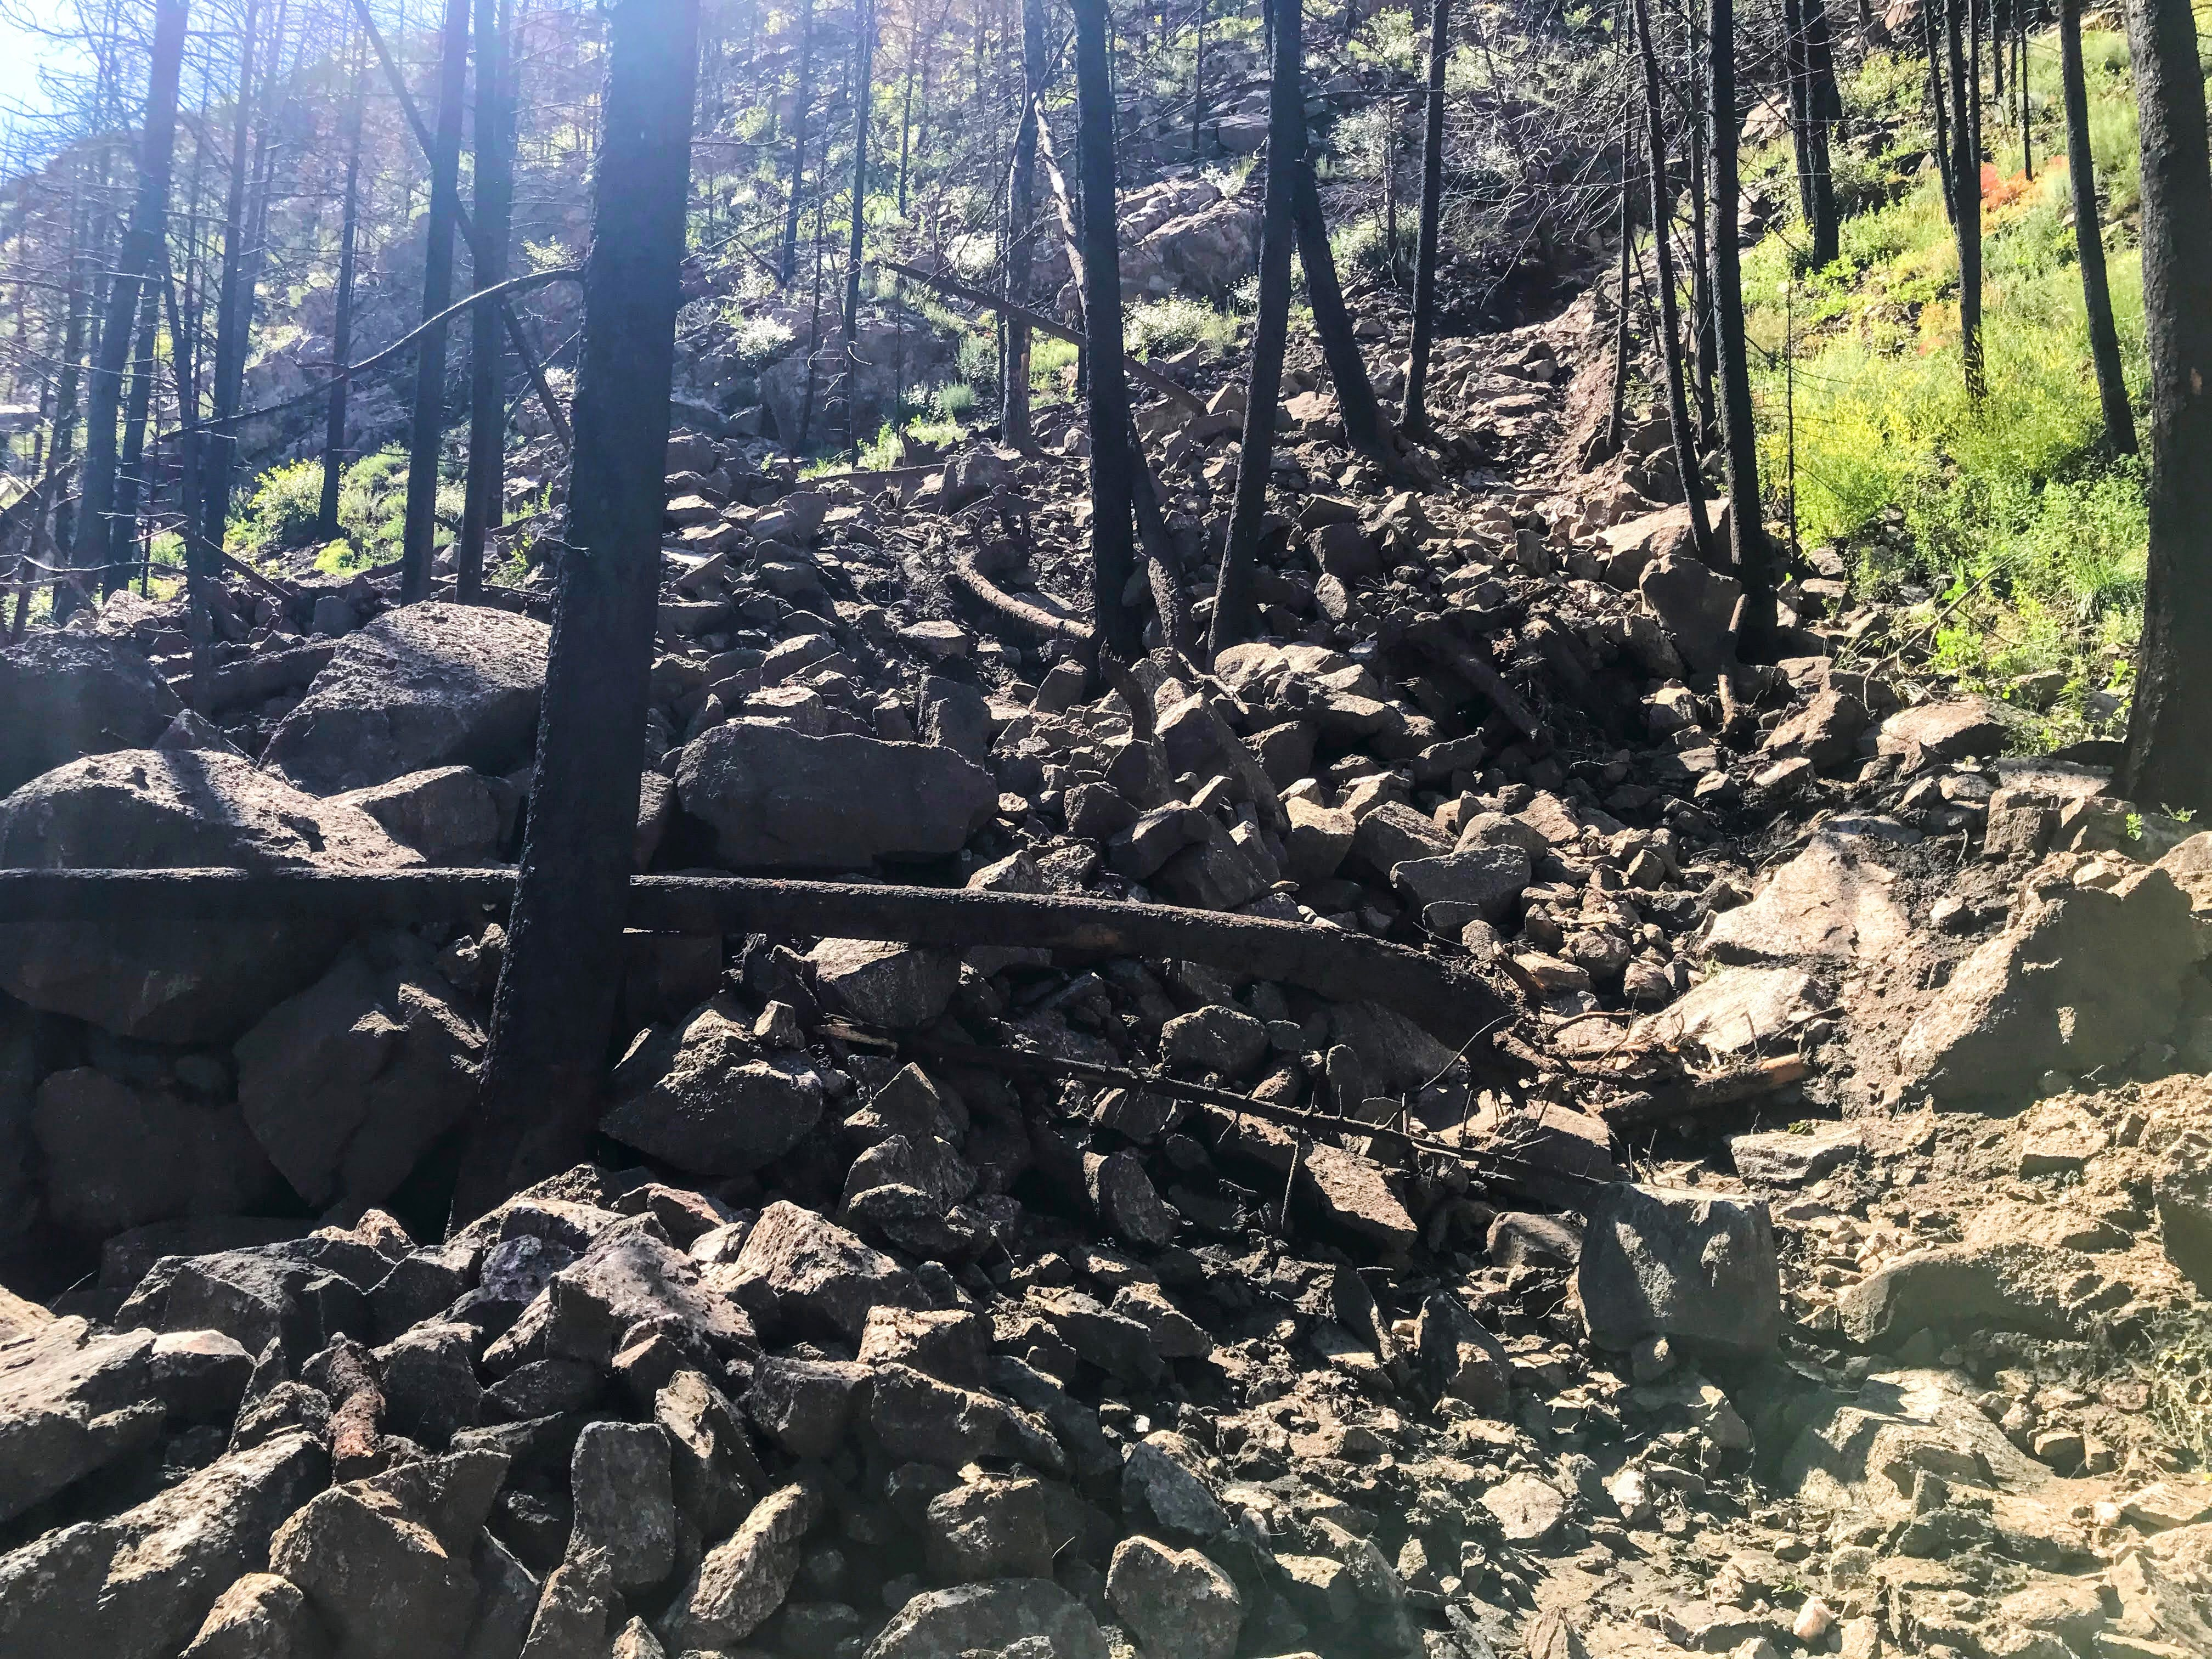
\includegraphics{../Images/debrisFlow} \caption[New debris flow deposits]{New debris flow deposits in a drainage near my family's house. Photo by author.}\label{fig:figureTitle2}
\end{figure}

On four different occasions during the summer of 2022, I was witness to extraordinary flooding events, as if the land had been cleaved open to let loose a deluge of water and sediment and boulders. Most of the channels in the Poudre Canyon --- a channel is a defined path created by the flow of water and sediment --- formed during the last Ice Age, about 18,000 years ago, according to a fluvial geomorphologist who designed post-fire flood mitigation structures in the Poudre. Although in my lifetime I had never observed any of the channels that come off the steep mountainside adjacent to our land to carry water in them, the existence of channels indicates the flow of water in geological time and the certainty of future flow. Whether channels flood with water and sediment or with debris, resulting in a debris flow, depends on how much debris has accumulated in the channel over hundreds or thousands of years through the process of erosion, aided by gravity, enacting its ``primary agency'' (\citeproc{ref-gordilloGravityPrimacyTerrain2020}{Gordillo 2020}) on the terrain. In the days following each flooding event in the summer of 2022, I hiked to every channel and sometimes to their origins up near the top of the ridgeline, to document what had tumbled down the mountain. I took hundreds of photos, organized these in photo albums, and labeled each one. Later, this documentation became useful to geologists at the United States Geological Survey (USGS) who study landslides and debris flows. They were able to use my photos to verify debris flows had occurred on a particular date and cross-reference these with data from the nearest rain gauge to develop a metric of debris flow susceptibility.

This was not the only data gathering I participated in on behalf of other researchers. These activities benefited my own engagement with the material world, my familiarity with different kinds of research which intersected with wildfire in some way, and my own curiosity. I collected water samples for research on the biogeochemistry of post-wildfire watersheds; documented how flooding impacted installed flood mitigation structures through photos and emails for the consulting company who had designed the installations; and reported flash floods to the National Weather Service (NWS) as a weather spotter. I also facilitated connections between people. I put researchers in touch with landowners and landowners in touch with flood mitigation specialists; I connected a person installing beaver mimicry structures --- intentionally placed wood mimicking beaver dams, which catch sediment and slow down the flow of water --- and facilitating beaver habitat recovery with a wildlife biologist who is tasked with removing ``problem beavers''. The thought was that the problem beavers could be relocated to areas where beavers would aid riparian recovery.

USGS geologists, along with a geologist from the Colorado Geological Survey, came in the summer of 2023 to visit my family's land and another site farther up the canyon, to see debris flow deposits in person. At the bottom of one of the channels, there was a large boulder perched on the edge of a steeper chute below it. From the house, the boulder looks poised to fall, and I remember watching it the summer before each time there was flow down the channel, waiting for it to spill down the channel. But it never did. ``That one will go in the next hundred years,'' one of the USGS geologists said glibly as we bushwhacked our way out of the aspen grove. Geology time, I thought. Along with mapping emergent plant species, mapping flood events became another aspect of my fieldwork in the summer of 2022, documentation which enabled my participation ``in the world's transformation of itself'' (\citeproc{ref-ingoldBeingAliveEssays2011}{Ingold 2011}).

I shared, with my neighbors and interview participants, a continued engagement in sensemaking in relation to the transformed landscape of the Poudre Canyon. Post-wildfire, senses of place are reformulated based on an ongoing, more tenuous relationship with the environment. Following transformative and sometimes destructive wildfires and flooding, sense of place is often disrupted (\citeproc{ref-schlosbergDisasterPlaceJustice2020}{Schlosberg, Della Bosca, and Craven 2020}). One person lost her cabin that had been in their family for four decades during a catastrophic and deadly debris flow, which rendered the area where their cabin used to be unrecognizable. Talking about the difficulty of reconciling her relationship to place before and after the debris flow, she said ``sometimes it's almost a strange feeling because I feel like I have two memories now. I still remember this place, from childhood, growing up, and even just a few years ago, and then having to reconcile that with, it doesn't exist. It no longer exists'' (November 2022).

\begin{figure}
\includegraphics{../Images/blackHollow} \caption[Black Hollow house remains]{The house of a Black Hollow homeowner, on the left, prior to the debris flow, and the remains of his house in the river after the debris flow. Photos provided by Clyde Romero, Jr.}\label{fig:figureTitle3}
\end{figure}

My focus was continuously drawn to the weather, along with others in the Poudre, particularly those who live close to tributaries with potential for flooding. My neighbors and I exchanged information sources for emergency alerts and sent texts to each other tracking rain gauges on an interactive map which the county made available in 2023. How we interact with and experience the weather, which manifests within specific environmental contexts (\citeproc{ref-endfieldClimateCulturalHeritage2015}{Endfield and Naylor 2015}), is part of the process of reconciliation with a landscape we are coming to know again. Weather is an agentive force (\citeproc{ref-dewitTranslatingClimateChange2018}{De Wit, Pascht, and Haug 2018}) in the context of the wildfire which burned through this canyon and in the ongoing flooding events different members of the community experience. Over the summers of 2022 and 2023, I became a compulsive observer of the western skies out the windows, wondering with trepidation what that day might bring. I am reminded, in my behavior, of the anthropologist Frida Hastrup's description of survivors in a tsunami-affected village in South India, who seemed ``suspended in a matrix made of the presence of disaster and the absence of certainty'' (\citeproc{ref-hastrupMaterializationsDisasterRecovering2010}{Hastrup 2010}). This hyperfocus on weather, in concert with muddying my boots exploring the terrain after a flooding event, helped me better understand experiences of risk and vulnerability in a dynamic, familiar-turned-unfamiliar landscape. My sensory engagement with this landscape undergoing rapid changes helped build a sense of intimacy with this new world, and the hazards associated with it, what I refer to as recalibration in Chapter 4.

\begin{figure}
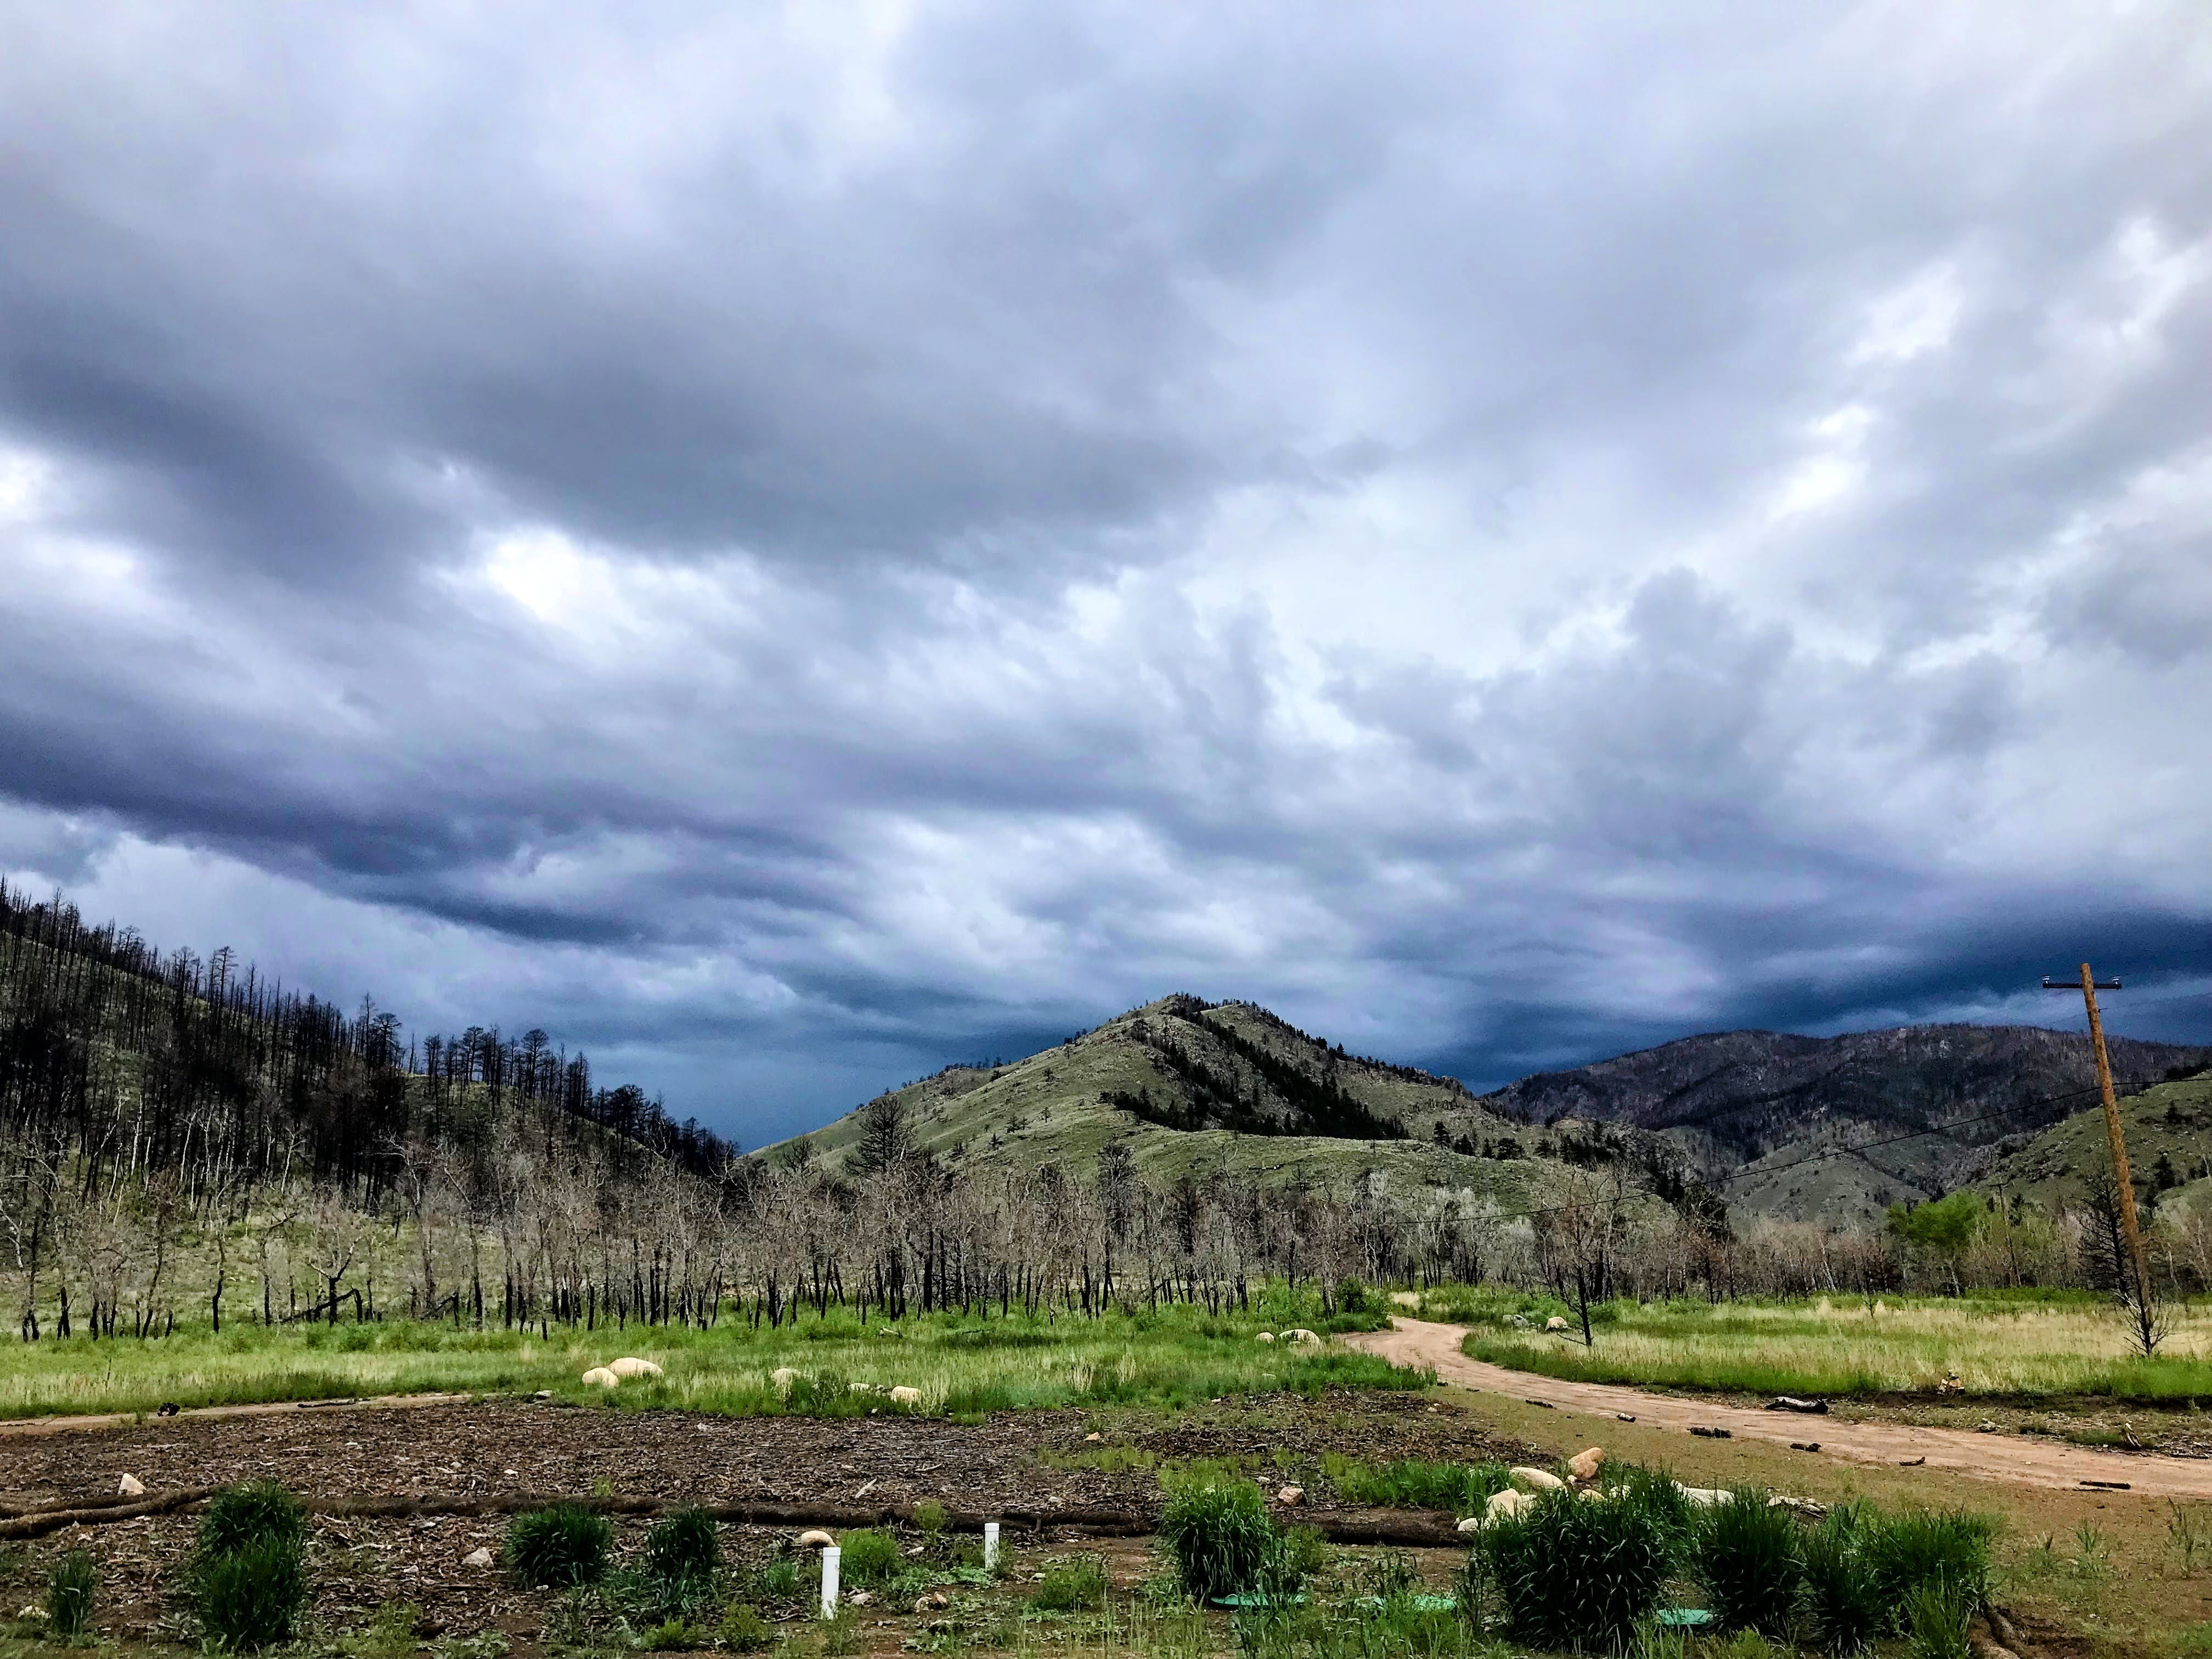
\includegraphics{../Images/clouds} \caption[Sky looking west]{The sky looking west from my family's house in June 2023. Photo by author.}\label{fig:figureTitle4}
\end{figure}

My approach to being in, on, and around the landscapes of the Poudre were informed by the way I affectively encountered the world, which is simultaneously experiential, classificatory, and emotional. Walking in areas of the CPF burn area with different subject matter experts, whether fire managers or fluvial geomorphologists, provided me with fresh perspectives on forest ecologies, on ecological functions of flooding, and contemporary forest management practices. My deeply situated and embodied landscape-based approach was also methodologically important for engaging with the materiality and temporality of wildfire and the cascading hazards affecting ecological processes and people's lives.

\subsubsection{Engaging With `Experts': Walking and Talking with Researchers, Scientists, and Fire Practitioners}\label{engaging-with-experts-walking-and-talking-with-researchers-scientists-and-fire-practitioners}

When deciding to live on my family's land for a year during my fieldwork, I had not anticipated that the land itself --- and the water running through it --- would be the basis for walking conversations about matters of interest to scientists and an enticement in and of itself for those studying aspects of post-wildfire recovery. In my introductory emails to fire and water managers and forest and fire ecologists and geologists, I described what had happened to my family's house and the trees on our land and the subsequent flooding on our creek. Along with the choices of meeting over Zoom or traveling myself to meet them in person, I also offered prospective interviewees the option to meet at my family's place. Of the fifty interviews I conducted, eleven were conducted at Pinehurst, and several other scientists I did not interview subsequently visited my family's land, to examine debris flow deposits or to observe the way the fire had behaved in different areas, resulting in the death or survival of certain trees. Thus my family's land, and the way in which fire and flood had interacted with it, became a part of my own methodology, intertwined with the way it was part of the methodology for others who initiated research there before or after our in situ meetings.

I met a fluvial geomorphologist and professor of geology at Colorado State University at my family's place one afternoon in June 2023, a day after a significant flooding event on Sheep Creek, whose headwaters originate on Forest Service land before it flows through our neighbor's land and then our land in its lower reaches before emptying into the Poudre River. Having never been to my family's land before, she was able to apprehend material flows and processes at a glance and convey different ways of interpreting the landscape to understand, on a geological time scale, what had occurred in the past and what was currently underway. At one point on our walk along the creek, in a wider part of the valley where there was a large depositional zone (meaning the width of the channel was largely cobble and finer sediment), she pointed out what she called the ``birth of a new channel.'' This new channel had diverted to the side once the water hit the wide depositional area. We could see water coursing through live vegetation without any sign of the formation of stream banks yet.

I walked my family's land with a number of scientists and practitioners, outlined in Table \ref{table:IntroTable1} below. I refer to these as walking conversations, which are semi-structured interviews designed to use place, movement, and landscape to prompt connections and meaning to the surrounding environment (\citeproc{ref-evansWalkingInterviewMethodology2011}{J. Evans and Jones 2011}; \citeproc{ref-evansGroundingKnowledgeWalking2009}{C. Evans et al. 2009}; \citeproc{ref-berroetaPlaceSubjectivityContinuum2021}{Berroeta, de Carvalho, and Castillo-Sepúlveda 2021}), in which ``the complex surface of the ground is inextricably caught up in the very process of thinking and knowing'' (\citeproc{ref-ingoldFootprintsWeatherworldWalking2010}{Ingold 2010}: S135). Of the thirteen people listed here, I interviewed eight. In some cases our walking conversations supplemented more formal, recorded conversations. In the cases where no formal interview occurred, these walking conversations constituted a particular kind of participant observation, with landscape as its basis. Subject matter experts engage in sensemaking, too, both through the lens of their knowledge production and their own personal experiences with fire and forests and flood. These walks were a window into their work and their worldviews. All of these interactions opened up a new way for me to see and experience my family's land and post-wildfire landscapes in general, a kind of recalibration of my previous knowledge holdings.

\captionsetup{width=6.5in}

\begin{table}[!h]
\centering\centering
\caption{\label{tab:IntroTable1}Walking conversations.}
\centering
\begin{tabu} to \linewidth {>{\raggedright}X>{\raggedright}X>{\raggedright}X}
\toprule
Role & Organization & Jurisdiction\\
\midrule
Forest ecologist & Colorado State University & University\\
Fire ecologist & Colorado Forest Restoration Institute & University\\
Fuels technician & Bureau of Land Management & Federal\\
Research biogeochemist & Rocky Mountain Research Station & Federal\\
Fire behavior analyst & Colorado State Forest Service & State\\
\addlinespace
Fluvial geomorphologist (2) & Colorado State University & University\\
Fluvial geomorphologist & Consultant & Private\\
Water manager & Front Range City & Municipal\\
Research geologist (2) & U.S. Geological Survey & Federal\\
Geologist & Colorado Geological Survey & State\\
\addlinespace
Fire manager & U.S. Forest Service & Federal\\
\bottomrule
\end{tabu}
\end{table}

Not only did researchers and scientists walk my family's land with me, I also joined some of them in their fieldwork and in some cases contributed to data collection. One example of the latter case, which is ongoing, is to collect monthly water samples from the creek which runs through my family's land which is then analyzed by biogeochemists at the USFS Rocky Mountain Research Station (RMRS) out of Fort Collins. Volunteer coordination is managed through a nonprofit called the Coalition for the Poudre River Watershed (CPRW). This research helps water supply managers in Fort Collins and Greeley on the Front Range prepare for future wildfire and water quality mitigation plans and also helps evaluate post-wildfire watershed treatment strategies.

\begin{figure}
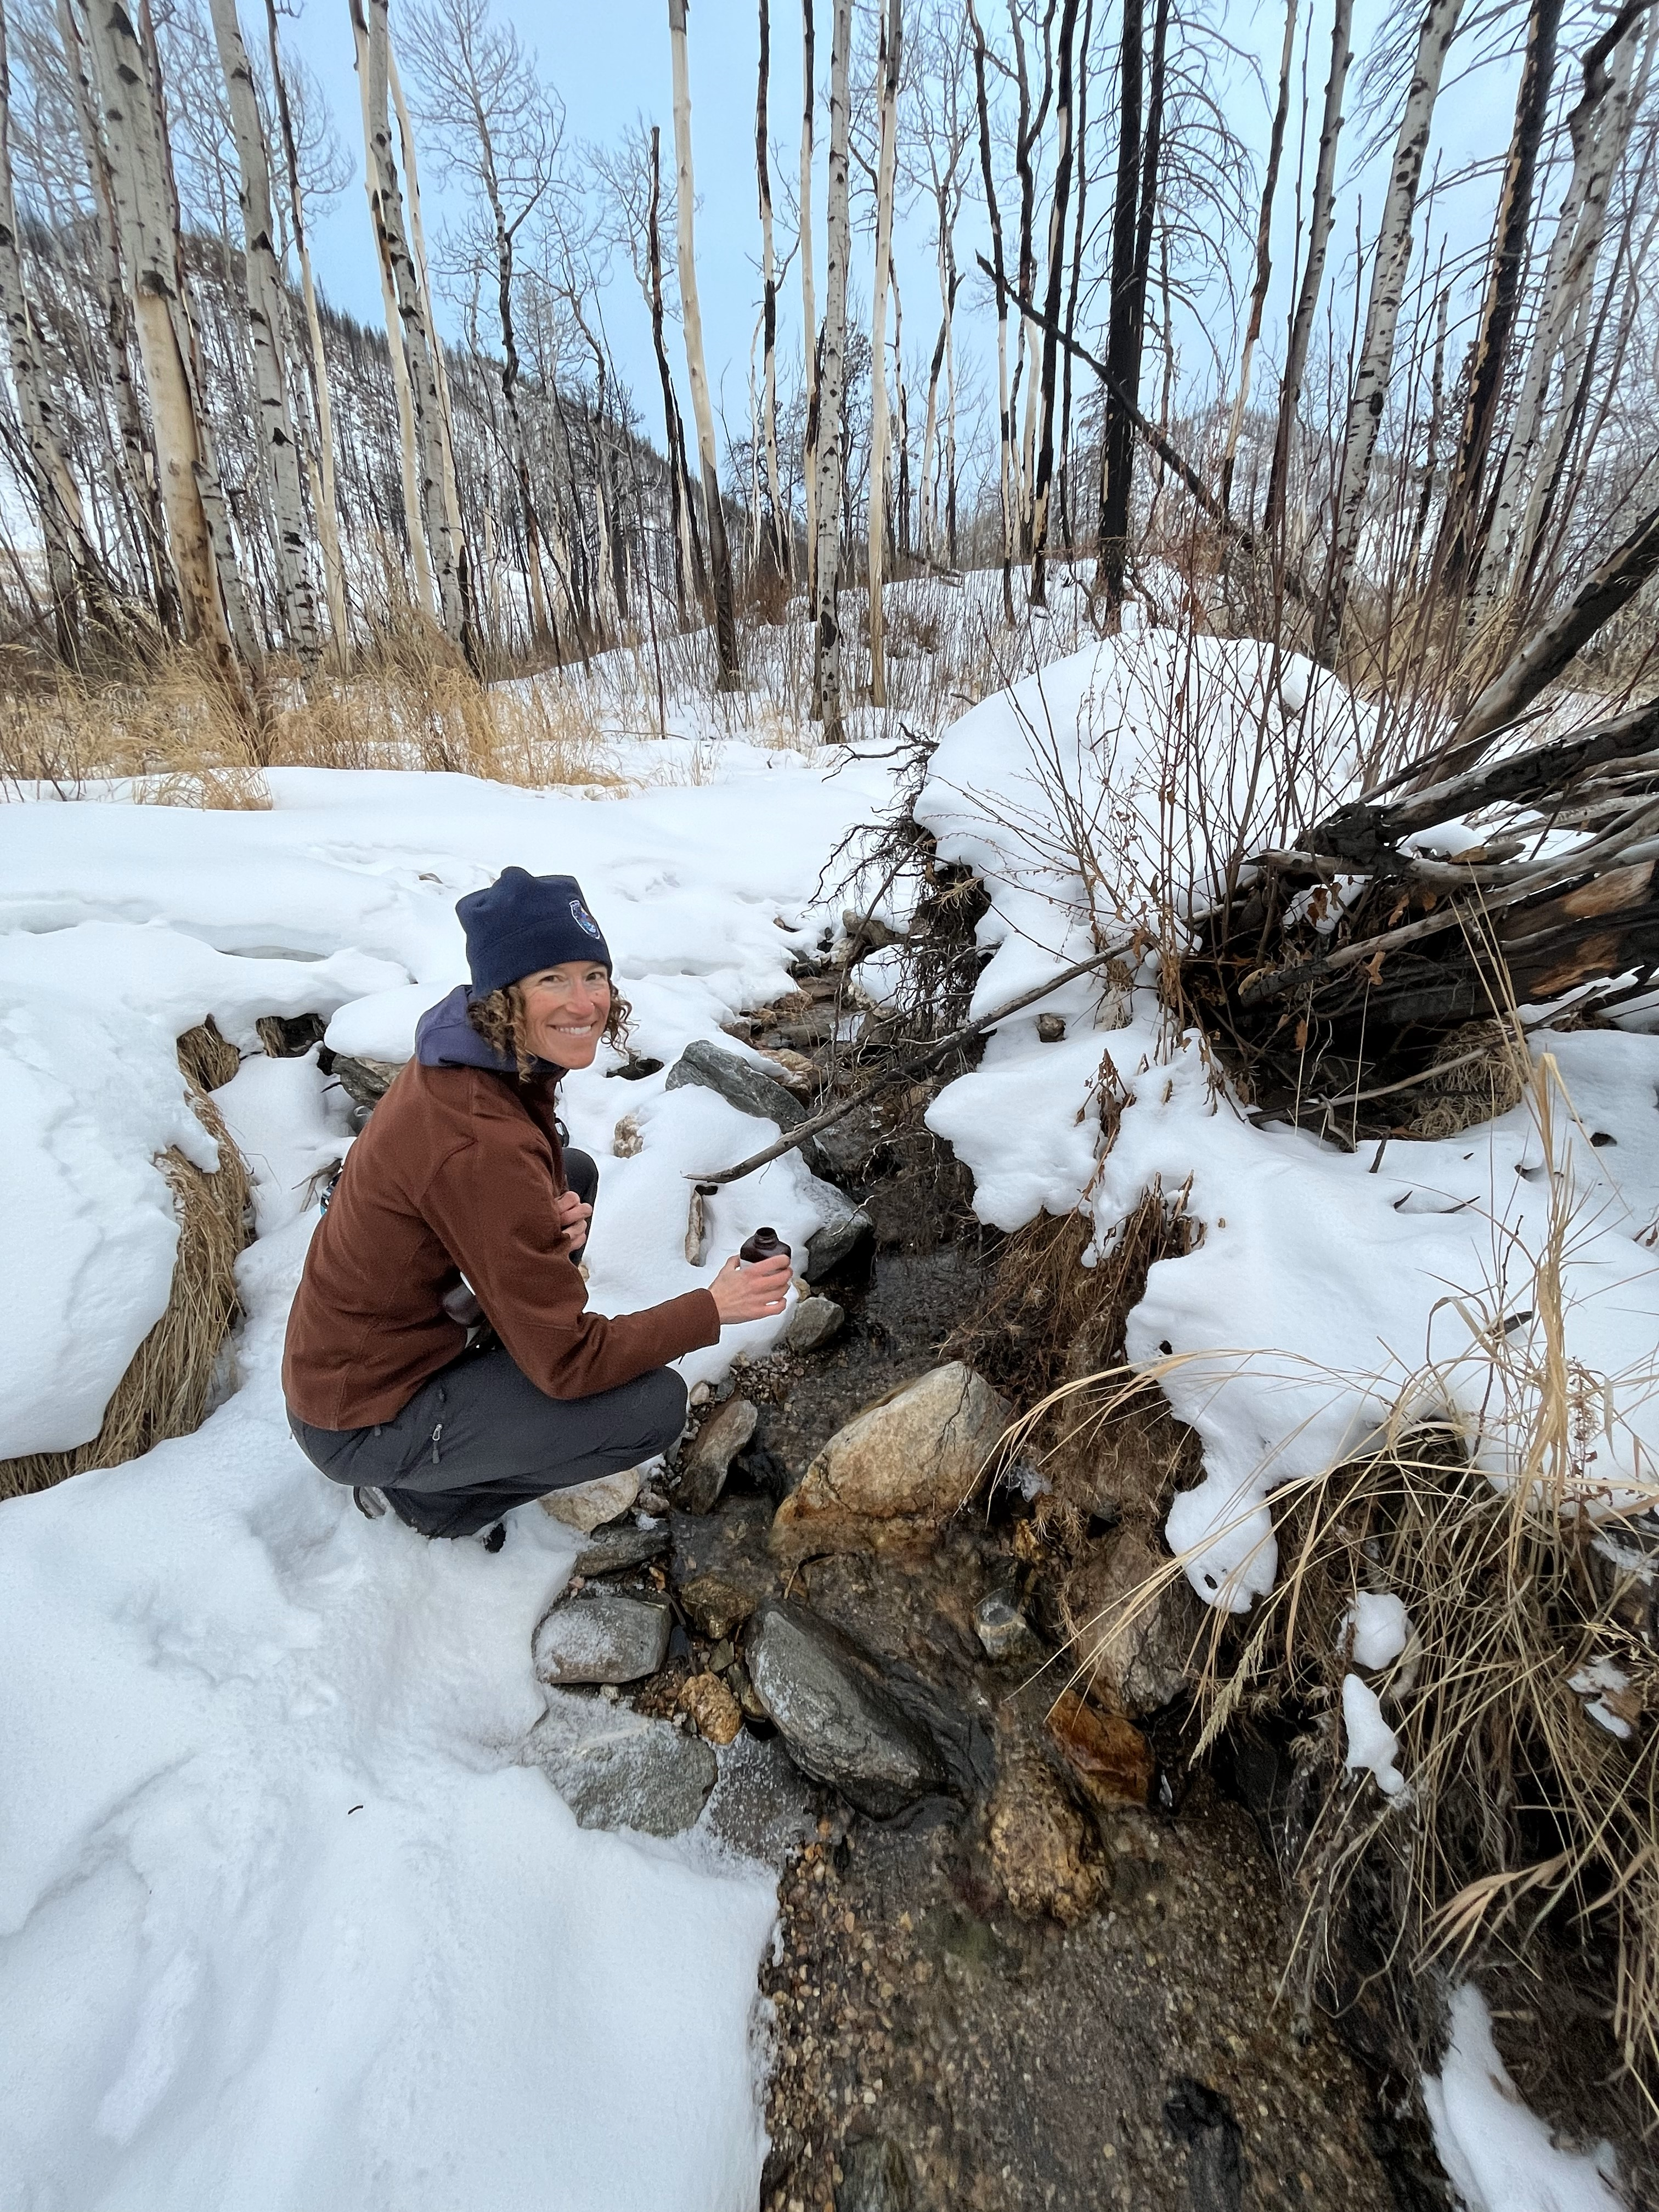
\includegraphics{../Images/waterSample} \caption[Sheep Creek water sample]{Taking a water sample from Sheep Creek for the RMRS in January 2023. Photo by Evan Stafford.}\label{fig:figureTitle5}
\end{figure}

On multiple other occasions, I accompanied field crews to collect data for different scientific research endeavors. These trips were opportunities for me as an ethnographer to engage in ``embodied learning'' (\citeproc{ref-maslenNarrativePracticeStorytelling2022}{Maslen 2022}), what is referred to as the go-along method (\citeproc{ref-carpianoComeTakeWalk2009}{Carpiano 2009}). This method ``engages the environment'' by ``placing researchers in the mobile habitats of their informants, thus facilitating access to their experiences and practices as they unfold in real time and space'' (\citeproc{ref-kusenbachStreetPhenomenologyGoEthnographic2003}{Kusenbach 2003, 478}). My trips into the field with various researchers helped me understand how subject matter experts come to see and know their subjects as a result of epistemological knowledge along with tactile engagement with the environment they study (\citeproc{ref-oreillySensingIceField2016}{O'Reilly 2016}). How researchers moved through the landscape depended upon their field of knowledge, the data they collected, and what they were conditioned to notice through their own disciplinary training combined with iterative sensory engagement with their subject matter over time (\citeproc{ref-oreillySensingIceField2016}{O'Reilly 2016}). In Table \ref{table:IntroTable2}, I list the role of the lead researcher and how many crew members in parentheses, followed by the organization they work for, and their research focus on the day I accompanied them.

\captionsetup{width=6.5in}

\begin{table}[!h]
\centering\centering
\caption{\label{tab:IntroTable2}Go-alongs.}
\centering
\begin{tabu} to \linewidth {>{\raggedright}X>{\raggedright}X>{\raggedright}X}
\toprule
Role & Organization & Research Focus\\
\midrule
Fluvial geomorphologist (2) & Colorado State University & Post-fire watershed survey\\
Fluvial geomorphologist & Colorado State University & Flow channelization\\
Research Biogeochemist (10) & Rocky Mountain Research Station & Biogeochemical longitudinal survey\\
Fluvial geomorphologist & Consultant & Flood mitigation tour\\
Research geologist (3) & U.S. Geological Survey and Colorado Geological Survey & Validation of debris flows\\
\addlinespace
Research geologist (3) & U.S. Geological Survey & Debris flow deposit volume measurements\\
\bottomrule
\end{tabu}
\end{table}

\begin{figure}
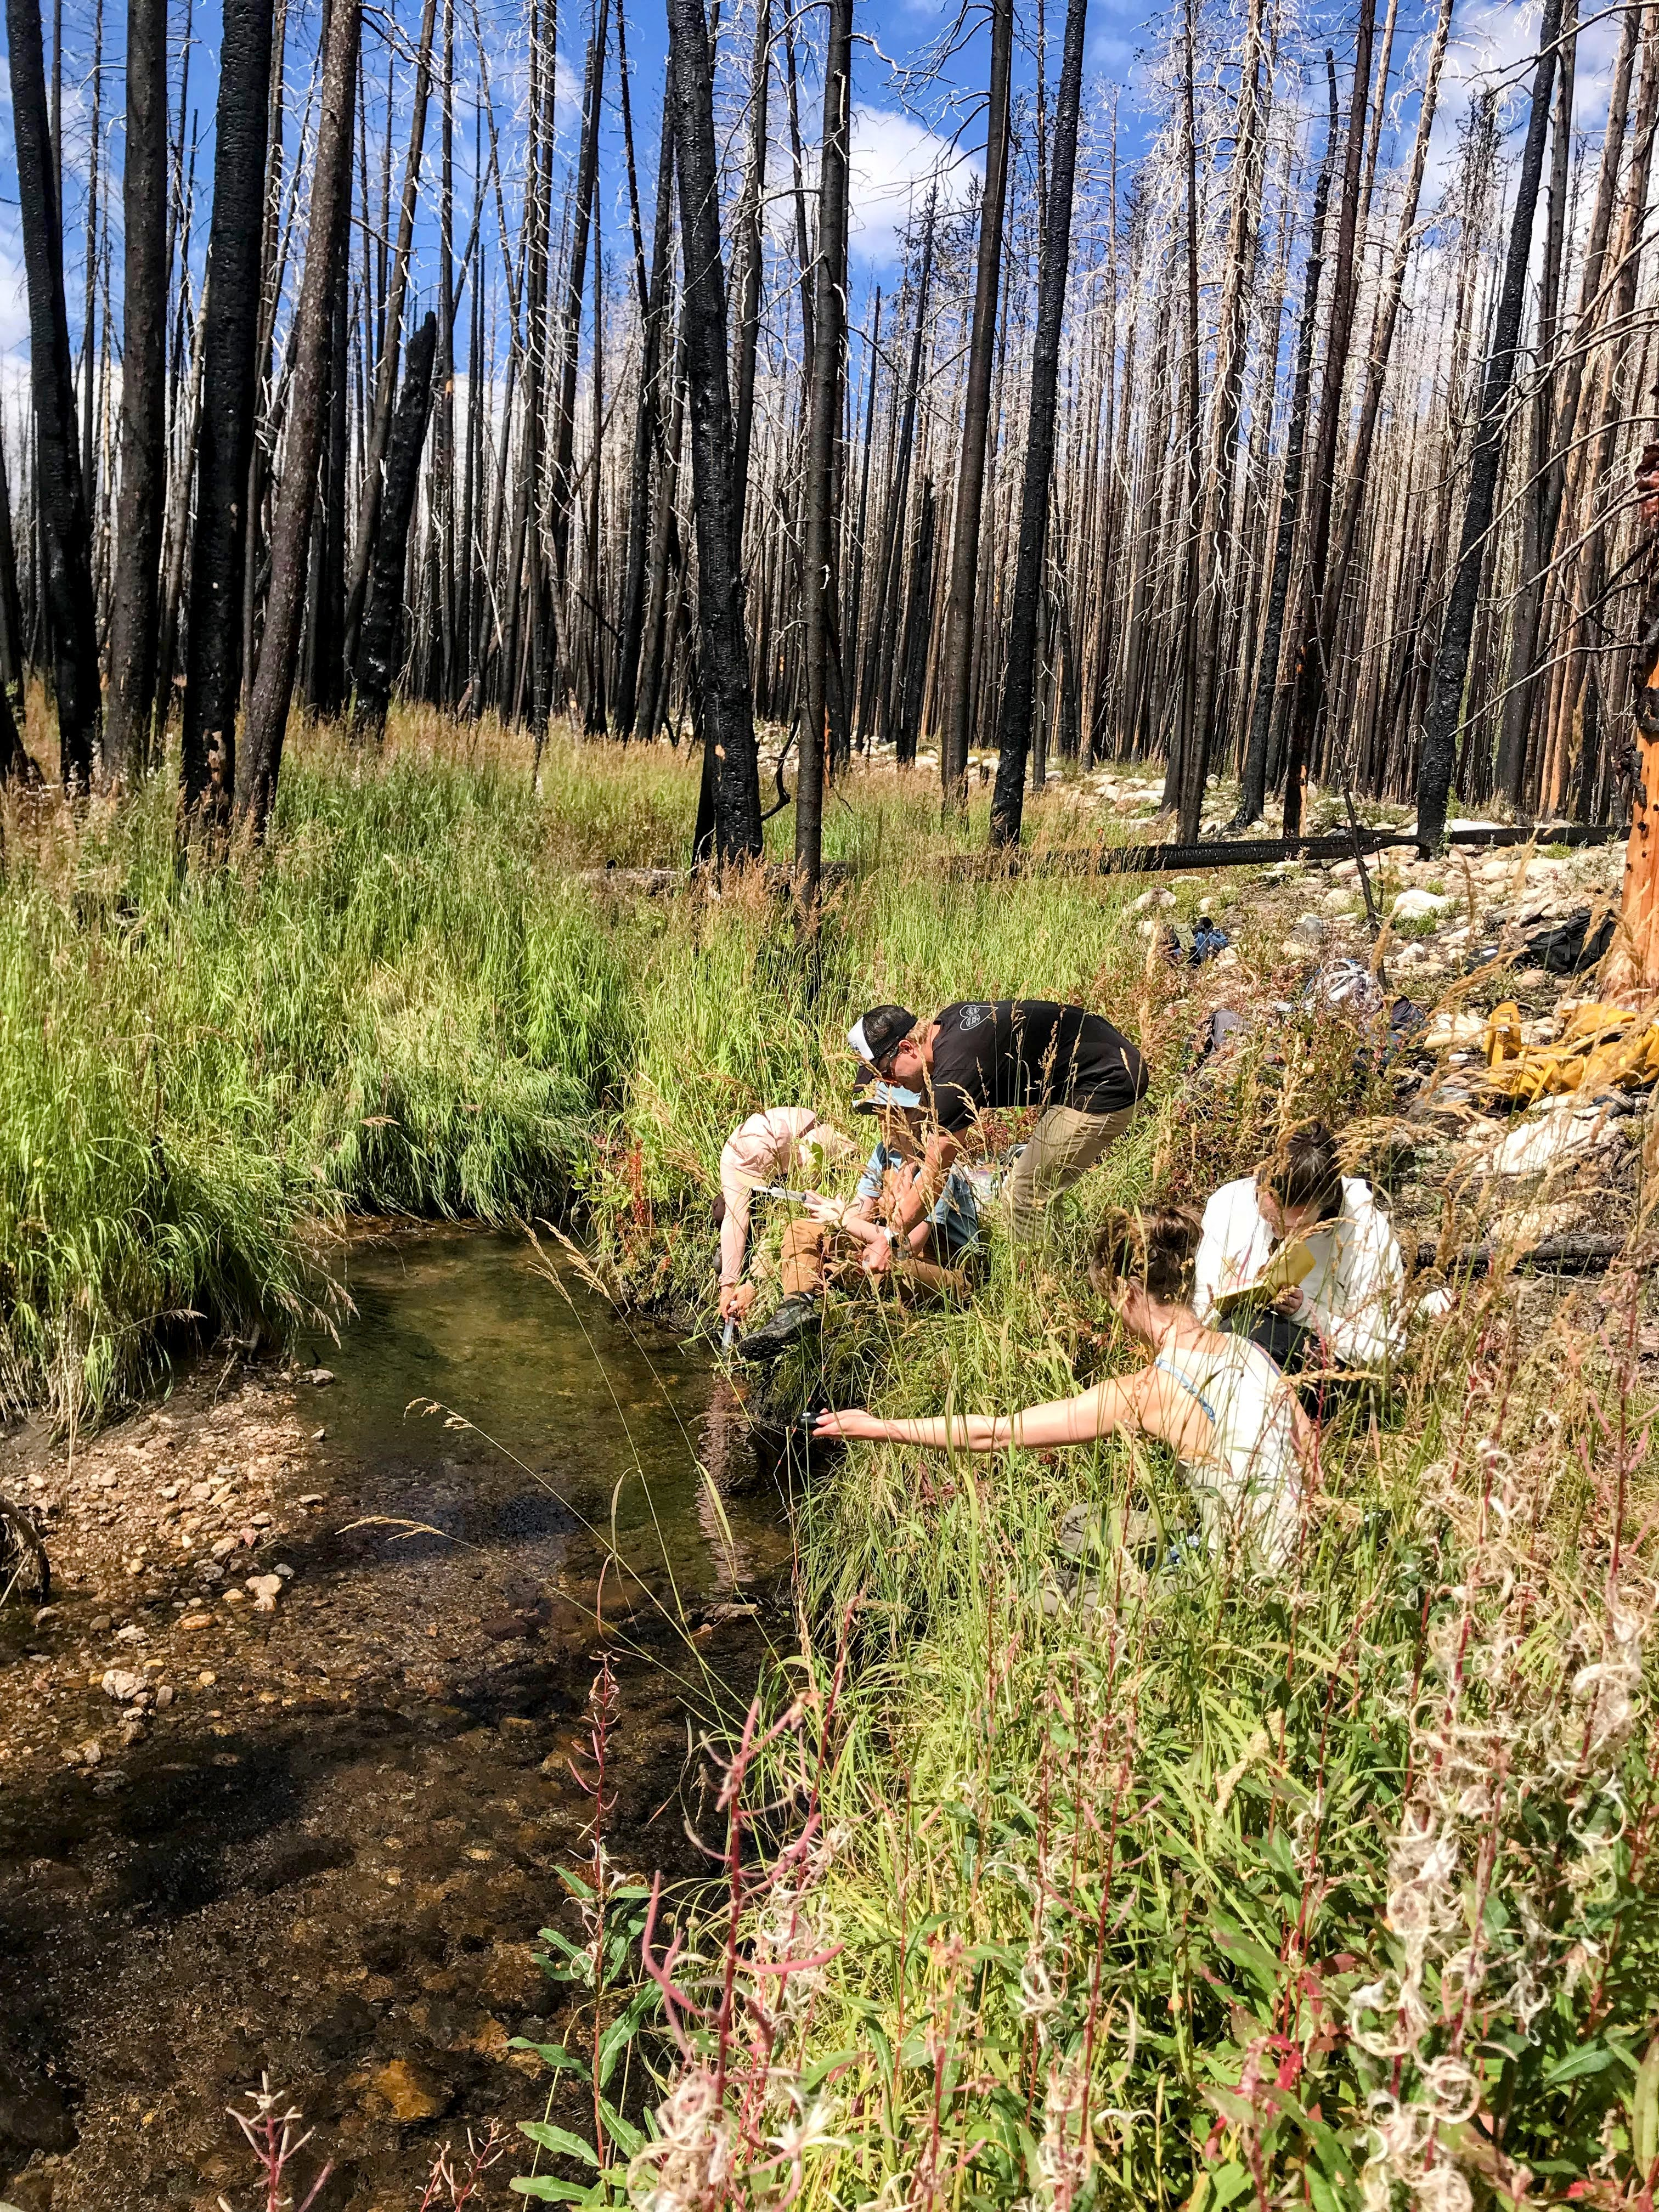
\includegraphics{../Images/LBC} \caption[Little Beaver Creek survey]{Field crew with RMRS taking various measurements at a presumed biogeochemial hotspot along Little Beaver Creek. Photo by author.}\label{fig:figureTitle6}
\end{figure}

On one of the days I accompanied scientists in their field research, I joined two fluvial geomorphologists --- someone who studies the movement of rivers over time and how they shape landforms --- who were conducting a watershed survey to determine what geomorphic factors contribute to watershed resiliency to wildfire. They collected empirical data about the tributary we walked from top to bottom, counting the number of channel jams --- in-stream piles of wood --- and floodplain jams --- piles of wood deposited outside of the channel on the floodplain --- as measured within a defined reach. A reach is a segment of stream defined by its characteristics. I learned that one of the ways that streams are resilient is in their complexity, conceptualized as the numbers of beads along a string (\citeproc{ref-wohlRiverBeadsConceptual2018}{Wohl, Lininger, and Scott 2018}). A stream that is mostly string has less complexity than a stream with lots of beads, which may be areas of sinuosity, beaver dams, multiple channels, and other mechanisms that facilitate vertical and horizontal connectivity in a stream, such as log jams and piles of wood deposited on the floodplains. Floods or debris flows can also facilitate greater complexity and introduce beads into the system, at the same time that they can create longer strings by blowing out areas of greater complexity.

\begin{figure}
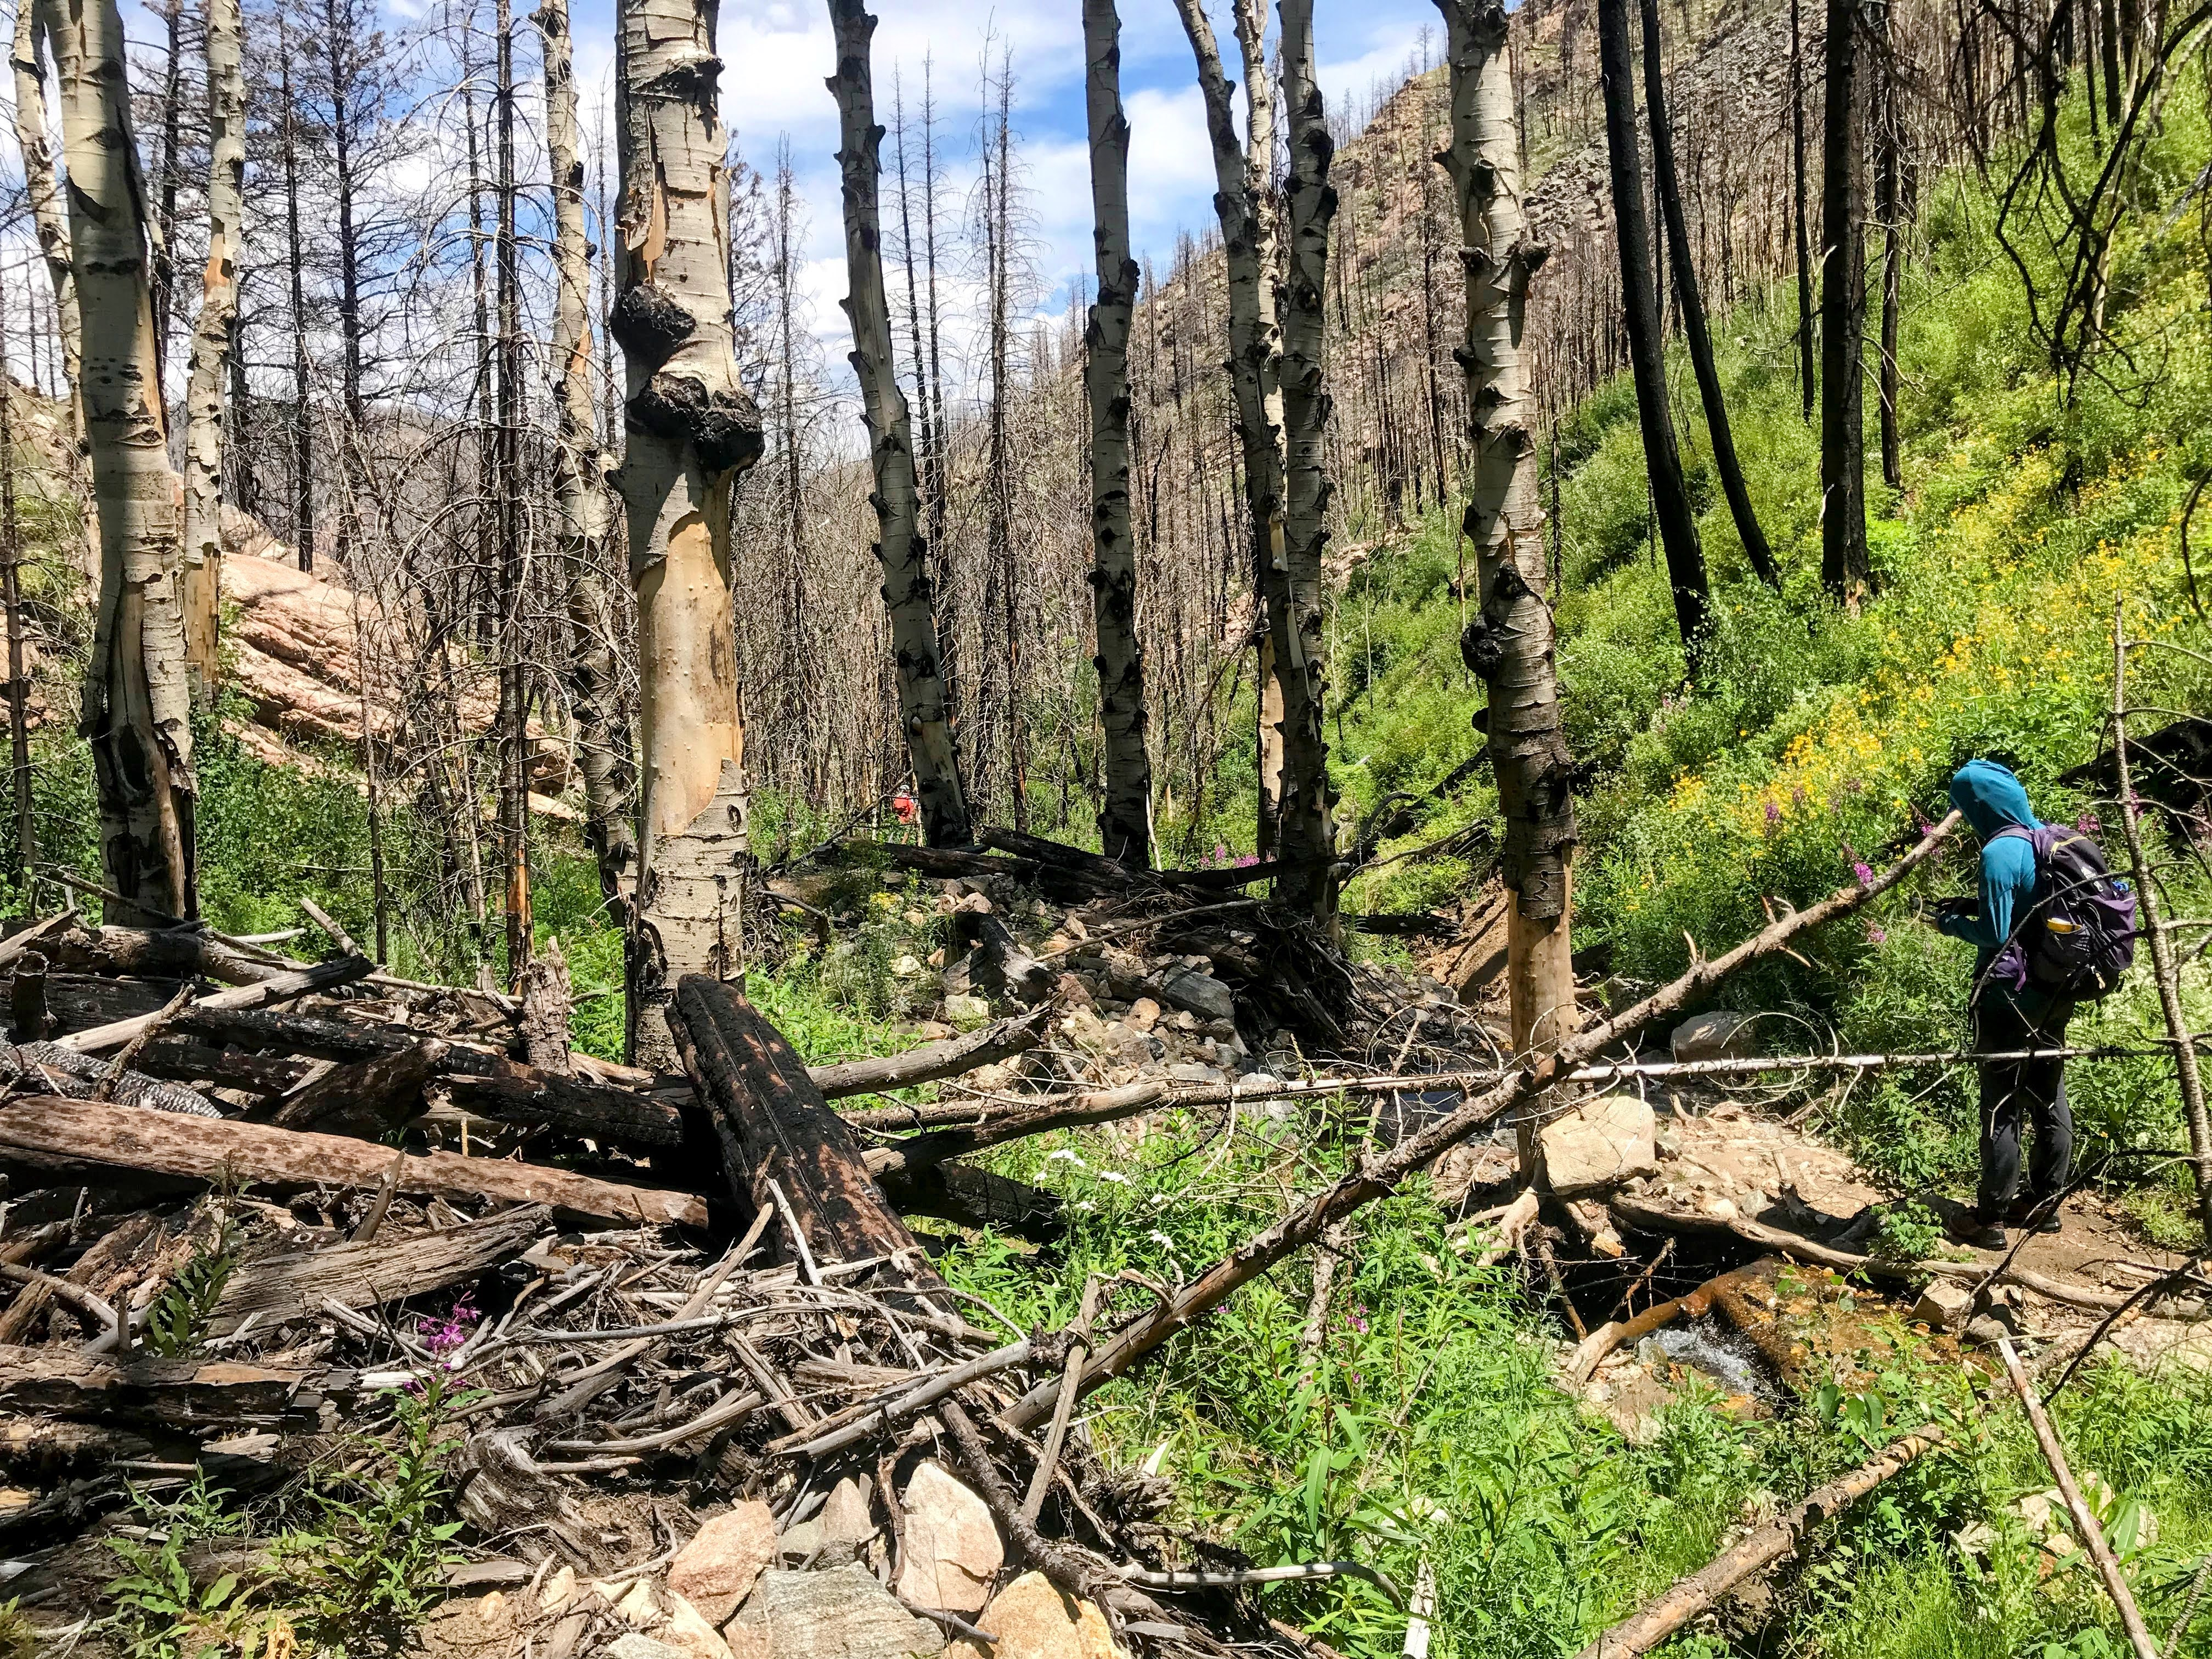
\includegraphics{../Images/sheepGulch} \caption[Sheep Creek survey]{Counting floodplain and channel jams on a watershed survey of Sheep Gulch. Photo by author.}\label{fig:figureTitle7}
\end{figure}

Part of my process of knowing wildfire and its ecological linkages is facilitated by accompanying people like the fluvial geomorphologists, moving across a landscape or through a waterway paying attention to things I previously did not know how to ascertain. ``To physically move through land, by these various means, is also to travel through time and connect with the past. In other words, landscape binds up the past and present, and variously structures (pre-)history and holds knowledge'' (\citeproc{ref-evansGroundingKnowledgeWalking2009}{C. Evans et al. 2009}: 194). Understanding the ecologically beneficial aspects of wildfire and flooding --- which include benefits for human lives --- and contextualizing these processes within their own timescales are two different processes of learning to see. They also happen successively. The wildfire sweeps across the land, transforming it in its wake. Long before one becomes familiar with this landscape altered by fire, it is transfigured yet again by flooding, in entirely new and devastating ways, at least for human lives and the built environment. As human beings with memories and experiences situated in a particular kind of landscape unscathed by a wildfire the scale of Cameron Peak Fire, it takes time to become situated again. For some, this adjustment never happens. One woman who used to live in the Upper Poudre as an adult and whose family sold their cabin in 2023, in the family since the 1960s, no longer considered the canyon beautiful after the burn, one of the ways she reconciled selling their family home.

Walking over debris fields and in stream channels and over logs with researchers and scientists rendered the landscapes of the Poudre Canyon and surrounding areas as a `lived phenomenon' (\citeproc{ref-cresswellLandscapeObliterationPractice2003}{Cresswell 2003}: 281), as unfinished, embodied, and practiced, where my previous life experiences had rendered it fixed both in imagination and experience. This is perhaps because the way in which we ``come into relations with other things conditions what we know about them'' (\citeproc{ref-root-bernsteinThingsThatAre2019}{Root-Bernstein 2019}). My explorations of my family's land and my participation in different kinds of fieldwork in other watersheds helped me conciliate my visceral experiences of fire and flood as destructive forces with an appreciation for their ecological and geomorphic functions in their own right, in a manner that both transcends the human experience and intersects with it in complicated ways, simultaneously beneficial and disastrous.

Undeniably, wildfires and flooding can have devastating consequences for people's lives at the same time that they can be not only ecologically beneficial over time but ecologically necessary, in ways that also benefit human beings. Part of my methodological approach, rooted in walking and talking with subject matter experts, helped me locate my life history and my family's history within the context of the multiple materialities, temporalities, and agencies of ecologies, terrain, weather, climate, and human actors. It enabled me to see the landscape beyond the context of my own life experiences and observations before the fire and to understand it within the context of its own ecological and geological histories and patterns and through the lens of other knowledge systems and worldviews.

\subsubsection{Community Involvement}\label{community-involvement}

I intended for my participation in the community to be diverse and to know people in as many ways as possible. The nature of doing my fieldwork in a sparsely populated, rural area with few services necessarily limited the ways in which I could be in community. The entire Poudre Canyon has a full-time population of 750 residents stretched over forty miles, with 1,500 residents in the summer (\citeproc{ref-Us2024}{{``About {Us}''} 2024}). The two main centers of population, one in the lower canyon and one in the upper, are nearly forty minutes apart by car. My fieldwork was mainly focused in the upper Poudre because only this part of the canyon was impacted by the Cameron Peak Fire. The lower Poudre was heavily affected by the High Park Fire in 2012. I interviewed several people who live or used to live in the lower Poudre and came to know others through another form of involvement, which was volunteering for the PCFPD. I discuss this further in the next section.

I participated in most scheduled gatherings in the upper Poudre throughout the course of my fieldwork. These include two monthly meetings, one for the Fire Board, and one for a member-based community organization that has been around for decades. This organization typically holds an annual fair. There are weekly non-denominational church services from April to September at a vaulted chapel built with community labor on donated land in the 1950s, from whose pews one can see the river out the windows. Game night is also held weekly. There is one restaurant in the upper Poudre, where a weekly community breakfast is held, which I attended regularly for a period of time. Women gather monthly for bookclub, and weekly for Ladies Tea, previously known as Peacemakers and primarily a craft group. Men meet for Men's Coffee on a weekly basis. Aside from regularly scheduled social activities, there were intermittent gatherings to cut firewood for those in need, to help a neighbor whose family shrine was heavily damaged in the CPF, a pie social, and a community work day to remove fuels (i.e.~dead or living vegetation) from around a cluster of community buildings, among other things. All of these activities enabled me to speak with people about their perspectives and experiences related to the fire and post-wildfire flooding, especially those people whom I did not interview.

\subsubsection{Demographics}\label{demographics}

It is difficult to collect demographic data systematically in the Poudre Canyon because though there are several areas with clusters of houses, many other homes and the people who own them are stretched longitudinally over many miles, obscured by trees, located over private bridges, or otherwise inaccessible to a roaming anthropologist. My familiarity with those in the upper Poudre community is limited by my prior acquaintance with families whose histories have intertwined generationally with my own, by who chooses to attend structured social events, by my involvement with the PCFPD, and by the multiple places I resided over more than two years, where I met people who live in different areas of the upper Poudre. Aside from the community center and chapel, there are few places for people to gather socially. There are just two restaurants the entire forty-mile length of the canyon, spaced about a half hour's drive apart. There is no longer a school. The one-room schoolhouse which my sister and cousins attended was closed by the school district in 1994. When my mother was a child, there were multiple other families with children, and this was true, albeit to a lesser extent, when I was a child, too. Today, the upper Poudre is primarily a retirement community on fixed incomes. It is almost entirely white and English speaking, with a handful of exceptions. To my knowledge, there are a handful of people who live here and continue to work full-time, remotely, as commuters, and with local jobs. Local work includes construction, restaurant work, garbage service, custom ammunition supply, and resort ownership. Retirees' former jobs include plumber, nurse, administrative assistant, engineer, and firefighter, among others. There are five resorts and one commercial campground in the upper Poudre, one which includes the only restaurant. This resort also has an RV park, and some of the RV campers work part-time at the store or clean cabins in exchange for a place to stay. Four of these resorts have storefronts with fishing gear, snacks, and essentials such as milk. All of them have cabins to rent, with two resorts offering a rustic cabin experience with some of the cabins dating back to the late 1800s and early 1900s. When the commercial campground was put in, sometime in my late teens, they installed a security light which could be seen from my family's house and our neighbor's house across the valley, the first source of real light pollution in this part of the canyon. In response, my neighbor began live trapping packrats --- a rodent which finds its way into homes and sheds and builds large, odorous prickly nests --- and releasing them near the campground in a hilarious but futile form of passive protest.

There are a disproportionate number of second homes to primary homes, although I do not know exactly how many. Unlike in many mountainous communities in Colorado, the majority of second home owners here are not affluent, just like the majority of residents are not high income. It is neither an impoverished --- there are certainly a few individuals who are very poor --- nor a rich community. There are few new homes being built because of the lack of new real estate, and one won't find in the upper Poudre multi-million dollar homes typical of many mountain communities in Colorado today (\citeproc{ref-blevinsSourceColoradosHigh2022}{Blevins 2022}; \citeproc{ref-MountainMigrationReport2021}{{``The {Mountain Migration Report}''} 2021}). Along with significant settlement in the late 1800s, the next largest influx of homes followed the sale of a cattle-turned-dude ranch in the 1960s, which was subsequently subdivided. The majority of homes originate from these two eras, with a smattering of others being built since then. Moreover, it has always been a community consisting of a good percentage of second homes, dating back again to the late 1800s. During the initial years of colonial settlement in the mid- to late 1800s, this community was composed of ranchers, fur trappers, miners, tie-cutters, construction workers, business owners, and people who retreated to the mountains from Denver or Fort Collins or Kansas or Nebraska for respite. During my mother's youth, there were several other families with children her age who spent their summers in the Poudre like she and her sisters did, other children whose parents were ministers or, like hers, teachers. This pattern of retreating to the mountains was typical of other mountain canyons near the Front Range of Colorado, where most of the state's population resides in cities. Unlike these other canyons, the Poudre has not grown exponentially and has remained a mountain residence and retreat largely for the middle class. This may be changing. Housing prices have, in accordance with the rise of costs around the state and an exponential hike in property taxes in Larimer County, begun to increase dramatically in the last few years. Recently a real estate investment firm purchased a large tract of land from a longtime family in the upper Poudre, and I learned from a construction worker there that they have purchased several other properties in the Poudre as well. It is difficult to foresee what their plan might be.

Although I do not know the histories of other mountain canyons in Colorado, I believe something unique to the upper Poudre is the longevity of connection to this place over generations. There are at least nine families and their descendants who have been in the Poudre since the late 1800s and continue to reside here, have generational family homes, or operate a resort. There are numerous other families who have had a presence here since the 1940s, 50s, and 60s and numerous others who have been visiting here routinely since their childhoods and chose to retire here, building a home or purchasing one. Still others have never lived here but have continued to return over the course of their lives to stay at one of the resorts and fish or hike or gather with family in the mountains, something I did not realize before I began living here full-time over two years ago. I recently learned of someone who has reserved an RV campsite at one of the resorts for thirty years.

New commercial development is severely limited by the county, which contributes to an overall sense among residents that the county, and the USFS, would prefer people do not live here. This is reinforced by decisions made by these different government actors with no visible presence here which greatly impact the lives of people in the Poudre but over which they have no input or control. As a rural, unincorporated area, the Poudre is administered by Larimer County with the oversight of three elected county commissioners. Most in person interaction with Larimer County is through the Sheriff's Department and Emergency Services, which is housed in the former. There is one visitor center belonging to the USFS, the largest landowner in the Poudre, which is staffed entirely by volunteers, both local and from elsewhere. A USFS archeologist is making a concerted effort to restore the cabins at the former lodge turned visitor center. Beyond this, there are few opportunities for residents in the Poudre to interact with anyone from the USFS, let alone anyone who is making decisions impacting their lives.

At the county level, one of the starkest examples contributing to the idea that the county does not want people to live here is the aforementioned removal of a private bridge and the lack of assistance in building a new one. Another example in relation to the USFS involves the property where the debris flow which damaged the bridge below occurred. The debris flow from the Black Hollow tributary was so massive that it changed the course of the river when it deposited trees and boulders into the river's path. A consulting company working with a coalition funded through the Emergency Watershed Protection (EWP) program of the Natural Resource Conservation Service (NRCS) to install flood mitigation structures was prohibited by the USFS from continuing its work. This was because the work would affect the river, sections of which were designated as Wild \& Scenic in 1986 (\citeproc{ref-CachePoudreWild1990}{{``Cache {La Poudre Wild} and {Scenic River Final Management Plan}''} 1990}). The USFS found that the consulting company had inadvertently not followed rules for using federal funds in relation to work that would affect a Wild \& Scenic-designated river and halted all work. The landowners at Black Hollow, six of whom lost their homes in the debris flow, now have a pile of boulders two stories high and a huge stack of logs with which to contend, material which sits on private property where there used to be homes, adding to the difficulty of rebuilding or selling their lots.

\subsubsection{Gender Dynamics}\label{gender-dynamics}

The social structure of the upper Poudre can be old fashioned, specifically in how certain key activities are gendered. This may be due in part to the fact that most people who live in the Upper Poudre are post-retirement age, although there are perhaps a dozen people in their 40s and 50s. Although I did not survey political or religious persuasion, based on informal conversations throughout more than two years of living here, the upper Poudre leans politically conservative and religious. These may also be factors in gendered social activities. In addition to Men's Coffee and Ladies Tea, the weekly breakfast is also gender segregated, with all the men at one table and all the women at another. This did not preclude me from interacting with and interviewing men as well as women, particularly through my involvement with the PCFPD. However, structured, regularly scheduled social activities were often organized to separate men and women, and I was excluded from certain spaces as a woman. Traditional gender roles surfaced in some areas, even while they were bucked in others. Dinner is made by different women for the fire district's monthly training, for example, never by men. Both men and women volunteer for the district and attend the trainings and drive the emergency vehicles. Just one person, a woman, drives the water tender, a fire truck with a large capacity tank on it. Although this dissertation does not specifically include gender analysis, it was a notable part of the social relations of the upper Poudre and shaped how and when I crossed paths with different groups of people. Gender ``as a culturally and politically constructed phenomenon'' (\citeproc{ref-ortnerFemaleMaleNature1996}{Ortner 1996}: 180) is often taken for granted by anthropologists working elsewhere, particularly in the Global South (\citeproc{ref-adhikariGenderedConsequencesSocial2022}{Adhikari and Sharma 2022}), but it is also the case right here at home.

In the Fall of 2022, I began regularly attending Ladies Tea. Most of the women brought craft projects to work on, and sometimes there were collective quilt projects, often led by the talented Jennifer. While she was evacuated from her home during the Cameron Peak Fire, living in a hotel room in Fort Collins, she created a quilt of a wildfire scene, a sky of billowy clouds of smoke over forested mountains on fire with the river coursing below.

\begin{figure}
\includegraphics{../Images/quilt} \caption[Cameron Peak Fire quilt]{The Cameron Peak Fire represented on a quilt displayed in the Poudre Canyon Chapel during an annual community fair. Photo by author.}\label{fig:figureTitle8}
\end{figure}

At Ladies Tea, conversation would sometimes drift toward talking about the wildfire or challenges with flooding people may have been experiencing. The Cameron Peak Fire, like 84\% of wildfires in the U.S. (\citeproc{ref-balchHumanstartedWildfiresExpand2017}{Balch et al. 2017}), was likely human-started, but to date nobody has been held liable. This lends itself to a sense of uneasiness among Poudre Canyon community members about the ever present possibility of wildfires being started by careless people. One passage in my fieldnotes from October 2022 reads: ``I went to Ladies Tea today, where there was a flurry of activity. Jennifer was sewing pieces on a little machine, and Marsha was helping her. Mindy had brought her earrings she makes out of buttons; Cheryl was knitting (crocheting?) Christmas stockings; Belinda was working on embroidery, as was Beverly. Paige had brought sock puppets she'd made. Rachel was working on something I couldn't make out, and Simone and I weren't working on anything. A man who nobody knew came through the doors and asked if the fire station was closed. He had seen smoke up Pingree Hill and wanted to report it. Paige called her husband, who is with the fire district, and he took a fire engine out to investigate. We speculated whether it might be a prescribed burn or from a campground, and Beverly and Rachel said they didn't want any kind of fire nearby. Beverly said she thinks nobody should be allowed to have campfires anymore, and Belinda said people should have to go through training to have campfires. Simone said her daughter is the same way, thinks nobody should have campfires, and becomes anxious whenever she sees people having campfires. I doubt anyone would have felt as strongly before the Cameron Peak Fire.'' Conversations about wildfire and flooding permeated all social spaces, often triggered by the prospect of danger, as in this case, spurring people to discuss their affective associations with risk.

One of the regular attendees at Men's Coffee told me ``I don't know what you talk about at Ladies Tea, but we talk about putting a gate up at Stove Prairie.'' Stove Prairie Road intersects the canyon about halfway between the upper Poudre and town, meaning Fort Collins. In a long tradition echoing my grandparents' generation who joked about seceding from Larimer County, there is a predilection among many in the Upper Poudre to be able to live their lives unhindered by impositions from various levels of government. This is a complex and important topic relevant to nearly every aspect of the wildfire and ongoing recovery, and is related to the relationship I discussed in the section above. In the absence of regular presence or interaction with the jurisdictions who make consequential decisions affecting the lives of residents here, people understandably conclude government actors do not have their best interest in mind. As one person with the fire district who has lived in the area for more than thirty years put it to me, there has long been conflict between those who manage the forest and those who live in the forest.

\subsubsection{Wildlife}\label{wildlife}

At any social gathering, the topic of conversation was often about observations and encounters with wildlife. In the summer, we often spoke about bears, who had seen them, how many cars at a resort they had broken into, who had forgotten to bring their hummingbird feeders inside at night. It was a subject everyone loved to talk about. One person recounted a story about waking up at 5am to a bear on his deck. He described shooting rubber buckshot in his underwear at the bear to scare it off, laughing as he said, referring to all of us up the Poudre, ``We lead interesting lives.'' Door cam videos of mountain lions and bobcats and photos of moose taken from kitchen windows made the rounds on texts and Facebook. People shared how many times they filled their hummingbird feeders in a day. There were frequent stories about who saw the family of turkeys making the rounds in a particular neighborhood. Animals, and our intimate interactions with them, symbolize the experience of wildness that accompanies living in the Poudre Canyon, a reality which most treasure and one of the reasons people choose to live here. As I discuss in Chapter 2, people also filtered their understandings of the impacts of the CPF through their observations of how wildlife movement and health were shaped by the wildfire and subsequent flooding. The sense that both phenomena were ultimately beneficial to wildlife helped people understand these ecological processes in positive terms, at least as they affected wildlife.

\subsubsection{\texorpdfstring{\emph{A Dream Becomes a Nightmare}: Community Member Interviews}{A Dream Becomes a Nightmare: Community Member Interviews}}\label{a-dream-becomes-a-nightmare-community-member-interviews}

Nearly half of the fifty semi-structured interviews (twenty) I conducted were with community members, broadly defined. Like me, some of them wear multiple hats. Counted under practitioners instead of community members, seven are current or former volunteers with PCFPD, and one is a retired forest ecologist and research professor. Most of these participants live, have lived, or have spent significant parts of their lives in the Upper Poudre Canyon, although a number of participants live in proximity to the upper Poudre, either in the lower Poudre or adjacent areas where they were affected by the CPF and in some cases by the 2012 High Park Fire. I conducted interviews from September 2022 to November 2023. Five of my interviews with community members were with married couples. I interviewed a few of the community members over Zoom (one over the phone), and several came to my family's home for the interview.

One of them, whose cousins I used to play with as a child, was also among the few who remained in place when the CPF tore through my family's land across the river from his and then cast wind-tossed embers toward his house. ``There wasn't probably a square foot anywhere where embers hadn't fallen,'' he told me. He spent five hours putting out spot fires lit by the embers until he was so exhausted he couldn't walk anymore. I have heard others up the Poudre credit him with saving the homes in his neighborhood on Labor Day 2020.

I met other community members at their homes to conduct the interviews, which were often illuminating visits because I was able to see for myself how they had been affected by the CPF or were being impacted by ongoing flooding. One example of this was a hike to visit my neighbors, who own a home in a small cluster of eight cabins over the river where the county removed their bridge in August 2021, discussed in a previous section. In what remains a controversial act that is currently under litigation, the county Office of Emergency Management condemned and removed the bridge, effectively isolating residents from their homes on the other side of the river, including a couple in their 70s who lived there full time. This couple's children helped them build a kind of zipline, anchored on each side by rickety platforms on a steep, loose dirt slope. Another resident only comes up when this couple or their family will be there so she can be helped making it across on the zipline. The couple eventually had to relocate to another state.

\begin{figure}
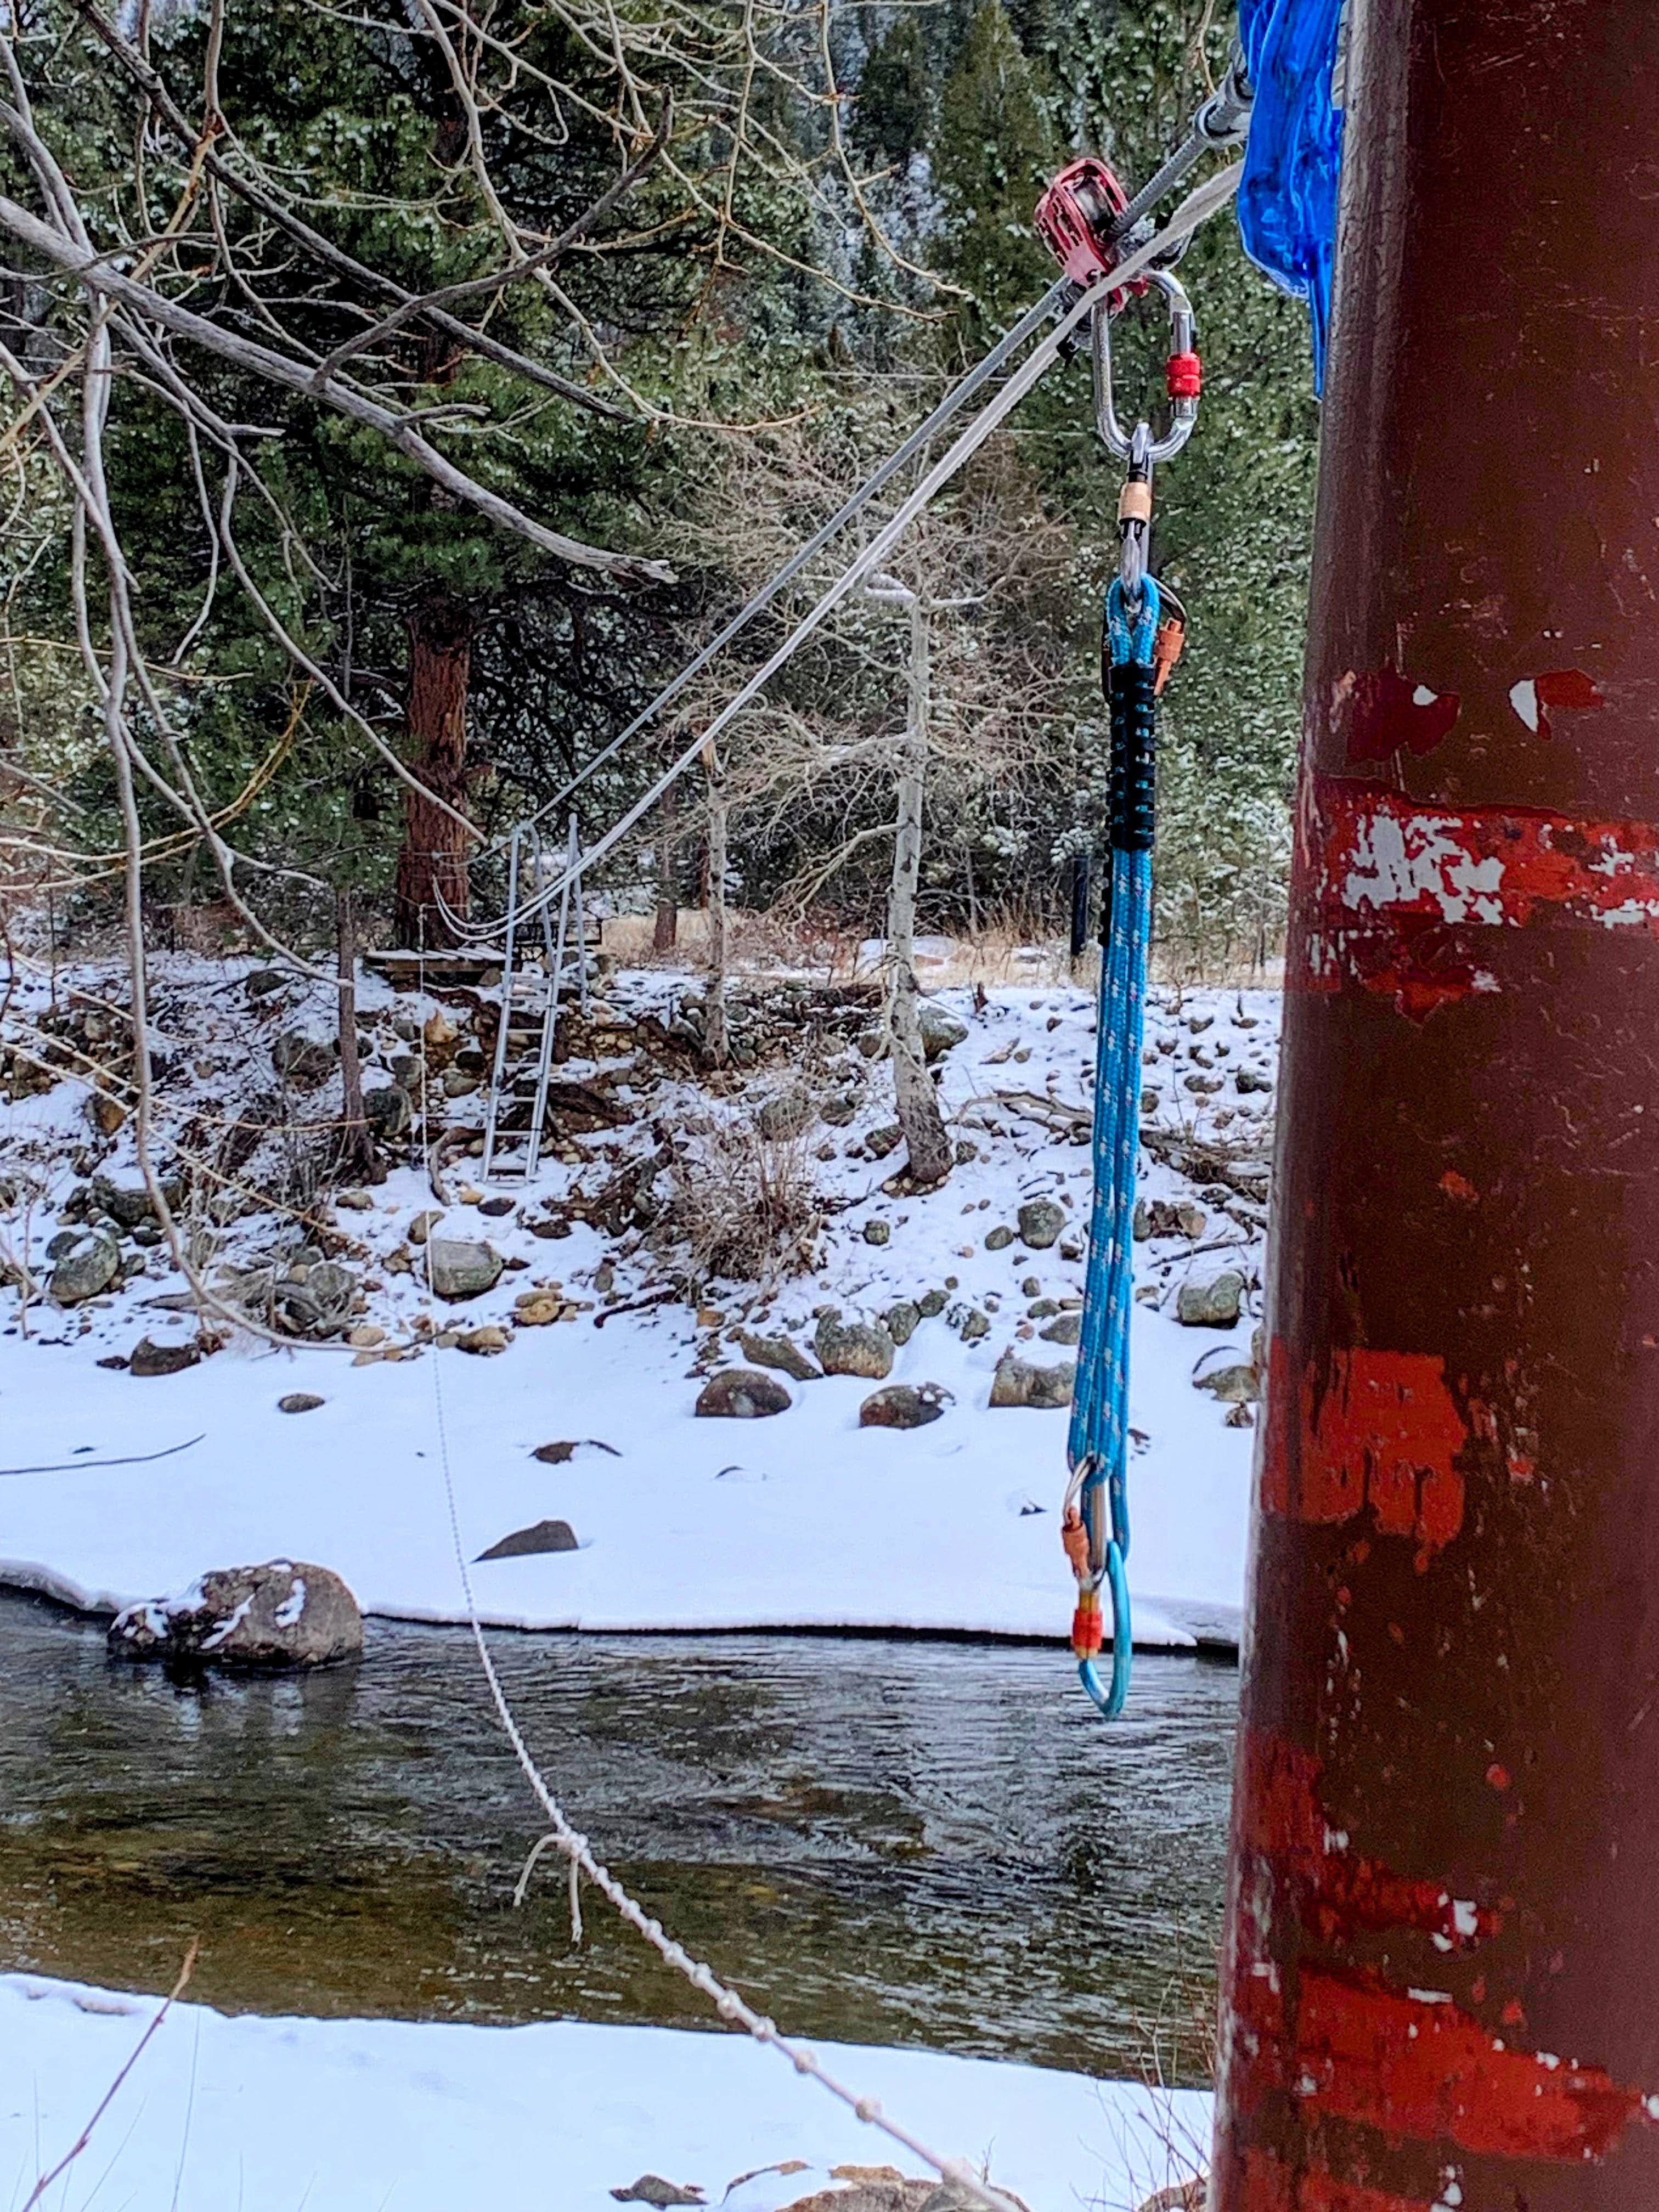
\includegraphics{../Images/zipline} \caption[Zipline]{The homemade zipline stretching across the river fashioned by one of the families who used to live on the other side full time. Photo by author.}\label{fig:figureTitle9}
\end{figure}

Two other families drive over the bridge shared between my family and our two neighbors. They park just on the other side and hike along a rough trail along the river on our land to reach their cabin. Depending on pace and agility, it can take anywhere from fifteen minutes to a half hour, scrambling over two scree fields with large, loose boulders. This was how I got to their cabin when I interviewed them. The majority of homeowners are not physically capable of doing this hike, and some of them have never been able to return to their cabins since their bridge was demolished. When I asked a county official involved in the decision to remove the bridge about introduced public safety hazards to homeowners as a result of removing the bridge, she responded that there wasn't a public safety concern because there were trails to get to the cabins. There is one trail, and not only are most homeowners physically unable to manage it, there are also a limited number of PCFPD volunteers who would be able to make it over the trail. It absolutely increases emergency response time, and it would be logistically complex to have to extract somebody who was physically incapacitated, requiring many hours and the use of the Larimer County Dive Rescue and Search and Rescue, all volunteer teams comprising individuals living primarily in Fort Collins or nearby towns. My own scramble over the rocks for the interview and the hike back out in the waning light of dusk was an embodied experience of the reality of these homeowners, augmented by stories and events accentuating the challenges and risks associated with no longer having easy access to one's home, whether by vehicle or foot. Of the several wildfires which occurred during my fieldwork, one was started across the river and highway from these cabins, embers of which were then whipped up into fire by strong March winds. The wind blew embers across the river, threatening the cabins, which had survived the CPF. In the absence of a bridge, the USFS wildland firefighters were prohibited from crossing the shallow, partially frozen river on foot to reach the other side and had to wait until the Larimer County Dive Rescue team could mobilize in Fort Collins and bring up rafts to ferry the firefighters to the other side, which took several hours. In the end, all the cabins survived, but it was a stark illustration of the consequences of not having a bridge. My participation in different experiences of situatedness through visiting interviewees in their homes was central to cultivating my understanding of the diverse impacts and consequences the CPF and everything it set in motion had for people's lives.

\subsubsection{Poudre Canyon Fire Protection District (PCFPD)}\label{poudre-canyon-fire-protection-district-pcfpd}

I joined the local, rural fire district as a volunteer firefighter for several reasons. First, I wanted to be of service to the community during my fieldwork, and I knew that the fire district always needed volunteers. Second, I anticipated learning a lot about fighting wildfires in the Poudre Canyon and also about how the fire district operates in relation to other agencies, such as the USFS and Larimer County Emergency Services. Third, I knew that the PCFPD had participated in fighting the CPF during its months-long siege, and volunteering for the fire district would allow me to get to know people involved in that work. I continue to volunteer in several capacities, including responding to calls, conducting wildfire risk assessments of homes, and grant administration. My participation with the PCFPD provided a critical perspective on risk governance in relation to multi-jurisdictional hazard response, on the operations of a volunteer fire district in a rural, unincorporated region, and on how the PCFPD responds to various kinds of risk which benefits a much larger geography than the Poudre. I discuss these points in greater detail in Chapter 3 and here provide more information on the composition of the fire district and my role as participant observer.

The district is 99 square miles, its boundary the length of nearly forty miles along the Poudre River and extending two miles wide in some areas. There is much more rural mountainous terrain outside the district whose residents do not have their own district, and the PCFPD is the first responding agency for this additional 150 square miles (\citeproc{ref-Us2024}{{``About {Us}''} 2024}). There are approximately thirty volunteers across four fire stations, two of them in the upper Poudre, one in the lower Poudre, and another outside of and above the canyon, reached by a steep, gravel road with switchbacks from the upper Poudre. Only some of the volunteers respond some of the time, and in the upper Poudre and adjacent area above, only eight respond consistently. Although the residential population of the canyon is quite low, it is a popular recreational area year round but especially in the fall and summer when people visit to fish, hunt, paddle, hike, and backpack in the national forest lands which make up 85\% of the river corridor (\citeproc{ref-CachePoudreWild1990}{{``Cache {La Poudre Wild} and {Scenic River Final Management Plan}''} 1990}). The PCFPD serves a much larger population than actually lives in the canyon. Though only 750-1,500 people live in the entire Poudre Canyon, it receives 500,000-800,000 visitors each year. In 2023, 75\% of the calls were to assist non-residents (\citeproc{ref-PoudreCanyonFire2024}{{``Poudre {Canyon Fire Protection District Newsletter}''} 2024}). The majority of calls to the PCFPD are either medical or vehicle accidents, not wildfires. During the time I have been a volunteer, there have only been three wildfires and three structure fires, out of nearly 200 calls. In addition to emergencies, PCFPD volunteers, including myself, also help with pile burning and wood chipping on private lands to help dispose of woody material called slash that poses a fire danger.

\begin{figure}
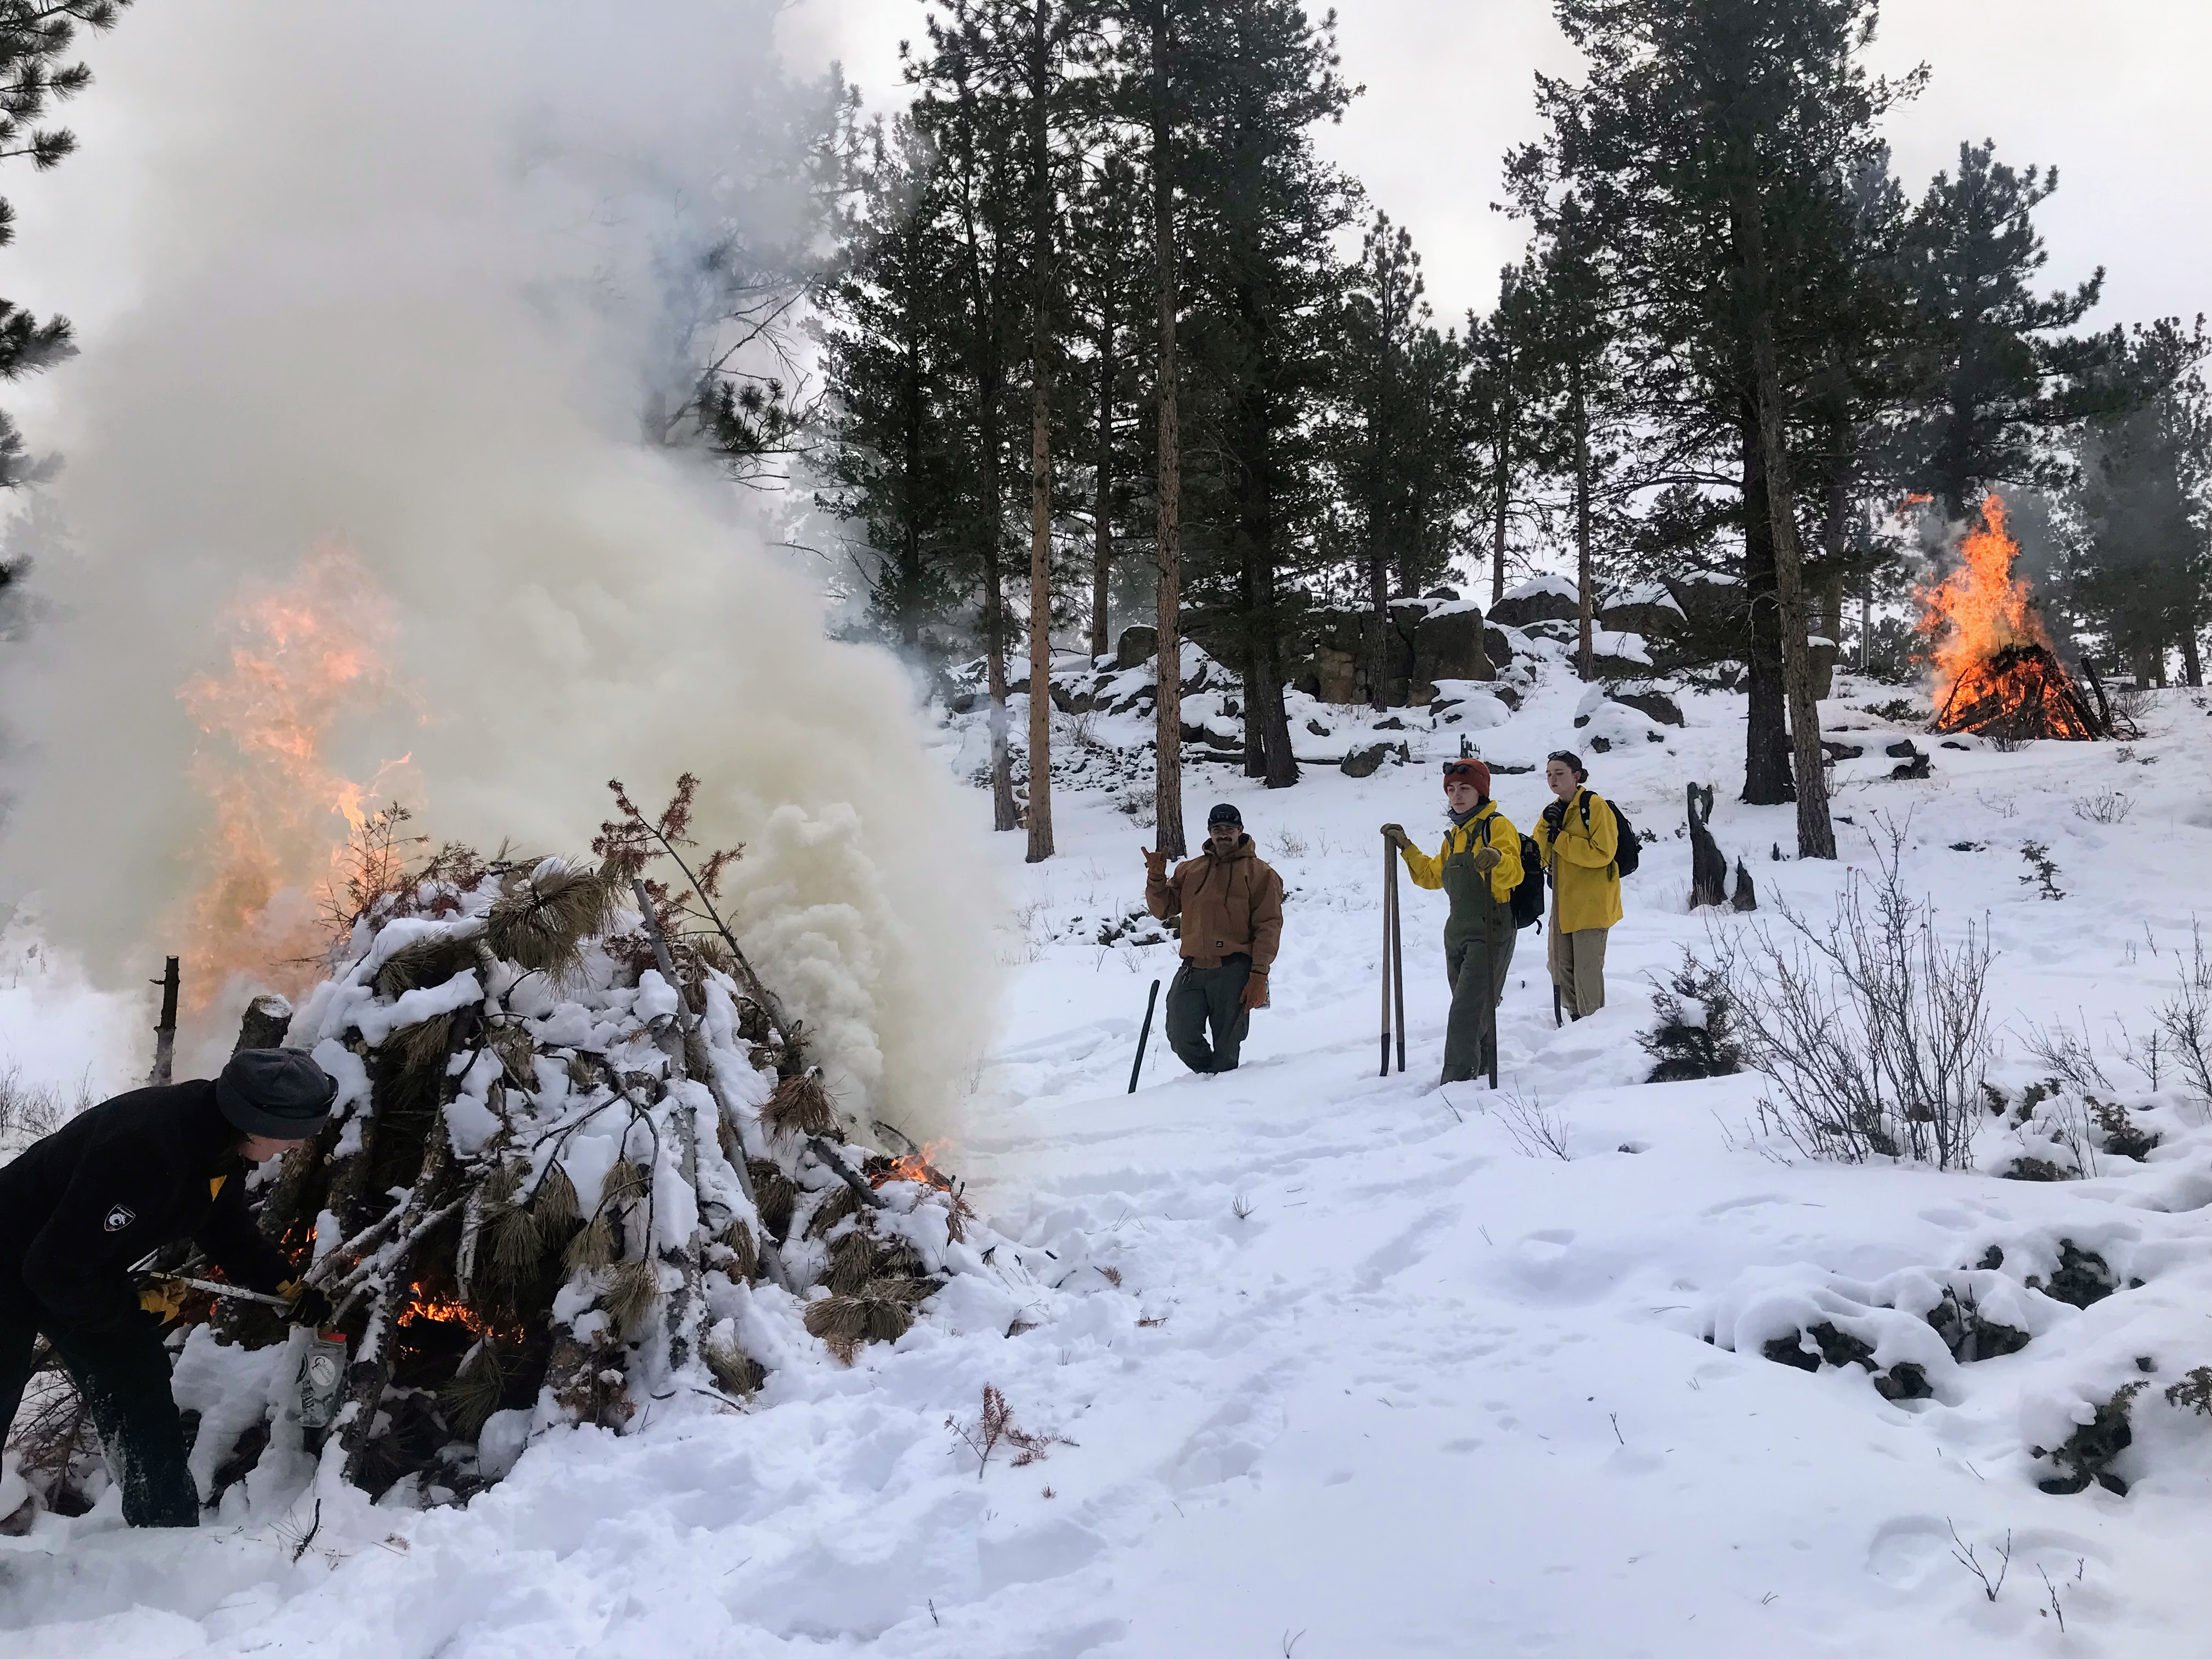
\includegraphics{../Images/burnPile} \caption[Burn piles]{Lighting burn piles at the Ben Delatour Boy Scout Ranch on January 21, 2023. Photo by author.}\label{fig:figureTitle10}
\end{figure}

\paragraph{Multi-jurisdictional Emergency Response}\label{multi-jurisdictional-emergency-response}

Being a volunteer with the fire district situated me within a larger emergency response ecosystem. Certain calls would be beyond our capacity to control, and though we were often the first responders on the scene, we would ask for assistance from other jurisdictions, often Larimer County Emergency Services (LCES), part of the Sheriff's department. In many jurisdictions around the western U.S., the sheriff was originally also designated as the fire marshall by statute. The Sheriff's simultaneous position as chief law enforcement officer as well as Fire Marshall persists uniquely in Larimer County relative to other counties, where the duties of the Sheriff and responding to fire are separated. Those with whom I spoke in Emergency Services seemed to think these dual roles of the Sheriff's department benefited the way they were able to perform their work, without artificially separating different kinds of emergencies. Emergency Management and Emergency Services are separate departments at the county, and only the latter is housed within the Sheriff's office, along with tactical Emergency Medical Services (EMS), SWAT, Hazmat response, and avalanche and swift water rescue. There are seventy-five on-call firefighters. In instances when LCES is called in by the PCFPD to help respond to a medical emergency or to wildland fire, a process referred to as mutual aid, they usually become the Incident Command. The Incident Command System (ICS) is a hierarchical management structure divided into five functional areas to coordinate people and resources for the duration of the incident (\citeproc{ref-u.s.nationalparkserviceWildlandFireIncident2020}{U.S. National Park Service 2020}). The ICS was originally developed to facilitate multi-agency responses to wildfires but is now used across different incidents as part of the National Interagency Incident Management System (NIIMS) (\citeproc{ref-ICSReviewDocument2018}{{``{ICS Review Document}''} 2018}).

My experiences responding to emergencies as a volunteer were sometimes a tragic lesson in what it means to live in a rural, mountainous area with its accompanying risks and hazards, whether wildfire, flooding, car accidents on winding roads with few guardrails, or medical emergencies on UFSS hiking trails. Rural, unincorporated areas rely on volunteer fire departments as the first line of defense against wildfires, as the first responders to accidents and medical emergencies and flooding incidents, rather than dedicated professional emergency services. In the case of the PCFPD, volunteers disproportionately assist visitors compared to residents, frequently under circumstances which occur while driving on state or county roads or recreating on national forest lands. The topography and terrain of the Poudre Canyon and surrounding areas delineate particular hazards that don't exist to the same extent in flatter, less forested areas of Colorado, or the country. The Poudre Canyon, as became apparent during the CPF, facilitates the spread of fire as through a funnel, driven by winds. The water obeys gravity (\citeproc{ref-gordilloGravityPrimacyTerrain2020}{Gordillo 2020}) and flows off the steep mountainsides into the river, which travels down the confines of the canyon walls, restricted by the highway, to the plains below. The plains, however, have their own hazards and sometimes experience worse flooding than the mountains. It is not as if the mountains bear the only measures of risk. However, the relative remoteness of this area, an hour or more away from the closest city, results in real discrepancies in terms of access to services, whether emergency, phone and internet, groceries, technicians, schools, or any other matter of amenities people rely on in their daily lives. And in emergencies, the lack of access to resources is compounded.

\subsection{Research Positionality and Ethical Considerations}\label{research-positionality-and-ethical-considerations}

The essence of my dissertation research is to understand how people living through, researching, and managing the 2020 CPF made sense of both it and its cascading consequences. This research project is rooted in my own experiences of loss and change in a place I have known my whole life and constituted through my experiences and memories. The research process is at times akin to working on a puzzle. Each person I have spoken with about their experiences or perspectives helps me connect another piece, though it may always be an incomplete puzzle. Each piece added to the puzzle reveals more of the larger picture. Sensemaking in a post-disaster context, both the act of gaining understanding, and the sensory engagement of place, is a way of connecting memory and identity tied to past associations with a present and reformulated identity and sense of belonging (\citeproc{ref-moultonHowRememberInterplay2015}{Moulton 2015}).

Although this is not strictly an autoethnographic research project, my personal experiences with the wildfire, accompanying landscape changes, and the ensuing institutional processes of recovery unavoidably shape the outline of my inquiry. I join other disaster anthropologists who started off studying something else and then shifted to focusing on disasters as a result of either personal experiences with disaster or disasters occurring at their field sites (\citeproc{ref-barriosResilienceCommentaryVantage2016}{Barrios 2016}; \citeproc{ref-shneidermanEquivocatingHousesKinship2024}{Shneiderman 2024}; \citeproc{ref-hoffmanWorstTimesBest2019}{Hoffman 2019}; \citeproc{ref-oliver-smithAnthropologicalResearchHazards1996}{Oliver-Smith 1996}).

While certainly not new, anthropology that is autoethnographically informed raises important questions of reflexivity, alterity, and the production of anthropological knowledge. Following other scholars who have contemplated the tensions between subjectivity and objectivity in knowledge production (\citeproc{ref-gibbAnthropologistUndone2005}{Gibb 2005}; \citeproc{ref-navaro-yashinAffectiveSpacesMelancholic2009}{Navaro-Yashin 2009}), I understand ``ethnographic truth'' to be ``partial, perspectival, and embedded in social material relations of power and obligation'' (\citeproc{ref-finnWallsBridgesCultural2000}{Finn 2000}: 140). Further, as the anthropologist Ato Quayson points out, ``alienation is a primary means by which the ethnographer is kept alert to the modes by which he or she theorizes the cultural encounter,'' the experiences of which form the basis for participant observation. In this research, which is also personal, I needed to be aware of the risk of hierarchizing certain knowledges and feelings, and ``rigorously conscious'' (\citeproc{ref-quaysonCalibrationsReadingSocial2003}{Quayson 2003}: 29) of my assumptions. This meant that I had to constantly recalibrate and engage with the experience of alienation in a familiar, now not-so-familiar, landscape and culture.

One way of approaching ethnography in which the researcher becomes affected, as I have been by my experiences of the fire and by the associated loss, requires accommodating a ``form of split experience'' (\citeproc{ref-favret-saadaBeingAffected2012}{Favret-Saada 2012}: 443). Another way is to apply a particular conceptualization of alienation to my research approach --- the alienation effect --- as theorized by Bertolt Brecht who used this phrase to characterize the process of drawing the attention of a theatre audience toward something familiar in order to see it in a new and critical light (\citeproc{ref-brechtBertoltBrechtJournals2020}{Brecht 2020}: 81). The wildfire serves as an alienation effect, causing me to view, experience, and interrogate the social and environmental landscape histories of the Poudre Canyon in an entirely different way, one that lays out a path for an anthropological inquiry.

My own experiences with the 2020 CPF positions me as an anthropologist with an insider perspective of the impacts of wildfires on senses of place, identity, and belonging. It also offers me insight into the complex institutional recovery processes associated with insurance claims alongside county, state, and federal response mechanisms as my family continues to navigate these processes. My closeness to this ongoing disaster has both positive and negative implications and is in itself an ethical consideration. My insider knowledge of the various actors and governing structures provide considerable insight into processes about which I might be otherwise unaware or simply observing. Various aspects of my identity have lent credibility to my role within the community, beyond experiencing loss due to the wildfire, such as my own family's long presence in the Poudre Canyon or my role as a volunteer with the PCFPD.

Throughout my fieldwork, I became more aware of how my experiences, emotional attachments, and political opinions may lead to unwitting bias in my communications with community members or government officials. As a researcher, landowner, and volunteer firefighter, I frequently found myself wearing multiple hats, which required that I make space for a number of different perspectives, both within myself and in relation to others. Wearing multiple hats as a researcher, or occupying ``multiple role relationships'' (\citeproc{ref-collinsCommunitybasedParticipatoryResearch2018}{Collins et al. 2018}) is a common phenomenon in qualitative research (\citeproc{ref-raheimResearcherResearchedRelationship2016}{Råheim et al. 2016}) writ large and in public anthropology (\citeproc{ref-irvinePublicAnthropologyField2012}{Irvine 2012}), critical ethnography, and applied anthropology (\citeproc{ref-ryderCriticalEthnographyResearch2021}{Ryder 2021}) more specifically. This is in part because researchers in these subdisciplines are often acting in service to the communities in which they are conducting their research. Volunteering or playing a specific role in a community beyond just that of a researcher is also a way to engage participants in ways that transcend transactional relationships (\citeproc{ref-ryderCriticalEthnographyResearch2021}{Ryder 2021}) and create a foundation for longer term engagement that goes beyond the fieldwork period. A researcher who has a number of different roles in a community, similar to a researcher engaging in autoethnography, requires careful consideration of positionality and a willingness to be self-reflexive.

My own plural positionalities were brought to my attention most clearly when I attended the Colorado Wildland Fire Conference in April 2023. Many of the people in attendance were fire practitioners, meaning they are members of nonprofits or county, state, or federal agencies working on wildfire prevention, fuels treatments --- meaning some combination of forest thinning and prescribed fire --- and providing homeowners with information about making their homes less susceptible to burning down because of a wildfire, among other things. As a researcher, and as a practitioner of sorts, it was interesting to be exposed to the world of practitioners and managers and to the ways in which they are all versed in the same way of speaking. As a landowner --- and as a researcher --- I sometimes felt like a fly on a wall.

Attending this particular conference, which was the first of several wildfire, climate, or hazard-related conferences I attended in the state, taught me that in Colorado, the world of people who work in wildfire risk reduction, management, and watershed recovery is a small, intimate network of people. This is a testament to the successful collaborations formed by agencies and organizations operating within different jurisdictions. It was also an indication that I needed to be sensitive to the closeness of these relationships among professionals in my research and interviews, although I put my foot in my mouth more than once.

By way of example, before I arrived in Colorado, I virtually attended a meeting in a nearby community to listen in on a discussion of the results of a Community Wildfire Protection Plan (CWPP). I came away with the impression that the young facilitator (from a nonprofit which had helped put together the CWPP) who lives in the city (Fort Collins) was patronizing toward a primarily retirement-age crowd who live in an area considered the wildland urban interface (WUI), a term I problematize in Chapter 3. The WUI is considered the area where development interfaces with fire-adapted landscapes. There are many reasons why the term WUI is problematic, which I detail in Chapter 3, but given its widespread use in fire practitioner worlds and in the literature about wildfire risk (\citeproc{ref-vaskeSalientValueSimilarity2007}{Vaske and Absher 2007}; \citeproc{ref-weiEstimatingWUIExposure2023}{Wei et al. 2023}), there are surprisingly few critiques of the concept and term. This fact is emblematic of how narratives about wildfire and the communities who are exposed to wildfire risk are entrenched and discursively regurgitated by practitioners, managers, and scientists alike. A retired social scientist with the U.S.F.S. is one of few if not the only researcher publicly critiquing the WUI and its underlying assumptions, one of which is a tacit judgement of those who choose to live in areas where wildfires can occur. ``Where are people supposed to live then?'' is one question she poses (\citeproc{ref-mccaffreyFireNarrativesAre2018a}{S. McCaffrey 2018}), considering how many landscapes in the U.S. are fire-adapted, the presence of different kinds of hazards in nearly every place people live, and the complex reasons people live where they do. This meeting I observed was one of the first times I heard the language of ``personal responsibility'' being used in practice, by which I mean the facilitator communicated to the older crowd of people that they needed to take responsibility for living in an area with wildfire risk in the context of implementing the action items to reduce risk identified in the CWPP. I wanted to further examine this set of relations between institutionalized risk reduction and communities as a researcher --- which I do in Chapter 3 --- but I also bristled at the condescension I perceived as a landowner in the WUI. Months later, after I had begun my fieldwork in Colorado, I met with two representatives of another nonprofit and in the context of our conversation about CWPPs, I mentioned the patronizing dynamic between facilitator and the community I had observed. I realized shortly after this, after attending the aforementioned conference, that these two nonprofits were closely aligned and that all the individuals in question work closely together. This was one of many uncomfortable experiences learning how to settle into my multiple roles and coming to terms with my positionality in conducting research for this project. My position is unique because of the personal ways I am connected to my research topic, and the complex ways I simultaneously occupy insider and outsider roles.

\paragraph{Interviews And Other Forms of Data Collection}\label{interviews-and-other-forms-of-data-collection}

Social, economic, and emotional losses due to wildfires, forest management, wildfire policies, and climate change are all emotionally laden topics and at the same time, deeply political. I was sensitive to how people may have felt discussing wildfire policy and governance with a researcher --- and landowner, for that matter --- although I heard no indication of concern from participants. I sought consent from each participant using consent forms, in compliance with the requirements of the UBC Behavioral Research Ethics Board (\# H22-01084). Most people signed the consent forms, while some of those I interviewed over Zoom opted to provide verbal consent instead. Of the fifty interviews I conducted, only two people opted not to be recorded, although due to technical issues with the recorder or disruptive background noise, a total of six interviews were not recorded. Throughout this dissertation, I have only used pseudonyms where I refer to people by name. Although only two people I interviewed explicitly wished to remain anonymous, I chose not to use real names because of the political nature of wildfire governance and recovery, the closeness of the different actors involved (especially scientists and practitioners), and because I hope my research will be published in journal articles aimed at diverse audiences, some of whom would recognize each other if named. It felt more ethical to maintain anonymity for all these reasons.

Another situation that required transparency around collecting information was when I was the convener of an activity. This included two community tours and invited presentations. As a UBC Public Scholar, I was fortunate to receive additional funding from the Climate Emergency Fund (CEF). The purpose of this funding was separate from the goals of my research and was focused on facilitating community discussions related to hazards, some of which had been introduced by the wildfire and some of which were pre-existing. Using this funding, I organized community presentations by four speakers, three fluvial geomorphologists , a forest ecologist, and a local amateur historian. Their presentations functioned as a form of facilitated, collective sensemaking, or at least this was my intention in bringing in experts to speak about their research in wildfire, the study of streams and rivers, or their work in mitigating flooding.

In August 2023, I organized The Future of Forest Service Fuels Treatments Tour with the help of a Fire Management Planning Specialist with the Arapaho-Roosevelt National Forest --- the name of the national forest in the Poudre Canyon and surrounding areas --- a representative from The Ember Alliance, a nationwide nonprofit focused on community planning for wildfires; and the Larimer Conservation District, one of 74 conservation districts in Colorado. I later joined the Board of Directors of The Ember Alliance.

\begin{figure}
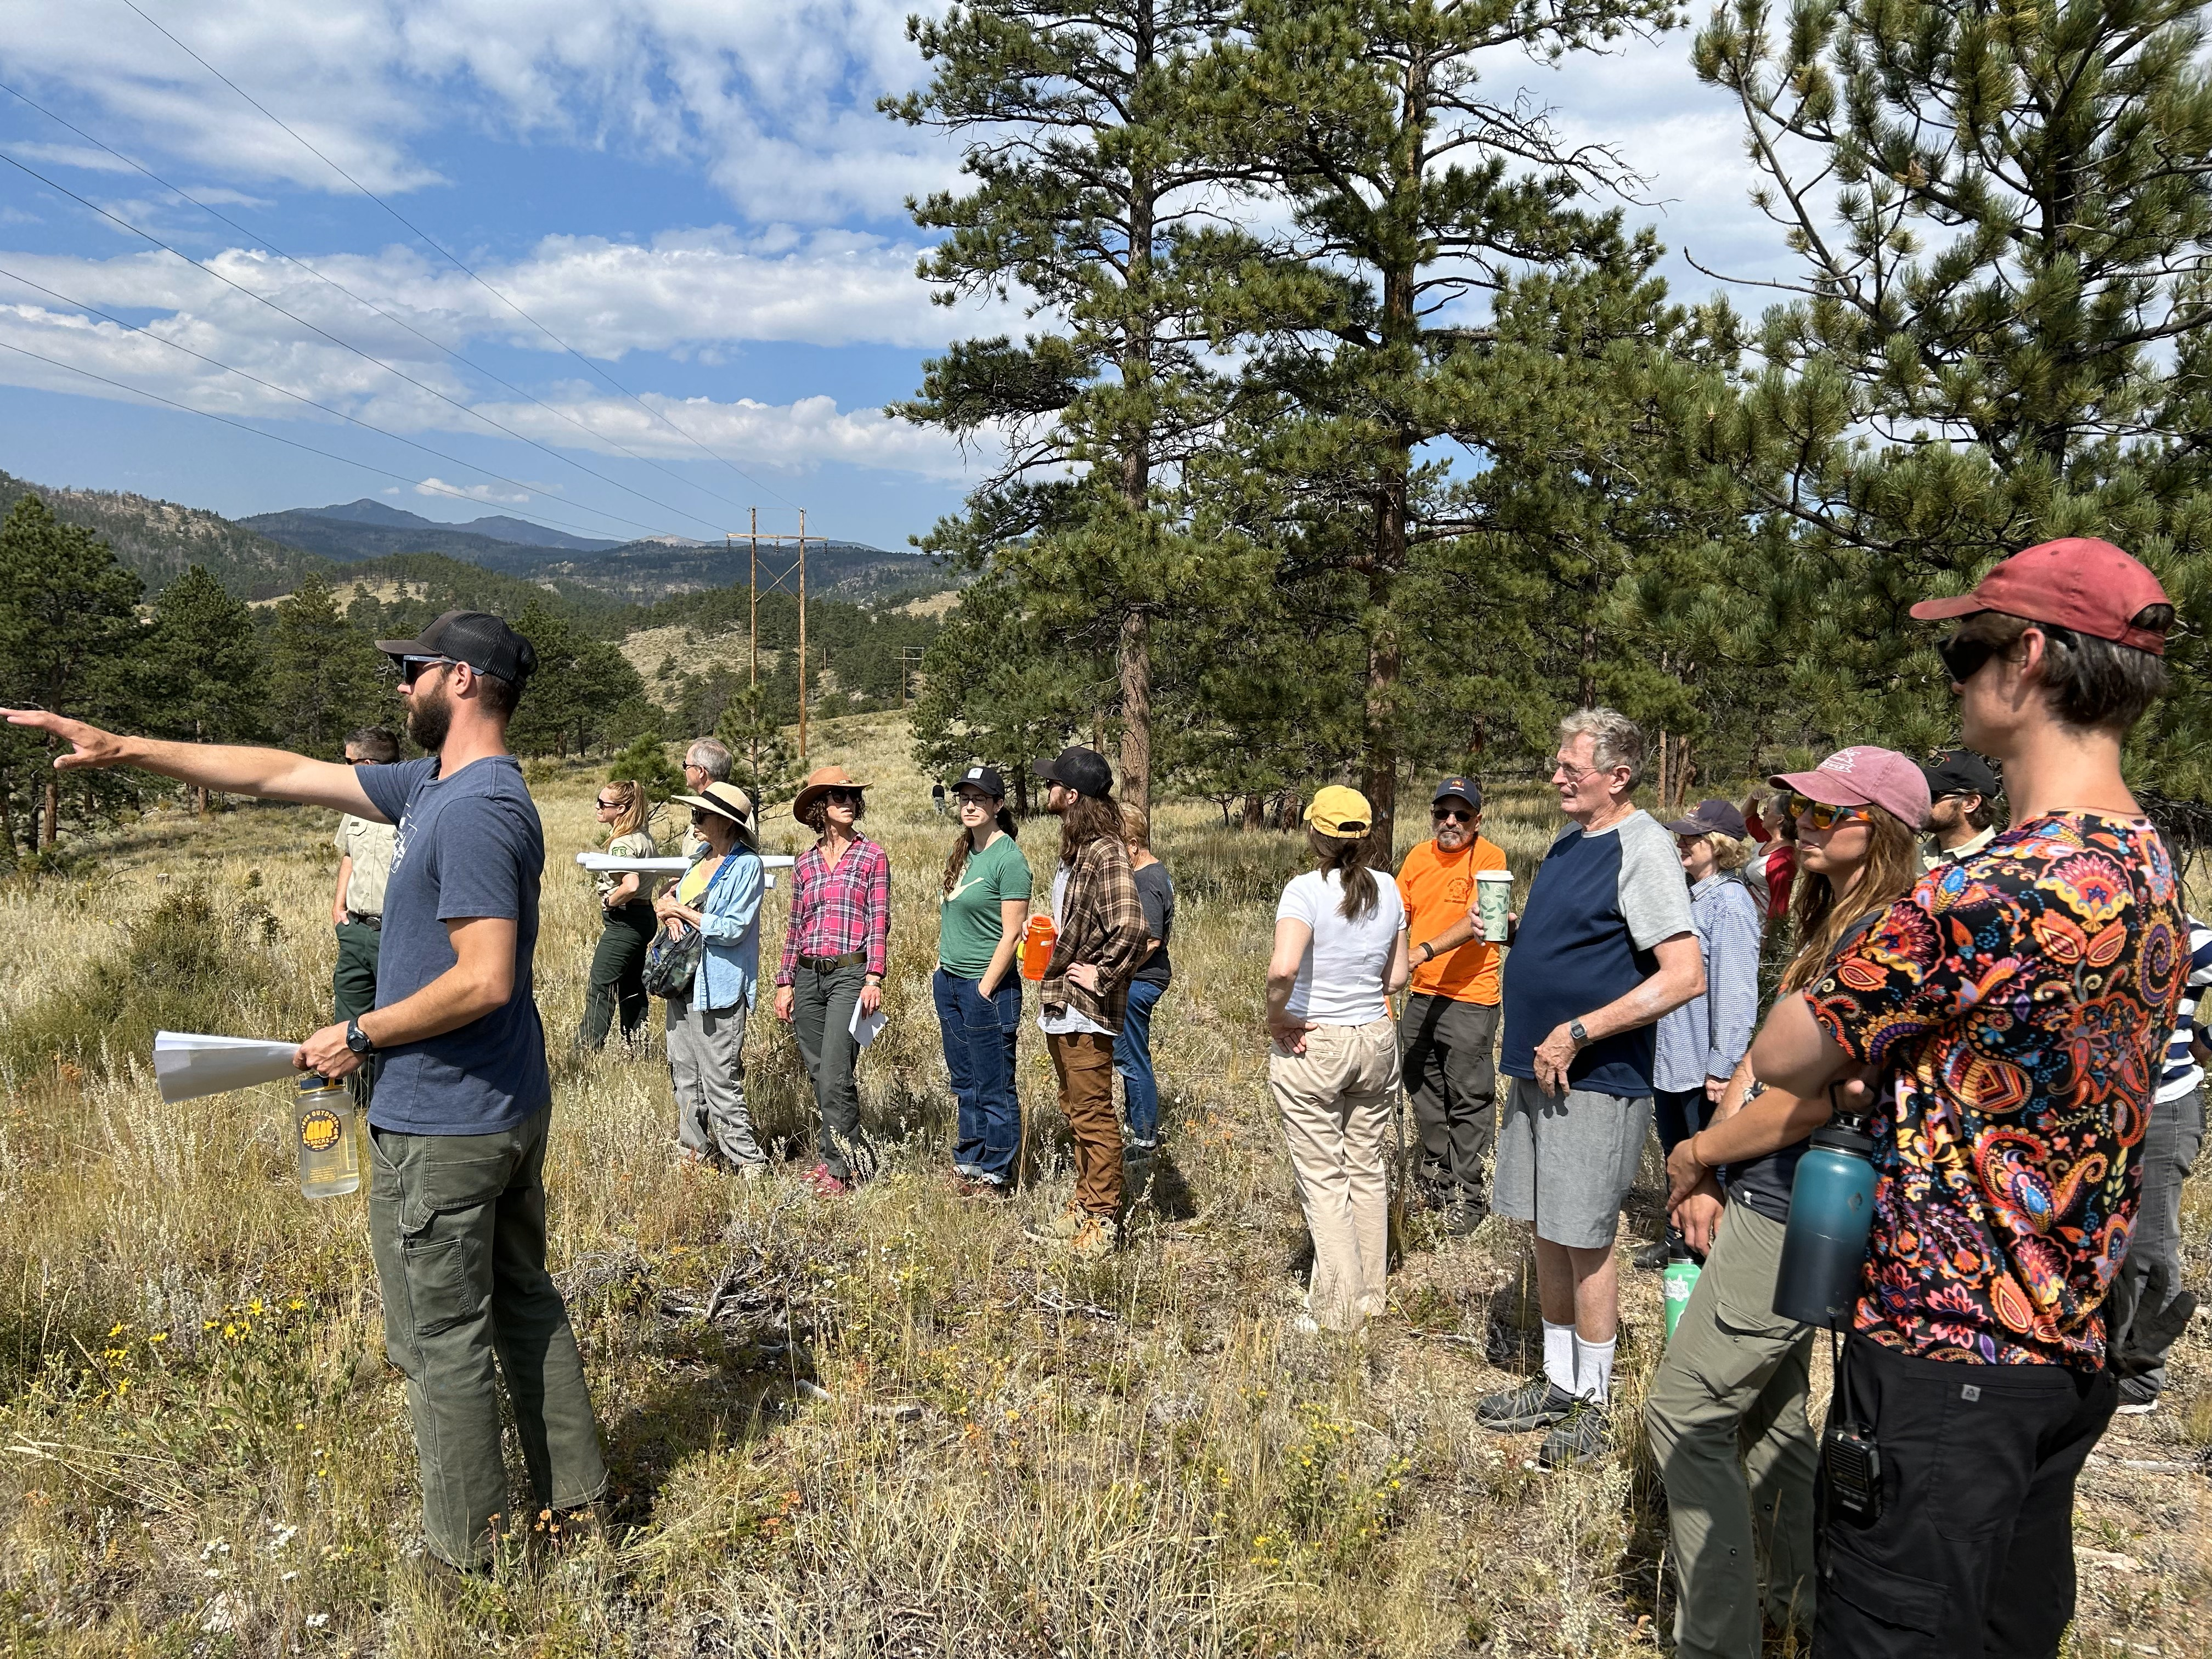
\includegraphics{../Images/fuelsTour} \caption[Fuels treatments tour]{The Future of Forest Service Fuels Treatment Tour. Photo by author.}\label{fig:figureTitle11}
\end{figure}

I also coordinated a Post-Wildfire Flooding Tour for community members in September 2023, facilitated by a fluvial geomorphologist with a consulting firm who had designed all of the flood mitigation structures we visited. The purpose of these tours were twofold. First, I wanted to provide an opportunity to community members who had not directly experienced flooding to visit other community members' homes to see firsthand how flooding or debris flows were impacting them or altering the environment around their homes, led by the person who had designed flood mitigation at all of these sites.

Second, from my position of access as a researcher, I wanted to facilitate relationship building opportunities between community members and representatives from the USFS, the largest landowner in the canyon. Residents of the Poudre live on parcels of private lands surrounded by federal land (and some state), and this arrangement informs the way people perceive the USFS and its management of forests and the river, or inactions. For complicated reasons, the USFS is largely an invisible ``feudal landlord'' (a term borrowed from a presentation by landscape architect Jacob Heydorn Gorski who quoted a community member from a nearby area referring to the USFS). Most USFS employees live in Fort Collins even if they physically work on the Forest, and there are few opportunities for interaction with community members, especially among those employees implementing wildfire-related plans. The USFS has a working relationship with the PCFPD, and leadership in the fire district is more familiar with their activities relative to the rest of the community because they are frequently notified of them. If the USFS is doing a prescribed burn, for example, it will let PCFPD know in case the district receives calls about wildfire smoke. Of the community members on the fuels treatments tour, only those who are members of the PCFPD had prior knowledge of the two treatments we visited. Of course these convening activities were relevant for my research, even if they were organized with different objectives, and required careful consideration in terms of how I engaged with some of the material and people with whom my research brought me into contact.

\subsection{Chapter Overview}\label{chapter-overview}

The following three chapters are structured as standalone journal articles, in various stages of submission. Each of the three chapters contains its own literature review, although I have chosen to compile each chapter's bibliography into one, appearing at the end of the dissertation.

In Chapter 2, I draw on the geological concept of cascading hazards and the ecological concept of a disturbance cascade to highlight how people and landscapes in the Poudre Canyon are concurrently subject to cascading impacts during and after a wildfire. Based on the lived experiences of those in the Poudre and nearby areas, I reflect on the ways people are affected by wildfire that is not easily enumerated and therefore less visible to the public and entities involved in recovery.

I discuss what it means to live with fire in Chapter 3 and show how political conceptualizations of those who live in fire-adapted landscapes are misguided. Drawing on examples from the Poudre Canyon, I demonstrate that people in rural, unincorporated communities exposed to wildfire risk are potential stewards of their communities and the environments in which they live, and play important roles in responding to hazards. In the case of the Poudre, different forms of hazard mitigation at the community level benefits not only residents but also the hundreds of thousands of visitors to the canyon each year as well as water users in populous cities downstream.

In Chapter 4, I describe how community members, practitioners, and scientists go through various stages of sensemaking in response to the CPF and other extreme wildfires. I draw generously on the words of participants themselves to underscore how sensemaking helps recalibrate understandings of risk, agency, control, and impermanence in relation to the forces of fire and flood. Using long-form quotations, I show how recalibration as a result of sensemaking is remarkably similar across the three interview groups. A recalibrated understanding of wildfire and flooding rooted in an appreciation of these phenomena as ecologically integral to the lifecycles and timescales of the material formations of the Poudre Canyon seems to lead to a level of acceptance of wildfire, even of its most destructive forces.

Finally, in Chapter 5, I reflect on my research questions and the findings highlighted in the previous three chapters and discuss how this dissertation contributes to the literatures on landscape, temporality, materiality, and disaster in which I situate my work. I write about the implications of this research project for policy and for helping society navigate extreme wildfire and its cascading impacts. I also discuss the limitations of my dissertation and make suggestions for further research.

\section{References}\label{references}

\clearpage

\section{Cascading Hazards, Cascading Consequences: Linking social-ecological systems in post-fire recovery}\label{cascading-hazards-cascading-consequences-linking-social-ecological-systems-in-post-fire-recovery}

\renewcommand{\thefigure}{2.\arabic{figure}}
\setcounter{figure}{0}
\renewcommand{\thetable}{2.\arabic{table}}
\setcounter{table}{0}
\renewcommand{\theequation}{2.\arabic{equation}}
\setcounter{equation}{0}

\subsection{Introduction}\label{introduction-1}

Dale had just made himself a drink on the afternoon of July 20, 2021, when the power blinked on and off, and he heard what sounded like a shotgun blast. He later attributed the sound to the destruction of an electricity transformer. He looked outside to see a power pole swinging back and forth even though there was no wind and then noticed his patio was covered in about a foot-and-a-half of mud and water. As he futilely tried to get his patio chairs out of the way, all he could think was, `Where is all this water coming from?' He put his rubber boots on and made his way up through the water to what he calls `the shelf,' a flat area on a hill overlooking Black Hollow Creek which flows by the home his father built.

The creek had grown exponentially in size and volume and created a new channel. He watched in disbelief as one of his neighbor's homes floated away down the river. There were four people inside that home, all of whom died that day. Five other homes were destroyed, no vehicles could cross the bridge over the river for a week, and the land on which the remaining homes stood had been radically altered by the mass of trees and huge boulders deposited where houses used to be. These homes and the area immediately surrounding them at Black Hollow, as the settlement is known, had been spared in the 2020 Cameron Peak Fire (CPF). But it became a place of destruction and tragedy more than six months after the fire had been declared contained due to a massive debris flow, a phenomenon closely linked to wildfire as an ecological disturbance.

Wildfire can change the hydrological conditions of a watershed in ways that make it more susceptible to flooding or debris flows, in what is known as a cascading hazard (\citeproc{ref-hydeUncertaintiesPredictingDebris2016}{Hyde, Riley, and Stoof 2016}). Based on my research in a community affected by the CPF, I show how cascading hazards have cascading consequences for people's lives and social structures writ large. I argue that drawing on existing ecological frameworks of the wildfire-flood disturbance cascade to interrogate the wildfire-social disturbance cascade enables the possibility of responding to wildfire in a way that explicitly links social-ecological systems. I propose that cross-disciplinary teams examine post-fire social-ecological conditions and conduct assessments over longer timescales to help coordinate long-term recovery efforts in response to cascading social and ecological consequences.

In geology, cascading hazards refer to a sequencing of processes, beginning with a primary hazard which precipitates the formation of additional hazards (\citeproc{ref-sharmaIncreasingRiskCascading2023}{Sharma et al. 2023}). This is also sometimes called a disturbance cascade (\citeproc{ref-nakamuraDisturbanceRegimesStream2000}{Nakamura, Swanson, and Wondzell 2000}). One example of an ecological disturbance with additional hazard potential, and the one germane to the subject of this paper, is a wildfire which leads to post-wildfire flooding and debris flows. In 2020, a year of record-breaking wildfire activity across the western United States (\citeproc{ref-rodmanHistoric2020Fire2022}{Kyle C. Rodman et al. 2022}), the CPF funneled through the upper Poudre Canyon in northern Colorado on two days of extreme fire spread. This was followed by extensive flooding and debris flows in the summers of 2021, 2022, and 2023, including at Black Hollow.

The physical damage wrought by these intersecting disasters is well documented, and has been quantified in the number of structures destroyed, acres burned, or occurrence of debris flows. The CPF is Colorado's largest wildfire in state history encompassing 208,912 acres (\citeproc{ref-WFIGSInteragencyFire2023}{{``{WFIGS Interagency Fire Perimeters}''} 2023}), which destroyed 492 structures across sixteen communities and three watersheds, including the Poudre, Big Thompson, and Laramie watersheds (\citeproc{ref-coalitionforthepoudreriverwatershedCameronPeakFire}{Coalition for the Poudre River Watershed 2023}). These kinds of statistics appear in research papers (\citeproc{ref-rodmanHistoric2020Fire2022}{Kyle C. Rodman et al. 2022}), on state (\citeproc{ref-HistoricalWildfireInformation2024}{{``Historical {Wildfire Information}''} 2024}) and nonprofit websites (\citeproc{ref-coalitionforthepoudreriverwatershedCameronPeakFire}{Coalition for the Poudre River Watershed 2023}), and in newspaper stories (\citeproc{ref-larsenCameronPeakFire2020}{Larsen 2020}; \citeproc{ref-DeadlyFlashFlood2021}{{``Deadly {Flash Flood Happens Without Notice In Poudre Canyon}, {Resident} '{Never Would Have Believed It}'''} 2021}). As such, numbers become the main way impacts from these hazards are narrated and understood by both the public and government officials. These quantifiable categorizations are typical of most disasters, characterizing them as `temporary aberrations from normal conditions' (\citeproc{ref-fiskeSlowOnsetDisasterClimate2019}{Fiske and Marino 2019, 139}), the idea of which shapes frameworks of disaster response procedures in the U.S. Information about emergency response and recovery is similarly quantitatively understood and measured by, for example, acres burned at high severity, inventories of fish species at risk in burned areas (\citeproc{ref-fairchildFinalFisheriesSpecialist2020}{Fairchild 2020}), or roads most vulnerable to flooding impacts (\citeproc{ref-larimercountyofficeofemergencymanagementCameronPeakFire2021}{Larimer County Office of Emergency Management 2021}). These statistics provide critical information which can be measured against other wildfires and flooding events and offer a sense of both the scale and the number of people or communities who were or are exposed to risk.

Relying primarily on quantitative assessments, however, obscures the varied experiences of contending with multiple hazards, as well as the ongoing ways people's lives continue to be affected, cascading out from the wildfire, for years to come. Quantitative summaries of disaster can also be mobilized by those actors involved in governance who are fluent in the language of risk analysis to produce quantitative risk assessments which not only overshadow non-quantifiable discourses of uncertainty but also hold a strategic advantage in decision-making processes (\citeproc{ref-grovesBombMyBackyard2015}{Groves 2015}).

Disaster anthropologists have shown that disaster survivors are uniquely positioned to reflect on the affective experience of the social and material consequences of disasters (\citeproc{ref-barriosGoverningAffectNeoliberalism2017}{Barrios 2017}; \citeproc{ref-oliver-smithTheorizingVulnerabilityGlobalized2004}{Oliver-Smith 2004}), and the same is true for those who have experienced wildfire and its associated hazards. The complex, sometimes unanticipated, lived experiences of wildfire are important to uncover and interrogate as a way to help better prepare individuals, governments, and society to plan for, respond to, and recover from a series of disasters propagating out beyond the start and end dates of the wildfire itself.

I suggest that in the context of the CPF, and arguably, in the context of most wildfires, there are ongoing and complex consequences for people's lives which cannot be easily enumerated and are therefore not as visible to nor considered by the public, policymakers, and fire and emergency managers. How do we account for, acknowledge, and respond to the complex circumstances of people's lives which result from living through a wildfire? What does recovery look like when we consider the breadth of experiences and account for longer time horizons in our response mechanisms? Focusing on narratives and perspectives emerging from ethnographic fieldwork in the Poudre Canyon, I harness the concept of cascading hazards to examine the accompanying cascading consequences affecting people in this mountainous area of northern Colorado following the CPF.

This article is organized as follows. First, I propose a conceptual framework of the social-ecological disturbance cascade for responding to wildfires. Second, I provide an overview of the literature on wildfire and disturbance in the social sciences and the anthropological approaches I draw on for this paper. Third, I describe my study site and the specific landscape characteristics which support a social-ecological perspective of disturbance. Fourth, I explain the methods I used for my research and why they are relevant for a landscape perspective of wildfire-related disturbance examining human and more than human relations. Fifth, I present and discuss results showing how cascading hazards resulting from wildfires have cascading consequences for people's lives. Finally, I reflect on the fire and emergency management and policy implications for utilizing a social-ecological disturbance cascade framework and propose one possible strategy for wildfire recovery in the future.

\subsection{Conceptualizing the Social-ecological Disturbance Cascade}\label{conceptualizing-the-social-ecological-disturbance-cascade}

The disturbance cascade involving wildfire and flooding is well known and oft-studied among those who research geological hazards such as landslides and debris flows (\citeproc{ref-rengersLandslidesWildfireInitiation2020}{Rengers et al. 2020}; \citeproc{ref-staleyRecurrenceIntervalPostfire2020}{Staley, Kean, and Rengers 2020}) or fluvial geomorphology, the study of the movement of rivers over time and how they shape landforms (\citeproc{ref-wohlBiogeomorphicInfluencesRiver2022}{Wohl et al. 2022}). Following a wildfire, there is an expectation among the scientific research and watershed management communities that there will be a disturbance cascade (\citeproc{ref-barnardWildfireClimateChange2023}{Barnard et al. 2023}; \citeproc{ref-hohnerWildfiresAlterForest2019}{Hohner et al. 2019}), and that post-fire conditions provide an opportunity to study the particular ways the disturbance cascade is enacted in specific watersheds (\citeproc{ref-gorrTriggeringConditionsRunout2023}{Gorr et al. 2023}), which will vary based on a number of ecological, geomorphological, and anthropogenic factors.

Following the CPF and other large-scale wildfires, researchers have been studying changes to soil microbiome diversity (\citeproc{ref-nelsonWildfiredependentChangesSoil2022}{Nelson et al. 2022}), the relationship between wildfire-induced changes in source water to downstream water supply and agricultural production (\citeproc{ref-barnardWildfireClimateChange2023}{Barnard et al. 2023}), the role of large woody debris in post-fire debris flow sediment retention (\citeproc{ref-rengersInfluenceLargeWoody2023}{Rengers et al. 2023}), analysis of post-fire conditions to guide reforestation management (\citeproc{ref-rodmanHistoric2020Fire2022}{Kyle C. Rodman et al. 2022}), and how spatial heterogeneity in post-fire mountain watersheds influences the transport of sediment downstream (\citeproc{ref-wohlBiogeomorphicInfluencesRiver2022}{Wohl et al. 2022}), among many other projects.

In contrast, in the social sciences, I am aware of only one research project related to community member experiences following CPF (\citeproc{ref-kooistraWebinarResidentsPerspectives2022}{{``Webinar: {Residents}' {Perspectives} on {Colorado}'s 2020 {Cameron Peak Fire}''} 2022}) and one project assessing risk management tools during the fire (\citeproc{ref-caggianoCameronPeakFire2021}{Caggiano et al. 2021}).

There is no commonly used term to describe cascading hazards in the social sciences, even though there is a strong history of social science research on the human dimensions of wildfires, including the recognition of wildfire as having both ecological and social ramifications (\citeproc{ref-tomanSocialScienceWildlandurban2013}{Toman et al. 2013}). I propose the term social-ecological disturbance cascade to delineate the explicit relationship between a wildfire, its ecological disturbance cascade, and the cascading consequences for people's lives it sets in motion. My research demonstrates that communities who suffer ongoing impacts from wildfires often experience them in ways connected to the ecological disturbance cascade and could benefit from an approach that mirrors some watershed-specific, longitudinal studies more common in ecological and geological research and restoration of post-wildfire conditions. Acknowledgement and understanding of social-ecological linkages in disturbances among those in positions of power, who formulate policy, and researchers of all backgrounds conducting wildfire and post-wildfire studies which inform policy and management decisions would stimulate and support more comprehensive future wildfire response and recovery efforts that are sensitive to the complex and ongoing needs of people living in wildfire-impacted areas.

Linking the study of ecological and social disturbance cascades facilitates an understanding of wildfire as a phenomenon shaped by and with implications for both ecological and social forces and enables the possibility of inclusive social-ecological responsiveness. Currently, at the federal level, preparation for and response to wildfire is logistically, financially, and administratively separated from preparations and responses associated with flooding caused by wildfires, and from wildfire smoke. Responsibility for these different phenomena is spread across multiple agencies operating under different mandates and with no clear pathway for cross-agency coordination. Wildfire management, including its prevention or reduction in its severity, is primarily the purview of the U.S. Forest Service (USFS). Wildfire smoke, on the other hand, which inevitably accompanies wildfires but can also be experienced by communities far from the source of the wildfire --- such as the smoke engulfing New York City from Canadian wildfires in 2023 (\citeproc{ref-lowreyNewYorkFailed2023}{Lowrey 2023}) --- is managed by the U.S. Environmental Protection Agency (EPA). Research on post-fire flooding and debris flows is published by the U.S. Geological Survey (USGS), while funding for private property flood mitigation is often routed through the Natural Resource Conservation Service (NRCS), unless it is funded and directed instead under the purview of the Federal Emergency Management Agency (FEMA) in the event of federally declared disasters. States, counties, municipalities, fire districts, and nonprofits all interface with federal agencies in managing wildfire and post-fire watersheds in different ways.

This multi-jurisdictional but disunited management approach to the multiple hazards associated with wildfire and their implications for human lives results in disjointed preparedness. Readying the space surrounding one's home in order for the house to better withstand a wildfire does not prepare a homeowner to prevent excessive exposure to wildfire smoke. Similarly, post-fire recovery is multifaceted and jurisdictionally complex. Homeowners may be faced with a number of different challenges, including life-threatening flooding, road and bridge access or damage issues, insurance claims, home rebuilding and permitting processes, hazardous trees, slash (woody debris) build-up, emotional and physical distress, infestations of invasive plant and insect species, property damage from bears, rodents, or decomposing food during evacuations and power shut-offs, and reforestation needs. Any one of these issues may be managed alternately by different federal, state, or county agencies or nonprofits or not managed by any jurisdiction at all. There may be resources and funding available for a short period to address certain challenges such as the sandbags provided by the Larimer County Office of Emergency Management (OEM) the first summer following the CPF in 2021 but not for subsequent flooding events in the summers of 2022 and 2023. These challenges may occur simultaneously or years apart from each other, highlighting the need for a pathway to recovery built in response to anticipated and unanticipated, or simply cascading, social-ecological disturbances over multiple timescales and jurisdictions. A pathway which includes funding mechanisms to address wildfire-related preparation, response, and recovery over a longer timeframe, accounts for cross-jurisdictional complexity, and provides a central hub of resources and support would reduce the navigational hurdles with which those confronting multiple hazards over a number of years have to contend.

\subsection{An Overview of Wildfire and Disturbance in the Social Sciences}\label{an-overview-of-wildfire-and-disturbance-in-the-social-sciences}

Earlier and ongoing wildfire-related social science research in anthropology, sociology, geography, and other disciplines across the globe has focused on fire and land management (\citeproc{ref-charnleyDiversityForestManagement2017}{Charnley et al. 2017}; \citeproc{ref-zaharaBreathingFireLandscapes2020}{Zahara 2020}; \citeproc{ref-essenImprovingWildfireManagement2023}{Essen et al. 2023}), wildfire mitigation (\citeproc{ref-mccaffreyUnderstandingWildfireMitigation2020}{S. McCaffrey et al. 2020}; \citeproc{ref-nicoleRiskPerceptionsMitigation2021}{Nicole et al. 2021}; \citeproc{ref-meldrumRethinkingCostsharePrograms2024}{Meldrum et al. 2024}), suppression (\citeproc{ref-calkinNegativeConsequencesPositive2015}{David E. Calkin, Thompson, and Finney 2015}), fuels treatments (\citeproc{ref-mccaffreyPrescribedFireWhat2006}{S. McCaffrey 2006}; \citeproc{ref-millerBarriersEnablersPrescribed2020}{Miller, Field, and Mach 2020}), on risk perceptions related to wildfire (\citeproc{ref-weisshauptNorthernInlandWest2007}{Weisshaupt et al. 2007}; \citeproc{ref-cohnWildlandUrbanInterfaceResidents2007}{Cohn, Williams, and Carroll 2007}), smoke (\citeproc{ref-haglerEditorialUnderstandingCommunicating2021}{Hagler et al. 2021}), and flooding (\citeproc{ref-burnettFactorsInfluencingFlood2023}{Burnett and Edgeley 2023}; \citeproc{ref-calkinHowRiskManagement2014}{David E. Calkin et al. 2014}), wildfire preparedness (\citeproc{ref-mccaffreyCommunityWildfirePreparedness2015}{S. McCaffrey 2015}; \citeproc{ref-jakesImprovingWildfirePreparedness2007}{Jakes et al. 2007}), communication (\citeproc{ref-taylorInformingNetworkImproving2007}{Taylor et al. 2007}; \citeproc{ref-christiansonCanadianWildfireCommunication2011}{Christianson, McGee, and Jardine 2011}; \citeproc{ref-kumagaiCausalReasoningProcesses2004}{Kumagai et al. 2004}), individual and community wellbeing following wildfires (\citeproc{ref-burnsIntegrativeHealingImportance2007}{Burns, Taylor, and Hogan 2007}; \citeproc{ref-carrollFireGalvanizingFragmenting2005}{Carroll et al. 2005}), and considerations for future research in assessing the social impacts of wildfire (\citeproc{ref-paveglioUnderstandingSocialImpact2015}{Paveglio, Brenkert-Smith, et al. 2015}). Among social scientists studying wildfire, there is broad recognition that wildfires have wide-ranging social impacts beyond that which can be captured by statistics. Compared to other disasters such as hurricanes or floods, research on the ways wildfires impact specific communities over time is less common, and ecological consequences may be easier to characterize than social ones (\citeproc{ref-kentSocialEconomicIssues2003}{Kent et al. 2003}).

The concept of disturbance has also previously been leveraged to characterize wildfire impacts on people's lives. A compendium of wildfire-related social science research findings identifies wildfire as a social as well as ecological disturbance with both tangible and intangible impacts for people's lives (\citeproc{ref-tomanSocialScienceWildlandurban2013}{Toman et al. 2013}). Writing more generally about disasters as disturbances, Hodgson advocates for institutionalized sense-making as a pathway for community adaptation to the impacts of disasters (\citeproc{ref-hodgsonEmotionsSenseMaking2007}{Hodgson 2007}).

\paragraph{Anthropological Approaches to Disaster, Landscape, and Time}\label{anthropological-approaches-to-disaster-landscape-and-time}

In spite of multidecadal research related to wildfire across disciplinary fields in the social sciences that has come to inform fire and emergency management strategies, the way we understand, prepare for, and respond to wildfires more generally continues to artificially separate social and ecological disturbances and their consequences over different timescales and across multiple jurisdictions. Anthropological scholarship identifies the temporal inscriptions (\citeproc{ref-adamsMarketsSorrowLabors2013}{Adams 2013}) and social lives of disasters (\citeproc{ref-sorensenSocialLifeDisasters2015}{Sørensen and Albris 2015}), which, through various cultural processes, expand beyond the timeframe and physical perimeter of the disaster itself.

Anthropologists have encouraged the consideration of materialist conceptualizations of time and space (\citeproc{ref-mooreAnthropoceneAnthropologyReconceptualizing2016}{Moore 2016}), particularly in relation to the Anthropocene, the term proposed to signify a new geological epoch characterized by human-driven actions and processes. Whatever criticisms there may be of the term Anthropocene (\citeproc{ref-millingtonHimalayanBuddhismHuman2024}{Millington 2024}), attending to the way human materialities and temporalities intersect with more than human material and temporal formations and processes requires us to conceptualize `an expansive ecology of time' (\citeproc{ref-widgerMonsoonUncertaintiesHydrochemical2020}{Widger and Wickramasinghe 2020}) which transcends a human-centered idea of history (\citeproc{ref-chakrabartyAnthropoceneTime2018}{Chakrabarty 2018}) and the `complex conjunctures' (\citeproc{ref-mooreAnthropoceneAnthropologyReconceptualizing2016}{Moore 2016, 36}) of the spaces of the Anthropocene. Following Tsing and coauthors, who propose that anthropologists engage with landscape to study how human and beyond human relations are structured relative to each other (\citeproc{ref-tsingPatchyAnthropoceneLandscape2019}{A. L. Tsing, Mathews, and Bubandt 2019}), I use the post-wildfire landscape of the Poudre Canyon to understand the conditions of social and ecological disturbances resulting from the CPF and reverberating over time in response to each other. Situated ethnographic fieldwork over longer time horizons more typical in anthropology can illuminate narrative experiences of wildfire and its cascading consequences over time and help make sense of the ways in which these experiences are often connected to or exacerbated by the ecological disturbance cascade.

\subsection{Study site}\label{study-site}

As I describe in this section, the Poudre Canyon constitutes a landscape conducive to cascading geological hazards resulting from wildfire. There are 750 full-time and 1,500 part-time residents (\citeproc{ref-Us2024}{{``About {Us}''} 2024}). The Poudre River parallels Highway 14 in the canyon for approximately forty miles as it flows along the contours of steep, forested slopes and rocky outcrops, supplying water for the hundreds of thousands of people in the populous Front Range cities of Fort Collins and Greeley. The Poudre Canyon's two main population centers are divided between the lower and upper canyon. In 2012, the High Park Fire swept through the lower Poudre and several nearby communities, destroying 259 homes. In 2020, the CPF burned over much of the upper Poudre and fifteen other communities in Colorado over nearly four months. My own family's historic home, and that of our neighbor's, located in the upper Poudre, were the first two houses to burn in the fire, an experience which initiated this research inquiry.

The river corridor itself is made up of 85\% federal lands, with only 2,000 out of 25,000 acres in private ownership (\citeproc{ref-CachePoudreWild1990}{{``Cache {La Poudre Wild} and {Scenic River Final Management Plan}''} 1990}). The lands beyond the corridor are primarily owned by the USFS. Private lands are primarily situated along the river where flatter ground makes it easier to build, hemmed in by the canyon's steep, rocky mountainsides, carved out by a glacier in the uppermost sections of the canyon, or by the river, below the glacier's end moraine. Many, if not all, of these flatter pieces of land were formed either by alluvial fans, an accumulation of sediments that fans outward at the point where a steeper gradient meets a less steep gradient, or because they are part of the river's old floodplain. The Poudre River watershed drains around 1,889 square miles in the canyon alone, although the river continues east as it flows out of the canyon, 125 miles in total until its confluence with the South Platte River on the eastern plains of Colorado. In populated areas of the Poudre, some of the river's thousands of miles of tributaries pass through private lands, often in their lowest reaches before reaching the river. Most early settlers, and where the largest numbers of people continue to be based, built in proximity to a creek and prioritized settling land where they could ranch, mine, or extract timber, which was sent down the river during the years 1868 to 1885 to use as railroad ties (\citeproc{ref-evansCachePoudreNatural1991}{H. E. Evans and Evans 1991}). This topography, formed by thousands of years of geologic movement, combined with land use and ownership established over shorter timescales, help shape the nature of the consequences which people in the Poudre experienced over the course of two large wildfires and in the years following these wildfires.

\begin{figure}
\includegraphics{../Images/watershed} \caption[Cache la Poudre watershed]{The Cache la Poudre watershed. Map by the Coalition for the Poudre River Watershed.}\label{fig:figureTitle12}
\end{figure}

The Poudre is officially composed of three unincorporated communities (\citeproc{ref-LarimerCountyColorado2024}{{``Larimer {County}, {Colorado}''} 2024}). Larimer County, and its Board of County Commissioners with three elected officials, is the defacto governing body for all unincorporated communities, although the Poudre Canyon Fire Protection District (PCFPD) is a local governmental entity whose jurisdiction for emergency response and wildfire management encompasses the entire populated length of the Poudre Canyon (\citeproc{ref-Us2024}{{``About {Us}''} 2024}). Post-CPF recovery coordination was divided geographically in the Poudre Canyon between the City of Greeley, which has water rights to the Poudre River, and Larimer County. City of Greeley coordinated watershed recovery west, or upstream, of a bridge called Crown Point, and Larimer County was responsible for the areas east of this, or downstream.

\subsection{Methods}\label{methods}

I used ethnographic research methods to investigate how cascading hazards resulting from the CPF have cascading consequences for those affected by the wildfire. Ethnography is able to capture the situated, temporal complexities of how humans are affected by wildfires and associated hazards (\citeproc{ref-mcgranahanWhatEthnographyTeaching2015}{\textbf{mcgranahanWhatEthnographyTeaching2015?}}; \citeproc{ref-jusionyteThresholdEmergencyResponders2018}{Jusionyte 2018}).

\subsubsection{Participant Observation}\label{participant-observation}

From June 2022 to October 2024, I lived in the upper Poudre and participated in activities such as social events, community association and fire board meetings, and site visits to private property and USFS lands impacted by wildfire or flooding. I joined the PCFPD as a volunteer and learned about how the fire district operates in relation to other agencies, such as the USFS and Larimer County Emergency Services. I attended conferences on wildland fire and natural hazards, joined educational tours and citizen science initiatives coordinated by local nonprofits, and participated in chipping and burning slash for neighbors.

\subsubsection{Interviews}\label{interviews}

I conducted fifty semi-structured interviews with community members, wildland fire, emergency and watershed management practitioners, and researchers whose studies intersect with ecological, geological, or social aspects of wildfire, post-fire flooding, or recovery. Of these, twelve also included open-ended conversations while walking in the CPF burn scar or accompanying researchers doing scientific fieldwork, a kind of walking interview (\citeproc{ref-evansWalkingInterviewMethodology2011}{J. Evans and Jones 2011}; \citeproc{ref-carpianoComeTakeWalk2009}{Carpiano 2009}). In addition to interviews, I also used the go-along method (\citeproc{ref-kusenbachStreetPhenomenologyGoEthnographic2003}{Kusenbach 2003}) to accompany three different teams of researchers --- fluvial geomorphologists, biogeochemists, and geologists --- in four wildfire-impacted watersheds during their fieldwork, and seven scientists and fire/watershed managers within areas of the CPF burn perimeter. I identified participants by meeting them at community events, conferences, and other events, through literature reviews, and snowball sampling.

My premise, reflected in the experiences of those I interviewed and the conditions I observed, is that wildfire initiates a series of ongoing, cascading impacts on people's lives, captured through sustained research presence and engagement with community and expressed through narratives.

\subsection{Categories of Consequences}\label{categories-of-consequences}

In this section, I examine the different social consequences emerging from the 2020 CPF in the upper Poudre Canyon, showing that 1) social impacts on people's lives can be categorized to capture the broad range of cascading experiences resulting from the original disturbance of the wildfire; 2) while social and ecological disturbances can occur in a kind of feedback loop, tracing ecological disturbances can help us anticipate social ones; and 3) the social-ecological disturbance cascade will be different for each community affected by wildfire but can be used to inform future scenarios for communities which have not yet experienced wildfire.

According to the measures typically used to account for how destructive a wildfire is, the upper Poudre fared reasonably well. Of the 492 structures destroyed in CPF, which lasted for 112 days, fewer than twenty were in the upper Poudre, which was the closest community to the wildfire and experienced two days of rapid fire growth over a month apart, affecting different sides of the canyon. Of the structures lost in the Poudre, none were primary homes, nobody died in the wildfire, including firefighters, even though it occurred during the COVID-19 pandemic, which complicated firefighting efforts and evacuations. These numbers, while important, do not contain within them the many ways people's lives were disrupted by the wildfire that are essential for thinking through how to help other communities in the future respond to and recover from wildfire. Below, I provide some examples of social disturbance cascades, many of them linked to disturbances on the landscape.

\subsubsection{During the Fire}\label{during-the-fire}

One couple in the upper Poudre was evacuated from their home the day the fire started just after stocking their refrigerator with groceries from Fort Collins. They were only able to return to their property seventy-three days later, after living in a hotel room with two cats. By the time they were permitted to return home, they had to replace their kitchen floor and their refrigerator on account of the food which had melted and rotted onto the floor when the power was shut off. One of their neighbors fared worse because his home was broken into multiple times by a bear who smelled the decomposing food and wreaked havoc throughout the house. The damage was so extensive he had to hire a contractor, who turned out to be corrupt. When I interviewed the neighbor about his experiences, he said:

\begin{quote}
You know, in a lot of ways, the fire was the end at the same time that the fire was the beginning. It's tough when I think about it and I get emotional still, I get very upset. What I grew up with and what was inculcated into my being about the woods and the wilderness and the animals and the views and a sense of belonging to all that. The fire ended that. And while I'm appreciative of the little oasis, I'm still devastated when I drive through the burn scar. So the fire was the end. But then the fire is also the beginning, like the forest floor coming back and wildlife returning. But it also was the beginning, the catalyst for all these subsequent events. The bear wouldn't have been in here if the fire hadn't burned through, and he wasn't distressed and hungry. If I hadn't evacuated and stuffed everything in the freezer thinking I'm gonna be back in a few days. And then the power gets shut off, and all of a sudden the cabin reeks, and he has a smorgasbord for four days. Never would have happened. If that hadn't happened, I never would have had to hire this jackass of a contractor. And he wouldn't have destroyed my house and done more damage than the bear did.
\end{quote}

Under normal circumstances, the presence of wildlife is often awe-inspiring for Poudre Canyon residents and one of the reasons people enjoy living there. During and in the years since the wildfire, however, residents have encountered some animals in unusual ways: multiple break-ins from bears, sometimes at strange times, like the night of the Black Hollow debris flow in one of the surviving homes; extreme mice infestations in a home evacuated for a short time; packrats which had previously nested in a workshop which burned down moved into the house which survived; and a black widow infestation where none of these spiders had been seen before over multiple generations. Some of these impacts are short-lived, like the mice infestation, whereas others are persistent, like the packrat nests. These multispecies encounters (\citeproc{ref-ogdenAnimalsPlantsPeople2013}{Ogden, Hall, and Tanita 2013}), in their myriad forms, are one of the unaccounted-for categories of the consequences of wildfire.

It is worth noting that when it comes to people's interactions with wildlife following the wildfire, not all have been negative. In the summer of 2023, an ecologist pointed out mating Lewis's Woodpeckers on my family's land in an area she said they would not have found habitat before the fire. Two people interviewed in 2023 observed that wildlife seems to be thriving after the wildfire based on their observations, more twin moose calves and fawns and more abundant and diverse wildlife sightings in general. This may point to another kind of opening when we connect social and ecological circumstances in examining wildfire's impacts. People's experiences and perceptions of ecological conditions in the Poudre help shape how they make sense of wildfire, of a changed and changing landscape, of the beginnings and ends of things and how they feel about them.

\subsubsection{After the Fire}\label{after-the-fire}

For the people who did lose homes or other buildings to the wildfire, it set in motion its own series of cascading impacts, which are specific to this experience, in the form of loss of sense of place (\citeproc{ref-schlosbergDisasterPlaceJustice2020}{Schlosberg, Della Bosca, and Craven 2020}; \citeproc{ref-maldonadoCooccurringAccumulatingDisasters2018}{\textbf{maldonadoCooccurringAccumulatingDisasters2018?}}), complicated insurance claims, regulations which did not exist when the original constructions were built, obstructions from the county permitting office, being underinsured and therefore unable to afford to rebuild, lack of reliable access to the homesite due to ongoing flooding or erosion issues, or inability to rebuild in the same location for similar reasons, all of which were realities for people who lost homes in the Poudre. One couple I interviewed who rebuilt their house themselves said they were assigned eight different insurance claims agents in a process they described as `belittling.' Another family still has not been able to rebuild as of the summer of 2024 because parts of the road to their land are continually being eroded or obstructed from flooding off the steep channels on an adjacent mountainside.

Six more families lost their homes in the Black Hollow debris flow, and four people their lives, a tragic illustration of how the wildfire (that caused no immediate loss of life) then initiated an ecological disturbance cascade with devastating repercussions for the people whose lives intersected with it. We can trace other repercussions by following the flow of water. The centeredness of the river in this physical and cultural landscape draws our attention to particular human and other than human material relations and conveyances of risk, where the river reflects ``the cumulative historical effects'' (\citeproc{ref-wohlVirtualRiversLessons2001}{Wohl 2001, 7}) of everything in its basin. Many people must cross bridges over the river to get to their homes. Where historically the river was the central focus of mining and was used to transport logs for railroad ties, now it is what draws hundreds of thousands to the canyon each year for recreation. And in the first summer after the wildfire, it collected bodies, homes, logs, boulders, and sediment in a debris flow event, choking out fish, undermining two bridges, and affecting water supply storage systems in two downstream major population centers dozens of miles away.

Most people in the Poudre Canyon get their drinking water from wells. It is the hundreds of thousands of people living in the northern Colorado cities of Fort Collins and Greeley --- and the municipal water managers for these cities --- who have to contend with the water quality impacts to the Poudre River due to sediment transport from all the tributaries. The recently retired water manager for the City of Greeley told me in June 2023 that the city had to shut off their Poudre River water intake valves for forty days after the 2012 High Park Fire, at least a month the first summer after the CPF, and at least four times since then. Social and ecological disturbance cascades are not limited to the burn perimeter of the wildfire, and different geographies are subject to particular hazards over different timescales.

While residents in populous Front Range cities who rely on the Poudre River for drinking water are put at risk by the downstream effects of wildfire over time, those who live in the upper Poudre have been subject to what one geomorphologist responsible for designing much of the post-fire flood mitigation in the Poudre Canyon referred to as `nuisance flooding.' I doubt this is how most people affected by flooding in the Poudre would characterize it, but the term is meant to indicate flooding which is not catastrophic, in contrast to the Black Hollow debris flow, for example. These smaller flooding events can still be scary and dangerous. Six inches of fast moving water can knock over an adult (\citeproc{ref-usdepartmentofcommerceTurnDonDrown}{US Department of Commerce 2024}).

Flooding in the Poudre over the summers of 2021, 2022, and 2023 impacted some of the same people again and again. One person's basement was inundated with flood waters after the force of the water broke the window, and while the mitigation work that was done helped prevent water from entering the house again, their driveway was damaged by another flooding event more than a year later. I myself was unable to leave the place I was living on several occasions over two summers until a neighbor with heavy equipment came and moved all the rock out of the way which had accumulated on my access road from flooding events. Another couple shoveled sludge deposited by flood water out of their driveway and that of their neighbor's at least twice. It was like shoveling cement, they said. Neighborhood and county roads in several places in the upper Poudre had to be repaired several times after being eroded by repeat flooding. As I write this at the end of May 2024, I received the first flash flood warning of the year for the CPF burn scar, unusually early and an indication that in the fourth summer after the fire, flooding danger continues to pose a hazard to lives, infrastructure, and watersheds. This signifies that both social and ecological disturbances persist, that as long as the watersheds in the Poudre Canyon continue to be affected by a disturbance cascade, so will its people.

\subsection{Discussion}\label{discussion}

As part of understanding, and anticipating, the complex ways ecological and social disturbances exist in relation to each other following a wildfire, and in order to better assist in community recovery, we need more creative strategies. We need strategies which center people within the context of disturbance cascades linked to wildfire as much as watersheds, or rather which consider people as part of an integrated set of human and other human relations. In an assessment of the social and economic impacts from the 2002 Hayman Fire, which held the status of Colorado's largest wildfire for eighteen years, a suggestion emerged from a series of post-fire interviews for the existence of a `national, interagency, rehabilitation coordinator' (\citeproc{ref-kentSocialEconomicIssues2003}{Kent et al. 2003, 386}) to facilitate communication with the public and between agencies like the USFS and the NRCS to coordinate recovery efforts on private and public lands. Twenty-two years after the Hayman Fire, nothing like this has materialized.

I propose a modification of an ecological assessment following wildfires on USFS lands that could provide a helpful template for considering social-ecological disturbances over time. A team of specialists from the USFS across multiple resource areas, such as soil and watershed scientists, fire and forest ecologists, botanists, and archeologists, conduct what is called a Burned Area Emergency Assessment (BAER) following larger or more severe wildfires. The first assessment is done as soon as possible after or during a wildfire, in areas it has already passed through. The team uses a combination of rapid assessment tools, models, and professional judgement to assess threats to critical values on USFS lands as a result of the wildfire and determine a set of treatment options.

A soil scientist and BAER Program Coordinator with the USFS in Colorado explained to me that these `critical values on forest system lands are obviously just a subset of all values and concerns in the post-wildfire environment.' Because some information collected by the BAER team is at a watershed scale, however, even though it is only conducted on USFS lands, it is collected in coordination with and can be utilized by county level emergency managers, municipal water providers, the state transportation department, and the USGS, among others. By way of example, the USGS makes a map and spatial data available to the public of preliminary debris flow hazard assessments at the drainage-basin scale using some information produced by the BAER team, such as field-validated soil burn severity data. This is some of the earliest and most accessible publicly available data to help private landowners determine their level of exposure to flooding or debris flows. My own family relied on the assessment published by the USGS in 2020 for the CPF to determine that it was unsafe to rebuild in the same location. Sometimes the BAER assessments occur over phases, although they are designed to be done as soon as possible after a wildfire.

I propose that, perhaps under the purview of a national, interagency rehabilitation coordinator, we draw on those aspects of BAER which might be relevant for assessing the combined social-ecological impacts following a wildfire. Rather than a team of specialists solely from the USFS and with expertise only in ecology, geology, fire, and archeology, each wildfire could be assigned a cross-jurisdictional team representing broader interests and land ownership, including quantitative and qualitative social scientists and a representative from the local fire district. The team's explicit mission could be to gather information on and analyze social-ecological disturbances as part of a connected system, with the responsibility of conducting phased assessments and recommending recovery strategies over a timescale which accounts for the social-ecological disturbance cascade over a number of years. The existence of such a team would help remove artificial boundaries which currently exist between wildfire and post-fire watershed management and between these ecological phenomena and the impacts they have on people's lives. Such a team would provide continuity, and accountability, to people and jurisdictions affected by wildfires during a bewildering and difficult time. Support for such an initiative would require federal funding and possibly the creation of new legislation. To this end, there is recognition of the difficulty of managing wildfire at the federal level by the USFS in the recently published Wildfire Crisis Strategy (\citeproc{ref-forestserviceConfrontingWildfireCrisis2022}{F. Service 2022}) and by legislators in the form of funding allocated toward addressing wildfire challenges through the Bipartisan Infrastructure Law and the Inflation Reduction Act. Given this and the extraordinary wildfire and climate change challenges communities and governments are facing across the world, it would benefit us all to pursue innovative strategies for living with, and recovering from, wildfire.

In this paper, I suggest that mobilizing the concept of a disturbance cascade which links social and ecological systems disrupted by wildfire expands our capacity for evaluating the social impacts of wildfire as a social-ecological disturbance cascade, both immediately following wildfires and over time. Ecological disturbance theory recognizes the complexity of how ecosystems respond to disturbances over different timescales (\citeproc{ref-gaiserLongTermEcologicalResearch2020}{Gaiser et al. 2020}). In the American West, flooding and debris flows are a known element in the wildfire disturbance cascade and an active area of scholarly inquiry (\citeproc{ref-burnettFactorsInfluencingFlood2023}{Burnett and Edgeley 2023}; \citeproc{ref-liuGuidanceParameterizingPostfire2023}{Liu et al. 2023}; \citeproc{ref-graberHowLongRunoffGenerated2023}{Graber, Thomas, and Kean 2023}). Conceptualizing wildfire as dual disturbance cascades --- both social and ecological --- could facilitate research that examines the implications of flooding and debris flows following wildfire in a more systematic way. In turn, this would support awareness among emergency and land managers and legislators, the formation of policies which explicitly address post-fire flooding, and funding mechanisms which account for cascading hazards.

\section{References}\label{references-1}

\clearpage

\section{Living with Wildfire: From a Liability to a Stewardship Framework}\label{living-with-wildfire-from-a-liability-to-a-stewardship-framework}

\renewcommand{\thefigure}{3.\arabic{figure}}
\setcounter{figure}{0}
\renewcommand{\thetable}{3.\arabic{table}}
\setcounter{table}{0}
\renewcommand{\theequation}{3.\arabic{equation}}
\setcounter{equation}{0}

\subsection{Introduction}\label{introduction-2}

``Living with fire.'' ``Live Wildfire Ready.'' ``Fire Adapted Communities.'' These are some of the common catchphrases that presently dominate messaging about wildfire to the American public (\citeproc{ref-brenkert-smithLivingWildfirePark2023}{Brenkert-Smith et al. 2023}; \citeproc{ref-LiveWildfireReady}{{``Live {Wildfire Ready}''} 2023}; \citeproc{ref-tomanSocialScienceWildlandurban2013}{Toman et al. 2013}). Most people in the U.S. will be familiar with the persistent mascot of the United States Forest Service (USFS), Smokey Bear, and his message, ``Only You Can Prevent Wildfires''. These phrases reflect dominant narratives in the wildland fire practitioner and management community and signify how the public, and particularly those people who live in fire adapted landscapes, are supposed to understand and navigate their relationship with wildfire. What does living with fire mean, to the agencies promoting these ideas, and to the communities toward whom this messaging is directed? What does it look like to facilitate living in a world where the impacts from wildfires affect people and places across jurisdictions for many years after the wildfire itself?

In this paper, I address these questions in the context of a rural community in northern Colorado called the Poudre Canyon, which was one of sixteen communities impacted by the 2020 Cameron Peak Fire (CPF), the largest in Colorado state history. Drawing on ethnographic research conducted over more than two years, I argue that we need to broaden our conceptualization of what it means to live with wildfire to include hazards which often accompany it, such as wildfire smoke, flooding, and debris flows. This would help communities better prepare for the multiple hazards associated with wildfire, and also assist policymakers and governments to identify infrastructure gaps for integrated response. Attending to multiple hazards represented by wildfire also expands our understanding of the geographies of risk, facilitating a shift in focus to include not only communities who live in fire adapted landscapes but also those potentially impacted by smoke and the downstream effects of wildfire-impacted watersheds. Wildfire --- and the smoke, heat, and floods which accompany it --- affects everyone, not just those who live in landscapes that burn. Harnessing the language of living with fire,\footnote{See (\citeproc{ref-ottoliniKindlingChangeShaping2024}{Ottolini et al. 2024}) for a discussion similarly arguing for a new paradigmatic approach to living with fire, what they term ``New Fire Culture.''} I propose moving beyond current framing of ``personal responsibility'' and instead understanding people who live in fire adapted landscapes as potential stewards rather than agents of increased risk. Recognizing that the concept of stewardship is contested and how it is operationalized can allocate authority to some and not others (\citeproc{ref-walkerWhoseLandscapePolitical2003}{Walker and Fortmann 2003}), I follow conceptualizations that define stewardship as a process (\citeproc{ref-conradHumanSocialDimensions2017}{Conrad 2017}) that is relational (\citeproc{ref-kimmererBraidingSweetgrassIndigenous2013}{R. Kimmerer 2013}; \citeproc{ref-hellerIncludingStewardshipEcosystem2023}{Heller et al. 2023}) and centers care for both the human and more than human world, and agency for communities living in fire adapted landscapes (\citeproc{ref-pecanhaenqvistStewardshipBoundaryObject2018}{Peçanha Enqvist et al. 2018}).

I challenge the utility of the term wildland urban interface (WUI) to delineate geographies of wildfire risk because it creates homogenizing assumptions about communities in the WUI which hinders effective wildfire risk communication and reduction. I show how many people in the Poudre have a broad understanding of the multiple risks involved in living in a mountain environment, of which wildfire risk is but one consideration. Living with fire is a process, and I argue those who study, reside, and work in fire adapted landscapes, are undergoing a period of recalibration in response to more extreme wildfires and their associated hazards.

\subsection{Narratives Around Wildfire Risk}\label{narratives-around-wildfire-risk}

The policy focus on living with or adapting to fire is easy to understand. In many areas around the world, including the U.S., Canada, Mediterranean Europe, and Australia, wildfires are increasing in size, frequency, and severity due to a combination of climate change, forest management, and land use factors (\citeproc{ref-coopExtremeFireSpread2022}{Coop et al. 2022}; \citeproc{ref-wassermanClimateInfluencesFuture2023}{Wasserman and Mueller 2023}; \citeproc{ref-turnerMagnitudeDirectionTempo2022}{Turner et al. 2022}; \citeproc{ref-mathewsWildfiresGhostsPathogen2021}{Mathews 2021}; \citeproc{ref-parksContemporaryWildfiresAre2023}{Parks et al. 2023}; \citeproc{ref-castellnouEmpoweringStrategicDecisionmaking2019}{Castellnou et al. 2019}). At the federal level in the U.S., this reality is characterized as a wildfire crisis in several publications (\citeproc{ref-forestserviceConfrontingWildfireCrisis2022}{F. Service 2022}; \citeproc{ref-WildfireCrisisLandscape2022}{{``Wildfire {Crisis}: {Landscape Investments}''} 2022}; \citeproc{ref-swainEraMegafiresCrisis2018}{Swain, Kolden, and Abatzoglou 2018}; \citeproc{ref-BidenHarrisAdministrationLaunches2023}{{``Biden-{Harris Administration Launches New Efforts} to {Address} the {Wildfire Crisis}''} 2023}) whose narratives reflect a broad understanding that more destructive wildfires interfacing with our built environments are inevitable, so communities and society need to prepare to experience wildfire.

In the U.S. these narratives are delineated by certain phrases, such as ``defensible space,'' the ``Home Ignition Zone (HIZ)'', or ``personal responsibility'' (\citeproc{ref-coloradostateforestserviceHomeIgnitionZone2021}{C. S. F. Service 2021}, \citeproc{ref-coloradostateforestserviceProtectYourHome}{2024}), all directed at preparing individual homeowners who live in the WUI, to perform wildfire risk reduction efforts around their properties. The WUI is defined by the Colorado State Forest Service (CSFS) as an ``area where structures or other human developments meet or intermingle with wildland vegetation or fuels'' (\citeproc{ref-LarimerCountyWildfire}{{``Larimer {County Wildfire Risk}: {Understanding} the Wildland-Urban Interface Risk Index''} 2024}). Research has shown removing vegetation in the vicinity of homes and altering houses to make them more resistant to fire can be effective at reducing wildfire risk (\citeproc{ref-cohenWildlandurbanInterfaceFire2008}{Cohen 2008}; \citeproc{ref-maranghidesWUIStructureParcel2022}{Maranghides et al. 2022}). Focusing on wildfire mitigation around homes is therefore a sensible strategy by the fire management community to promote risk reduction. However, the ways in which guidance regarding mitigation is communicated to homeowners and the general public is premised on a number of assumptions, which I suggest are ultimately harmful to the strategic goals of reducing wildfire risk in communities.

\subsubsection{Reexamining the Wildland Urban Interface and the Personal Responsibility Narrative}\label{reexamining-the-wildland-urban-interface-and-the-personal-responsibility-narrative}

The WUI is a catch-all term to describe an ever expanding area in the U.S. (\citeproc{ref-radeloffRapidGrowthUS2018}{Radeloff et al. 2018}; \citeproc{ref-carlsonWildlandUrbanInterface2022}{A. R. Carlson et al. 2022}; \citeproc{ref-mockrinGrowthWildlandurbanInterface2022}{Mockrin et al. 2022}). Frequently characterized as the ``Wildland Urban Interface fire problem'' (\citeproc{ref-cohenWildlandurbanInterfaceFire2008}{Cohen 2008}; \citeproc{ref-mellWildlandUrbanInterface2010}{Mell et al. 2010}; \citeproc{ref-maranghidesFrameworkAddressingNational2013}{Maranghides and Mell 2013}), more homes in the WUI is an oft-cited reason for the increase in exposure of communities to wildfire (\citeproc{ref-hawbakerChangesWildfireOccurrence2023}{Hawbaker et al. 2023}; \citeproc{ref-weiEstimatingWUIExposure2023}{Wei et al. 2023}; \citeproc{ref-barrettWildlandUrbanInterfaceProblem2021}{Barrett and Rasker 2021}; \citeproc{ref-calkinHowRiskManagement2014}{David E. Calkin et al. 2014}). A newspaper article discussing Colorado's three largest wildfires in 2020, explains, ``As the Wildland Urban Interface grows, so is the risk of larger and more destructive fires\ldots{}'' This implies, simplistically, that the size and severity of wildfires can all be explained by the contemporaneous growth of the WUI, growing at a similar rate, with the same levels of exposure everywhere. It erases the historical context for why we are increasingly experiencing more extreme wildfires today --- including climate change, Indigenous land dispossession, and federal forest management which suppressed fire for over a century --- while placing the blame on individual homeowners who \emph{choose} to put themselves in harms way. The question of choice in residential location is complicated by many factors, among them affordability, work (\citeproc{ref-schirmerRoleLocationResidential2014}{Schirmer, van Eggermond, and Axhausen 2014}), and a housing shortage to the tune of four to seven million homes (\citeproc{ref-horowitzSurveyFindsLarge2023}{Horowitz and Kansal 2023}). Furthermore, nearly any location where people reside will be exposed to some kind of natural hazard, whether fire, flooding, extreme heat, or earthquakes (\citeproc{ref-NationalRiskIndex2023}{{``National {Risk Index Technical Documentation}''} 2023}).

While it is important to recognize the impact of housing growth in areas more prone to wildfire occurrence, most discussions of the WUI and the homes within it contribute to an idea of \emph{the} WUI; that is, a homogeneous zone where all communities are similarly geographically situated and with uniform levels of risk and housing growth. This hypothetical WUI is typically conceptualized as a forested landscape in the western U.S. near federally managed lands on which the density of homes is ever increasing. In reality, communities who live in what I prefer to call fire adapted landscapes are diverse, located throughout various geographic regions across the country, and have differing levels of risk, home distribution, density, and growth (\citeproc{ref-maranghidesWUIStructureParcel2022}{Maranghides et al. 2022}). A recent study, for example, found that more homes are exposed and destroyed by wildfires in grasslands and shrublands than in forests (\citeproc{ref-radeloffRisingWildfireRisk2023}{Radeloff et al. 2023}).

Much of the living with fire literature directed at homeowners in areas traditionally associated with the WUI is characterized by an emphasis on individual responsibility (\citeproc{ref-coloradostateforestserviceHomeIgnitionZone2021}{C. S. F. Service 2021}; \citeproc{ref-petersonFireAdaptedCommunities2016}{Peterson 2016}) for reducing wildfire risk on private property. Some of the literature also makes the assumption that homeowners expect the government, and in particular, the federal government, to save their homes from wildfire. In the Home Ignition Zone guide published by the CSFS, it states:

\begin{quote}
\textbf{As more people choose to live in wildfire adapted areas, additional homes and lives are potentially threatened every year}. Firefighters always do their best to protect residents, but \textbf{ultimately, it is your responsibility to protect your property and investments from wildfire} (\citeproc{ref-coloradostateforestserviceHomeIgnitionZone2021}{C. S. F. Service 2021}, my emphasis).
\end{quote}

In an otherwise insightful article by some leading thinkers about wildfire, the authors commend the efforts of a county wildfire mitigation program in part because it ``\ldots builds wildfire resiliency from the bottom up and \textbf{helps temper the expectation that the federal government is exclusively responsible for community protection}'' (\citeproc{ref-calkinWildlandurbanFireDisasters2023}{David E. Calkin et al. 2023}, my emphasis).

In the book \emph{Living with Fire}, the authors repeat the narrative about the perceived responsibility of the federal government to protect a small number of Americans while contradicting themselves elsewhere by stating that large numbers of people live in the WUI (p.~47):

\begin{quote}
By putting the protection of private property ahead of other management concerns, we effectively manage our vast tracts of public wilderness for the benefit of a relatively few residents of the wildland-urban interface (\citeproc{ref-jensenToolsLivingFire2008}{Jensen and McPherson 2008, 105}).
\end{quote}

The specific language of ``personal responsibility'' in relation to homeowners reducing wildfire risk also appears in a homeowner guide from the National Interagency Fire Center (\citeproc{ref-ReadySetGo}{{``Ready, {Set}, {Go}! {Your Personal Wildfire Action Plan}''} 2024}) and is enshrined in language from Colorado Senate Bill 22-007 in its direction to fund the Live Wildfire Ready program:

\begin{quote}
While homeowners and property owners in Colorado bear the ultimate responsibility to prepare their homes and property for wildfire, many still do not understand this responsibility, the risk they face living in the wildland-urban interface, or the necessary steps to reduce their wildfire risk (\citeproc{ref-leclairLiveWildfireReady2023}{LeClair 2023}).
\end{quote}

The CSFS takes the personal responsibility narrative one step further, suggesting that people need to ``accept responsibility for living in an area with wildfire hazards'' (\citeproc{ref-petersonFireAdaptedCommunities2016}{Peterson 2016}).

I do not mean to suggest that all fire practitioners espouse these exact narratives, nor to discount the important risk reduction efforts and support for communities at various levels of government and among nonprofits in Colorado, even if some of these entities harness similar kinds of narratives in their work. Rather, I hope this contribution enhances the effectiveness and relationship-building capacities of these entities in their engagements with different communities throughout Colorado in relation to wildfire.

\subsubsection{An Overview of the Literature on Wildfire Risk Perception}\label{an-overview-of-the-literature-on-wildfire-risk-perception}

The origins of and reasons why the personal responsibility narrative is so pervasive may be linked to a broader cultural shift, from a conception of collective risk following the New Deal, to the assignment of risk to the individual in subsequent decades (\citeproc{ref-collierNeoliberalismNaturalDisaster2014}{Collier 2014}). This aligns with the neoliberal paradigm of resilience in the context of risk management, where personal responsibility may be seen as a proxy for resilience. This approach institutionalizes the mobilization of individuals to take responsibility for their own welfare while they are at the same time overseen within ``a sphere of governance''(\citeproc{ref-josephResilienceEmbeddedNeoliberalism2013}{Joseph 2013}).

There has been considerable research into individual and community risk perception of wildfire and flooding, which does not find conclusively that people lack responsibility or perceive that the federal government should be responsible for mitigating risk, nor does the literature suggest messaging personal responsibility to individual homeowners as an effective strategy in risk reduction efforts. Some studies directly contradict these narratives, showing the majority of residents understand wildfire risk to their homes, and do not expect the government to mitigate risk on private property (\citeproc{ref-mccaffreyOutreachProgramsPeer2011}{S. M. McCaffrey et al. 2011}; \citeproc{ref-brenkert-smithLivingWildfirePark2023}{Brenkert-Smith et al. 2023}).

What the literature on risk perception and attitudes toward mitigation does show is that there is considerable heterogeneity in how individuals and communities perceive risk and responsibility, even of the same wildfire event (\citeproc{ref-edgeleyCharacterizingDivergentExperiences2022}{Catrin M. Edgeley and Colavito 2022}). Perceived risk may not be the same across hazards. Previous experience with flooding, for example, may be a good predictor of individual and collective flood mitigation action (\citeproc{ref-burnettFactorsInfluencingFlood2023}{Burnett and Edgeley 2023}), whereas previous experience with wildfire results in more variable perceptions of future risk (\citeproc{ref-martinRoleRiskPerceptions2009}{Martin, Martin, and Kent 2009}; \citeproc{ref-ghasemiExaminationSocialpsychologicalDrivers2020}{Ghasemi, Kyle, and Absher 2020}). A number of studies suggest that risk exposure, the reasons people live in the places they do, and how they perceive wildfire mitigation by different actors varies according to cultural, geographic, institutional, historical, and land use factors (\citeproc{ref-brightContextBeliefsAttitudes2007}{Bright, Newman, and Carroll 2007}; \citeproc{ref-edgeleyCharacterizingDivergentExperiences2022}{Catrin M. Edgeley and Colavito 2022}). Results from this extensive literature over nearly two decades point to the importance of localized context in understanding risk and social dynamics and adaptive capacity (\citeproc{ref-mccaffreyUnderstandingPublicPerspectives2007}{S. McCaffrey 2007}; \citeproc{ref-paveglioUnderstandingSocialImpact2015}{Paveglio, Brenkert-Smith, et al. 2015}; \citeproc{ref-paveglioExploringSocialCharacteristics2012}{Paveglio et al. 2012}) and in establishing trust and acknowledging local values (\citeproc{ref-vaskeSalientValueSimilarity2007}{Vaske and Absher 2007}).

The literature does not seem to support the efficacy of messaging personal responsibility in reducing risk nor the need to impugn people for where they choose to live, the reasons for which are complex. A fire adaptation strategy which conceptually separates --- with judgement --- those who choose to live in the WUI from those who do not is shortsighted for a number of reasons. First, different kinds of hazards exist everywhere. Just because someone does not live in the WUI does not mean they are not exposed to other kinds of hazards. Following the CPF, for example, when sediment transport facilitated through flooding compromised downstream water quality and supply, it was the populations in cities largely thought to be outside the WUI who were vulnerable.

Second, it may be necessary to expand our idea of what constitutes the WUI and who lives there. A year after the CPF, the state's largest fire by acreage, Colorado suffered its most destructive wildfire, which began as a grass fire and spread into suburban neighborhoods, burning over 1,000 homes mostly surrounded by low density vegetation in less than a day, along with a Tesla dealership, and damaged several big box stores surrounded by impervious surfaces (\citeproc{ref-chulahwatImpactWindCharacteristics2024}{Chulahwat and Mahmoud 2024}; \citeproc{ref-swainDeadlyDynamicsColorado2022}{Swain 2022}).

Third, the personal responsibility narrative conceptually isolates wildfire risk to the fire itself, obscuring the risks associated with wildfire smoke, which are usually much more widely geographically distributed (\citeproc{ref-wilmotExpandingNumberWestern2021}{Wilmot et al. 2021}). A recent study estimates that more than 50,000 deaths in California between 2008 and 2018 are attributable to fine particulate matter from wildfire smoke (\citeproc{ref-connollyMortalityAttributablePM22024}{\textbf{connollyMortalityAttributablePM22024?}}). Extreme heat, rarely geographically isolated, sometimes accompanies and exacerbates wildfire risk and spread (\citeproc{ref-ruffaultIncreasedLikelihoodHeatinduced2020}{Ruffault et al. 2020}). Flooding is another risk associated with wildfires in forested watersheds, the impacts from which can also impact communities many miles downstream from where the wildfire occurred, not only those in the WUI.

Finally, this narrative masks the ways that people who live in the WUI may contribute to risk mitigation. The personal responsibility narrative precludes the opportunity to cultivate relationships between communities and fire practitioners which mobilize residents as invested partners in addressing multiple hazards related to wildfire. Rather than assuming people are not responsible, acknowledging the stewardship role communities can and may already be playing provides those communities with a sense of agency. Legislation accompanied by funding that supported the agency of WUI residents would help wildfire mitigation efforts move beyond the --- albeit important --- home ignition zone to empower individuals and communities to more actively engage with fire management themselves, for example through prescribed burning. As previously mentioned, a persistent narrative is that communities in the WUI expect the federal government to protect them from wildfire (\citeproc{ref-calkinWildlandurbanFireDisasters2023}{David E. Calkin et al. 2023}). Although expectations of professional firefighters vary by community (\citeproc{ref-brenkert-smithLivingWildfirePark2023}{Brenkert-Smith et al. 2023}), one way to temper expectations of the federal government to perform community protection is to expand fire management capacity beyond federal responsibility to include private landowners. This is not just my aspiration but is part of the mission of organizations like The Ember Alliance\footnote{I am on the BOD for The Ember Alliance and a member of the Fire Networks.} or the Fire Networks and is supported by some who work for the USFS, the dominant fire management agency at the federal level. One USFS employee who works in planning told me, ``I think there's a degree of supporting people's self-determination and their kind of natural rights to use fire. Part of being fire adapted is being able to use fire as a tool, as a landowner, as an interested party, as a fire department, as a whoever.''

Communication with homeowners in the WUI could benefit from reframing, moving away from a narrative of personal responsibility to a language of shared stewardship. This language is already being used to some degree in grey literature, and in scholarship on flood mitigation(\citeproc{ref-kooistraInstitutionalizingUnitedStates2022}{Kooistra et al. 2022}; \citeproc{ref-burnettFactorsInfluencingFlood2023}{Burnett and Edgeley 2023}), but it is not typically the language used in wildfire risk reduction literature aimed at homeowners nor, from what I observed, in face-to-face interactions with community members. It would be beneficial to fire management, to communities in the WUI, and to all of society if policymakers recognized those particular communities who live near federal lands as potential stewards and supported their existing self-mobilization towards living safely with fire. I offer examples and evidence from ethnographic research in the Poudre Canyon to support my arguments.

\subsection{Study Area}\label{study-area}

The upper Poudre Canyon is an unincorporated community in Larimer County in northern Colorado, west of Fort Collins, the largest nearby city. Just under half of Larimer County's population lives in the WUI (\citeproc{ref-LarimerCountyWildfire}{{``Larimer {County Wildfire Risk}: {Understanding} the Wildland-Urban Interface Risk Index''} 2024}). This study area was chosen for several reasons. First, the landscape and its people were heavily affected by the CPF, including persistent wildfire smoke exposure, long evacuations --- up to seventy-three days --- large-scale loss of forests, and structure loss. Beginning in 2021, the first year after the fire, and persisting through 2024, the upper Poudre has also experienced damaging and catastrophic flooding and debris flows. A debris flow in the Black Hollow drainage, one of thousands of tributaries to the Poudre River, killed four people and destroyed six homes in July 2021.

Second, it is a quintessential WUI community in the sense that it is entirely surrounded by forested public lands (the Arapaho-Roosevelt National Forest), but it does not align with other assumptions about the WUI, specifically the idea of ever-expanding housing development. It therefore offers an instructive lens through which to highlight the importance of understanding the local context of each community's circumstances when addressing wildfire challenges, as earlier scholarship suggests (\citeproc{ref-mccaffreyCommunityWildfirePreparedness2015}{S. McCaffrey 2015}; \citeproc{ref-paveglioCategorizingSocialContext2015}{Paveglio, Moseley, et al. 2015}; \citeproc{ref-yadavIncreasingWildfiresChanging2023}{Yadav et al. 2023}).

For the census tract corresponding most closely to the upper Poudre Canyon, the population decreased between the 2010 and 2020 censuses, even while a neighboring census tract, also rural, increased in population (though only by 170 people) (\citeproc{ref-20102020Census2022}{{``2010 to 2020 {Census Tract Population Change}''} 2022}). There are few families with children in the upper Poudre, and the one-room schoolhouse was closed by the school district in 1994 due to low numbers of enrollment. Many, if not the majority, of the residents in the upper Poudre are 65 and older.

Coincident with declining population growth, new development is limited. This is in part due to topographic constraints on building sites because of the steep canyon walls. Also, 85\% of land along the river corridor belongs to the federal government, primarily the USFS (\citeproc{ref-CachePoudreWild1990}{{``Cache {La Poudre Wild} and {Scenic River Final Management Plan}''} 1990}), and new commercial development is limited by Larimer County.

Development has waxed and waned since the mid-1800s, following the expulsion of the area's Indigenous inhabitants by the state, who included the Nunt'zi (Ute), Hinono'eino' (Northern Arapaho), Tsistsistas (Cheyenne), NeI (Shoshone), and Paneassa (Pawnee) --- (\citeproc{ref-burrisPeoplePoudreEthnohistory2006}{Burris 2006}). Colonial settlement in Colorado, as across the western U.S., was encouraged through the Homestead Act of 1862 (\citeproc{ref-EarlySettlements}{{``Early {Settlements}''} 2024}) to promote agriculture, mining, and trade and attract non-Indigenous settlement in the valley (\citeproc{ref-burrisPeoplePoudreEthnohistory2006}{Burris 2006}). For the upper Poudre, existing settlements, or what are now viewed as incursions into the WUI, can be directly traced back to a concerted effort by the federal government to encourage population expansion in this area. A number of homes in the upper Poudre are over a hundred years old, and some of them precede the establishment of a national forest in 1908 in the Poudre Canyon (\citeproc{ref-HistoryCulture}{{``History \& {Culture}''} 2024}). Historic homes were among those that burned in the upper Poudre, including a home and outbuildings dating to the 1880s belonging to my family. The area with the largest population density in the upper Poudre used to be a ranch and was subdivided in the 1960s, the last significant spate of development in this part of the canyon.

A one-size-fits-all WUI narrative does not accurately characterize each community facing wildfire risk. For the upper Poudre, increasing settlement in the WUI is not what contributes to greater wildfire exposure. Contributions may include the legacy of fire suppression on USFS lands allowing fuel to build up, climate change, and the dispossession of Indigenous peoples who may have conducted periodic burning, especially in valley bottoms (\citeproc{ref-bakerIndiansFireRocky2002}{Baker 2002}). From 1905, when the USFS was established as an agency, until 1978, it executed a policy of complete fire suppression (\citeproc{ref-vanwagtendonkHistoryEvolutionWildland2007}{van Wagtendonk 2007}), altering fire adapted ecosystems. Operationally, since then, it has been difficult for the USFS to move beyond an overemphasis on fire suppression (\citeproc{ref-butlerUSFireLearning2010}{Butler and Goldstein 2010}; \citeproc{ref-northReformForestFire2015}{North et al. 2015}) in part because they are tasked both with restoring fire adapted ecosystems while limiting wildfires which endanger lives or property (\citeproc{ref-pietruszkaConsequentialLightningcausedWildfires2023}{Pietruszka et al. 2023}) and contending with competing fire management mandates across state and federal jurisdictions (\citeproc{ref-schultzCollaborationsCapacitiesTransform2019}{Schultz and Moseley 2019}).

In the entire Poudre Canyon, there are 750 full-time and 1,500 part-time residents, but it draws over 500,000 recreational visitors a year (\citeproc{ref-Us2024}{{``About {Us}''} 2024}). The Poudre River parallels Highway 14 for nearly fifty miles as it flows along the contours of steep, forested slopes and rocky outcrops, supplying water for hundreds of thousands of people in the populous Front Range cities of Fort Collins and Greeley. The Poudre Canyon's two main population centers are divided between the lower and upper canyon, forty minutes apart by car. In 2012, the High Park Fire swept through the lower Poudre and nearby communities, destroying 259 homes. In 2020, the CPF burned over much of the upper Poudre, lasted nearly four months, and became the state's largest wildfire in a year during which the three largest wildfires in Colorado occurred (\citeproc{ref-BennetWelcomes792022}{{``Bennet {Welcomes} \$79 {Million} for {Forest Restoration}, {Recovery} for {Arapaho} \& {Roosevelt}, {Routt} and {White River National Forests}''} 2022}).

The Poudre River watershed drains around 1,889 square miles in the Poudre Canyon alone, and in populated areas of the Poudre, some of the river's thousands of miles of tributaries pass through private lands, often in their lowest reaches before reaching the river. The largest numbers of people continue to be based in proximity to creeks or on flat lands where early settlers could ranch, mine, or extract timber, which was sent down the river during the years 1868 to 1885 to use as railroad ties (\citeproc{ref-evansCachePoudreNatural1991}{H. E. Evans and Evans 1991}). This topography, formed by thousands of years of geologic movement, combined with land use and ownership established over shorter timescales, help shape the way people in the Poudre Canyon experienced two large wildfires and the post-fire flooding following these wildfires.

These patterns of settlement in the geography of the Poudre Canyon may benefit larger risk reduction and recovery efforts, as I will describe further in the Results section of this paper. This is due in part to the role private landowners can play in collaborating with other stakeholders to implement efficient mitigation strategies when these may not be available to a large agency like the USFS, which is beholden to different mandates.

\subsection{Methods}\label{methods-1}

This paper is based on ethnographic research engaging with the situated, temporal complexities (\citeproc{ref-mcgranahanWhatEthnographyTeaching2015}{\textbf{mcgranahanWhatEthnographyTeaching2015?}}; \citeproc{ref-graizbordExpertDayTheory2017}{Graizbord, Rodríguez-Muñiz, and Baiocchi 2017}; \citeproc{ref-jusionyteThresholdEmergencyResponders2018}{Jusionyte 2018}; \citeproc{ref-herbertEthnography2000}{Herbert 2000}) of how humans are affected by wildfires and associated hazards. Research methods included participant observation, semi-structured interviews, walking interviews, and the go-along method, explained in more detail below.

\subsubsection{Participant Observation}\label{participant-observation-1}

For over two years from June 2022-October 2024, I lived in the upper Poudre Canyon and participated in activities such as social events, community association and fire board meetings, and site visits to private property and USFS lands impacted by wildfire or flooding. I joined the Poudre Canyon Fire Protection District (PCFPD) as a volunteer, which is a small, entirely volunteer-run fire district, operating over the length of the canyon and beyond. The PCFPD facilitates the use of the river corridor and its surrounding national forest lands by 500,000-800,000 visitors a year, responding to vehicle accidents, medical emergencies, and attending to abandoned campfires, lightning strikes catching something on fire, or a burning vehicle alighting surrounding vegetation. The PCFPD helps residents with chipping and pile burning of woody debris generated by removal of vegetation by homeowners around their homes to reduce their wildfire risk. In collaboration with Larimer County, PCFPD assesses homes for wildfire risk at homeowners' requests, generates a report for the homeowner, and applies for grants to assist homeowners with wildfire mitigation. PCFPD first responders make the Poudre River corridor, hiking trails, and surrounding areas, safer places to study, fish, paddle, camp, drive, hike, or climb. Over many years, more community members than not have volunteered their time and services to the fire district, either as first responders or on the fire board. Others serve the PCFPD by making meals for monthly firefighter trainings. Services provided by the PCFPD benefits not only the Poudre Canyon community but all who move through it and make use of the river and surrounding public lands.

\subsubsection{Interviews}\label{interviews-1}

I conducted fifty semi-structured interviews with different stakeholders, including community members, wildland fire, emergency and watershed management practitioners, and scientists whose studies intersect with ecological, geological, or social aspects of wildfire, post-fire flooding, or recovery. Of these, twelve also included open-ended conversations while walking in the CPF burn scar or accompanying researchers doing scientific fieldwork, a kind of walking interview (\citeproc{ref-evansWalkingInterviewMethodology2011}{J. Evans and Jones 2011}; \citeproc{ref-carpianoComeTakeWalk2009}{Carpiano 2009}). I also used go-alongs (\citeproc{ref-kusenbachStreetPhenomenologyGoEthnographic2003}{Kusenbach 2003}), a qualitative research method offering a ``relational perspective on place and space'' (\citeproc{ref-carpianoComeTakeWalk2009}{Carpiano 2009}: 263) to accompany three different teams of scientists --- fluvial geomorphologists, biogeochemists, and geologists --- in six wildfire-impacted watersheds during their fieldwork, and thirteen scientists and fire/watershed managers within areas of the CPF burn perimeter. I identified participants by meeting them at community events, conferences, and other events, through literature reviews, and snowball sampling. Interviews with both community members and subject-matter experts consisted of open-ended questions loosely organized around how participants were making sense of the CPF and everything that came after it. Interviews were primarily conducted in person, with twelve conducted over Zoom and one over the phone, and lasted between 45 minutes and two hours. All except six interviews were recorded and transcribed, and all were coded in NVivo. I refer to participants with pseudonyms.

\subsection{Results}\label{results}

In this section, I discuss four aspects of living with fire in the Poudre Canyon. First, residing in the Poudre facilitates ongoing relationships to the land, and to fire, forests, and water. Second, collaborations with private landowners on watershed recovery after the CPF point to the potential role of landowners as stewards in mitigating different kinds of risk. Third, the PCFPD responds to and helps mitigate a broad spectrum of hazards, including wildfire, providing services which benefit the local community, recreational visitors, agencies, and populations downstream. The widespread involvement of community members with the fire district over time cultivates a broad understanding of the risks associated with living in a rural, mountainous landscape like the Poudre, risks which include but are not limited to wildfire. Fourth, at the same time, my findings show people across the three interview groups need time to adjust to living in an era with more extreme wildfire, what the historian Stephen Pyne calls the Pyrocene (\citeproc{ref-pyneWelcomePyrocene2021}{Pyne 2021}), or the age of fire, characterized by wildfires and subsequent watershed responses which defy what most people have previously experienced in their lifetimes. Below, I examine these four elements of living with fire and argue that they contribute to a stewardship framework as a basis for cultivating fire adapted communities.

\subsubsection{Rootedness in Place}\label{rootedness-in-place}

``Well, lovey, does it look like four feet to you?'' Richard asked, referring to the diameter of a 500-year-old ponderosa pine which had been killed in the CPF. We were trying to eyeball how big it actually was. Richard and his sister Char, who together run the only remaining lumber mill in the vicinity of the Poudre Canyon, had stopped by my family's property in October 2023 to see how the CPF had affected the land, which the two siblings had known since they were children. ``I hate to see a big tree like that die,'' Richard said.

\begin{figure}
\includegraphics{../Images/ponderosa} \caption[Ponderosa pine]{A ~500 year old ponderosa pine tree, shown alive here, which survived previous fires before succumbing to the Cameron Peak Fire. Photo by Tracy Baron.}\label{fig:figureTitle13}
\end{figure}

People who live in the Poudre have a close relationship to forests and fire. Because there is no natural gas line up the Poudre Canyon and electricity and propane are expensive, many people collect firewood each year to use in their woodstoves for heat, either from USFS lands, their own lands, or from neighbors' lands. One family hosts a communal firewood cutting day, and in the aftermath of the CPF, people have gathered to help neighbors clean up hazard or fallen trees.

Residents use local toponyms to refer to prominent geographic features, and some families have their own toponyms for places of significance to them, names which do not appear on any map, such as The Old Man's Face or The Spire. These names root people in place over time. The Silent Forest, for example, is a section of forest off of a USFS trail far enough from the nearby creek that one cannot hear it, known by this name by multiple generations of just one family which lives nearby. Places are imbued with meaning because they evoke memories of experiences, people, and events of the pasts, \emph{and} because of their present materiality (\citeproc{ref-bassoWisdomSitsPlaces1996}{Basso 1996}).

The intimacy of the connection which people in the Poudre Canyon have to the landscape in which they live demonstrates an investment in and attention to the health of that environment, developed through attachment to place through the process of settlement over time, what may be termed ``settlerism'' (\citeproc{ref-johnsonSettlerSensibilitiesEnvironmental2023}{A. Johnson 2023}). The acknowledgement of these local connections, histories, and knowledges by fire, forest, and emergency managers could facilitate relationship building with local residents toward the creation of shared goals in adapting to smoke, fire, and floods in the environment of the upper Poudre.\footnote{Much has been written about the deep connection to place among Indigenous communities the world over (\citeproc{ref-poudelPondBecomesLake2018}{Poudel 2018}; \citeproc{ref-asfawRoleSocialSupport2019}{Asfaw, McGee, and Christianson 2019}). My work highlights the place-attachment of a non-Indigenous community and suggests that policymakers should attend to the importance of such connections for all people in cultivating living with fire and in disaster recovery.}

\subsubsection{Post-fire Stewardship}\label{post-fire-stewardship}

Watershed recovery, implemented in collaboration with private landowners, resulted in time-sensitive work and benefited a wide geographic area and population base extending far beyond the Poudre Canyon, a form of emergent stewardship following the CPF. Below, I explain how this work provided protective benefits for residents in the Poudre who were exposed to flooding after CPF, and how it also continues to benefit the much larger populations in Fort Collins and Greeley who rely on the Poudre River for drinking water, as well as the hundreds of thousands of recreational visitors to the canyon each year who swim, paddle, and fish in the river.

As of August 2024, flooding has occurred every summer on tributaries of the Poudre River, resulting in life and structure loss and impacting private lands and property, county and state roads, acquatic life, and water quality of the Poudre River. Watersheds subjected to wildfire can experience changing hydrological and geomorphological conditions making them more susceptible to flooding or debris flows (\citeproc{ref-rengersLandslidesWildfireInitiation2020}{Rengers et al. 2020}). Wildfire also increases the availability of sediment that can be transported downstream and changes the biogeochemical composition of water with implications for water quality (\citeproc{ref-wilsonConnectivityPostfireRunoff2021}{Wilson et al. 2021}; \citeproc{ref-sanchezPhysicalBiogeochemicalDrivers2023}{Sánchez et al. 2023}; \citeproc{ref-rhoadesLegacySevereWildfire2019}{Rhoades et al. 2019}; \citeproc{ref-hohnerWildfiresAlterForest2019}{Hohner et al. 2019}). In the upper Poudre, the vast majority of tributaries to the Poudre River originate on USFS land, and at least eight of these empty into the river on private lands, such as Black Hollow Creek. Following the CPF, watershed restoration was a high priority for a wide range of stakeholders.

In the summer of 2021, the Natural Resource Conservation Service (NRCS), a federal agency under the U.S. Department of Agriculture (USDA), made Emergency Watershed Protection (EWP) funds available to perform flood mitigation work on private lands in the Poudre Canyon. The NRCS is empowered to support work on private lands, whereas the USFS, which is also part of the USDA, is not. Larimer County and the City of Greeley, the latter which holds water rights to much of the Poudre River for its drinking water and was a municipal sponsor for the EWP funds, split the burden of overseeing EWP-funded flood mitigation geographically. The local government sponsor typically provides a 20\% match to the EWP funds, but in this case, the Colorado Water Conservation Board (CWCB) provided the match on behalf of Greeley. The Coalition for the Poudre River Watershed (CPRW) helped coordinate watershed recovery efforts and located supplemental funding from the Colorado Department of Public Health and Environment (CDPHE) for additional mitigation work. A consulting company was hired to design and implement flood mitigation for those areas overseen by Greeley, whereas the county's own engineers performed this work where they were responsible. Because Greeley has a vested interest in the water quality of the Poudre River, the consulting company designed flood mitigation to protect private property and also catch sediment before it reaches the river. The involvement of CPRW and the interest of CDPHE in funding flood mitigation reflect the value placed on watershed health and its impacts on all who live in that watershed, including downstream water users.

A number of tributaries in the upper Poudre and surrounding areas which pass through private lands also happen to represent some of the most widely and severely burned watersheds, including at their headwaters. A research biogeochemist with the USFS told me that these are indicators of how much potential these tributaries have to negatively contribute to poor water quality of the river. Installing sediment retention structures on these tributaries as soon as possible after the CPF was important in protecting downstream water quality as well as private roads, homes, and bridges. I was told most of this work done in the summers of 2021, 2022, and 2023 was on private property, not only for the purposes of protecting assets on private lands but because it was easier, less time-consuming, and less restrictive to coordinate with private landowners than the USFS, which has prohibitive permitting requirements. In some cases, access to these tributaries was facilitated via private bridges over the river, without which these lower reaches would be inaccessible. That the majority of watershed recovery work has occurred on private lands is also reflected in an online project map put together by CPRW (\citeproc{ref-CameronPeakFire2022}{{``Cameron {Peak Fire Online Project Map}''} 2022}).

It may be worth exploring other multi-jurisdictional, multi-agency collaborations with private landowners in preparing for and recovering from wildfires in different WUI, land ownership, and watershed contexts. This case study demonstrates that the presence of and collaboration with private landowners living in proximity to USFS lands in post-fire watershed recovery positively impacted watersheds, private landowners, and geographically diverse sections of society.

In the next section, I describe another way in which people in the upper Poudre are active stewards in mitigating risk with benefits for a much broader population base and geographic area.

\subsubsection{Living With and Mitigating Risks}\label{living-with-and-mitigating-risks}

We were a motley crew of volunteer firefighters from different departments, some with kitted out wildland firefighting backpacks, others with fire shelters attached through our belt loops and small plastic water bottles stuffed into the pockets of our Nomex (fire resistant) pants. Our group was responsible for curtailing the progression of the south flank of the Stove Prairie Fire which had started that afternoon in a dry wash riddled with trash and various kinds of shooting targets, including golf balls, bowling pins, plywood, and clay pigeons. In this wash used as an unofficial shooting range, some people had inadvertently started a fire on this windy, dry April day when their bullets caused a spark.

\begin{figure}
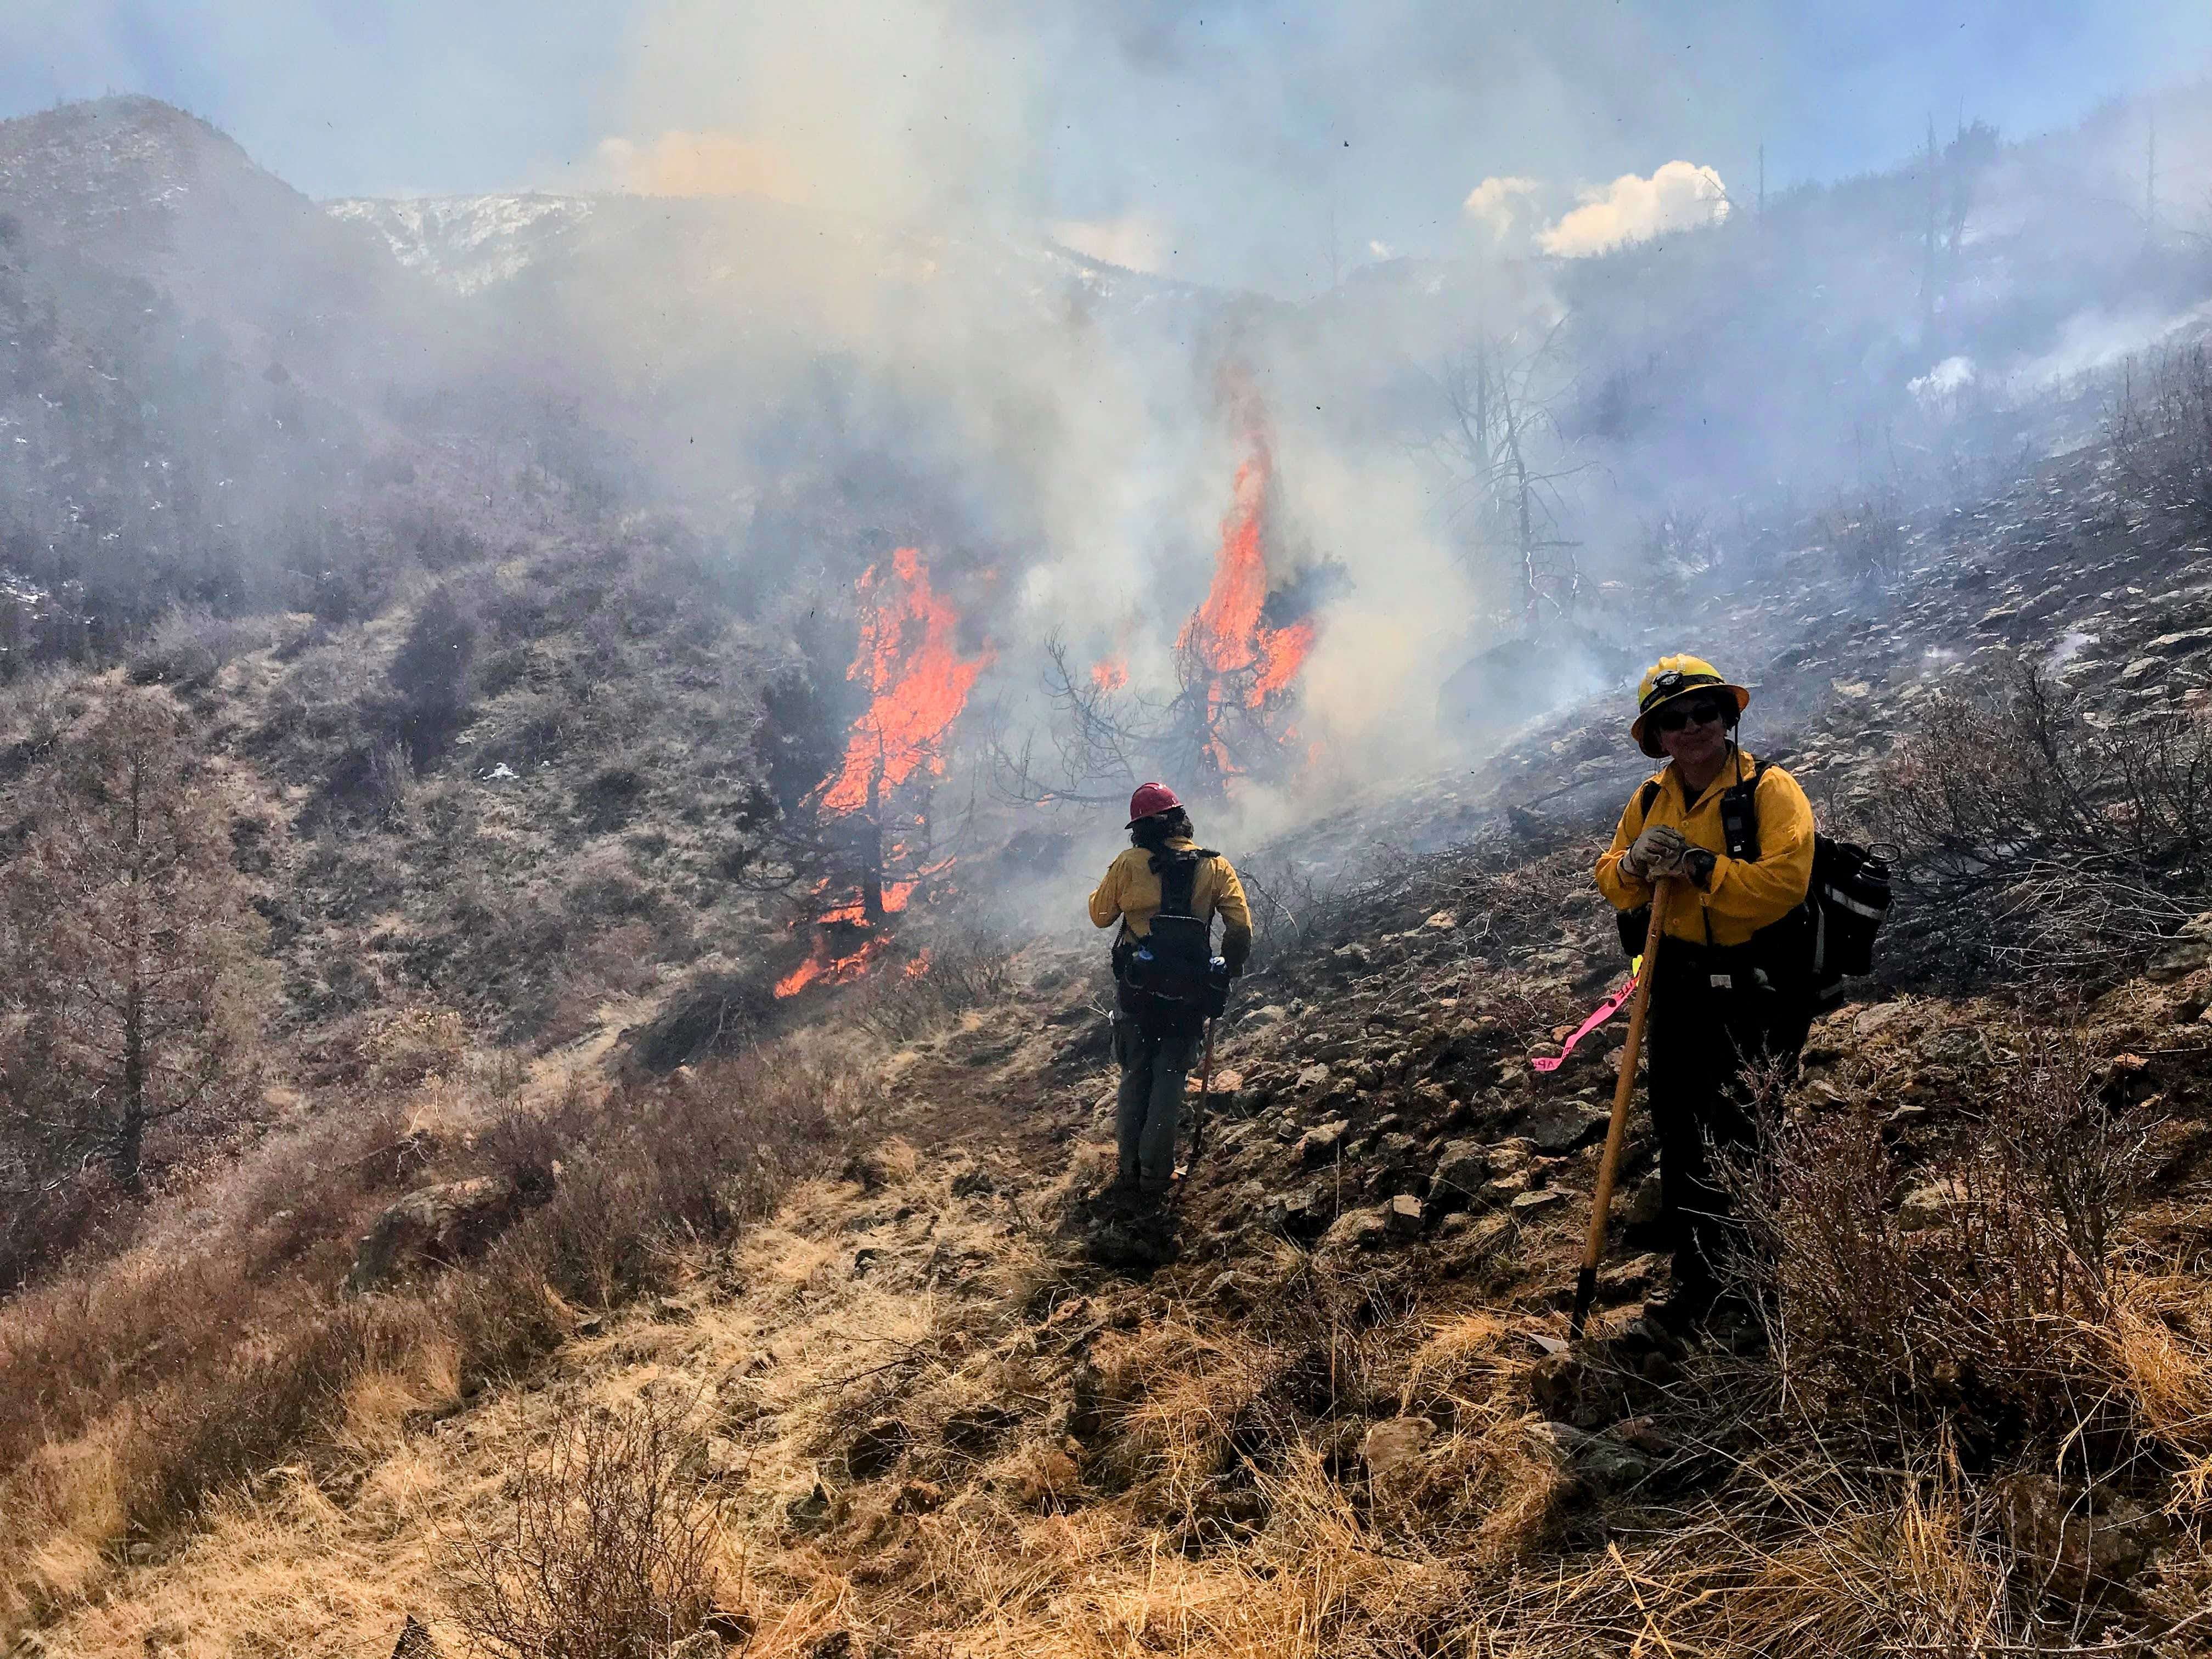
\includegraphics{../Images/SPF} \caption[Stove Prairie Fire]{Watching a juniper tree torch on the Stove Prairie Fire in April 2023. Photo by author.}\label{fig:figureTitle14}
\end{figure}

In rural, unincorporated communities around the state of Colorado, local, volunteer fire districts are the first line of defense against wildfires as well as other hazards. Perhaps because of the aforementioned widespread community involvement with the PCFPD, most community members understand the multiple risks associated with living and recreating up the Poudre, from rockfall on the narrow canyon highway to trees falling on cars at a national forest campground. Rather than bucking responsibility related to living in the WUI, people up the Poudre have nuanced understandings of the complex ecosystem of risks involved in living there, of which residing in a fire adapted landscape is but one consideration. Furthermore, PCFPD volunteers, and the wider community of earlier volunteers, are assets to a wide range of stakeholders and land managers because of their presence and service in a landscape where the jurisdiction of responding to emergencies or wildfires would otherwise fall entirely to the county or to the USFS, whose employees live in Fort Collins, up to three hours away from the areas to which PCFPD responds.

\begin{figure}
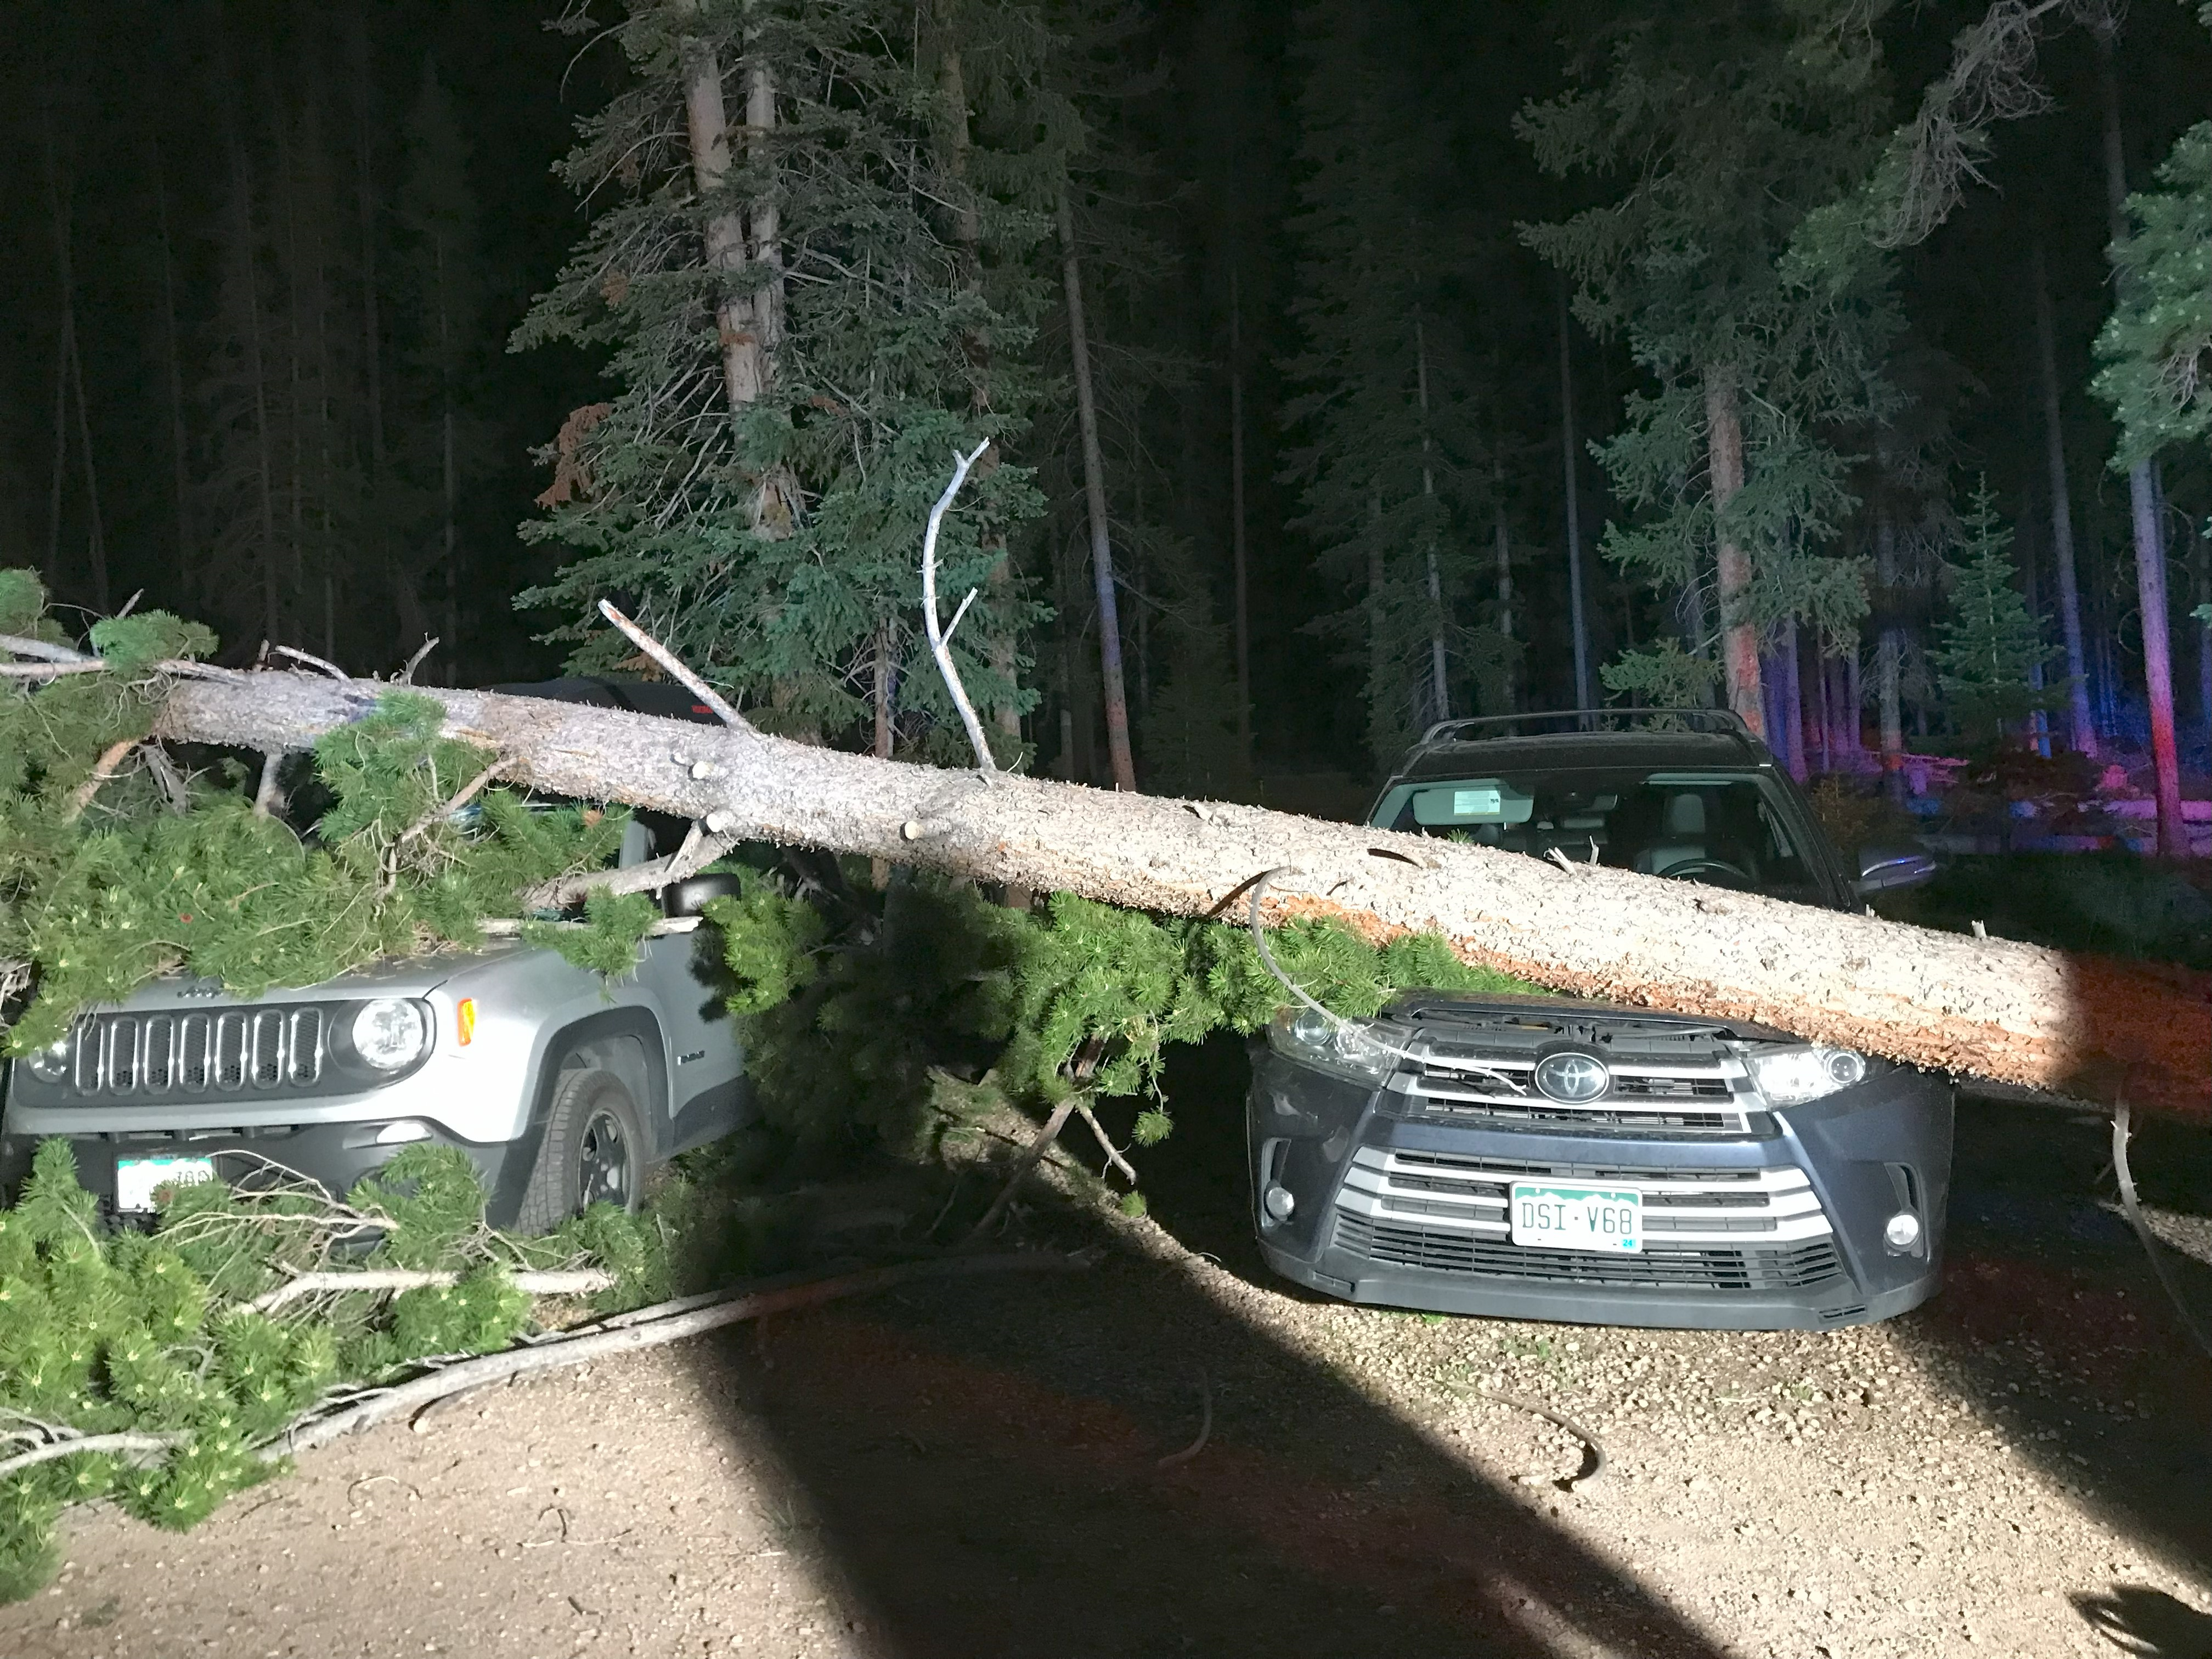
\includegraphics{../Images/PCFPD} \caption[Trees over cars]{Trees fallen over cars at a U.S. Forest Service campground after heavy rains. Photo by author.}\label{fig:figureTitle15}
\end{figure}

\subsubsection{\texorpdfstring{\emph{There's going to come a day when Colorado's going to catch on fire}}{There's going to come a day when Colorado's going to catch on fire}}\label{theres-going-to-come-a-day-when-colorados-going-to-catch-on-fire}

Back before 2012, the Arapaho-Roosevelt National Forest was known as the ``asbestos forest'' to wildland firefighters based out of Fort Collins because it never seemed to burn. People in the Poudre spoke about small wildfires they had previously experienced which were quickly put out, and there is a record of wildfires in the general area dating from 1893 (\citeproc{ref-fryCachePoudreRiver1954}{Fry 1954}; \citeproc{ref-schneiderForestFiresPoudre2020}{Schneider 2020}). The 2012 High Park Fire was the first wildfire with devastating consequences for the Poudre Canyon, including evacuations, loss of homes, and subsequent flooding. Most of these impacts were felt by lower canyon residents because the wildfire never entered the upper portion of the canyon, although it affected access and shaped expectations throughout the Poudre Canyon about the future possibility of destructive fire.

At the time, the PCFPD fire chief lived in the lower Poudre. He and his wife had moved to the Poudre in 2008 from California, where he had been a career structural and wildland firefighter. The High Park Fire began on June 8, 2012 and was contained by July 1, 2012, before the onset of the summer monsoon in Colorado, characterized by frequent afternoon thunderstorms usually beginning in July and lasting into August (\citeproc{ref-NorthAmericanMonsoon2023}{{``North {American Monsoon}''} 2023}). Based on his wide-ranging experiences with wildfire in California, Chris, the fire chief, expected that flooding from tributaries that burned would occur during the summer. He asked the Larimer County Office of Emergency Management for sandbags in anticipation but was told ``It doesn't flood here. This is a different kind of soil than in California.''

As Chris predicted, when the monsoon began, the tributaries began flooding and damaging homes, and the county did eventually provide sand and bags to be filled. Later they even provided an automated sandbag filler, which Chris would fill with sand using his tractor. At first, it was up to the community to fill the bags, and Chris again used his prior experience to help properly fill bags and place them to deflect water effectively. Even those in the community who did not need sandbags jumped in to help. ``I mean, it just doesn't happen like that in L.A.,'' Chris explained.

These experiences during the High Park Fire point to the learning curve that comes with living with fire, by government agencies and the public alike. In 2013, heavy rains resulted in a swollen Poudre River which primarily impacted Fort Collins with extensive flooding, through which lower reaches of the Poudre River flow. The 2013 floods jumpstarted a number of watershed coalitions --- including CPRW --- along the Front Range through funding provided by a Community Development Block Grant for disaster recovery through Housing and Urban Development (HUD). These back-to-back disasters in 2012 and 2013 shaped how individuals and various government agencies perceive wildfire and flooding and respond to it today. For many in the upper Poudre, PCFPD firefighters notwithstanding, the kind of extreme fire behavior, high burn severity, and massive acreage that characterized the CPF eight years after High Park and which dramatically altered the landscape in which they live was not something they had intimately experienced before. The 2012 High Park Fire was the first major wildfire to dramatically impact the canyon, but even it did not burn for as long, affect as much acreage, or burn at such high levels of severity (\citeproc{ref-HighParkFire2012}{{``High {Park Fire}''} 2012}). I heard from multiple community members in the upper Poudre that they always associated flooding risk with the main stem of the Poudre River, not with its tributaries. This was informed by either knowledge of an 1891 dam breach which caused a catastrophic flood on the Poudre or of the Big Thompson Flood of 1976 in a neighboring canyon which killed 144 people. People in the upper Poudre had rare experiences with flooding on tributaries. Black Hollow Creek, which turned into the tragic debris flow in 2021, was mostly a babbling brook over the course of sixty years during which one of the Black Hollow residents had observed it. The debris flow changed the way people understand the relationship between fire and flood and the potential for much smaller watersheds to present the greatest danger of flooding.

At the 2023 Colorado Wildland Fire Conference, some fire and watershed practitioners and scientists expressed incredulity that landowners who were informed the tributaries near their homes were likely to flood after the CPF did not believe it because they and their ``father's grandfather'' (to quote one of the scientists) had never experienced anything like it. However, I argue that it is reasonable to understand the capacity of a creek to behave in a certain way based on empirical observations collected over a lifetime and historical, situated knowledge passed down from one generation to the next. People who have experienced wildfire and who may be exposed to subsequent hazards like flooding need time and empathy to adjust to the rapidly changed realities of living in a post-wildfire landscape. Part of living with fire is living with altered environments, with cascading hazards, and in some cases, devastation.

Messaging directed toward those who live in fire adapted landscapes implies that people residing in these areas need to learn to live with fire. Yet the Poudre Canyon and its residents have been living with fire for a long time, recounted by multiple longtime residents. Volunteers with the PCFPD respond to a number of wildfires each year. It seems that what is actually meant is that people need to learn to live with catastrophic fire, as well as potentially destructive post-fire flooding. Policymakers and practitioners communicating with communities exposed to wildfire risk need to acknowledge existing relationships with fire and be explicit about what being a fire adapted community means in the context of extreme fires. I suggest that living with fire is not just about removing vegetation from around one's home. It's a process of recalibration in response to rapid, large scale, and ongoing changes to vegetation and hydrology (\citeproc{ref-daurioTemporalRecalibrationsLearning2023}{Daurio 2023}). Living with fire is also about learning how to navigate complex bureaucratic and administrative systems during and after the fire and coping with loss. This loss may include loss of life, loss of a home, loss of control, or loss of sense of place.

Some of these impacts are not limited to those who live within the burn area. Just as wildfire smoke and water quality affect people far beyond the perimeter of the wildfire, so do the emotional and social dimensions of loss and change. The Fort Collins-based researchers and practitioners I interviewed experienced CPF on a deeper, more personal level because it was in their backyard, in their watershed, at their research sites, and in the places they like to recreate. As one person involved in wildfire policy and forest management for decades said about his colleagues, ``People were really kind of wrecked in a lot of different ways. \ldots this is our watershed. This is a place where people have family histories, even people that moved here recently. The first thing they did was to go up and camp, hike, whatever they do. So, people have very strong personal place connections, sense of place for this whole area.'' Living with fire is a process, not an event, or a list of mitigation tasks to check off. And we are all of us --- those who live in fire adapted landscapes, those who study fire adapted landscapes, and those who govern and manage them --- engaged in a process of recalibration, often in response to a wildfire that impacts us personally.

\subsection{Discussion}\label{discussion-1}

This ethnographic case study reflects the circumstances of one community affected by wildfire and post-fire flooding and therefore embodies one set of options for how stewardship with private landowners can be cultivated. Other communities facing or already having experienced wildfire will have different perspectives and geographies. This research contributes to literature emergent from CPF and recent wildfires and offers a valuable perspective on how a rural community facilitates stewardship of both private and federal lands and the water that runs through them, and helps mitigate hazards to the benefit of populations outside the community. In addition to the examples I have provided from the Poudre, I advocate for more cross-jurisdictional partnerships with rural communities toward a shared goal of learning how to better live with fire. I argue that reconceptualizing communities residing in fire adapted landscapes as potential stewards opens up pathways for mobilizing these partnerships. It also centers agency for living with fire with communities. Below are several examples of what centering agency could look like.

A study on voluntary and regulatory wildfire risk reduction in two rural unincorporated communities in Wyoming and Utah showed a preference in these communities for greater local agency in implementing and managing wildfire mitigation (\citeproc{ref-edgeleySupportRegulatoryVoluntary2020}{Catrin M. Edgeley, Paveglio, and Williams 2020}). There are good examples of this already happening. In California and a number of other states, for example, Prescribed Burn Associations (PBAs) are community-based, mutual-aid networks which support private landowners in burning on their own lands (\citeproc{ref-CaliforniaPrescribedBurn}{{``California {Prescribed Burn Associations Cal PBA}''} 2024}). Organizations like the Fire Networks, The Ember Alliance, and Fire Adapted Colorado advocate for expanding agency over fire management to include local capacity (\citeproc{ref-zotero-10034}{{``About''} 2024}; \citeproc{ref-EmberAllianceChanging}{{``The {Ember Alliance} -- {Changing Lives}, {Restoring Landscapes}''} 2022}; \citeproc{ref-FireAdaptedColorado}{{``Fire {Adapted Colorado}''} 2022}). A recent Fire Networks blog post suggested harnessing the ranching concept of ``neighboring'' for community wildfire mitigation initiatives (\citeproc{ref-burchfieldNeighboringAntidoteSeparation2024}{Burchfield 2024}). There is also emergent research examining the idea of community-based forestry on land owned by different landownership entities and suggestions for further research that examines opportunities for community-based wildfire risk management (\citeproc{ref-davisCommunitybasedForestryFederal2020}{E. J. Davis et al. 2020}). Stewardship of lands which is co-created by multiple government and nonprofit actors reflects already existing federal goals for addressing wildfire governance (\citeproc{ref-FIREReportWildland2023}{{``{ON FIRE}: {The Report} of the {Wildland Fire Mitigation} and {Management Commission}''} 2023}). Building on previous work, I encourage the added inclusion of private landowners in consideration of these objectives and in post-fire watershed management (\citeproc{ref-charnleyFosteringCollectiveAction2020}{Charnley, Kelly, and Fischer 2020}; \citeproc{ref-kirklandTakingAlllandsApproach2021}{Kirkland and Charnley 2021}).

There is a concerted push on the part of county, state, and federal agencies to create fire adapted communities in order to contend with increasing wildfire exposure to properties and lives. Part of this advocacy is encompassed within messaging crafted by fire and emergency managers to reach those who live in the WUI. In this paper, I question the usefulness of using the term WUI because it homogenizes people, places, and local contexts of wildfire risk. It also geographically limits our perception of wildfire risk and separates how we think about and prepare for other wildfire-related hazards such as smoke and post-fire flooding, the impacts from which are felt far beyond the burn perimeter.

I advocate moving away from the narrative of personal responsibility as a strategy to encourage homeowners to undertake wildfire risk reduction efforts, as it is simply not supported by the literature or data on risk perception and homeowner action/inaction. This narrative also assigns liability to individual homeowners who live in the WUI and creates a false notion that only those who live in the WUI are subject to wildfire-related risks. In cultivating fire adapted communities, I think it is more helpful to characterize wildfire as something with which everyone in society has to contend, whether it is through direct contact with wildfires, wildfire smoke, or post-fire hazards such as flooding or compromised water quality. I argue that reshaping the narrative about those who live in fire adapted landscapes encourages a shift in perspective to understand the people in these communities as allies in cultivating the practice of living with fire. Centering co-stewardship opens up possibilities for collaboration and collective action that may otherwise be foreclosed. Approaching frontline communities as custodians allows us to center care for their well-being and that of the surrounding environment.

\subsection{References}\label{references-2}

\clearpage

\section{Accepting Ecologies of Impermanence: Sensemaking in the Aftermath of the Cameron Peak Fire}\label{accepting-ecologies-of-impermanence-sensemaking-in-the-aftermath-of-the-cameron-peak-fire}

\renewcommand{\thefigure}{4.\arabic{figure}}
\setcounter{figure}{0}
\renewcommand{\thetable}{4.\arabic{table}}
\setcounter{table}{0}
\renewcommand{\theequation}{4.\arabic{equation}}
\setcounter{equation}{0}

\subsection{\texorpdfstring{Introduction: \emph{A Convergence of All These Convergences}}{Introduction: A Convergence of All These Convergences}}\label{introduction-a-convergence-of-all-these-convergences}

In \emph{Young Men and Fire}, Norman Maclean, the author of \emph{A River Runs Through It}, weaves a historical narrative around the circumstances leading to the death of thirteen smokejumpers on the 1949 Mann Gulch Fire in Montana. Maclean tries to make sense of the ``individual components'' (289) of terrain, wind, fire, and men that form the basis of this tragedy but lands on a story of a `convergence of all these convergences' (288) that results in a ``conflagration'' (289), a moment ``seemingly beyond the laws of nature, blown into a world where human values and seemingly natural laws no longer apply'' (289).

When the 2020 Cameron Peak Fire (CPF) engulfed my family's historic home which had been passed down through five generations over 127 years, in what a fire behavior analyst described as ``a wall of fire,'' (personal communication, 9/17/20), I set out to make sense of the convergences which made something like the CPF possible. The CPF was an extreme wildfire, starting in mid-August and burning for 112 days into the heart of winter in Colorado. While it became and remains the state's largest wildfire, it was hardly the only wildfire that year in Colorado to defy expectations. In a world where wildfires are becoming larger (\citeproc{ref-rodmanHistoric2020Fire2022}{Kyle C. Rodman et al. 2022}), of higher severity (\citeproc{ref-wassermanClimateInfluencesFuture2023}{Wasserman and Mueller 2023}), spreading more rapidly (\citeproc{ref-balchFastestgrowingMostDestructive2024}{Balch et al. 2024}), and lasting longer (\citeproc{ref-balikBiogeographicPatternsDaily2024}{Balik et al. 2024}), this paper examines how those who lived through CPF, those who study it, and those who fight and manage wildfire engage in sensemaking to understand wildfire, post-fire impacts, and uncertainty in the context of such landscapes. Sensemaking practices following disaster can (re)shape relations with the material world in a way that broadens temporal and conceptual horizons associated with ecological and climatic uncertainty and degradation, with important policy implications. Engaging ethnographic research methods, I immersed myself in the landscape in which the wildfire had occurred, living in the Poudre Canyon in northern Colorado and interviewing a diverse cohort of people representing community members, fire practitioners, and scientists, to understand wildfire through the lens of their experiences and knowledge systems.

In response to experiences of extreme wildfire and the cascading hazards which unfold as a result, I suggest that individuals, communities, and governments undergo a process of recalibration in ways of knowing the environment. Here I define recalibration ``as a process by which, through cataclysmic moments of change, we come to understand the contingent histories and futures'' (\citeproc{ref-daurioTemporalRecalibrationsLearning2023}{Daurio 2023}) of our human lives as entangled with other than human material formations and temporal frames. Disaster in the form of wildfire can render past processes of landscape change knowable and recognizable in the present and reorient future expectations in relation to uncertain climates, weathers, and environments. For participants, cumulative experiences and study of wildfire over time embeds ways of knowing in the context of previous methods of recalibration. Participants across all three interview groups engage in similar kinds of processual sensemaking regarding loss, transformation of the landscape, and future uncertainty, manifesting in an acceptance of what I call ecologies of impermanence. The geographer Caitlin DeSilvey, grappling with the impermanence of a disappearing coastal path in Cornwall in the U.K., similarly refers to ``developing alternative ways of approaching foundered things, and allowing them to carry on with their changes with their ambiguous energies intact'' (\citeproc{ref-desilveyFounderedOtherObjects2020}{DeSilvey 2020}: 226). Research participants, as part of making sense of material reconfigurations through fire and flood, largely attribute the destruction of lives, property, and landscapes to the forces of nature. I argue that this perception of nature as agentive enable participants to grapple with different kinds of loss --- physical, affective, and environmental, among them --- by normalizing loss within an ecological understanding of wildfire and post-fire flooding. This is the case even though the CPF was the most extreme wildfire the majority of participants had ever experienced. Across the three groups, participants express acceptance of our inability to control wildfire. For scientists and some practitioners, lack of control is not equated with lack of agency. Agency is expressed as an articulation of values defining a vision of ecological priorities. More specifically, extreme wildfires and climate change may be transforming forested landscapes in the western U.S., but we can choose where to implement actions toward a particular ecological vision based on what we value in those landscapes. Recalibration is born out of cumulative sensemaking, indicating that people can cope with significant personal and environmental changes wrought by wildfire by engaging in processes of sensemaking over time, sensemaking which is shaped by acknowledging that matter is agential and constitutes the ``ongoing reconfigurings of the world'' (\citeproc{ref-baradMeetingUniverseHalfway2006}{Barad 2006}: 141).

This paper explores how people make sense of a particular kind of wildfire. I conceptualize wildfire as a convergence of the multiple materialities, temporalities, and agencies of ecologies, terrain, weather, climate, and human actors, the confluence of which makes every wildfire unique. Wildfire can have both constructive and destructive properties (Fowler 2021), and landscapes across the American West are fire-adapted, meaning that wildfire is an ecological necessity (Lotan 1976; Fitzgerald 2005; Prichard et al.~2021). In the case of the CPF, the convergence of factors resulted not just in a wildfire, but in a ``conflagration'' (\citeproc{ref-macleanYoungMenFire1992}{Maclean 1992}: 289), a term I use to signify a wildfire exhibiting extreme characteristics --- high rate of spread, high burn severity, and unpredictable behavior --- which is beyond human capacity to control, that is also a disaster, meaning one which has negative social-ecological impacts affecting people's lives. I build on but diverge from the definition of extreme wildfire events (\citeproc{ref-tedimDefiningExtremeWildfire2018}{Tedim et al. 2018}), based on fire behavior, unpredictability, and lack of capacity to control, and from megafires (\citeproc{ref-kodasMegafireRaceExtinguish2017}{Kodas 2017}; \citeproc{ref-swainEraMegafiresCrisis2018}{Swain, Kolden, and Abatzoglou 2018}), typically characterized by scale, intensity, and devastation, to focus on the lived experiences of people in a particular landscape context. In using the term conflagration, inspired by Maclean's multidecadal meaning-making of the Mann Gulch Fire, I am interested in capturing the idea and experience of a wildfire existing outside normative expectations alongside its complex consequences for people's lives. I employ the concept of \emph{overtime} to theorize how conflagrations represent a social-ecological system that is over capacity, operating in climatic overtime, that is, outside the historic range of variability.

In what follows below, I contextualize the CPF and the 2020 fire year within the literature on extreme wildfires and review anthropological engagements with landscape, temporality, and materiality to frame how people understand their own lives and experiences within the different timescales and lifecycles of human and other than human ecologies in the formation of disaster. I explore previous scholarship on sensemaking in wildfire, disaster, and heritage contexts. I describe my landscape-based methodology and, drawing on sustained ethnographic engagement with the upper Poudre Canyon community in northern Colorado, I offer empirical examples of how community members, practitioners, and scientists are making sense of the CPF, the flooding and debris flows which came after it, and how they relate to a transformed landscape subject to the material consequences (\citeproc{ref-kosekUnderstoriesPoliticalLife2006}{Kosek 2006}) of fire and flood.

\subsection{The Poudre Canyon, the Cameron Peak Fire, and the 2020 Fire year}\label{the-poudre-canyon-the-cameron-peak-fire-and-the-2020-fire-year}

The Poudre Canyon is made up of several unincorporated communities (\citeproc{ref-LarimerCountyColorado2024}{{``Larimer {County}, {Colorado}''} 2024}), meaning that Larimer County, and its Board of County Commissioners with three elected officials, is the defacto governing body. The Poudre Canyon Fire Protection District (PCFPD) is a local government entity whose jurisdiction for emergency response and wildfire management encompasses the entire populated length of the Poudre Canyon (\citeproc{ref-Us2024}{{``About {Us}''} 2024}). The river corridor itself is made up of 85\% federal lands, with only 2,000 out of 25,000 acres in private ownership (\citeproc{ref-CachePoudreWild1990}{{``Cache {La Poudre Wild} and {Scenic River Final Management Plan}''} 1990}) and is where most of the houses of 750 full-time and 1,500 part-time residents are distributed (\citeproc{ref-Us2024}{{``About {Us}''} 2024}). The lands beyond the corridor are primarily owned by the US Forest Service (USFS). Private lands are mostly situated along the river where flatter ground makes it easier to build, although in the lower Poudre a few, comparatively newer, houses have been built on ridgelines. Alluvial fans formed many of these flatter areas, and in other cases they are part of the river's old floodplain, illustrating the dynamic fluvial properties of the Poudre in its geomorphological formations. In populated areas of the Poudre, some of the river's thousands of miles of tributaries pass through private lands in their lowest reaches before reaching the river. The largest population clusters in the Poudre today reflect historic colonial settlement patterns, built in proximity to a creek and on land where they could ranch or mine. This topography, formed by thousands of years of geologic movement, combined with land use and ownership established over shorter timescales, help shape how people in the Poudre experience wildfire and post-fire flooding.

The CPF began on August 13, 2020, in a high elevation, subalpine forested area at the top of the canyon during a year of significant drought characterized by hot, dry weather, low snowpack, and early runoff, among other variables (\citeproc{ref-bolingerClimateChangeColorado2024}{Bolinger et al. 2024}). These subalpine forests experienced significant tree mortality stemming from a series of large bark-beetle outbreaks 15-25 years ago (\citeproc{ref-rodmanEffectsBarkBeetle2021}{Kyle C. Rodman et al. 2021}). The Poudre River flows through the canyon for forty miles, dropping thousands of feet in elevation as it makes its way toward the plains and supplies water for the hundreds of thousands of people in the populous Front Range cities of Fort Collins and Greeley. Prior to the High Park Fire (HPF) in 2012 and the CPF in 2020, the entire length of the Poudre was heavily forested, with diverse forest types following elevational gradients.

In discussing why the CPF and other fires in 2020 can be characterized as particularly extreme, it is worth noting that there is an ongoing history of small fires in the Poudre Canyon based on a combination of what participants told me, my own memories over the course of my life, and my experiences as a volunteer with the PCFPD. There is also a record of wildfires in the general area dating from 1893 (\citeproc{ref-schneiderForestFiresPoudre2020}{Schneider 2020}), a year in which a large, destructive, out of control fire occurred (\citeproc{ref-fryCachePoudreRiver1954}{Fry 1954}). One of the interview participants recalled the same person who recounted the 1893 wildfire as saying we were due for another one sometime in the 1940s or 1950s, indicating an expectation at that time that recurring wildfire is inherently part of this landscape. The first wildfire in the area in people's memories today that could be characterized as a conflagration occurred in 2012 in the lower Poudre and several nearby communities, destroying 259 homes (\citeproc{ref-HighParkFire2012}{{``High {Park Fire}''} 2012}) and causing significant flooding in nearby tributaries. Based on an interview with a PCFPD firefighter who lived in the lower Poudre at the time, the post-fire flooding took community members and Larimer County by surprise, marking the first time residents and emergency managers in this part of Colorado became familiar with the cascading hazards of fire and post-fire flooding.

It was another eight years before the Poudre Canyon experienced a significant wildfire, and it occurred in a historic year for wildfires across the American West and Pacific Northwest in 2020 (\citeproc{ref-robbinsOregonClimateChange2021}{W. G. Robbins 2021}; \citeproc{ref-keeleyLargeCaliforniaWildfires2021}{Keeley and Syphard 2021}). It is also worth noting that the 2020 wildfires occurred during the COVID-19 pandemic, complicating the logistics associated with firefighting and evacuations, and exacerbating the dangers of exposure to wildfire smoke. The wildfires in 2020 in Colorado reflect uncharacteristic, extreme, and surprising behavior in several ways. First, the state's three largest wildfires, including the CPF, all occurred in 2020, surpassing the previous record set in 2002 by the Hayman Fire at 137,760 acres (\citeproc{ref-ListColoradoWildfires2024}{{``List of {Colorado} Wildfires''} 2024}). Second, prior to 2002, Colorado had never had a wildfire that exceeded 100,000 acres. It was eighteen years before this occurred again, in 2020, a year in which three wildfires grew to over 100,000 acres. The CPF eventually burned over 208,000 acres. Third, the sheer size of the CPF --- and other fires in 2020 --- is attributable to the extreme fire spread which occurred on single day events, a phenomenon increasingly driving cumulative area burned on wildfires in the western U.S. (\citeproc{ref-coopExtremeFireSpread2022}{Coop et al. 2022}). The CPF grew by more than 40,000 acres on Labor Day 2020 in its first major period of growth and nearly reached Fort Collins in the plains in another period of extreme fire spread in mid-October (\citeproc{ref-CameronPeakFire2020e}{{``Cameron {Peak Fire} Is Now One of the Largest Wildfires in {Colorado} History, at {96K}+ Acres''} 2020}). These extreme fire spread events were facilitated by strong winds combined with dry fuels. Wind-driven extreme fire behavior was a characteristic of many wildfires across the West and Pacific Northwest in 2020, which, in combination with high temperatures and fuel aridity, suggest a tripartite convergence of factors influencing high severity, destructive conflagrations (\citeproc{ref-eversExtremeWindsAlter2022}{Evers et al. 2022}; \citeproc{ref-abatzoglouCompoundExtremesDrive2021}{Abatzoglou et al. 2021}) and accounting for a significant percentage of area burned (\citeproc{ref-coopExtremeFireSpread2022}{Coop et al. 2022}).

Fourth, the months during which the CPF occurred and the length of time over which it burned suggest a divergence from historical fire patterns. Typically wildfires 10,000 acres or more have occurred in June or July in Colorado (\citeproc{ref-borsumCameronPeakFire2021}{{``Cameron {Peak Fire}, {Northern Colorado}''} 2021}). Even the destructive 2002 Hayman and 2012 High Park fires began in June and were contained in less than a month (\citeproc{ref-ListColoradoWildfires2024}{{``List of {Colorado} Wildfires''} 2024}). In contrast, in 2020, the CPF began in August, and two other major fires began in September and October, respectively. It is not atypical to experience snow at higher elevations in Colorado in September and October, highlighting how unusual it was for wildfires to exhibit their most destructive behavior during these months and to ignite well outside the typical summer months. The aforementioned strong wind events facilitated this divergent temporal behavior during the autumn months, predicted to occur more frequently due to climate change, particularly in California (\citeproc{ref-gossClimateChangeIncreasing2020}{Goss et al. 2020}). Downslope wind-driven wildfires in the western U.S., frequently associated with spring and fall, rather than summer, have accounted for a large percentage of some of the most destructive fires between 1999 and 2020 and appear to be increasing in frequency (\citeproc{ref-abatzoglouDownslopeWindDriven2023}{\textbf{abatzoglouDownslopeWindDriven2023?}}). The Marshall Fire, Colorado's most destructive wildfire, was a downslope wind-driven fire which occurred on December 30, 2021 and burned 1,000 homes in a day in suburban areas of Colorado's eastern Front Range (\citeproc{ref-doughertyMarshallFireInvestigative2023}{Dougherty and Johnson 2023}). The CPF burned well into Colorado's winter season and lasted for 112 days from August to December 2020, well outside the historical seasonality of wildfires in Colorado (\citeproc{ref-borsumCameronPeakFire2021}{{``Cameron {Peak Fire}, {Northern Colorado}''} 2021}).

The unusual behavior of the 2020 Colorado wildfires, particularly their persistence through the autumn and beginning of winter, resulted in significant disruptions to people's lives. During the CPF, people in the upper most residential area of the Poudre Canyon were evacuated for 73 of the 112 days the fire lasted. While people were under evacuation, the power was shut off by the electric authority to prevent the fire from interacting with live power lines. People who were evacuated quickly, who were not provided the opportunity to return to their homes, or who were unaware the power would be shut off returned home to destroyed refrigerators, and in some cases, damaged floors or break-ins from bears after food rotted and melted out of refrigerators. The CPF destroyed 492 structures across sixteen communities (\citeproc{ref-coalitionforthepoudreriverwatershedCameronPeakFire}{Coalition for the Poudre River Watershed 2023}). Extreme fire spread days overwhelm firefighting resources and can leave communities unprepared to evacuate in time, as happened during a concurrent fire called the East Troublesome (ETF) in October in Colorado. One of my interview participants evacuated to a hotel due to the CPF --- because of COVID-19, hotels were used instead of evacuation centers --- described the parking lot filled with so many evacuees from the ETF, some with nothing but the clothes they were wearing, that it was impossible to walk from the parking lot to the hotel.

The 2020 Colorado and western U.S. wildfires represent a series of conflagrations which overwhelmed the senses and capacities for those experiencing and managing the CPF to predict and respond to extreme, rapidly changing, and hazardous conditions. Subsequent fire years in other locales in the U.S. and Canada indicate similarly overwhelmed fire management capacities, such as the aforementioned 2021 Marshall Fire, the 2023 fire in Lahaina, Maui which killed 102 people and destroyed over 2,200 structures, and the record-breaking Canadian wildfires in 2023 which spanned multiple provinces, evacuated the entire town of Yellowknife in the Northwestern Territories, and caused hazardous levels of wildfire smoke to linger in New York City for days. Emerging from participant narratives of sensemaking in the aftermath of the CPF, I build on Adriana Petryna's idea of ``ethnographic concept work'' to imagine how communities contending with disaster-driven loss and climatic uncertainty might better navigate changing materialities and conditions of \emph{overtime}. Petryna refers to ``runaway change'' in the context of wildfires and climate change writ large, representing the gap between expectations and reality, where change occurs outside the scope of projected models and predictive capacity (\citeproc{ref-petrynaWildfiresEdgesScience2018}{Petryna 2018}).

Although until now, I have focused primarily on conflagrations themselves as the basis for sensemaking, interviews with research participants and my experiences as a participant observer residing in a post-fire landscape reveal that wildfire and watershed hazards and the environmental changes wrought by both are inextricably linked, both ecologically (\citeproc{ref-wilsonConnectivityPostfireRunoff2021}{Wilson et al. 2021}) and experientially. I advocate for conceptually connecting fire and post-fire affective and material dimensions as an acknowledgement of fire as a phenomenon which sets in motion a series of social and ecological processes with long term implications. For those community members I interviewed, experiences of post-fire repercussions are delineated from those which occurred during the fire, but the fire is characterized as the origin point, without which nothing else that followed would have occurred. I use the language of fire and post-fire to distinguish these two periods from each other in order to address the ways an active wildfire functionally impacts people's lives differently than the post-fire period. The latter period is conditioned by fire and characterized by more nebulous time horizons and distinct government response mechanisms. The reality of connected, unfolding consequences stemming from the CPF resists the idea of episodic timeframes (\citeproc{ref-shneidermanFramingIssuesPolitics2014}{Shneiderman and Snellinger 2014}) representing fire and post-fire periods at the same time that it is important to draw meaningful distinctions between the two to reflect the experientially different states of emergency and protraction. The ongoing landscape changes initiated by extreme wildfires --- particularly in mountainous watersheds like the Poudre Canyon --- and the impacts these changes have for people's lives, persists for years after the wildfire. Just as the presence of wildfires in the western U.S. indicate that we live in fire-prone landscapes, post-fire hydrological changes reveal past and potential processes of sedimentation, erosion, and deposition (\citeproc{ref-robichaudQuantifyingLongtermPostfire2020}{Robichaud et al. 2020}; \citeproc{ref-sosa-perezWildfireEffectsRoad2017}{Sosa-Pérez and MacDonald 2017}). Thus, making sense of conflagrations cannot be disentangled from recalibrating our understanding of landscape change also based on post-fire disturbances. By way of example, for the first three summers after the CPF, flooding and debris flows in the Poudre Canyon caused damage to roads, bridges, and homes, sometimes blocking access to property. Tragically, a debris flow in Black Hollow Creek in July 2021 killed four people and destroyed six homes. In the Poudre Canyon, some people were impacted more by either the wildfire or post-fire flooding, and some were significantly impacted by both. People's contingent experiences of fire and flood are reflected in their processes of sensemaking.

\subsection{Theorizing Landscape}\label{theorizing-landscape}

\subsubsection{The Material Traces of Landscapes}\label{the-material-traces-of-landscapes}

This research addresses how lived experiences of disaster impact how people relate to the social, political, historical, and environmental landscapes in which they live and work. Building on earlier scholarship in anthropology and geography theorizing landscape, I understand landscapes as ``spatial and temporal fields\ldots co-constituted by the structure and dynamics of environments and by human action'' (\citeproc{ref-morrisonPuttingTimeIts2016}{Kathleen D. Morrison 2016}: 621). Landscape is a useful theoretical concept for understanding wildfire because it represents the underlying processes of inhabitance and the relations with the plant and animal species and climatic systems encountered within, through, and on it (\citeproc{ref-braceHumanGeographiesClimate2010}{Brace and Geoghegan 2010}: 289). A wildfire fundamentally alters these relations and renders visible the ``material legacies'' (\citeproc{ref-tsingWhenThingsWe2019}{A. Tsing 2019}: 230) of particular landscapes, both through fire itself and through processes initiated by the wildfire (\citeproc{ref-wohlBiogeomorphicInfluencesRiver2022}{Wohl et al. 2022}), such as flooding.

The theory of punctuated equilibria was developed in 1972 to describe biological evolution in geological time (\citeproc{ref-elredgePunctuatedEquilibriaAlternative1972}{Elredge and Gould 1972}). The theory explains that species tend to originate in punctuated geological moments and then remain stable for much of their evolutionary existence (\citeproc{ref-gouldPrimaryClaimsPunctuated2009}{Gould 2009}). Since then, the theory has been applied to human biocultural evolution (\citeproc{ref-obrienPunctuatedEquilibrium50}{\textbf{obrienPunctuatedEquilibrium50?}}), public policy changes (\citeproc{ref-jonesThereHerePunctuated2012}{Jones and Baumgartner 2012}), and environmental change (\citeproc{ref-wohlRhythmsChangeRocky2016}{Wohl 2016}). Fluvial geomorphologist Ellen Wohl refers to ``punctuated rhythms'' to describe how changes to the landscape tend to occur during episodic periods of rapid shifts, precipitated by, for example, the melting of glaciers (\citeproc{ref-wohlRhythmsChangeRocky2016}{Wohl 2016}). These periods of change occur on different timescales depending on the disturbance. In mountain watersheds, wildfire, which can occur frequently depending on species' fire regimes and fire management, represents one of these punctuations. Wildfire creates a ``disturbance cascade'' (\citeproc{ref-wohlBiogeomorphicInfluencesRiver2022}{Wohl et al. 2022}: 1) resulting in more water and sediment being transported to the river (\citeproc{ref-wellsEffectsFireGeneration1987}{Wells 1987}) and an increased likelihood of debris flows (\citeproc{ref-hochHydrogeomorphicRecoveryTemporal2021}{Hoch et al. 2021}; \citeproc{ref-rengersLandslidesWildfireInitiation2020}{Rengers et al. 2020}).

Wildfires reveal both that landscapes circumscribe particular patterns --- an alluvial fan indicates where sediment deposition may occur again --- and are unfinished (\citeproc{ref-cresswellLandscapeObliterationPractice2003}{Cresswell 2003}) and ``open to emerging forms and possibilities''. The materialisms of landscapes shape and are shaped by the ``lived material practices'' of human beings, manifested as the ``consequential materialisms'' of the histories and politics of nature ``enabling certain understandings and narratives'' (\citeproc{ref-kosekUnderstoriesPoliticalLife2006}{Kosek 2006}: 284) of landscapes and constricting others. Recognizing the sociopolitical and environmental co-constitutiveness of landscapes conceptualizes the material world as both animate and imbued with agency, represented by flows, processes, and substances (\citeproc{ref-ingoldBeingAliveEssays2011}{Ingold 2011}), which is particularly illustrative of its relevance for exploring the Poudre Canyon. It's a landscape shaped by past and continuous movement, from its creation as a glacier- and river-formed valley to its network of tributaries through which nutrients and silt and the traces of old mining operations are mobilized along their way to join the Poudre River, to its history of fire suppression by forest managers and its elevationally-distributed forested, fire-adapted ecosystems.\footnote{The history of intentional burning by Indigenous peoples for various purposes in the Colorado region is much less extensive compared to California. Scholars do not agree on the extent to which anthropogenic burning influenced fire regimes on a landscape or regional scale in Colorado or the Rocky Mountains, but studies suggest that this may have varied widely depending on human settlement pattern and population size, among other factors (\citeproc{ref-bakerIndiansFireRocky2002}{Baker 2002}; \citeproc{ref-pyneInteriorWestFire2018}{Pyne 2018}; \citeproc{ref-allenLotsLightningPlenty2002}{Allen 2002}; \citeproc{ref-grissino-mayerClimaticHumanInfluences2004}{Grissino-Mayer et al. 2004}).} For those whose lives intersected with the CPF, the fire disrupted perceived ecological stability and made the world more visible as ``a dynamic process of intra-activity and materialization'' (\citeproc{ref-baradMeetingUniverseHalfway2006}{Barad 2006, 140}).

\subsubsection{The Temporal Interventions of Wildfire}\label{the-temporal-interventions-of-wildfire}

Wildfires are the result of a convergence of different scalar and temporal ecological (\citeproc{ref-pausasBurningStoryRole2009}{Pausas and Keeley 2009}), meteorological, climatic (\citeproc{ref-higueraRecordsettingClimateEnabled2021}{Higuera and Abatzoglou 2021}) and anthropomorphic processes, interacting with terrain (\citeproc{ref-nealeEternalFlameElemental2019}{Neale, Zahara, and Smith 2019}) that condition the possibility of their existence and shape the nature of their outcomes. Coming to understand how these processes spatially intervene with human timescales in the context of wildfires can help people recalibrate how they relate to the dynamic landscapes they inhabit. On account of climate change, these timescales are rapidly shifting and conditioning different potentials for wildfires to occur and also impacting their length, size, and severity (\citeproc{ref-gossClimateChangeIncreasing2020}{Goss et al. 2020}; \citeproc{ref-diffenbaughVerificationExtremeEvent2020}{Diffenbaugh 2020}; \citeproc{ref-borundaScienceConnectingWildfires2020}{Borunda 2020}). Part of recalibration is not only renegotiating relationships with the material world but also with time. I build on theorizations of temporality to contextualize how experiences of fire expand our sense of time and of our place in time, through the concepts of geological time, \emph{becoming}, and \emph{overtime}.

The paleontologist Stephen Jay Gould wrote about two different kinds of geological time and argued that both are necessary for understanding deep time. Time's arrow underscores the uniqueness of each moment in geological history and the significance of temporal sequencing, whereas ``the metaphor of time's cycle captures those aspects of nature that are either stable or else cycle in simple repeating (or oscillating) series'' (\citeproc{ref-gouldTimesArrowTimes1987}{Gould 1987}: 196). These two representations of geological time are appropriate for understanding wildfire today, and for contextualizing what wildfire can reveal about a geological past that informs material formations in the present. Along a similar vein, Marcia Bjornerud writes about how geological thinking can render timescales beyond the human lifespan more legible, what she refers to as ``timefulness'' (\citeproc{ref-bjornerudTimefulnessHowThinking2018}{Bjornerud 2018}), or an awareness of the earth's temporal rhythms outside our human lives. The CPF enabled people to apprehend time's cycle of wildfire --- and flooding --- as naturally recurring phenomena in the Poudre Canyon. One woman I spoke with discussed the dissonance between relying on knowledge accumulated over 100 years of inhabitance to determine flood risk for her house versus new found geological knowledge realizing that her house was built on an alluvial fan, indicating prior patterns of flooding and the possibility of its recurrence. Time's arrow points to the ``contingent moments of complex historical pathways'' (\citeproc{ref-gouldTimesArrowTimes1987}{Gould 1987}: 196), the convergences of policy, land use, climate, and weather that led to the CPF burning when and where it did. In the post-fire reckoning , participants spoke about contributing factors to the CPF, both those factors occurring on shorter timescales, such as the hot, dry weather that fall, and on longer timescales, such as the density and distribution of beetle-killed trees in the area where it started.

The anthropologist Townsend Middleton, researching declining quinine plantations in India, writes about the particular temporalites emergent from ruins, what he calls the ``becoming-after,''in the unmakings and potential remakings'' (\citeproc{ref-middletonBecomingLivesPoliticsQuinines2021}{Middleton 2021}: 287) of material worlds. Middleton theorizes \emph{becoming} as leaving open possible futures. For those living, working, and researching in the Poudre, experiencing the CPF widened the aperture of both past and future temporalities, and of the material processes which came before and what might become in the future. We tend to assess what is possible in the future by what we have known in the past (\citeproc{ref-desilveyMakingSenseTransience2012}{DeSilvey 2012}), but the past can become more knowable through experiences of punctuated moments in ecological time. In places like the Poudre Canyon, with long histories of inhabitance and strong attachment to place, environmental changes (\citeproc{ref-berroetaPlaceSubjectivityContinuum2021}{Berroeta, de Carvalho, and Castillo-Sepúlveda 2021}; \citeproc{ref-crateSakhaAlaasPlace2021}{\textbf{crateSakhaAlaasPlace2021?}}) or ``shock events'' (\citeproc{ref-schlosbergDisasterPlaceJustice2020}{Schlosberg, Della Bosca, and Craven 2020}: 239) like the CPF create a ``temporal rupture, manifesting as dissonance between past experiences, present realities and future ideas of sociality and sense of self in place'' (\citeproc{ref-asklandLivedExperiencesEnvironmental2018}{Askland and Bunn 2018}: 18).

Although labor capacity in firefighting were not the focus of my research, it is a germane to discussions of systems operating over capacity, or in \emph{overtime}. Wildland firefighting hourly pay was only recently increased to \$15 an hour (\citeproc{ref-FactSheetSupporting2022}{{``Fact {Sheet}: {Supporting} the {Wildland Firefighting Workforce}''} 2022}), and for many years firefighters have relied on overtime to make enough money for survival. Fuels treatment work, which requires similar levels of training, does not come with the overtime firefighting does. This, combined with lack of affordable housing, results in a labor shortage for wildfire prevention work such as thinning and prescribed burning (personal communication with a fire manager, 11/13/23), work which may help mitigate the effects of extreme wildfires (\citeproc{ref-chambersReviewFuelTreatment2024}{Chambers et al. 2024}). At the same time, because wildfire seasons are longer, firefighters are working for longer periods of time. The labor of wildland firefighting is one indication of a social-ecological system operating in overtime, an occupational response to wildfires which are outside our capacity to control which have consequences for individuals and communities and the landscapes they inhabit to which we lack responsive capacity in either the short or long term. The concept of \emph{overtime} can help situate conflagrations in the wider context of climate change, in which we may be living in a world over time in the sense of the conditions necessary to prevent widespread climate catastrophe.

My research examines the importance of landscape-level experiences of temporality in relation to the material formations of weather, terrain, wildfire, and hydrology in the context of the CPF. My research findings show that meaning-making in the wake of a conflagration can take the form of a more expansive understanding of the different temporalites associated with ecological and geological lifeworlds. Potawatomi philosopher Kyle Whyte refers to ``epistemologies of coordination,'' polytemporal understandings of the world that enable moral responsiveness to constantly changing conditions (\citeproc{ref-whyteCrisisEpistemology2021}{K. Whyte 2021}). Wildfire, and other large-scale landscape changes, may help reconfigure temporal orientations toward future dynamic and uncertain climates and environments (\citeproc{ref-whitingtonFingerprintBellwetherModel2013}{Whitington 2013}; \citeproc{ref-whyteIndigenousScienceFiction2018}{K. P. Whyte 2018}; \citeproc{ref-baldwinSurvivingSixthExtinction2018}{Baldwin, Noodin, and Perley 2018}) and uncover a perspective of the past that helps inform the present.

\subsection{Sensemaking}\label{sensemaking}

Previous research on sensemaking in disaster contexts has shown that emergency managers can affect emotional response and adaptation to dangerous environments by providing messaging that shapes the stories that are told pre- and post-disaster (\citeproc{ref-hodgsonEmotionsSenseMaking2007}{Hodgson 2007}). It matters ``which stories tell stories,'' Haraway writes (\citeproc{ref-harawayAnthropoceneCapitalocenePlantationocene2015}{Haraway 2015}: 160). Similarly, as described in the context of post-earthquake damage assessments in Nepal, informatics about recovery and repair could better support the agency of disaster-affected citizens by incorporating sensemaking into the process (\citeproc{ref-sodenMappingSilencesReconfiguring2018}{Soden and Lord 2018}). Two studies provide insight into the deliberate use of sensemaking in pre-disaster contexts. A series of workshops in a flood-prone area of Japan identify and incorporate citizens' concerns regarding flood risk to develop a framework for community-based flood risk governance (\citeproc{ref-choiDevelopmentApplicationSensemaking2019}{Choi, Tatano, and Choi 2019}). How framing about forest fires by the media and environmental organizations shape differing perspectives among participants was the subject of a research project in Catalonia (\citeproc{ref-castelloFramingForestFires2019}{Castelló and Montagut 2019}). These studies indicate that there could be a role for intentional sensemaking practices prior to disasters to help people situate their experiences within certain frameworks to facilitate agency and recovery.

My research is instead about the unintentional processes of sensemaking which emerge post-disaster, building on existing scholarship exemplified by the following case studies. Among those in southeast Australia impacted by bushfire, interviews revealed an emergent narrative of luck in post-fire sensemaking to explain both loss during the fire and spared loss, where luck may be seen as a proxy for lack of control and agency (\citeproc{ref-eriksenExaminingPerceptionsLuck2017}{Eriksen and Wilkinson 2017}). In another study, humans conceptualized nature and risk following a wildfire through social constructions influenced by material consequences of the biophysical world where nature is an actant, and perceptions are shaped by different \emph{prompts} about everyday processes of nature, severe disturbances, and scientific discoveries, respectively (\citeproc{ref-murphyDisasterSustainabilityDance2004}{R. Murphy 2004}: 254). This aligns with previous studies in the U.S. showing that the public recognizes fire's ecological role (\citeproc{ref-mccaffreyResearchPerspectivesPublic2012}{S. M. McCaffrey and Olsen 2012}) and that increasing knowledge about ecological conditions may shape community understanding of fire management strategies (\citeproc{ref-diazLocalEcologicalKnowledge2016}{Diaz, Steelman, and Nowell 2016}). In their book on the alliances of plants, fire, and humans in the Anthropocene, Christine Eriksen and Susan Ballard contend that constructing meaning out the devastation of bushfires in Australia emerged from observations and understandings of the ``cyclical processes of ruin and regrowth'' (\citeproc{ref-eriksenAlliancesAnthropoceneFire2020}{Eriksen and Ballard 2020}: 7). My research builds on scholarship on post-disaster sensemaking and the significance of public understanding of fire as an ecological agent while acknowledging that epistemological and ontological understandings of fire, ecology, and loss are culturally mediated. I suggest that people constructed meaning out of the landscape changes resulting from the CPF and subsequent flooding and reconciled losses associated with these changes through their perception of the ``agential realism'' (\citeproc{ref-baradMeetingUniverseHalfway2006}{Barad 2006}: 132) of the material world. In other words, for those I interviewed, the process of coming to terms with different kinds of loss associated with wildfire is rooted in contextualizing impermanence within an ecological framework.

Realizations of impermanence are strongly linked with engagements with sensemaking, illustrated through examples in this paper and in other scholarship. Experiences of impermanence, with its lineage in Buddhism, is explored in a transdisciplinary edited volume discussing future uncertainty in different contexts (\citeproc{ref-geismarImpermanenceExploringContinuous2022}{Geismar, Otto, and Warner 2022}). In a special issue of the \emph{International Journal of Heritage Studies} on ``anticipating loss'' in heritage contexts, the authors discuss the adaptive strength of relinquishment and a reconceptualization of loss as inevitable change, which allows for the possibility of rejuvenation out of ruin (\citeproc{ref-desilveyAnticipatingLossRethinking2020}{DeSilvey and Harrison 2020}). Witnessing dynamic landscape changes post-fire can help us to see, for example, that ``soil undoubtedly arises by destruction'' because it is the product of eroding rocks (\citeproc{ref-gouldTimesArrowTimes1987}{Gould 1987, 77}). Accepting ecologies of impermanence, as I refer to it in the context of sensemaking around the CPF, is tied up with a recalibrated understanding of material agency through experiences of landscape as the ``intertwining of trajectories'' (\citeproc{ref-masseyLandscapeProvocationReflections2006}{Massey 2006, 46}).

In this paper, I outline various stages of sensemaking in the aftermath of the CPF, stages which exist contemporaneously, indicating the processual, rather than chronological, nature of making meaning out of loss, landscape changes, and lived experiences of uncertainty (\citeproc{ref-sword-danielsEmbodiedUncertaintyLiving2018}{Sword-Daniels et al. 2018}). These stages represent a series of recalibrations, in relation to past wildfires, present and future conflagrations, risk assessment, reconciliation with loss, orienting toward patterns and cycles, and defining values.

\subsection{Methods}\label{methods-2}

This research is rooted in ongoing ethnographic fieldwork beginning in 2022 and comprising three main methodological elements: participant observation, semi-structured interviews, and using landscape as a lens of analysis connecting different kinds of meaning-making related to wildfire, temporality, and materiality.

Over the course of more than two years residing in the upper Poudre, I participated in activities such as social events, community association and fire board meetings, Community Wildfire Protection Plan (CWPP) planning meetings, and site visits to private property and USFS lands impacted by wildfire or flooding. As a volunteer with the PCFPD, I learned about emergency response in a rural, unincorporated, mountainous area and how the fire district operates in relation to other emergency response and fire management agencies across different jurisdictions. I attended conferences on wildland fire and natural hazards, joined educational tours and citizen science initiatives coordinated by local nonprofits, and participated in chipping and burning slash for neighbors.

I conducted fifty semi-structured interviews with community members (20), wildland fire, emergency and watershed management practitioners (19), and scientists (11) whose studies intersect with ecological, geological, or social aspects of wildfire, post-fire flooding, or recovery. Although most community members reside in the upper Poudre and were interviewed about their experiences of the CPF, four reside in proximity to the Poudre and were interviewed about their experiences of other wildfires, in addition to the CPF. Seven practitioners are also current or former community members. Among the interviews with scientists, twelve also included open-ended conversations while walking in the CPF burn scar or accompanying researchers doing scientific fieldwork, a kind of walking interview (\citeproc{ref-evansWalkingInterviewMethodology2011}{J. Evans and Jones 2011}; \citeproc{ref-carpianoComeTakeWalk2009}{Carpiano 2009}). In addition to interviews, I also used the go-along method (\citeproc{ref-kusenbachStreetPhenomenologyGoEthnographic2003}{Kusenbach 2003}) to accompany three different teams of researchers in four wildfire-impacted watersheds during their fieldwork, and seven scientists and fire/watershed managers within areas of the CPF burn perimeter. Subject matter experts engage in sensemaking, too, both through the lens of their knowledge production and their own personal experiences with fire and forests and flood. These walks were a window into their work and their worldviews. All of these field-based interactions with subject matter experts moving through areas diversely affected by fire opened up new ways for me to see and experience post-wildfire landscapes, a recalibration of my previous knowledge holdings. I identified participants by meeting them at community events, conferences, and other events, through literature reviews, and snowball sampling.

Interviews with all three groups consisted of open-ended questions loosely organized around how participants were making sense of the CPF and everything that came after it. Interviews were primarily conducted in person, with twelve conducted over Zoom and one over the phone, and lasted between 45 minutes and two hours. All interviews were voluntary and conducted and recorded with the consent of all participants. All except six interviews were recorded. Transcribed interviews were indexed in NVIVO around the broad theme of sensemaking and then further analyzed using analytic memos to draw out more specific, conceptual themes (\citeproc{ref-deterdingFlexibleCodingIndepth2021}{Deterding and Waters 2021}).

All participants' identities are anonymized and categorized into three groups representing community members, scientists, and practitioners. The practitioners who are also community members are grouped into the former category. When citing participants, I identify them by the first letter of these three categories: C, S, or P. For the scientists and practitioners quoted in the Results section, this is followed by the first letter of a generalized jurisdiction identifier representing federal, state, county, fire district, university, and nonprofit. A cited interview participant who is a scientist with the Rocky Mountain Research Station, for example, would be identified as SF, representing a scientist who works at the federal level, followed by the interview date. Those practitioners who are also community members are identified as the former. Table \ref{table:ch4Table1} shows interview participant roles for scientists and practitioners, their respective organizations, and the jurisdiction of those organizations.

\captionsetup{width=6.5in}

\begin{table}[!h]
\centering\centering
\caption{\label{tab:ch4Table1}Scientist roles and jurisdictions.}
\centering
\begin{tabu} to \linewidth {>{\raggedright}X>{\raggedright}X>{\raggedright}X}
\toprule
Role & Organization & Jurisdiction\\
\midrule
Forest ecologist & Colorado State University & University\\
Watershed scientist & Colorado State University & University\\
 Fire ecologist & Colorado Forest Restoration Institute & University\\
Research forester & Colorado Forest Restoration Institute & University\\
Research forester & Ecological Restoration Institute & University\\
\addlinespace
Research Biogeochemist & Rocky Mountain Research Station & Federal\\
Research social scientist & Rocky Mountain Research Station & Federal\\
Research forester & Rocky Mountain Research Station & Federal\\
 Fire ecologist & Rocky Mountain Research Station & Federal\\
Research geologist & U.S. Geological Survey & Federal\\
\addlinespace
Soil scientist & U.S. Forest Service & Federal\\
\bottomrule
\end{tabu}
\end{table}

During the first year of my field-based research from June 2022 to June 2023, I lived in my extended family's newly constructed home, surrounded by fire-impacted land in all directions. Throughout the course of that year, I witnessed multiple floods and debris flows both in the creek which courses its way toward the river not far from our house and in multiple drainages off the steep mountainside to the south of the house. I documented the emergence of vegetation, insects, birds, and other wildlife, some of it new since the CPF, like the Lewis's Woodpecker, and some of it pre-existing but in a different form, like the burned mature aspen trees being replaced by thousands of aspen saplings. Part of my methodology involved situating my ethnographic research in this landscape, and being a participant observer not only of the human relations in the Poudre Canyon but also of the more than human material world (\citeproc{ref-tsingWhenThingsWe2019}{A. Tsing 2019}), rendered dynamic and emergent by the wildfire.

\captionsetup{width=6.5in}

\begin{table}[!h]
\centering\centering
\caption{\label{tab:ch4Tbl2}Practitioner roles and jurisdictions.}
\centering
\begin{tabu} to \linewidth {>{\raggedright}X>{\raggedright}X>{\raggedright}X}
\toprule
Role & Organization & Jurisdiction\\
\midrule
Fire behavior analyst & Colorado State Forest Service & State\\
Director & Watershed Program & State\\
Forester & Colorado State Forest Service & State\\
Firefighter (7) & Poudre Canyon Fire Protection District & Fire district\\
Fire manager & U.S. Forest Service & Federal\\
\addlinespace
Fuels technician & Bureau of Land Management & Federal\\
Wildland firefighter & Interagency Hotshot Crew & Federal\\
District ranger & U.S. Forest Service & Federal\\
 Fire management planning specialist & U.S. Forest Service & Federal\\
Emergency services specialist & Emergency Services & County\\
\addlinespace
Director & Emergency Management & County\\
Water manager & Front Range city & Municipal\\
Director & Watershed Coalition & Nonprofit\\
\bottomrule
\end{tabu}
\end{table}

\subsection{Results: Making Sense of the Cameron Peak Fire Conflagration and Post-fire Disturbances}\label{results-making-sense-of-the-cameron-peak-fire-conflagration-and-post-fire-disturbances}

Throughout this section, I quote liberally from participants across all three groups for each category of sensemaking, using their words to articulate processes of sensemaking and recalibrated understandings of wildfire which emerge from those processes. Here I am following Sherry Ortner in a particular kind of ethnographic representation, by allowing the voices of participants themselves to affectively shape the reader's experience, what Ortner calls ``critical documentary ethnography'' (\citeproc{ref-ortnerSubjectsCapitalFragment2002}{Ortner 2002}: 10). My approach differs slightly in that I provide considerable context, and sometimes commentary, between quotations.

\subsection{\texorpdfstring{\emph{Asbestos Forests}: Recalibrating Past Experiences of Wildfire}{Asbestos Forests: Recalibrating Past Experiences of Wildfire}}\label{asbestos-forests-recalibrating-past-experiences-of-wildfire}

Community members, scientists, and practitioners alike have been developing a different understanding of Colorado's relationship to wildfire over the last couple of decades in response to changing fire behavior. Northern Colorado specifically did not experience a conflagration until the HPF in 2012. Colorado, and the Arapaho-Roosevelt National Forest spanning the Poudre Canyon and surrounding areas, had been known in the 1990s and early 2000s as ``asbestos forests'' (SF, 1/24/23; PC, 4/4/23).

\begin{quote}
I went to a conference about ten years ago where they said in the '90s, foresters would say, ``\ldots Colorado has asbestos forests. \ldots Colorado never burns.'' \ldots The people that were\ldots working in the '90s, their viewpoint was going back to what? Maybe\ldots the '50s. How far was their reach back? They just had this feeling, ``Fires are not something we need to worry about too much in Colorado.'' And then anybody that's grown up in Colorado in the 2000s goes, ``Oh, burns here every year.'' \ldots So, there's a difference in what's happening, and it's\ldots on the landscape in Colorado and throughout the West. \ldots it's just burning more (SF, 1/24/23).
\end{quote}

One participant whose family first settled in this part of the Poudre Canyon in 1894 expressed that the HPF and the CPF were unlike other wildfires he remembered over the course of his lifetime and since he became a volunteer firefighter, temporal rhythms of fire to which he had become accustomed. Talking about the CPF, he said:

\begin{quote}
I was surprised when it blew up, because usually, you know, most of the fires that we've had up here in my lifetime, you know, they haven't been catastrophic, huge. \ldots There's been a couple up in Redfeather or up along Pingree Hill. There was one when I was a kid at the Laramie River Tunnel. That was in the 60s, and then there was another one back in the 80s, I think. They were fires, but they\ldots were in the forest, and they\ldots only lasted a couple weeks, and they had them out. They'll have it out, and don't worry about it (C, 10/5/22).
\end{quote}

Just as it used to be thought that Colorado forests never burned, post-fire flooding and debris flows were uncommon enough in the state following wildfires that Larimer County did not expect flooding to occur following the HPF in 2012. A firefighter with the PCFPD at the time had moved to the Poudre from California and anticipated not only large wildfires in this state at some point but also predicted that there would be flooding following the HPF, which heavily affected his fire district (PFD, 2/3/2023). Debris flows were unknown in Colorado until the mid-1990s when the geologist Susan Cannon began noticing them following the South Canyon Fire in 1994, whereas they had been studied in California since the 1930s. The study of erosion resulting from wildfire, the subject of one participant's doctoral dissertation, was still novel in 2014 (SF, 1/24/23).

\begin{quote}
The High Park Fire was definitely a wake-up call to the municipalities and CDOT {[}Colorado Department of Transportation{]} and landowners when\ldots the monsoon rains came through and Highway 14 was getting\ldots giant debris flows, especially lower down. Having to shut off their intake structures, that was something that they never had to do before because we just have never had a fire that scale (PN, 8/14/23).
\end{quote}

Input provided by participants indicates that first, until the 2000s, the presence of wildfire on the landscape in Colorado was perceived as either being largely absent or small and controllable. Second, it shows that our understanding of the relationship between wildfires, particular landscapes, and understanding of post-fire hydrological processes is shaped by our own experiences of it, within the temporal frame of our own lifetimes. Conflagrations, in the sense in which I have defined them, are a relatively recent phenomenon in Colorado, as is the expectation that flooding commonly follows wildfire, initiating processes of recalibration in real time across all three participant groups.

\subsubsection{\texorpdfstring{\emph{I Don't Know What I Believe in Anymore}: Reorienting to Conflagrations}{I Don't Know What I Believe in Anymore: Reorienting to Conflagrations}}\label{i-dont-know-what-i-believe-in-anymore-reorienting-to-conflagrations}

The majority of participants across all three groups expressed an understanding that some of the wildfires we are experiencing today, like the CPF, and will continue to experience into the future, will be more like conflagrations and less like wildfires over which we can gain control. Some spoke about their process of coming to terms with this over time, such as this participant who described hearing from a colleague in the aftermath of the HPF, who had long been a fire practitioner in various roles, most recently for Larimer County in this story. The colleague mentions mitigation, which refers to removing potential fuels from around and adding protective elements --- like a metal roof --- to homes to reduce the likelihood that they will catch fire when a wildfire moves through.

\begin{quote}
He talked about seeing homes on fire where he himself had done the mitigation work. And he said, ``We followed all the guidelines with all the Firewise and defensible space and all those things, and I'm sitting there, and I'm literally watching the work that I've done go up in flames.'' And he said, ``I don't even know what that means. I don't know what I believe in anymore.'' It was very nihilistic (RU, 10/6/22).
\end{quote}

A few participants, also across all three groups, described believing a fire like the CPF was inevitable because of a multitude of factors ranging from a history of fire suppression to drought to climate change writ large, even while personally experiencing the CPF as outside normative expectations. One federal employee involved in CPF fire management said:

\begin{quote}
I think it's really hard to work in that space over the last 20 years and not see that events like that are becoming inevitable. We've certainly been in drought for a number of years. So it definitely felt like it was a matter of time.
\ldots We'd be meeting with these teams, and they'd be like\ldots the model shows that's just a 2\% chance. And I was like, I'm going to get a t-shirt that says we're in the 2\%, 100\% of the time. \ldots Every time we would sort of get this conversation about, well, let's plan for what's probably going to happen and not what might happen. It was like, no, what might happen is what's happening every\ldots couple weeks. That's what's happening (PF, 11/13/23).
\end{quote}

Others' expectations regarding wildfire today are shaped by their disciplinary backgrounds as fire, forest, or landscape ecologists, which enable them to understand wildfire within the context of timeframes defined by fire histories or the life histories of certain tree species. Referring to what he called megafires, one participant said:

\begin{quote}
They are outside the evolutionary history of most of the forest in the Western United States\ldots in the coastal states and all across the South, in the Gulf states and so on. Being outside the evolutionary history means you're working without a net, right? If you're within the evolutionary history of the biota, then there are self-regulatory mechanisms that come into play to help right the system if it gets out of whack (RU, 8/21/23).
\end{quote}

Wildland firefighters I spoke with had perspectives informed by the diversity of wildfires they have experienced in terms of scale and severity over the course of their careers. The record-breaking size of the CPF for Colorado was not in and of itself shocking. One, who has worked as a smokejumper, hotshot, and in emergency services, described a 280,000-acre wildfire in Alaska he was assigned to in 2015, along with only seven other people, and about which most people have never heard. In the lower forty-eight states, it would have been a historic fire with millions of dollars expended every day. He has been hearing the word unprecedented to characterize every fire season for the last sixteen years. He did, however, describe a feeling of disbelief when he learned the ETF had jumped over the continental divide, a sentiment echoed by several participants. After the ETF, he concluded ``anything is possible'' (PC, 4/4/23).

Similarly, another participant, quoted below, who has worked for thirteen years as a hotshot spoke about each firefighting season being similar regardless of the scale of the fire. This perception coincides with the previous participant's idea that first, wildfire size is not inherently alarming, and second, that fire behavior operates over a wide range. That which we are experiencing anew in our lifetimes is not necessarily indicative of behavior outside the range even while it may be outside the range of that which we've personally experienced, such as wildfire crossing the continental divide. A study involving interviews with fire behavior analysts also reflects this perspective (\citeproc{ref-wallAreWildfiresGetting2018}{Wall 2018}).

\begin{quote}
\ldots Every year I've been a hotshot I've had 1,000 hours of overtime. And I doubt that's gonna change anytime soon. That's just the nature, of this type of crew and this work. It's that, wherever it is, there's some fire management problem to be solved somewhere, regardless of how big the fire is, or, you know, how hot its burning. And, really, all that does is change tactics (PF, 3/3/23).
\end{quote}

The participant quoted above suggested I speak with fire practitioners who have been working in the field over two or three decades for a perspective of wildfire over a longer period of time. The participant quoted below, who has been working in firefighting since 1995, told me he became interested in working in fire management because he believed in fire and its place on the landscape, what he refers to in the passage below as good fire, or fire that is ecologically beneficial. He now questions whether good fire is still possible. This sense that wildfire is operating outside of historical pretexts was a more common perspective among participants, particularly scientists, than the perspective of the two wildland firefighters quoted above. There is some indication that those fire practitioners who have been practicing longer are also in alignment with the former perspective.

\begin{quote}
With global warming, now I know that there's hardly any fire anymore that's not going to be too damaging, more damaging than we want to the landscape. So, that's where I'm at now. The thing I've come to by now is that it's really hard to have any good fire anymore. It's just the conditions are not\ldots allowing it (PF, 12/4/22).
\end{quote}

The predominant sentiment expressed by participants is that wildfires are becoming more severe and unpredictable. Those who study fire or forest ecology or who have worked in wildland firefighting over long periods situate this sentiment in observed or experiential changes over time or in the empirical findings resulting from their research. Some fire practitioners, particularly those working over the last fifteen years or so, are less prone to characterize fire behavior today as outside the norm.

\subsubsection{\texorpdfstring{\emph{I Feel Like There's No Such Thing as Control}: Grappling with Risk}{I Feel Like There's No Such Thing as Control: Grappling with Risk}}\label{i-feel-like-theres-no-such-thing-as-control-grappling-with-risk}

There is widespread accord across the three groups in characterizing and accepting wildfire and/or post-fire flood risk. For many, this is based on their experiences with the CPF or other wildfires and subsequent flooding events. Some also spoke about a misplaced understanding of risk, most commonly in relation to flooding, where before post-fire flooding occurred, the Poudre River was perceived to be the greatest threat. In fact, the greatest danger after the CPF came from the river's tributaries. Only the river's floodplain is delineated in official maps, contributing to the idea that the river, and not the tributaries, represents the greatest hazard. Previous major regional flooding events, including extensive flooding in 2013 of the Poudre River and Big Thompson River, largely affected communities in the foothills and plains and in nearby Big Thompson Canyon, all events which reinforced the idea of flood danger from the rivers themselves. One participant in her early 90s remembered two floods on the Poudre River over the course of her lifetime which destroyed the bridge over the river to her family's home. My mother remembers a flood in 1955 on the tributary near our old house, which sent water and sediment into the house and eroded the roads, but this flood sixty-five years before CPF was the only time in living memory the creek flooded until the first summer after the fire. This memory from a person who was ten years old at the time did not translate into a broad understanding that tributaries can present life-threatening danger.

One person whose family lost their cabin in the Black Hollow debris flow reflected on this disconnect:

\begin{quote}
It's just not at all what would have been imagined, that it would be Black Hollow Creek that would flood. \ldots If the Poudre River flooded, we were safe, because we're higher on the hill\ldots{} But nobody considered the possibility that the devastation of Black Hollow Creek, which had always been this super tiny, three-foot-wide creek, would\ldots expand into\ldots a\ldots twenty-foot-wide crevice now. That's just not something that anybody could fathom\ldots{} (C, 11/29/22).
\end{quote}

Multiple community members, some of them also practitioners, spoke about wildfire and nature as agentive, cleansing forces dealing with unhealthy forests, contextualizing wildfire risk within its ecological role on the landscape. For many people, the vast areas of beetle-killed forests at higher elevations were deemed unhealthy, and in some cases, an example of forest mismanagement or of bowing to pressure from environmentalists who wanted forests left alone. This perception may have contributed to an idea of the fire as cleansing. One person described the CPF and the Black Hollow debris flow this way:

\begin{quote}
Just like your mom telling you, if you don't clean your room, I'm going to clean it for you. \ldots we didn't clean our room, so she came in and cleaned it for us. And to a certain extent the flood was kind of the same thing. It was like, okay, I got to mop the floor now. It was a little bit of cleaning up. Mother Nature. I mean, I'm a Christian, I believe in God, and there's a purpose behind everything. But the Mother Nature aspect of cleaning things up and the earth taking care of itself (C, 10/5/22).
\end{quote}

For a number of community members, for whom there existed varying levels of awareness of wildfire risk before experiencing the CPF or other wildfires, this awareness was amplified afterwards. The consequences for people's lives of experiencing a conflagration like the CPF resulted in an attitude of acceptance of risk in relation to living in a fire-prone area and an acceptance of lack of control over wildfire and its consequences. One community member who emerged from a multi-week hiking trip in another part of the state to learn her home was under mandatory evacuation said:

\begin{quote}
I feel like there's no such thing as control. We have this false sense of feeling like we're in control of our lives. I'm at a point in my life where I'm like\ldots life happens, something could happen to me if I live in town, something could happen to me if I'm here. I have different risks and challenges here than I have in town, or that I have in different parts of the country or\ldots the world. If I live over here, it's going to be hurricanes, if I live over here it's going to be tornadoes, if I live over here it's gonna be drought. You know, I have water I can drink, I have temperatures in the summer where I don't need air conditioning. So, I think anywhere you live there's going to be trade-offs (C, 12/20/2022).
\end{quote}

The idea of lack of control, along with a certain level of unpredictability in relation to wildfire and post-fire flooding, is echoed by scientists and practitioners. There are ways we can try and reduce our vulnerability to experiencing conflagrations and consequential flooding events, such as thinning fuels and implementing prescribed burns in strategic locations close to communities or in high value watersheds --- where the value is defined by the use of those watersheds for drinking water supply. However, ``when the weather conditions get really severe, all the best laid plans can be not enough'' (SU, 8/3/23). An emergency manager described her perspective on uncertainty based on her training and experience in her field this way:

\begin{quote}
I'm a student of chaos theory, and chaos theory says we can't predict really what's going to happen\ldots{} There are patterns\ldots{} One thing that we know is the fire season is lengthened. We're going to have greater flood events because more water will come down at one time. \ldots we know this stuff because of changes in climate. I don't think for me there's more uncertainty just because I kind of know that this stuff is going to happen. I'm one of those people who believes bad things happen to everybody (PC, 9/20/23).
\end{quote}

A social scientist who has been studying wildfire for over two decades expressed that she would like to communicate to fire managers a sentiment I heard from other scientists as well:

\begin{quote}
If I could magically wave a wand, if I could magically change the attitude, I would change it from\ldots you guys don't control fire. You can help manage it and direct it. You don't control it. It's always going to win. Just give up this idea that you control it. You don't control nature. But, you know, for a long time, they could. So that's given them this illusion that they do. And so, anything that helps create a comfort level around lack of control to me is a really good thing (SF, 7/9/23).
\end{quote}

Speaking about the public, she said:

\begin{quote}
And there's evidence of\ldots you know, people can deal with this stuff pretty good. \ldots they can make sense out of it. They can deal with uncertainty. They can deal with change. It doesn't mean they enjoy it. But humans can deal with it. And I think creating more comfort around that, that's really important and really useful. \ldots because we've sort of given ourselves this illusion that we can eliminate uncertainty, and we can eliminate risk (SF, 7/9/23).
\end{quote}

The idea of creating comfort around uncertainty and change relates back to the idea of embracing relinquishment in heritage contexts. Rather than being fatalistic, this perspective acknowledges that ``the world is an open process of mattering through which mattering itself acquires meaning and form through the realization of di√erent agential possibilities'' (\citeproc{ref-baradMeetingUniverseHalfway2006}{Barad 2006, 141}). Experiences with and the study of conflagrations, watersheds, and landscape ecology, shape people's understanding of landscape-related risk and uncertainty. There is a sense across all three groups that ``nature is the strongest force there is in its various guises'' (C, 12/29/22), which contributes to a view of nature as agentive and an acceptance of our inability to control fire. This is the case even for one participant and others with whom I spoke throughout my fieldwork, who believe that the mismanagement of forests contributed to the overall wildfire risk leading to the CPF.

\subsubsection{\texorpdfstring{\emph{There Had to be Some Kind of Phoenix}: Loss, Reconciliation, and Renewal}{There Had to be Some Kind of Phoenix: Loss, Reconciliation, and Renewal}}\label{there-had-to-be-some-kind-of-phoenix-loss-reconciliation-and-renewal}

For people who live in the Poudre Canyon, the CPF and post-fire flooding are transformative experiences, tinged with loss, tragedy, and massive disruptions to their lives in the form of extended evacuations, home loss, loss of agency over their lives, and challenges with insurance claims, among many other consequences. The impacts from the CPF carry a huge emotional toll, in no small part because the landscape to which their memories are attached is completely different. For those practitioners and scientists whose areas of work are in the Poudre Canyon, whose families recreate here, and whose friends or family members live in the CPF burn area, they also had strong emotional responses to the wildfire. Participants spoke about the process of reconciliation with loss, with a transformed landscape, and how the CPF marked the end of certain things and the beginnings of others.

\subsubsection{\texorpdfstring{\emph{It Was Just Too Much}: Reckoning With Loss}{It Was Just Too Much: Reckoning With Loss}}\label{it-was-just-too-much-reckoning-with-loss}

For those who lost homes, either in the wildfire or the Black Hollow debris flow, total structure loss was accompanied by loss of place attachment associated with an altered landscape. One participant, a member of my family, described how she felt approaching the site where our historic home used to be for the first time after it burned.

\begin{quote}
\ldots It was so different because of the feeling of the landscape, like the things that you know so well. \ldots I walked up the road. And I was emotional, but it was\ldots right where you turn the bend, and you would normally see the fork up, and just how different it all looked. And that's when I kind of lost it. \ldots I don't know what it was about seeing that spot or what it was about the landscape. It was too much. That was intense (C, 9/8/23).
\end{quote}

Those practitioners and scientists who live in Fort Collins and who live, work, or recreate in the Poudre felt a personal connection to and experienced emotional impacts from the CPF not typical of their experiences with other wildfires in places not so close to home. One participant, involved in management of the CPF, spoke about the emotional toll of the CPF for her and her staff.

\begin{quote}
I mean, the experience of having personal texts with my neighbors about their properties up in the mountains, meeting with evacuees\ldots these are people in the community. These are my employees, right? Who are all not only working, but experiencing that, whatever was happening with their family land or their memories from High Park. \ldots This isn't the first extreme event in this area. So, we definitely had people going through reliving what they had experienced, homes lost and that kind of thing during High Park (PF, 11/13/23).
\end{quote}

Another participant, a scientist who worked for a number of years as a wildland firefighter and now studies post-fire forest regeneration in the context of climate change, described how personally she experienced the landscape changes associated with the CPF compared to other wildfires she has fought or studied. Her sentiments echoed that of community members struggling with landscape change.

\begin{quote}
I think it's easier for me as a fire ecologist to\ldots remove myself from the emotions of what it's like to see that transformation. But when it's in your backyard, there's not really\ldots a way to change that entirely. You can say all you want that it's cool to have a reset of an ecosystem or new growth coming in. You still lost\ldots all those old friends that aren't there anymore {[}referring to trees{]} (SU, 1/19/23).
\end{quote}

While the CPF personally impacted people across the three groups in different ways, it was emotionally taxing for everyone who lives or works in proximity to the Poudre or other affected communities. Even for those who study fire or work in fire management, the CPF initiated processes of grief on a more intimate scale. Jessica O'Reilly writes about the intersection of emotion and expertise among glaciologists studying melting Antarctic ice sheets, mediated through sensory experiences on the ice. These ``relationships on the borders of discipline and expertise'' (\citeproc{ref-oreillySensingIceField2016}{O'Reilly 2016, 28}) shape predictions of future conditions of the ice sheets, just as personal experience with the CPF among practitioners and scientists initiated processes of sensemaking resulting in recalibration otherwise foreclosed to people, even those who work in wildfire-related fields.

\subsubsection{\texorpdfstring{\emph{The Mystery Continues}: Finding Solace in Patterns and Cycles}{The Mystery Continues: Finding Solace in Patterns and Cycles}}\label{the-mystery-continues-finding-solace-in-patterns-and-cycles}

In spite of the sense of loss experienced by people across all three groups in relation to the CPF or the post-fire flooding which came after it, the majority of, though not all, participants, conveyed a coming to terms with their grief, with the loss of homes, with the drastic changes in a beloved landscape, or with the uncertainty of forest regeneration. This reconciliation was contextualized within ideas of impermanence and renewal for community members and some practitioners, and within the ecological history of this landscape for some scientists. Even though the CPF, ETF, and other wildfires had ecological consequences --- to say nothing of social consequences --- outside the historical norm, the life histories of certain plants are still playing out in expected ways. Observing landscape changes in the aftermath of a wildfire is an opportunity to experience how an ecosystem adapts --- or doesn't --- in response to a process it has evolved alongside. A forest ecologist, who also has a cabin in a subwatershed of the Poudre River, told me about the first wildfire --- the Hourglass Fire in 1994 --- after which he was able to personally observe the changes occurring over time.

\begin{quote}
This fire was not a disturbance in the forest so much as just an event that happened. \ldots The forest historically had these events, and things happen after the events, and we get a forest again. I expected it would from what I'd learned and heard and read, but I'd never really had an on the ground opportunity to watch what was going here. One of my favorite stories about it is that before the fire, when we would bring students up, there was a lot of plant identification involved, and there's a kind of shrub called ceonathus or snowbrush. And it's a shrub that deer like to eat and elk like to eat, but it has a unique ability that's a lot like alfalfa where it has nodules on the roots that can enrich the soil with nitrogen. And very few plants know how to do this, so it's a plant I've always liked. And we knew where there were six of them that we could show the students for ID purposes. And its life history is that it produces all kinds of seeds, and then they lay in the soil until the next fire. So the previous fire had been 100 years before, seeds lay in the soil, and then after the '94 fire there were tens of thousands of these shrubs across the landscape. And so that was a clear sign that the fire ecologically was the kind of thing that was not an unusual long-term change in the forest landscape because these ceonathus had seen it before. They'd evolved to handle it, and here they were spreading out and then restocking the seed banks so that after the next fire, which would be this 2020 fire, I expect they'd be able to pop up again (SU, 8/3/23).
\end{quote}

In the summer of 2024, more than three years after the CPF, I was hiking a mountain in the Poudre Canyon and came across an extensive patch of ceonathus so thick and voluminous that many are likely resprouts rather than germinated from seed after the CPF. The hundreds of densely populated trees on this mountainside had been obliterated during the CPF. Today, there's not a single living conifer tree which survived in this particular spot, although aspens are successfully resprouting in certain areas. Yet, in an uninterrupted cycle, the ceonathus is thriving, injecting the soil with life-giving nitrogen and creating a seed base to be exploited in a future wildfire. In a world in which conflagrations, combined with climate change, create more difficult conditions for survival for humans and the other than human world, ``recognizing relational agency can break patterns of inevitability'' (\citeproc{ref-petrynaFuturitiesRethoughtPolitical2024}{Petryna 2024}: 603).

\begin{figure}
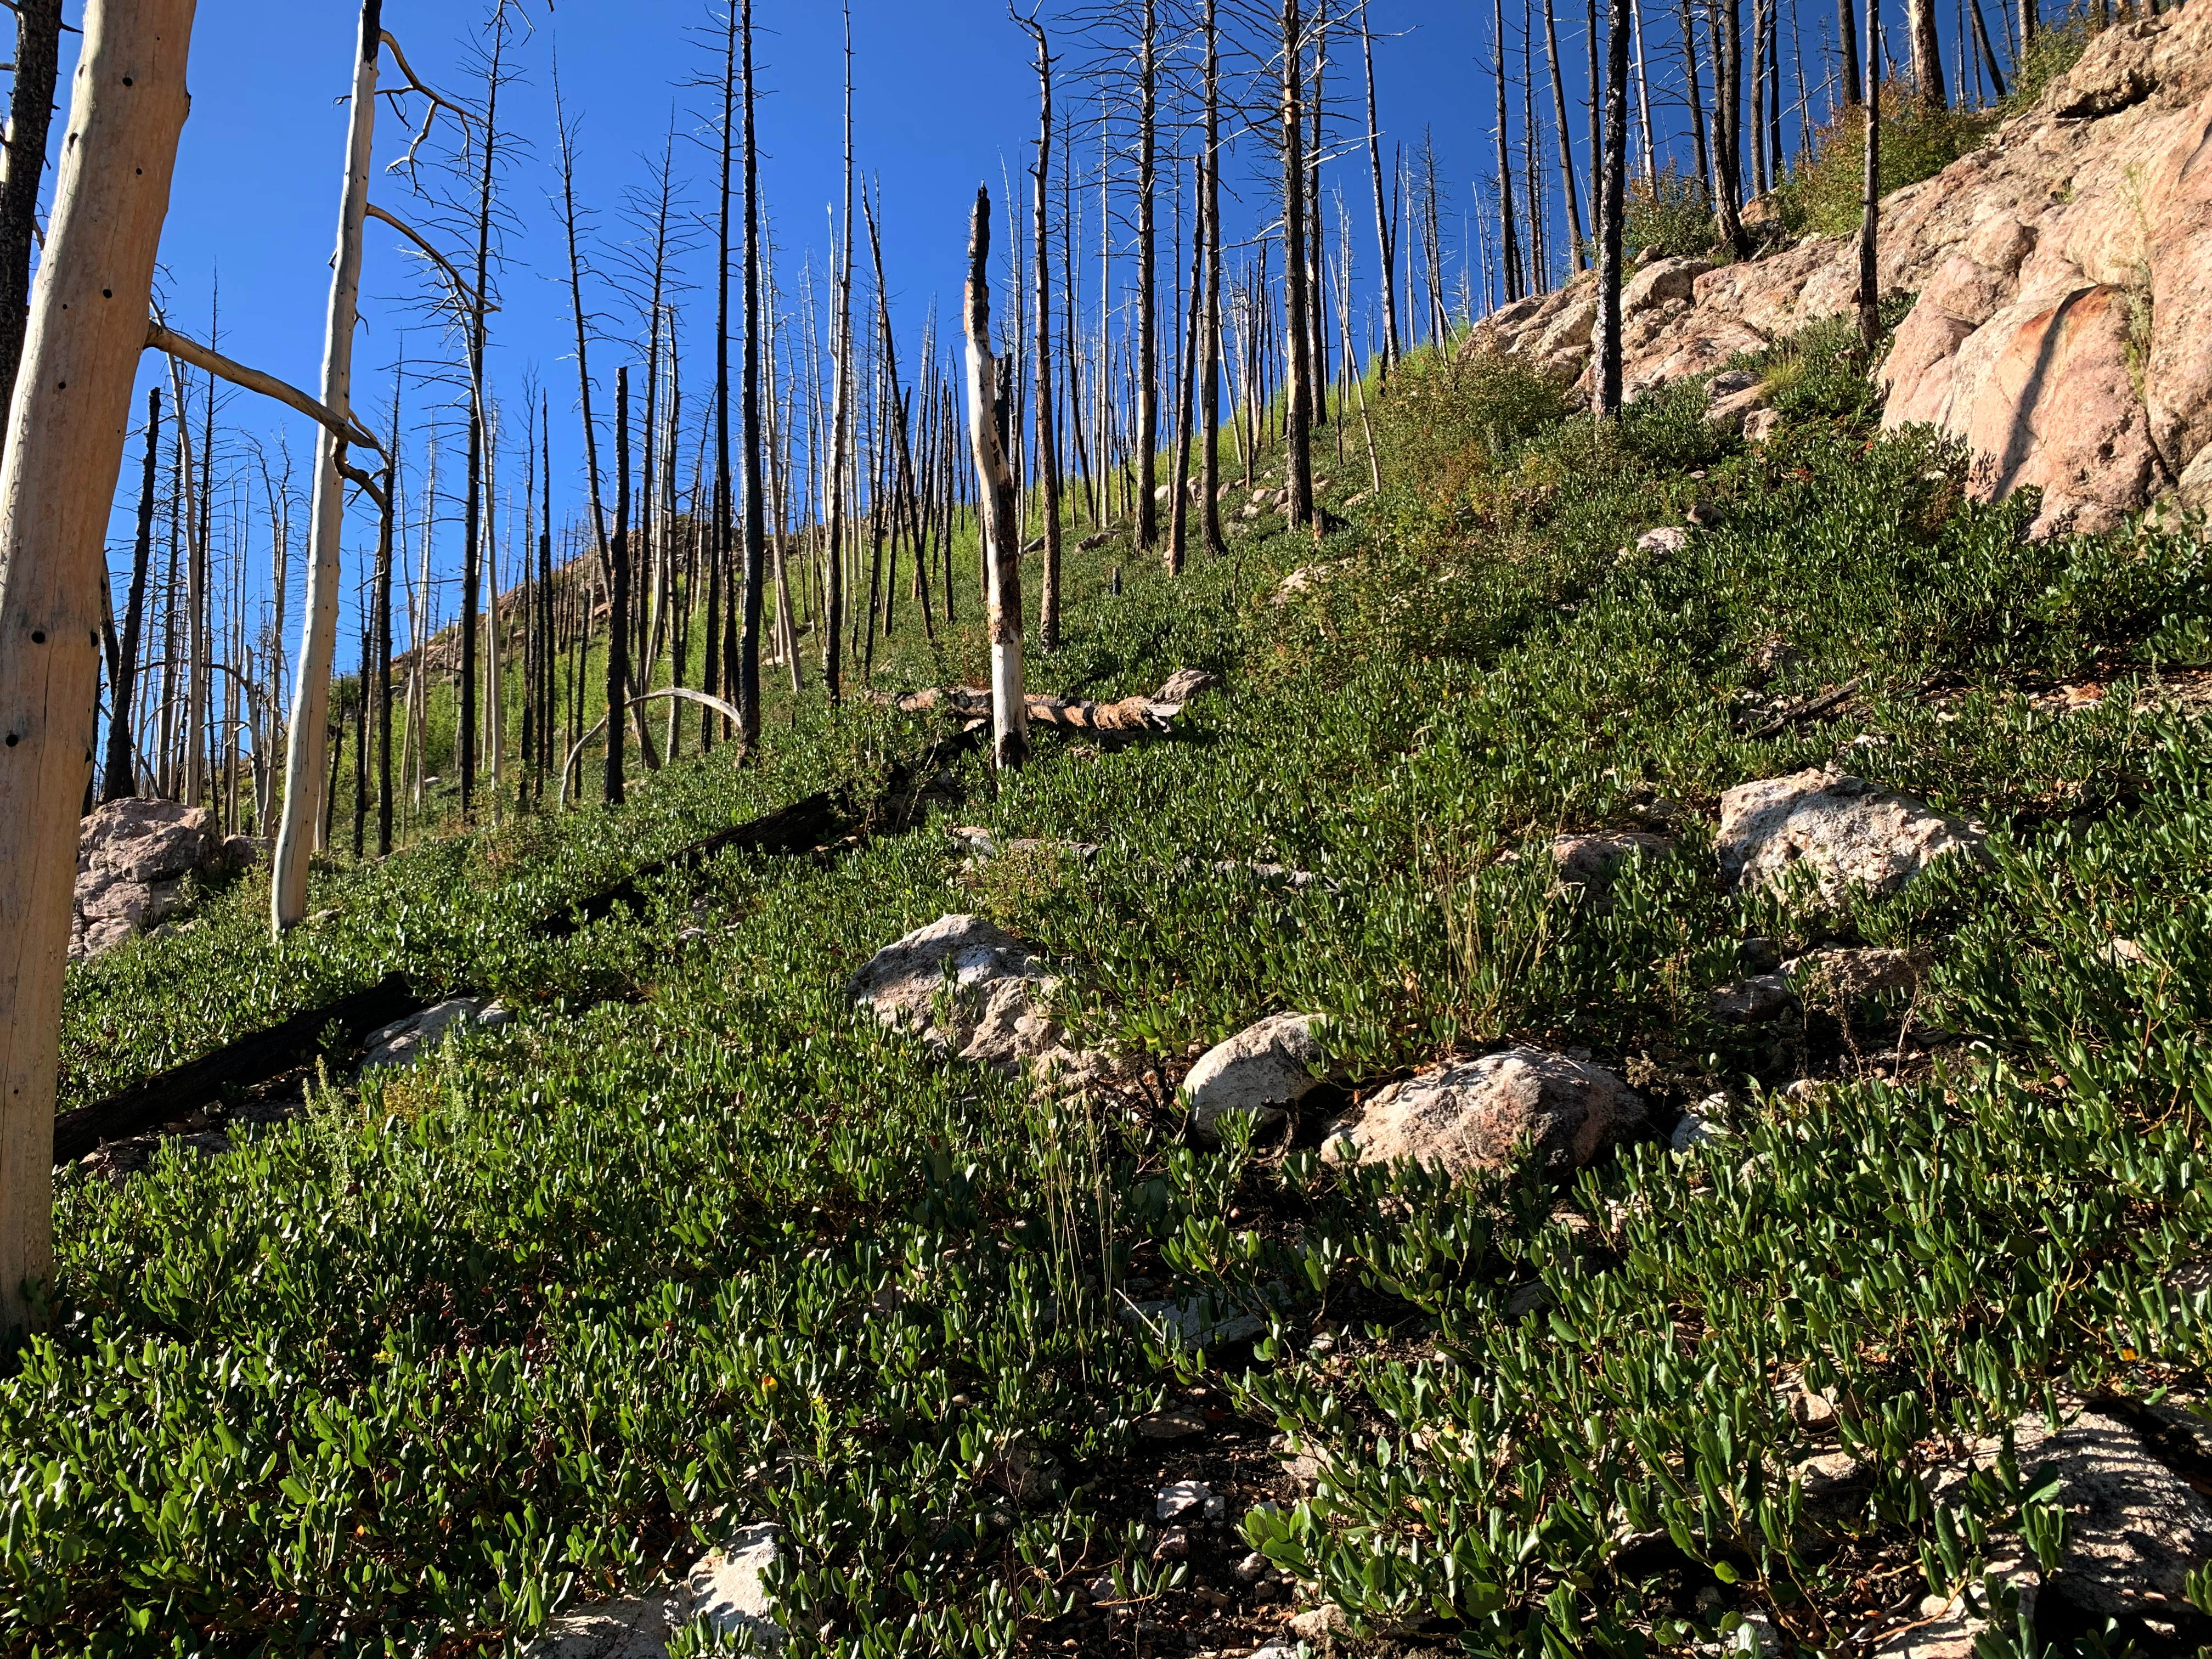
\includegraphics{../Images/ceonathus} \caption[Ceonathus]{Ceonathus growing in thick patches in a previously densely forested area severely burned by the Cameron Peak Fire. Photo by author.}\label{fig:figureTitle16}
\end{figure}

One community member lost a home in their family since 1945, a cabin which was also historically significant in the settler history of the Poudre. He similarly spoke about the cycle of grief within the context of nature's cyclical patterns.

\begin{quote}
\ldots Part of grieving is internalizing the memories, which is also letting them go. And so, in a sense, that can leave things unresolved. Because part of what you're dealing with in this whole business is how do we deal with grief, as well as how do we deal with life. \ldots To turn it around, it's as if you're experiencing nature's traumas. Because we sort of take nature for granted, even with the sense of the mystery. And then all of a sudden it looks as if it's all gone, but the mystery continues. Because it's coming back to life in its own way (C, 11/17/23).
\end{quote}

In another example of synergism across the three groups, a longtime wildland firefighter echoed similar sentiments.

\begin{quote}
As we go along, we learn that that is just the nature of living, right? It's that things break down, and change, and we are never perfect, and so we just have to be able to\ldots accept that imperfection, and work with it in the best means we can, versus getting hung-up on\ldots this isn't ideal, that we hold in our hearts and in our minds, as\ldots the way things should be (P, 3/3/23).
\end{quote}

Living and working in and studying wildfire-affected landscapes can provide opportunities to observe dynamic changes in vegetation, in hydrology, and in geologic movements that open different temporal windows on landscape processes. For people across the three groups, situating dramatic and traumatic wildfire-related experiences within the context of different life cycles of the material world helps reconcile these experiences as existing within patterns and timeframes beyond our human attachments.

\subsubsection{What Do We Value?}\label{what-do-we-value}

Scientists studying the interaction between wildfires and watersheds and forest regeneration, in particular, as well as some practitioners, identify certain challenges associated with more extreme wildfires and their repercussions, also within the context of climate change. These challenges include, among others, water quality and supply and whether certain tree species will be able to regenerate within the current climate and following high severity fire. Participants suggested a values-based approach in determining how we move forward as a society in addressing these challenges, such as this fire ecologist:

\begin{quote}
In thinking about what are the good or the bad things about fire, it's\ldots what're the human values that\ldots I ascribe to a place, like I think of this place as a ponderosa pine forest. Well, if that's what you want, then you can view it as bad or decide you need to take some action to try to re-initiate a forest like that if it's not gonna come back naturally. \ldots I think a lot about\ldots climate adaptation and what adaptation strategies we should be doing in post-fire and even pre-fire areas to prevent that next fire. And I think a lot of it does come back to\ldots what is it that we want from that ecosystem, or how do we want that ecosystem to thrive? Because no, I don't want\ldots a landscape to be replaced by all invasive species. But if it's a truly a functioning native community, then who am I to say that it should be a ponderosa pine forest instead of a grassland ecosystem if that's what's coming back naturally? But that's really hard\ldots to think about, when you're used to it being a forest or this specific type of forest (SU, 1/19/23).
\end{quote}

A forest ecologist also spoke about our predisposition to value the landscape in ways that are human-centric.

\begin{quote}
If you walk through a forest, and you come to an opening, the foresters think\ldots oh, here's a gap in the forest. Something happened here. We ought to have some trees here. But if you're a deer walking through the forest, you think, oh, thank God, I get something to eat. And so for a broad perspective on the forest, when you come out of the trees and into a meadow, it's the presence of something really, really good. It's a meadow. But if you've got this real bias towards trees, well, then it's just an absence of an opportunity where you could have had trees. So we may put some values in our hearts about forests versus meadows, but I don't think nature has those kinds of values. And if you're elk, you really like these fires. And if you're a woodpecker, you like the fires for at least 10 years afterward because that's all the food you want. But we have some choices if you'd like the landscape to be a little more like this, or make sure it doesn't go more like that. We can talk about what would be undesirable, what tools do we have in our toolkits to move away from those undesirable risks (SU, 8/3/23).
\end{quote}

A watershed scientist spoke about how she might identify areas of concern, connecting the presence of trees in watersheds to protecting water supply and quality.

\begin{quote}
\ldots sometimes it's hard to feel like going to plant a few trees here is really gonna make a difference\ldots so, I think that deciding what to do should be really focused on identifying those potential breaking points of the system\ldots those conditions where you no longer have enough water for the water supply, or your water quality is chronically impaired, and trying to figure out how to mitigate those tipping points (SU, 9/12/23).
\end{quote}

A wildfire policy analyst and former wildland firefighter expressed the need to expand dialog around how we talk about living with fire.

\begin{quote}
Plenty of people are traumatized by fire. And sure, we can talk about coexisting, but they lost so much of their livelihood or their house to it that it's\ldots difficult for them to even get there, which is also understandable. \ldots I think just having more emotional conversations about where we are at, and what fire means to us and could mean to us is the only way we're going to be able to shift how we live with fire (PN, 8/1/23).
\end{quote}

In the midst of ecological uncertainty wrought by conflagrations, especially in light of climate change, participants suggest that as a society, we both have to accept changing conditions and identify, based on what we value, those places where we can influence the trajectory of change. These insights offer guidance for policy makers, in thinking about how to adapt to changing condition and cultivating moral responsiveness (\citeproc{ref-whyteCrisisEpistemology2021}{K. Whyte 2021}) and values-based prioritization.

\subsection{Discussion}\label{discussion-2}

In response to increasingly severe wildfires which negatively impact people's lives, what I have termed conflagrations, I have shown that people across different constituencies engage in processes of sensemaking. The basis of this research project is to ask: what is the capacity of people to understand landscape transformations in ways that can help inform how we manage uncertainty and risk in the future associated with more extreme wildfires, flooding, and climate change? My findings suggest that people undergo processes of recalibration in response to the social, ecological, and geological disruptions caused by conflagrations that open up different ways of knowing the environment and of connecting past, present, and future landscape changes. These processes enable participants to reflect on experiences and knowledge holdings regarding wildfires of the past, extreme wildfires of the present, matters of agency and control in relation to wildfire risk, emotional pain resulting from different kinds of loss, temporal reorientation toward the material world, and future-oriented pathways based on defined values.

Like previous scholars have shown, I also found that participants across all three groups, community members, practitioners, and scientists, experience solastalgia, a form of emotional distress associated with environmental changes that disrupt perceptions of temporal continuity (\citeproc{ref-albrechtSolastalgiaDistressCaused2007}{Albrecht et al. 2007}; \citeproc{ref-asklandLivedExperiencesEnvironmental2018}{Askland and Bunn 2018}). One person referred to this as the feeling of ``camping in your own backyard'' (SF, 11/21/22). What I also found, however, was that these feelings exist alongside and are sometimes tempered by practices of sensemaking which situate grief and loss within notions of impermanence, renewal, and mystery, and a perception of nature as agentive and simultaneously destructive and cleansing. The majority of my research participants, again across all constituencies, express acceptance of uncertainty and of lack of control in relation to wildfires and the forces of nature writ large, including climate change, though not all specifically mentioned the latter. My research validates what the disaster anthropologist Roberto Barrios has referred to as the post-disaster emergence of ``affective ecologies'' (\citeproc{ref-barriosGoverningAffectNeoliberalism2017}{Barrios 2017}: 6), the ways that people understand the material world through sensory and emotive experiences contextualized by cultural and political historicities.

Among the practitioners and scientists who indicated that we cannot continue to operate under the illusion that we are able to control wildfire --- for which there is agreement across the three groups --- and whose work or research suggests that forest regeneration is changing for certain tree species under climate change, lack of control is not necessarily associated with lack of agency. First, one way to adapt to changing climatic conditions and the ecological consequences of more extreme wildfires is to ``appreciate that landscapes do change over time. And the landscapes we've grown up with for the last few decades have not been that way for very long. And they very much won't be that way in the future'' (SU, 8/3/23). Locating the changes we observe and experience in landscapes today as a result of wildfire as entangled in the lifecycles of the material world beyond our human-centric timeframe is a form of adaptation and agentive thinking. We need policies, investments, and governance addressing conflagrations, disaster, and climate change which reflect this ``poly-temporal worldview'' (\citeproc{ref-bjornerudTimefulnessHowThinking2018}{Bjornerud 2018}). Second, we can exert agency in an atmosphere of uncertainty by focusing efforts such as fuels treatments, watershed restoration, or tree plantings where, defined on what we value ecologically and socially, we want to see particular outcomes. One participant explained, and wrote about, an inverse approach, where stakeholders define what undesirable conditions might be instead, focusing efforts on reducing the risk associated with those conditions (\citeproc{ref-matonisBenefitsUndesirableApproach2016}{Matonis et al. 2016}).

We live in a world in which extreme wildfires will surely continue to occur given local contexts of fuel, drought, heat, land use and management, and broader patterns of climate change. This paper shines a light onto processes of recalibration which shape our understanding and relations with the material world in a way that allows for broader temporal and ontological expansiveness in contending with conflagrations, post-fire flooding, and uncertain climatic futures.

\subsection{References}\label{references-3}

\clearpage

\section{Conclusion}\label{conclusion}

\emph{The World and Life Won't be the Same Again}

On a cold and blustery day in December 2022, I sat on a couch next to my grandfather's cousin who would turn ninety-two years old on Christmas Day. We were warming ourselves in front of the woodstove in my extended family's new house built just within the two year window mandated by our insurance company after our old house had burned in the Cameron Peak Fire. This house was in a different location because of flooding danger at the old homesite. One of my aunts sat in a rocking chair nearby. In a few days time, multiple other family members would arrive to celebrate Christmas together at the new house for the first time. This Christmas gathering was organized for Sarah Beth and for her cousin Shelley, also in her 90s. The two of them spent every summer of their childhoods at the old family house, in an era before electricity had been installed up the Poudre, when there were kerosene lamps and an ice box for refrigeration. Sarah Beth spanned all six generations of our family's tenure in the Poudre Canyon. She held a repository of cumulative memories and represented an enduring sense of belonging passed down from one generation to the next in my family. At the same time, that one person's lifetime could stretch across six generations extending over a total of nearly 130 years was an indication of how shallow my family's history is in the Poudre, relative to Indigenous peoples who moved through this canyon for hundreds if not thousands of years (\citeproc{ref-burrisPeoplePoudreEthnohistory2006}{Burris 2006}) and to the ecological and geological timescales of this landscape made more noticeable by fire and flooding. I asked Sarah Beth what it was like for her losing the old home and seeing the changes to the land as a result of the wildfire.

``Things don't stay the same forever. \ldots kind of the hope there\ldots there's still something to come. It'll be different. History and good things don't come to an abrupt end. They evolve into something different. Almost as big a change as the wildfire to the countryside is all the buildings along the way coming up now. It used to be none of those would be there and that made it very different. \ldots I guess in some ways it's the impermanence of life and things in places and just {[}being{]} thankful when that's not the end, something else comes along.''

In this concluding chapter, I reflect on the themes represented by Sarah Beth's enduring sense of belonging and reckoning with large-scale loss and change.

\subsection{Insights and Reflections}\label{insights-and-reflections}

Building on previous theorizations of landscape and disaster in anthropology and social science scholarship on wildfire more broadly, this dissertation introduces new contributions in understanding the social, ecological, and political trajectories of wildfire. Drawing on over two years of ethnographic research involving participant observation, semi-structured interviews, and a landscape-based methodology incorporating walking conversations and go-alongs, this dissertation explores the following research questions: how do people make sense of large-scale landscape transformations and affective dimensions of loss and change wrought by wildfire and post-fire flooding; and how do people intersect with institutional responses to wildfire risk and recovery?

I offer three new insights as a result of my research findings. First, I introduce the concept of the social-ecological disturbance cascade to highlight how social consequences from wildfires, particularly in mountain watersheds, often emanate from the cascading ecological hazards that wildfires initiate. Conceptually linking social and ecological disturbances is important. Wildfire smoke is increasingly understood as extremely hazardous. For example, smoke from agricultural fires in Indonesia in 2015 is estimated to have caused over 100,000 excess deaths across Indonesia, Malaysia, and Singapore (\citeproc{ref-koplitzPublicHealthImpacts2016}{Koplitz et al. 2016}). Wildfire can also change the hydrological conditions of a watershed such that flooding, debris flows, and landslides are more likely for up to ten years following wildfire (\citeproc{ref-rengersLandslidesWildfireInitiation2020}{Rengers et al. 2020}). All of these watershed-related hazards have intersecting consequences for people's lives, both in areas where the wildfire occurred and downstream in the form of flooding, adverse water quality, or impacts to drinking water infrastructure. While ecological disturbances from wildfire are anticipated and constitute an active area of research, accompanying longitudinal social impacts are less understood and not as easily quantified. Accounting for multiple hazards across diverse jurisdictions and time horizons, and the complex and enduring ways people's lives are affected, can help to reshape mechanisms for response and recovery to support the range of social and ecological disruptions associated with wildfire.

Second, I propose centering co-stewardship with and agency for communities in cultivating practices of living with fire. I challenge certain prevailing narratives, revolving around the personal responsibility of those who live in the wildland urban interface (WUI) to follow best practices to reduce wildfire risk around their homes. I argue that the language of personal responsibility and the widespread use of the term WUI are counterproductive to reducing risk and can be divisive in a few key ways. One, the idea of the WUI artificially separates those who live in flammable landscapes from those who do not, even though our assumptions about what constitutes a fire-prone landscape have been challenged in recent years by, for example, the largely suburban Marshall Fire in Colorado and the fire which tore through the town of Lahaina in Hawaii. Assumptions about the WUI obscure local cultural, political, and ecological contexts of wildfire risk and craft a singular idea of community wildfire exposure and the reasons behind it.

Two, the concept of the WUI reinforces an understanding of wildfire as contained within the perimeter of the burn area, ignoring the very real danger of wildfire smoke, which can affect places thousands of miles away, and post-fire flooding, which can impact communities and water quality many miles downstream from a fire. My research adds to existing scholarship on multi-hazard planning approaches (\citeproc{ref-eatonWeFightAlberta2023}{Eaton and Shneiderman 2023}; \citeproc{ref-thompsonCapturingCascadingConsequences2024}{Thompson et al. 2024}) that recognizes the importance of attending to the full scope of how cascading hazards can be linked both socially and ecologically. I encourage a reconceptualization of those who live in fire-adapted landscapes as potential stewards rather than as agents of risk in co-producing strategies for living with fire. Living with fire is a process, in which individuals, communities, and governments are engaged, and only ever more so, as we reorient toward a world with more extreme wildfire. Expanding our understanding of geographies of risk could help communities better prepare for the multiple hazards associated with wildfire, and also assist policymakers and governments to identify infrastructure gaps for improved integrated response.

Third, my research shows that people who live with, study, and work in fire engage in processual sensemaking in response to extreme wildfire and the large-scale environmental changes that result from it. Cumulative sensemaking helps people recalibrate their relationship with landscapes affected by fire and post-fire flooding and debris flows, helping people to cope with affective and environmental disruptions. I found that among participants there is widespread acceptance of our inability to control fire, in spite of the fact that society operated for a long time as if it were something we could indefinitely control. Post-fire, a perception of nature as agentive and powerful shapes people's understanding of fire and flood as ecological forces. My research indicates that for people intimately affected by disaster, recognizing ecological patterns and lifecycles within the destructive forces of fire and flood helps configure meaning out of the loss and change caused by them. This method of recalibration, intentional or unintentional, is a form of adaptive and agentive thinking that connects the ``consequential materiality'' (\citeproc{ref-kosekUnderstoriesPoliticalLife2006}{Kosek 2006}: 23) of the past with the present and future. I argue that broadening our temporal horizons associated with the material world can help us better prepare for, respond to, and to some degree, accept ecologies of impermanence.

\subsection{Theoretical and Methodological Contributions}\label{theoretical-and-methodological-contributions}

My dissertation contributes to theoretical frameworks in anthropology, geography, and Indigenous Studies on temporality, materiality, and disaster. I build on these three sets of literatures through the lens of landscape, inspired by Tsing, Ingold, and Cresswell (\citeproc{ref-tsingWhenThingsWe2019}{A. Tsing 2019}; \citeproc{ref-ingoldBeingAliveEssays2011}{Ingold 2011}; \citeproc{ref-cresswellLandscapeObliterationPractice2003}{Cresswell 2003}), who observe and immerse themselves in the material formations of the landscapes in which they conduct research. I contribute to a theoretical and methodological engagement with landscape as a means by which to understand the material entanglements of wildfire. Through ``noticing landscapes'' (\citeproc{ref-tsingPatchyAnthropoceneLandscape2019}{A. L. Tsing, Mathews, and Bubandt 2019}) in the context of wildfire and post-fire watershed impacts, I encourage an expansion of the temporal and geographic frames through which society and governments prepare for, respond to, and recover from wildfire disturbance cascades. I introduce the concept of a social-ecological disturbance cascade to signify the linkages between the cascading hazards emanating from wildfire's footprint in a culturally molded environment with their consequences for the human and more than human lives inhabiting that environment.

This dissertation builds on critical resilience and vulnerability approaches in disaster anthropology (\citeproc{ref-barriosResilienceCommentaryVantage2016}{Barrios 2016}, \citeproc{ref-barriosGoverningAffectNeoliberalism2017}{2017}; \citeproc{ref-hoffmanCultureCrucialFactor2015}{Hoffman 2015}; \citeproc{ref-adamsMarketsSorrowLabors2013}{Adams 2013}). I show how, following the Cameron Peak Fire, as in other post-disaster contexts, people were subject to technocratic processes and political time (\citeproc{ref-zeeHoldingPatternsSand2017}{Zee 2017}) by capitalist-driven institutions (\citeproc{ref-kleinShockDoctrineRise2008}{Klein 2008}) and the state in navigating insurance claims, rebuilding, and additional hazards, such as the removal of a bridge following damage by the Black Hollow debris flow. I also discuss how wildfire preparedness efforts are embedded in institutionalized, state-driven, bottom-up governance practices ascribing individual responsibility for risk reduction and prescribing the manner in which risk reduction can take place and the resources made available to implement such efforts. Wildfire risk reduction efforts target individuals and sometimes blame them for exposing themselves to wildfire by choosing to live in hazardous landscapes. I identify that settler colonial expansion facilitated by federal legislation continues to shape contemporary settlement patterns in fire-adapted landscapes and that the history of federal forest management contributes to wildfire risk in places like the Poudre Canyon. This dynamic has long been critiqued in the context of environmental degradation (\citeproc{ref-guthmanRepresentingCrisisTheory1997}{Guthman 1997}) and more recently in relation to climate change adaptation (\citeproc{ref-nightingalePowerPoliticsClimate2017}{Nightingale 2017}; \citeproc{ref-chakrabortyMountainsInequalityEncountering2023}{Chakraborty, Rampini, and Sherpa 2023}) in the Global South. My research contributes to the still limited scholarship highlighting similar state-citizen relationships in wildfire preparedness and recovery practices in the Global North.

Another important contribution from disaster anthropology and those researching dramatic and often traumatic environmental changes is in identifying the affective dimensions of coping with the devastation of the ``built, natural, and social environments'' (\citeproc{ref-barriosGoverningAffectNeoliberalism2017}{Barrios 2017}: 5) emergent in post-disaster contexts (\citeproc{ref-asklandLivedExperiencesEnvironmental2018}{Askland and Bunn 2018}; \citeproc{ref-fowlerEmergingEnvironmentalEthics2018}{C. T. Fowler 2018}). My research builds on this prior scholarship to examine the processual sensemaking practices in which community members, practitioners, and scientists engaged in the aftermath of the CPF, Colorado's largest wildfire to date, what Frida Hastrup refers to as the everyday ``process of theorising'' (\citeproc{ref-hastrupWeatheringWorldRecovery2011}{Hastrup 2011}: 8). This dissertation contributes to uncovering how people understand and manage loss and change in the context of different disasters, of wildfire specifically, and in situated landscapes. People who live in the Poudre Canyon, who study forests and watersheds and work in fire, have intimate relationships with the river and streams, the trees, certain geographic features, and the shape of the terrain itself. I suggest that people recalibrate their relationship to place and to the material lifeworlds contained within it through constructing meaning out of landscape changes rooted in an ecological understanding of those changes.

This dissertation also contributes methodologically to previous theoretical and empirical engagements with landscape (\citeproc{ref-tsingMushroomEndWorld2015}{A. Tsing 2015}; \citeproc{ref-carlsonAgenciesPresentLandscapemaking2022}{D. Carlson 2022}; \citeproc{ref-benderIntroduction2020}{\textbf{benderIntroduction2020?}}; \citeproc{ref-mathewsLandscapesThroughscapesItalian2018}{Mathews 2018}). I show how observations and movements on, through, and with human and more than human beings in a wildfire-affected landscape is critical in understanding the temporal and material configurations and agencies of the past and of a landscape becoming.

\subsection{Research Implications}\label{research-implications}

My research findings are situated in a particular landscape revolving around a small community of people who live and work in and study this environment. It is only one of sixteen communities impacted by the CPF, and it suffered disproportionately fewer structure losses relative to the total number lost throughout the fire perimeter. One may ask how and why research about such a small place, so few people, so few home losses, matters for larger conversations or policy discussions about wildfire, disaster, or climate change. The arguments I lay out in this dissertation reflect precisely why the experiences of people during and after the CPF in the context of their lives in the Poudre Canyon matter for how we think about, plan for, respond to, and recover from wildfires everywhere.

First, as I describe in Chapter 2, recovery programs emerging from quantitative assessments of wildfire impacts such as structure loss can obscure less visible, more complex consequences and limit our temporal and spatial perceptual horizons to certain time periods and geographies. This leaves us less prepared to assign resources for long term recovery. Through ethnographic engagement with the Poudre Canyon community and with those who conduct research and work as fire and emergency practitioners here, my research uncovers the complexities and enduring emotional and structural challenges of post-fire recovery. Conceptually incorporating the social-ecological disturbance cascade in planning and policy formulations would inform management decisions, allocate resources, and encourage cross-jurisdictional cooperation in responding to timeframes and impacts associated with multiple, cascading hazards radiating out from wildfire.

Second, the upper Poudre Canyon is an example of a community in the WUI which both aligns with and defies assumptions about those who live in what I prefer to call fire-adapted landscapes. Demographically, this is not a community that is growing in population nor one in which new homes are continuously being built. It is, however, located in a forested, largely federally managed landscape, much of it now burned. As I describe in the Introduction and in Chapter 3, the patterns of settlement here are primarily attributable to the expulsion of Indigenous peoples from this area combined with federal legislation encouraging settler expansion across the western U.S. Federal forest management policies over the last century shaped the contemporary composition of forests and the behavior of fire. Ethnographic attention to the political and environmental histories of specific places highlighting the heterogeneity of communities grappling with wildfire risk, preparedness, and recovery can help shape policy and management approaches that account for the complex realities on the ground in different ecological, climatic, and weather contexts.

Third, the Poudre Canyon as a rural, unincorporated area has a particular relationship to risk exposure and management and to cross-jurisdictional governance. This dissertation explores what it means to live on relatively small pieces of land under county jurisdiction surrounded by vast federally managed landscapes, governed primarily from afar, in the context of wildfire and post-fire flooding. In Chapter 3, I outline how risks and hazards intersect with jurisdictional complexity and land and water management practices in a place where: the forests are owned by the USFS; the water is allocated to downstream municipalities but governed in part by a federal Wild \& Scenic designation; the wildlife is managed by the state; wildfire is managed by the state but usually first by the fire district, followed by the county, unless the fire is on federal lands, in which case it is managed by the USFS; people and private properties are governed by the county, which also manages emergencies; and the highway running through the canyon is managed by the state. I also provide ethnographic context in describing how the only local government --- the Poudre Canyon Fire Protection District (PCFPD) --- and private landowners model important roles in risk management and land stewardship practices that benefit ecological systems and populations extending beyond the confines of the Poudre Canyon that could be applied elsewhere.

Fourth, attending to how people who have different kinds of relationships to the Poudre Canyon make sense of landscape-altering wildfire and post-fire flooding contributes to knowledge production guiding how we all might better understand the human and more than human materialities and temporalities of the world we live in and how we might cope with living in a more fiery world with all its repercussions.

\subsection{Future Research Possibilities}\label{future-research-possibilities}

This dissertation opens up a more expansive research agenda for ethnographic engagement with wildfire and its human and more than human entanglements (\citeproc{ref-martindaleEntanglementTinkeringStructural2009}{Martindale 2009}). In Colorado, the Southern Ute Indian Tribe and Ute Mountain Ute Tribe are the only Indigenous groups with reservations and governments headquartered in the state, in spite of a history of at least forty-eight tribes having lived in what is now called Colorado at some time in the past and with over 200 Tribal Nations currently represented just in the Denver metro area (\citeproc{ref-daleyLongDenverWas2023}{Daley 2023}). What do these histories mean for the legacies of land use practices in this state that continue to inform how people and ecologies interact with wildfire? And how do these histories help us understand the ways in which ``emergencies highlight constitutional habits, the patterns of public decision-making'' (\citeproc{ref-feltesCrisisColonialismConstitutional2023}{\textbf{feltesCrisisColonialismConstitutional2023?}}) in the context of wildfire and disaster?

In Chapters 2 and 3, I address the jurisdictional complexities of wildfire in a place like the Poudre and trace some of these complexities back in time to land use practices deriving from federal policies dispossessing Indigenous peoples of land and encouraging settler colonial inhabitance on those lands. How different governance regimes influence relationships between citizens and the state is a subject which merits broader explorations than I cover in this dissertation, particularly for rural, unincorporated communities, and a subject for which greater ethnographic research is important. The broad theme of governance in relation to rural, unincorporated areas and how this affects planning and management practices around forest, fire, and flood management is also germane to how disaster recovery manifests for people in these areas. Although one-third of people in the U.S. live in unincorporated areas (\citeproc{ref-riveraEquitableRecoveryUnincorporated2024}{D. Rivera, Breder, and Dodd 2024}), research on lack of local governance or the role of rurality in disasters is still somewhat limited (\citeproc{ref-riveraUnincorporatedUnderservedCritical2023}{D. Z. Rivera 2023}; \citeproc{ref-kapucuDisasterPreparednessResilience2013}{Kapucu, Hawkins, and Rivera 2013}) across disaster literatures writ large and as part of ethnographic research in particular.

Drawing on themes emerging from my research in the Poudre Canyon, I am interested in further explorations around the implications of being surrounded by federal land, managed for the public good, administered from afar, the governance of which invariably disproportionately affects those whose lives intersect with its borders. The geographer Jake Kosek examines this question in the context of a rural community in northern New Mexico (\citeproc{ref-kosekUnderstoriesPoliticalLife2006}{Kosek 2006}) where land grants dictated the prescription of lands as communal for certain communities but where over time, the USFS managed to fold these lands under federal jurisdiction. His work, and the question of how communities are impacted, in both positive and negative ways, by living in proximity to federal public lands, was made all the more relevant in 2022 when two fires started by the USFS merged to become New Mexico's largest wildfire decimating the same rural, northern New Mexico communities Kosek wrote about sixteen years before. It also points to the importance of illuminating local geographic, ecological, political, and social contexts, highlighting how ethnography can contribute to policy planning and governance discussions. Speaking to the question of jurisdictional complexity in governance practices, what does it mean for critical infrastructure such as private bridges, originally privately and affordably built, to be subject to contemporary county and federal regulations rendering their ongoing maintenance or replacement unaffordable, as in the case of the Poudre Canyon? And how does disaster planning and recovery intersect with this reality?

Because we are deemed to be in the middle of a ``wildfire crisis'' (\citeproc{ref-forestserviceConfrontingWildfireCrisis2022}{F. Service 2022}) by the U.S. Forest Service's own estimation, what does this say about the capacity of this agency to effectively manage forests and fire? The archeologist Bruce Trigger writes that ``what pass as historical traditions are often mythical charters explaining and validating current social relations and these change as social relations change'' (\citeproc{ref-triggerNativesNewcomersCanadas1985}{Trigger 1985}: 167). Historians such as Stephen Pyne (\citeproc{ref-pyneFireAmericaCultural1997}{Pyne 1997}) and Jan van Wagtendonk (\citeproc{ref-vanwagtendonkHistoryEvolutionWildland2007}{van Wagtendonk 2007}) have both written about the history of the USFS and wildfire management in the U.S. There remains a role, however, for anthropological research in picking apart how to understand the purview of an agency like the USFS in relation to the trajectory of its landscape ideologies over time and how its competing interests --- timber sales versus thinning and prescribed fire for ecological and fire risk reduction purposes, for example --- shape the outcomes of wildfire and forest management. Future research could examine the tensions inherent in an agency like the USFS illuminating where investments and policies need to change in order for this country to adequately prepare for the kinds of wildfires we are seeing today and to recover from them, both socially and ecologically.

In Chapter 3, I develop the idea of cultivating stewardship, of land and of fire, among communities who live in fire-adapted landscapes and criticize interactions with homeowners that rely on harmful narratives, such as the notion of personal responsibility. I make brief reference to Amy Johnson's term ``settlerism'' (\citeproc{ref-johnsonSettlerSensibilitiesEnvironmental2023}{A. Johnson 2023}), or the idea that landscapes are shaped by colonial settlement projects, which I have also alluded to here in the Conclusion. Part of the basis of my argument promoting a perception of people in the Poudre as potential stewards stems from learning during my fieldwork about the deep connections and care people in the Poudre have for the river, the forests, the wildlife, and for some families, to particular places named and routinely visited over multiple generations. There is an enduring and important relationship here with place, even though the existence of this relationship is born out of a violent past enabling the settlement of non-Indigenous peoples in the first place. At the Cross-Boundary Landscape Resilience Workshop I attended in May 2023, which was primarily about wildfire, I listened to the Tribal Projects Coordinator for the USFS speak on a panel. She said tribes need decision-making powers to determine their own pathway toward collaboration with other government entities and that tribal nations' interests cannot only be represented by numbers. Stories and relationships are what matter in creating resilient partnerships, she said, and criticized the transactional nature of collaboratives attempting to work with tribal nations in the U.S. In my notes from the workshop about this panel, I wrote, ``We can learn from these kinds of identifications and delineations and lessons around working with tribal communities. All communities' interests should be engaged through storytelling and relationships.'' What are the implications of mobilizing similar language and strategies for collaborating with Indigenous sovereign nations in order to highlight settler connections to landscapes and the meaning of these connections in developing land and fire stewardship practices?

Another interesting area of research for an anthropology of wildfire is in multi-sited ethnography examining wildfire narratives, land use practices, and ecological conditions in places with different cultural, political, and environmental histories. As I discussed in Chapter 3, entrenched assumptions exist regarding what is referred to as the WUI in the United States, and particularly in the western U.S., one of which is the idea that the `wildfire problem' --- or the `WUI problem,' such as it is called --- is constituted by the {[}increasing{]} presence of people in landscapes that burn. In areas of Mediterranean Europe, the wildfire problem is inversely characterized. It is agricultural abandonment and the absence of people in rural areas which is understood to leave them more susceptible to wildfire (\citeproc{ref-moreiraModellingImpactAgricultural2007}{Moreira and Russo 2007}). What can we learn about how people understand and live with wildfire risk in different parts of the world that can inform the futures we choose to create in a world with more fire and ever more uncertain climates?

There is much more to examine in relation to understanding what it means to live with fire. As I have drawn attention to in this dissertation, wildfire, like other disasters, exists in relation to other hazards. I have identified how practices encouraged as part of living with fire often do not address how to live with smoke as well as wildfire risk, for example, or with post-fire flooding. A multi-hazard relationship which I am particularly interested to explore further is that between extreme heat and wildfire, particularly in the context of wildfire risk reduction measures. What are the implications for places where people are simultaneously exposed to these hazards within their homes? The Home Ignition Zone which provides guidance on reducing wildfire risk in five, thirty, and 100 foot zones out from the house includes recommendations to cut down trees which may contribute to igniting a home or igniting other trees as a ladder fuel. How consequential is removing trees from near homes in terms of extreme heat exposure? How should we consider the role of air conditioning and power outages during wildfires and wildfire smoke exposure in providing guidance to homeowners to remove trees providing shade? How might existing inequalities be exacerbated by risk reduction measures which attempt to reduce one hazard but introduce another?

\subsection{Outro}\label{outro}

I attended a presentation in January 2024 by a landscape architect who, taking inspiration from Dutch perceptions of and designs considering water as a hazard, developed three strategies for cultivating practices of living in fire-affected and -adapted landscapes, characterized as defensive, resilient, and resistant (\citeproc{ref-gorskiBurntTaleThree2023}{Gorski 2023}). His designs were beautiful and innovative, incorporating ideas for trails that guide visitors through forest mosaics comprising recently burned, young, and mature forests with lookout towers and burnt memorials along the way. I thought of this as intentionally cultivating an aesthetic for burned landscapes, a way to encourage people to recalibrate their relationship with particular ecologies.

\begin{figure}
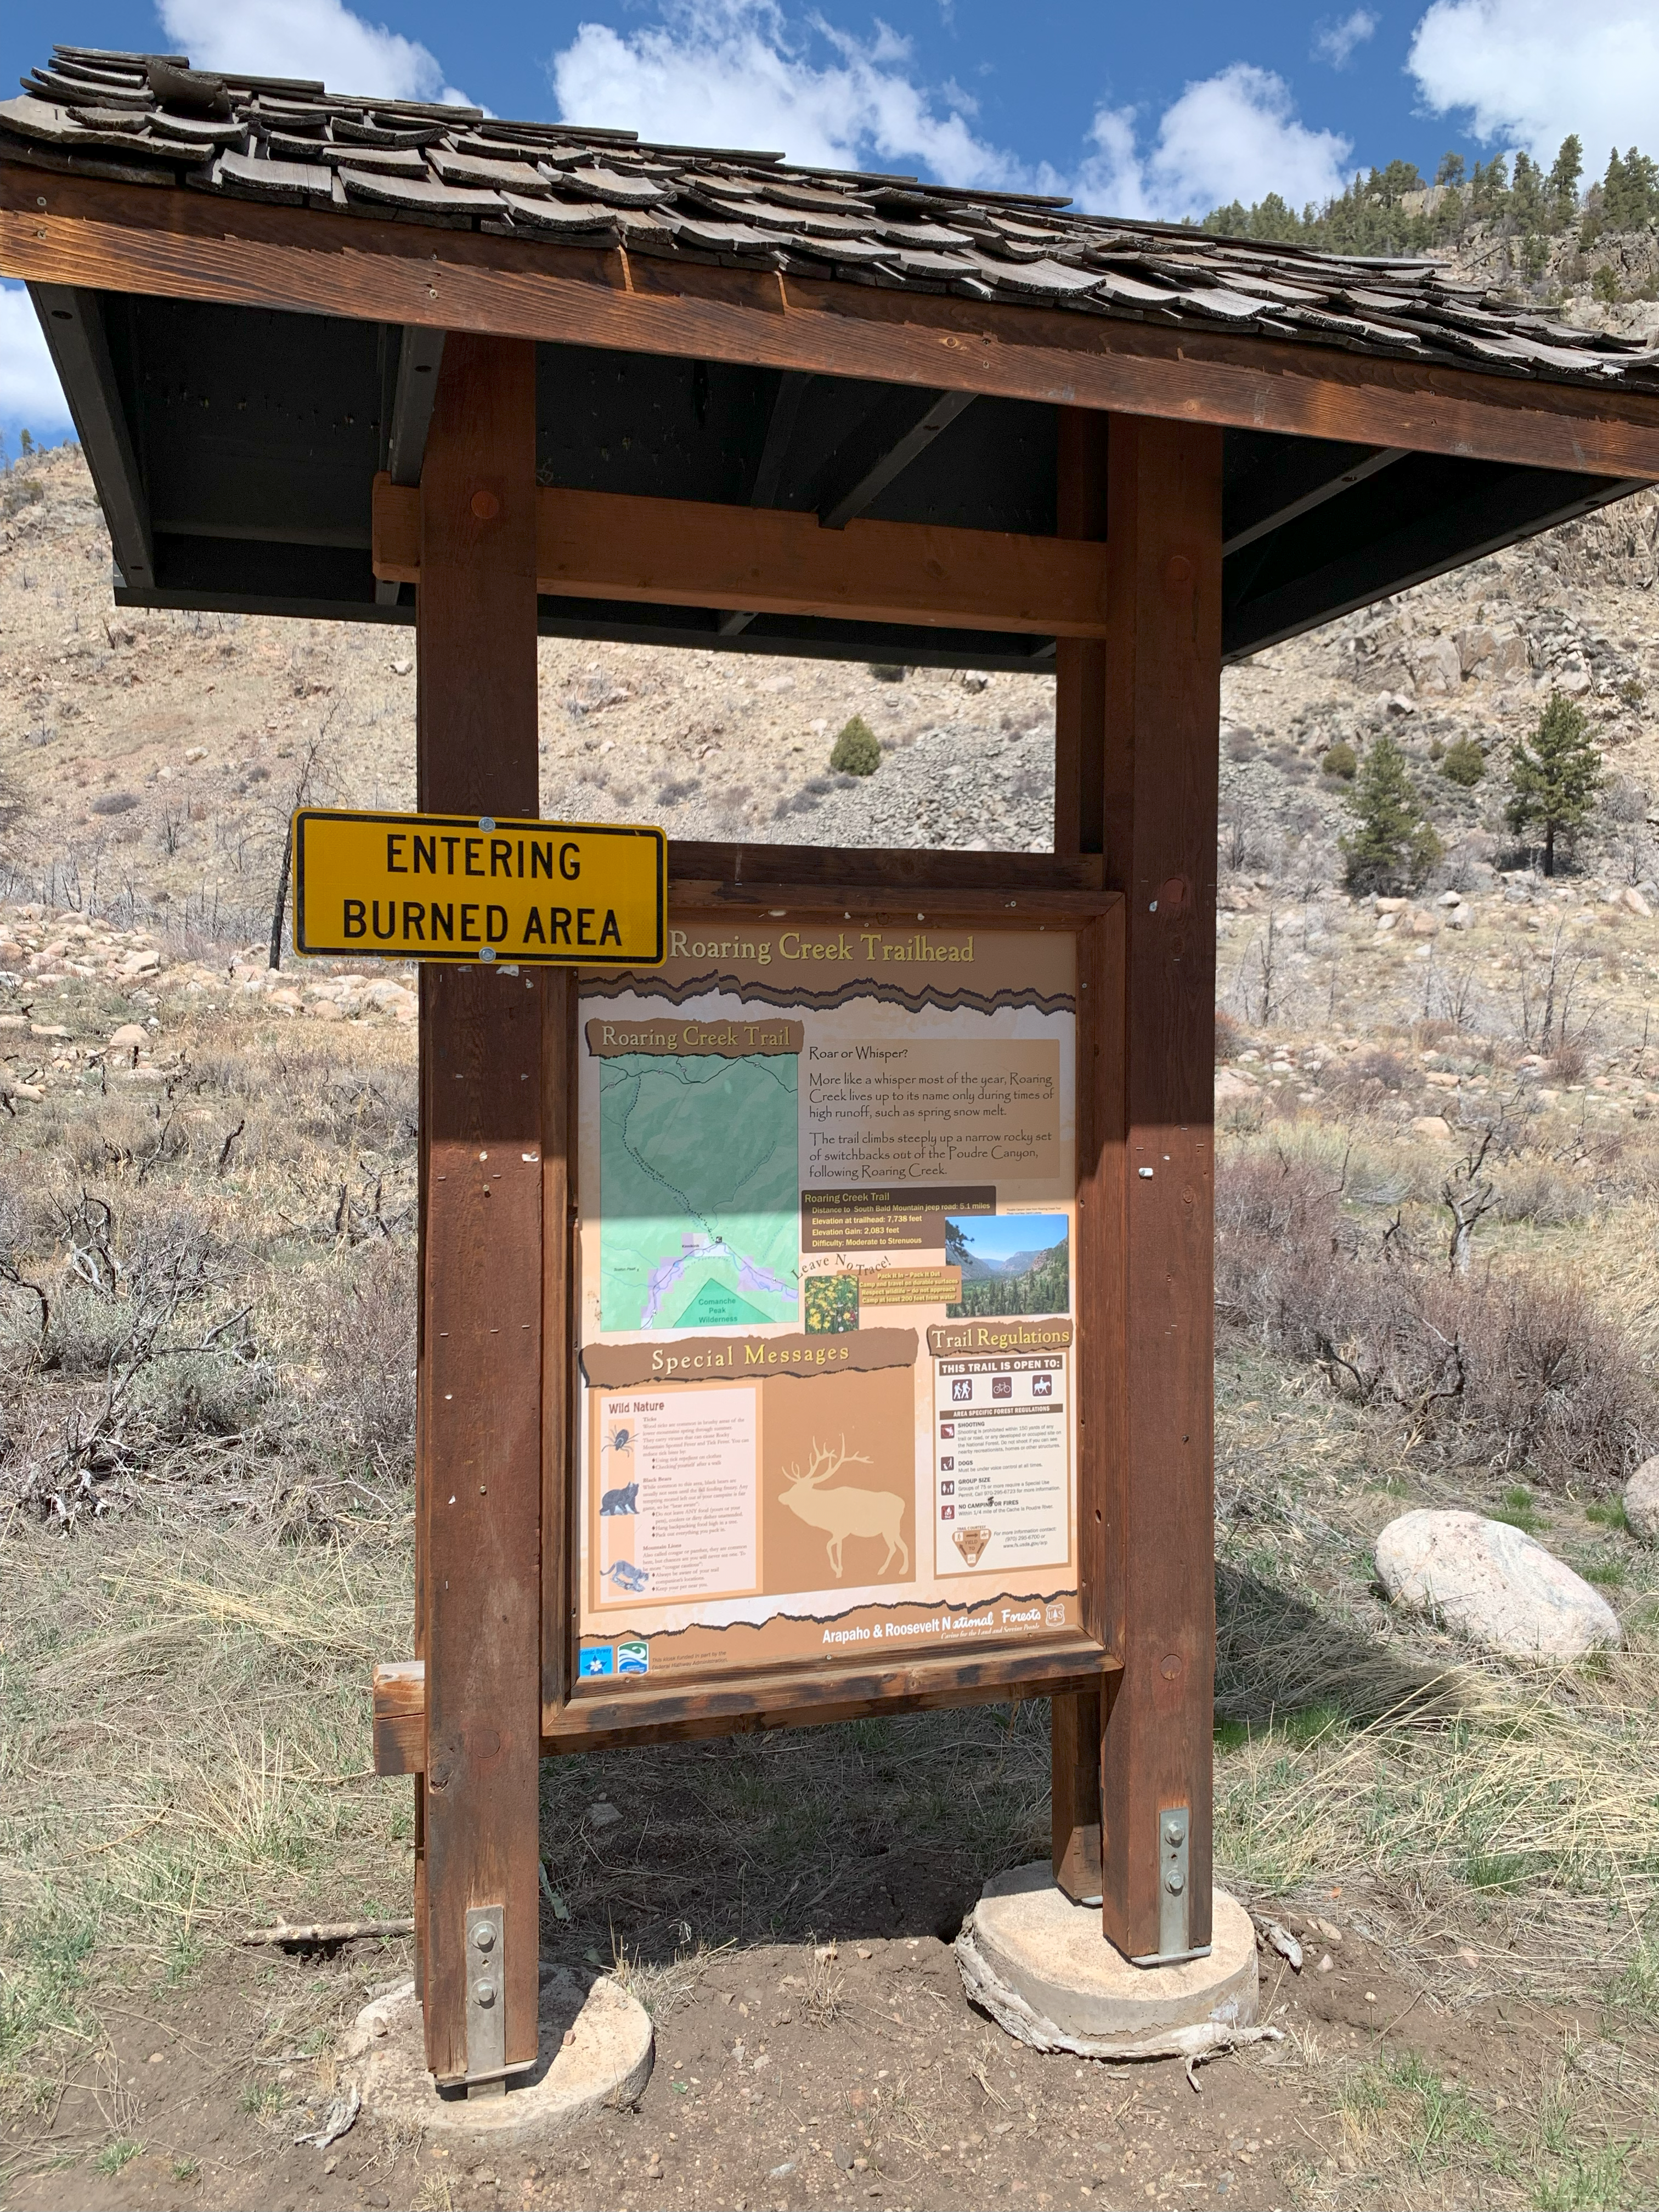
\includegraphics{../Images/trailhead} \caption[Roaring Creek Trailhead]{Typical U.S. Forest Service trailhead sign. Photo by author.}\label{fig:figureTitle17}
\end{figure}

Shortly after this, I went for a hike on a USFS trail that had been closed to the public for three years and had only been opened a couple months prior after sustaining damage from the CPF. USFS signs at trailheads here all follow a certain template. There is a map and description of the trail, information about what users are allowed on the trail, warnings about the presence of ticks, mountain lions, and bears, and an attached sign stating ``Entering Burned Area.'' I was dismayed to see that there was no information explaining the three year-long trail closure, the CPF, or anything contextualizing this scorched but regenerating landscape, such as a suggestion to look out for new lodgepole pine seedlings and the particular fire adaptation of serotiny in some lodgepole pines. Certainly, the USFS is experiencing both funding and staffing challenges that might explain the absence of any context at all, but it is reflective of a broader cultural and political lack of attention to the affective dimensions of living with fire.

\begin{figure}
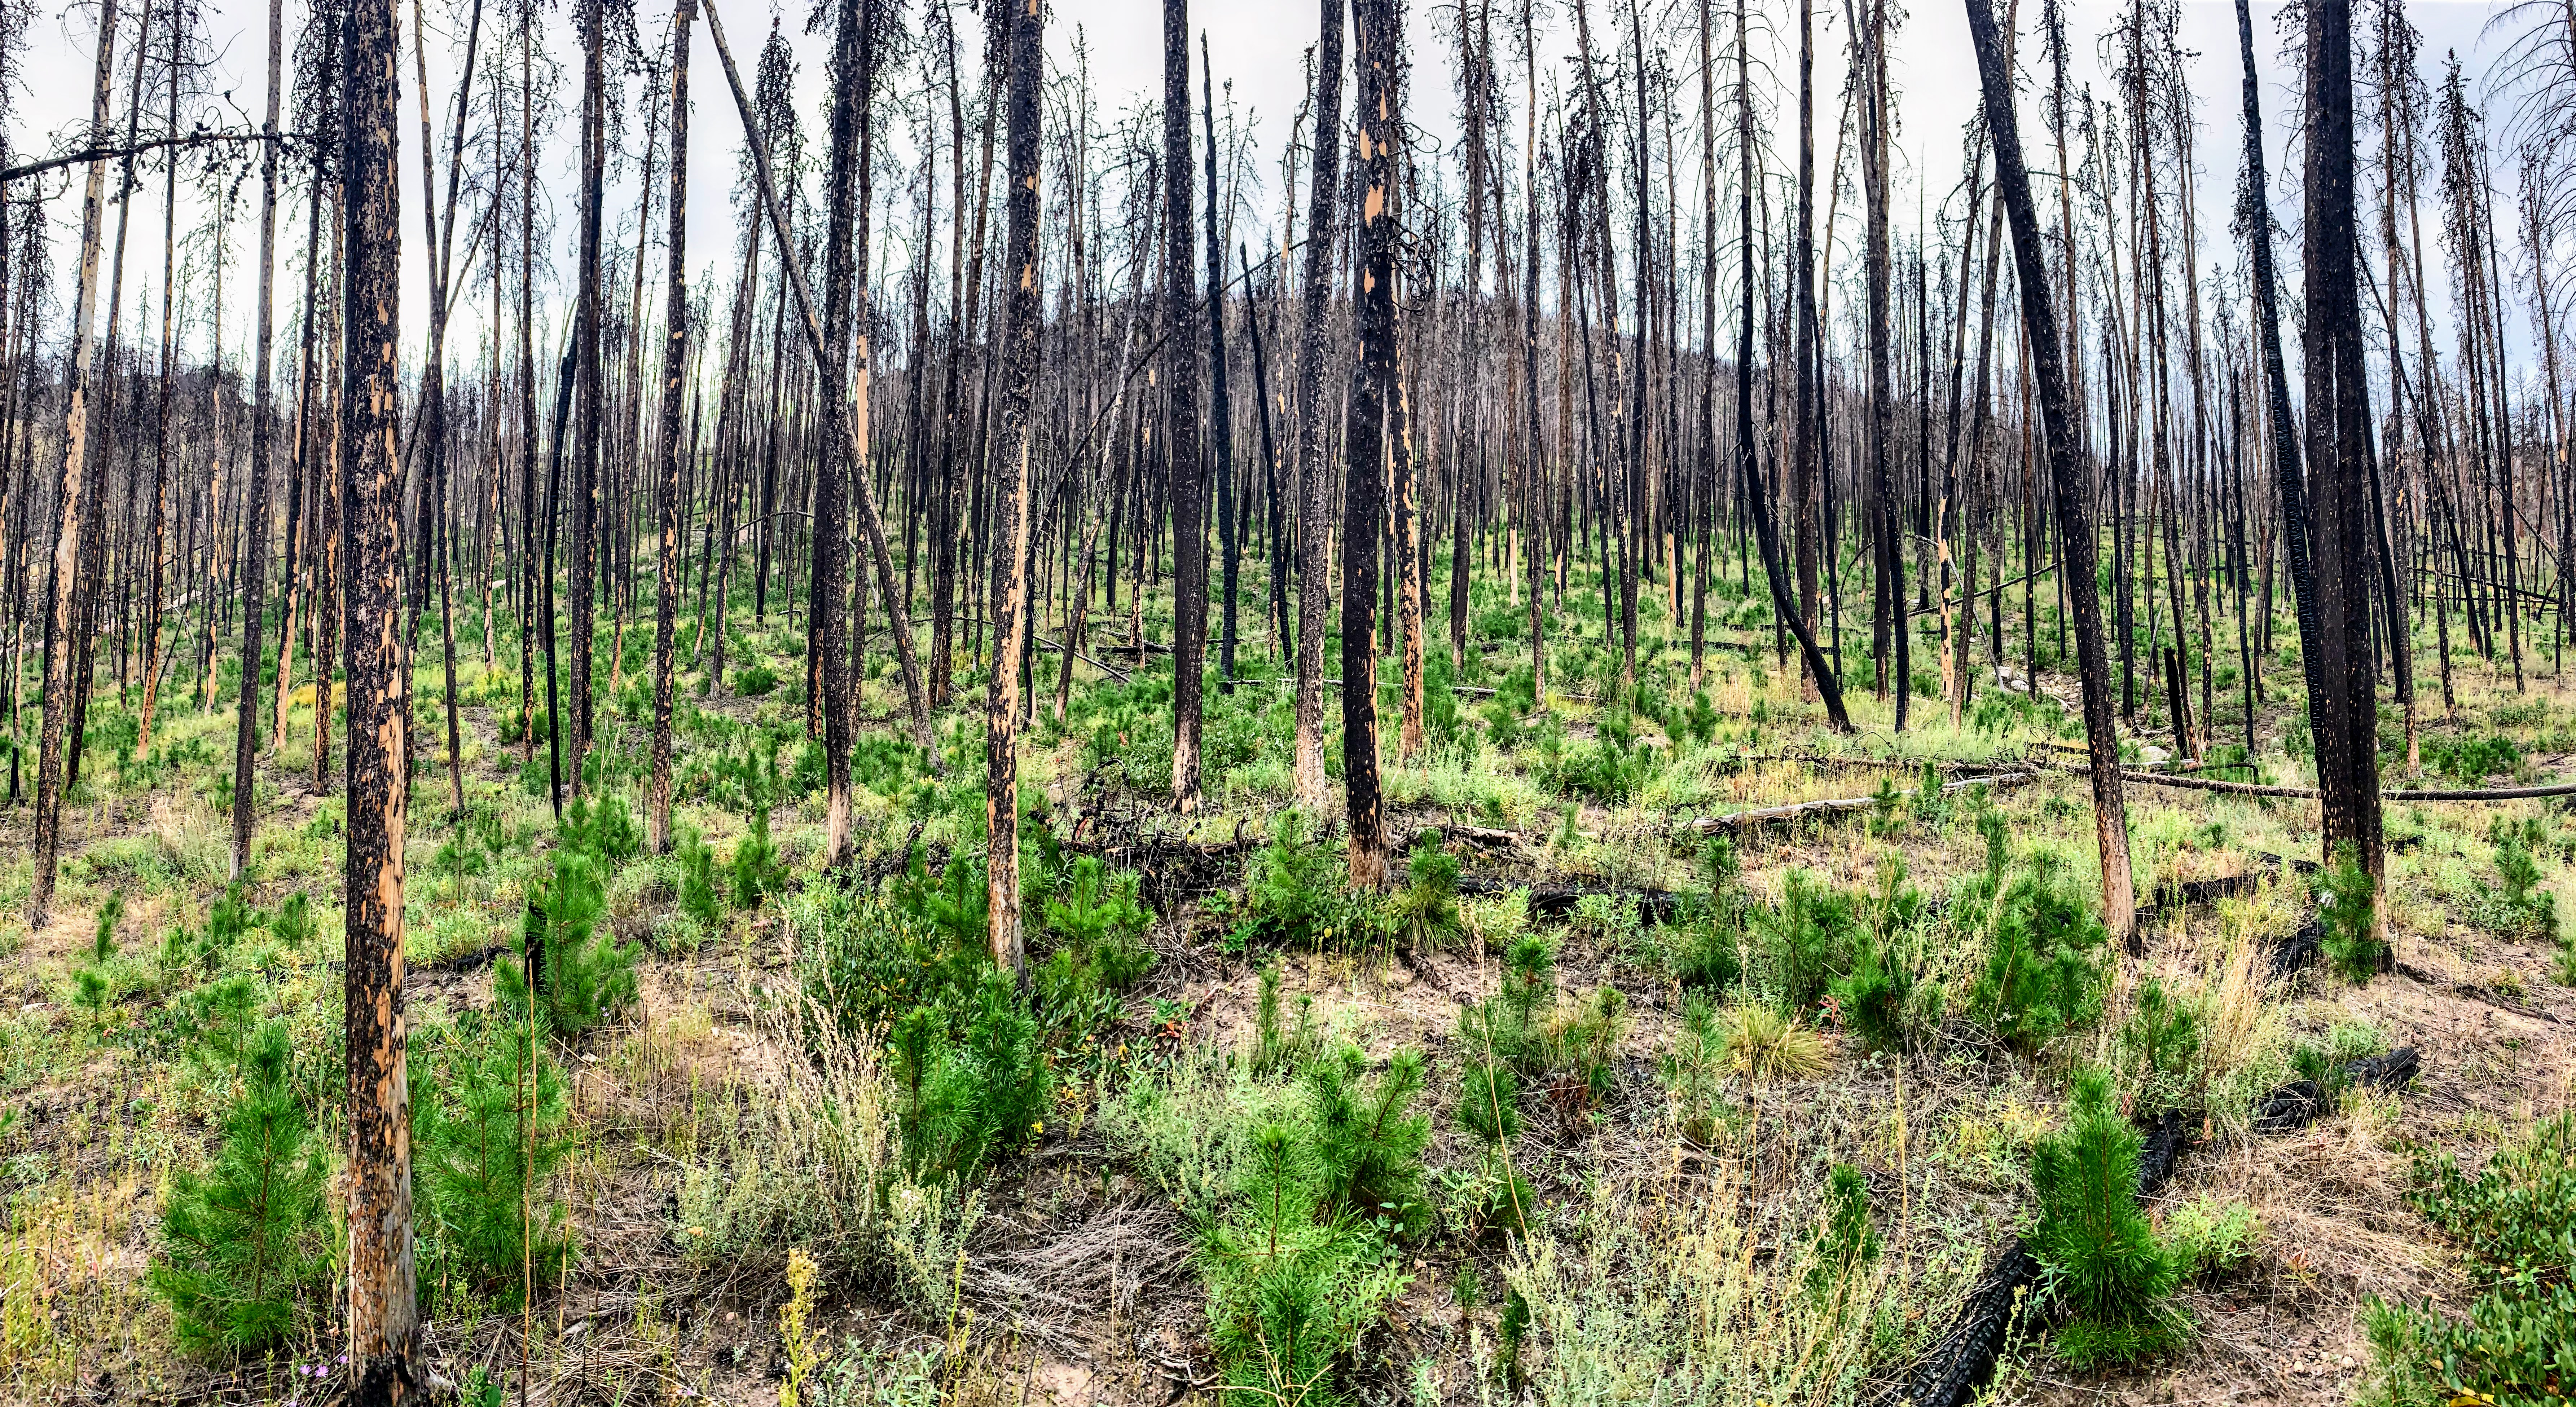
\includegraphics{../Images/lodgepole} \caption[Lodgepole pine]{Thriving lodgepole pine seedlings four years after the Cameron Peak Fire. Photo by author.}\label{fig:figureTitle18}
\end{figure}

This dissertation demonstrates that people come to terms with loss caused by the wildfire and associated hazards in part through an understanding of ecological patterns and possibilities. I advocate for further research considering how we might create pathways for normalizing and cultivating our relationships with burned landscapes and for assigning more resources at different jurisdictional levels to do so. This is another ripe area for further ethnographically engaged research. We are living in a world with more conflagrations, and learning how to cope with this reality is an ongoing process of recalibration, not just for communities but also for fire practitioners, emergency managers, and scientists. The task at hand is not just about living with fire, which people have been doing for a long time, but about living with potentially ecologically and socially devastating fire with long term repercussions for forests, watersheds, and people. At the same time, it is about cultivating an appreciation for the nuances of how fire moves across particular landscapes and interacts with different tree species, for example, which have adapted to fire over time in diverse ways, for some of which moderate to high severity fire may be within its historical range of variability. Individuals, communities, and governments need to prepare for and respond to fire and its accompanying hazards situated in a realistic understanding of the temporal and spatial scales of harm and loss while also contextualizing the regenerative, ecologically beneficial functions of fire and flood.

\section{References}\label{references-4}

\clearpage

\section*{Bibliography}
\addcontentsline{toc}{section}{Bibliography}

\noindent
\leftskip=2em
\parindent=-2em

\phantomsection\label{refs}
\begin{CSLReferences}{1}{0}
\bibitem[\citeproctext]{ref-20102020Census2022}
{``2010 to 2020 {Census Tract Population Change}.''} 2022. Tennesee State Data Center. \url{https://myutk.maps.arcgis.com/apps/instant/sidebar/index.html?appid=b6cf315a28aa4089873ee3442d4a2597}.

\bibitem[\citeproctext]{ref-abatzoglouCompoundExtremesDrive2021}
Abatzoglou, John T., David E. Rupp, Larry W. O'Neill, and Mojtaba Sadegh. 2021. {``Compound {Extremes Drive} the {Western Oregon Wildfires} of {September} 2020.''} \emph{Geophysical Research Letters} 48 (e2021GL092520). doi:\href{https://doi.org/10.1029/2021GL092520}{10.1029/2021GL092520}.

\bibitem[\citeproctext]{ref-zotero-10034}
{``About.''} 2024. \emph{Fire Networks}. Accessed June 27. \url{https://firenetworks.org/}.

\bibitem[\citeproctext]{ref-Us2024}
{``About {Us}.''} 2024. \emph{Poudre Canyon Fire District}. \url{https://pcfpd.specialdistrict.org/about-us}.

\bibitem[\citeproctext]{ref-abramSpellSensuousPerception1996}
Abram, David. 1996. \emph{The {Spell} of the {Sensuous}: {Perception} and {Language} in a {More-Than-Human World}}. New York: Vintage Books. \url{http://archive.org/details/the-spell-of-the-sensuous-perception-and-language-in-a-more-than-human-world}.

\bibitem[\citeproctext]{ref-adamsMarketsSorrowLabors2013}
Adams, Vincanne. 2013. \emph{Markets of {Sorrow}, {Labors} of {Faith}: {New Orleans} in the {Wake} of {Katrina}}. Durham: Duke University Press.

\bibitem[\citeproctext]{ref-adamsAnticipationTechnoscienceLife2009}
Adams, Vincanne, Michelle Murphy, and Adele E. Clarke. 2009. {``Anticipation: {Technoscience}, Life, Affect, Temporality.''} \emph{Subjectivity} 28 (1): 246--65. doi:\href{https://doi.org/10.1057/sub.2009.18}{10.1057/sub.2009.18}.

\bibitem[\citeproctext]{ref-adhikariGenderedConsequencesSocial2022}
Adhikari, Radha, and Jeevan R. Sharma. 2022. {``Gendered Consequences of Social Changes in {Nepal}: Rich Possibilities.''} \emph{European Bulletin of Himalayan Research}, no. 58 (July). Centre d'{é}tudes sud-asiatiques et himalayennes (UMR8077 CNRS/EHESS), Heidelberg University, University of London. doi:\href{https://doi.org/10.4000/ebhr.549}{10.4000/ebhr.549}.

\bibitem[\citeproctext]{ref-adlamKeepersFlameSupporting2021}
Adlam, Christopher, Diana Almendariz, Ron W. Goode, Deniss J. Martinez, and Beth Rose Middleton. 2021. {``Keepers of the {Flame}: {Supporting} the {Revitalization} of {Indigenous Cultural Burning}.''} \emph{Society \& Natural Resources} 0 (0). Routledge: 1--16. doi:\href{https://doi.org/10.1080/08941920.2021.2006385}{10.1080/08941920.2021.2006385}.

\bibitem[\citeproctext]{ref-ahmannItsExhaustingCreate2018}
Ahmann, Chloe. 2018. {``{`{It}'s Exhausting to Create an Event Out of Nothing'}: {Slow Violence} and the {Manipulation} of {Time}.''} \emph{Cultural Anthropology} 33 (1): 142--71. doi:\href{https://doi.org/10.14506/ca33.1.06}{10.14506/ca33.1.06}.

\bibitem[\citeproctext]{ref-ahmannBreathingLateIndustrialism2020}
Ahmann, Chloe, and Alison Kenner. 2020. {``Breathing {Late Industrialism}.''} \emph{Engaging Science, Technology, and Society} 6 (November): 416--38. doi:\href{https://doi.org/10.17351/ests2020.673}{10.17351/ests2020.673}.

\bibitem[\citeproctext]{ref-albrechtSolastalgiaDistressCaused2007}
Albrecht, Glenn, Gina-Maree Sartore, Linda Connor, Nick Higginbotham, Sonia Freeman, Brian Kelly, Helen Stain, Anne Tonna, and Georgia Pollard. 2007. {``Solastalgia: {The Distress Caused} by {Environmental Change}.''} \emph{Australasian Psychiatry} 15 Supplement (1\_suppl): S95--98. doi:\href{https://doi.org/10.1080/10398560701701288}{10.1080/10398560701701288}.

\bibitem[\citeproctext]{ref-allenLotsLightningPlenty2002}
Allen, Craig D. 2002. {``Lots of {Lightning} and {Plenty} of {People}: {An Ecological History} of {Fire} in the {Upland Southwest}.''} In \emph{Fire, {Native Peoples}, and the {Natural Landscape}}, edited by Thomas Vale, 143--93. Washington, D.C.: Island Press.

\bibitem[\citeproctext]{ref-asfawRoleSocialSupport2019}
Asfaw, Henok Workeye, Tara McGee, and Amy Cardinal Christianson. 2019. {``The Role of Social Support and Place Attachment During Hazard Evacuation: The Case of {Sandy Lake First Nation}, {Canada}.''} \emph{Environmental Hazards} 18 (4). Taylor \& Francis: 361--81. doi:\href{https://doi.org/10.1080/17477891.2019.1608147}{10.1080/17477891.2019.1608147}.

\bibitem[\citeproctext]{ref-asklandLivedExperiencesEnvironmental2018}
Askland, Hedda Haugen, and Matthew Bunn. 2018. {``Lived Experiences of Environmental Change: {Solastalgia}, Power and Place.''} \emph{Emotion, Space and Society} 27. Elsevier: 16--22. doi:\href{https://doi.org/10.1016/J.EMOSPA.2018.02.003}{10.1016/J.EMOSPA.2018.02.003}.

\bibitem[\citeproctext]{ref-awasisAnishinaabeTimeTemporalities2020}
Awasis, Sakihitowin. 2020. {``{"Anishinaabe time": temporalities and impact assessment in pipeline reviews}.''} \emph{Journal of Political Ecology} 27 (1). University of Arizona Libraries. doi:\href{https://doi.org/10.2458/v27i1.23236}{10.2458/v27i1.23236}.

\bibitem[\citeproctext]{ref-bakerIndiansFireRocky2002}
Baker, William L. 2002. {``Indians and {Fire} in the {Rocky Mountains}: {The Wilderness Hypothesis Renewed}.''} In \emph{Fire, {Native Peoples}, and the {Natural Landscape}}, edited by Thomas Vale. Washington, DC: Island Press.

\bibitem[\citeproctext]{ref-balchHumanstartedWildfiresExpand2017}
Balch, Jennifer K., Bethany A. Bradley, John T. Abatzoglou, R. Chelsea Nagy, Emily J. Fusco, and Adam L. Mahood. 2017. {``Human-Started Wildfires Expand the Fire Niche Across the {United States}.''} \emph{Proceedings of the National Academy of Sciences} 114 (11). National Academy of Sciences: 2946--51. doi:\href{https://doi.org/10.1073/pnas.1617394114}{10.1073/pnas.1617394114}.

\bibitem[\citeproctext]{ref-balchFastestgrowingMostDestructive2024}
Balch, Jennifer K., Virginia Iglesias, Adam L. Mahood, Maxwell C. Cook, Cibele Amaral, Amy DeCastro, Stefan Leyk, et al. 2024. {``The Fastest-Growing and Most Destructive Fires in the {US} (2001 to 2020).''} \emph{Science} 386 (6720). American Association for the Advancement of Science: 425--31. doi:\href{https://doi.org/10.1126/science.adk5737}{10.1126/science.adk5737}.

\bibitem[\citeproctext]{ref-baldwinSurvivingSixthExtinction2018}
Baldwin, Daryl, Margaret Noodin, and Bernard C. Perley. 2018. {``Surviving the {Sixth Extinction}: {American Indian Strategies} for {Life} in the {New World}.''} In \emph{After {Extinction}}, edited by Richard Grusin, 201--34. University of Minnesota Press. doi:\href{https://doi.org/10.5749/j.ctt22nmbq0.12}{10.5749/j.ctt22nmbq0.12}.

\bibitem[\citeproctext]{ref-balikBiogeographicPatternsDaily2024}
Balik, Jared A., Jonathan D. Coop, Meg A. Krawchuk, Cameron E. Naficy, Marc-André Parisien, Sean A. Parks, Camille S. Stevens-Rumann, and Ellen Whitman. 2024. {``Biogeographic Patterns of Daily Wildfire Spread and Extremes Across {North America}.''} \emph{Frontiers in Forests and Global Change} 7 (1355361). Frontiers. doi:\href{https://doi.org/10.3389/ffgc.2024.1355361}{10.3389/ffgc.2024.1355361}.

\bibitem[\citeproctext]{ref-baradMeetingUniverseHalfway2006}
Barad, Karen. 2006. \emph{Meeting the {Universe Halfway}: {Quantum Physics} and the {Entanglement} of {Matter} and {Meaning}}. Duke University Press. doi:\href{https://doi.org/10.1215/9780822388128}{10.1215/9780822388128}.

\bibitem[\citeproctext]{ref-barbosaResistingDisasterChronopolitics2021}
Barbosa, Luciana Mendes, and Robert Coates. 2021. {``Resisting Disaster Chronopolitics: {Favelas} and Forced Displacement in {Rio} de {Janeiro}, {Brazil}.''} \emph{International Journal of Disaster Risk Reduction} 63 (102447). doi:\href{https://doi.org/10.1016/j.ijdrr.2021.102447}{10.1016/j.ijdrr.2021.102447}.

\bibitem[\citeproctext]{ref-barnardWildfireClimateChange2023}
Barnard, David M., Timothy R. Green, Kyle R. Mankin, Kendall C. DeJonge, Charles C. Rhoades, Stephanie K. Kampf, Jeremy Giovando, et al. 2023. {``Wildfire and Climate Change Amplify Knowledge Gaps Linking Mountain Source-Water Systems and Agricultural Water Supply in the Western {United States}.''} \emph{Agricultural Water Management} 286 (August): 108377. doi:\href{https://doi.org/10.1016/j.agwat.2023.108377}{10.1016/j.agwat.2023.108377}.

\bibitem[\citeproctext]{ref-barnettScienceLoss2016}
Barnett, Jon, Petra Tschakert, Lesley Head, and W. Neil Adger. 2016. {``A Science of Loss.''} \emph{Nature Climate Change} 6 (11). Nature Publishing Group: 976--78. doi:\href{https://doi.org/10.1038/nclimate3140}{10.1038/nclimate3140}.

\bibitem[\citeproctext]{ref-barrettWildlandUrbanInterfaceProblem2021}
Barrett, Kimiko, and Ray Rasker. 2021. {``The {Wildland-Urban Interface}: {The Problem}, {Trends}, \& {Solutions}.''} Headwaters Economics. \url{https://headwaterseconomics.org/wildfire/homes-risk/wui-problem-trends-solutions/}.

\bibitem[\citeproctext]{ref-barriosResilienceCommentaryVantage2016}
Barrios, Roberto E. 2016. {``Resilience: {A} Commentary from the Vantage Point of Anthropology.''} \emph{Annals of Anthropological Practice} 40 (1): 28--38. doi:\href{https://doi.org/10.1111/napa.12085}{10.1111/napa.12085}.

\bibitem[\citeproctext]{ref-barriosGoverningAffectNeoliberalism2017}
---------. 2017. \emph{Governing {Affect}: {Neoliberalism} and {Disaster Reconstruction}}. Lincoln: University of Nebraska Press. \url{https://doi.org/10.2307/j.ctt1mtz7p9}.

\bibitem[\citeproctext]{ref-barriosUnwieldyDisastersEngaging2019}
---------. 2019. {``Unwieldy {Disasters}: {Engaging} the {Multiple Gaps} and {Connections That Make Catastrophes}.''} In \emph{Disaster Upon {Disaster} : {Exploring} the {Gap Between Knowledge}, {Policy} and {Practice}}, edited by Susanna M. Hoffman and Barrios, Roberto E., 23--40. New York: Berghahn Books.

\bibitem[\citeproctext]{ref-bassoWisdomSitsPlaces1996}
Basso, Keith. 1996. \emph{Wisdom {Sits} in {Places}}. Albuquerque: University of New Mexico Press.

\bibitem[\citeproctext]{ref-benderTimeLandscape2002}
Bender, Barbara. 2002. {``Time and {Landscape}.''} \emph{Current Anthropology} 43 (Supplement): S103--12.

\bibitem[\citeproctext]{ref-BennetWelcomes792022}
{``Bennet {Welcomes} \$79 {Million} for {Forest Restoration}, {Recovery} for {Arapaho} \& {Roosevelt}, {Routt} and {White River National Forests}.''} 2022. \emph{Michael Bennet}. \url{https://www.bennet.senate.gov/public/index.cfm/2022/2/bennet-welcomes-79-million-for-forest-restoration-recovery-for-arapaho-roosevelt-routt-and-white-river-national-forests}.

\bibitem[\citeproctext]{ref-berroetaPlaceSubjectivityContinuum2021}
Berroeta, Héctor, Laís Pinto de Carvalho, and Jorge Castillo-Sepúlveda. 2021. {``The {Place}--{Subjectivity Continuum} After a {Disaster}: {Enquiring} into the {Production} of {Sense} of {Place} as an {Assemblage}.''} In \emph{Changing {Senses} of {Place}: {Navigating Global Challenges}}, edited by Andrés Di Masso, Christopher M. Raymond, Daniel R. Williams, Lynne C. Manzo, and Timo von Wirth, 43--52. Cambridge: Cambridge University Press. doi:\href{https://doi.org/10.1017/9781108769471.006}{10.1017/9781108769471.006}.

\bibitem[\citeproctext]{ref-BidenHarrisAdministrationLaunches2023}
{``Biden-{Harris Administration Launches New Efforts} to {Address} the {Wildfire Crisis}.''} 2023. \emph{USDA Press}, Release {No}. 0010.23, January. \url{https://www.usda.gov/media/press-releases/2023/01/19/biden-harris-administration-launches-new-efforts-address-wildfire}.

\bibitem[\citeproctext]{ref-bjornerudTimefulnessHowThinking2018}
Bjornerud, Marcia. 2018. \emph{Timefulness: How Thinking Like a Geologist Can Help Save the World}. Princeton: Princeton University Press.

\bibitem[\citeproctext]{ref-blevinsSourceColoradosHigh2022}
Blevins, Jason. 2022. {``The Source of {Colorado}'s High Country Housing Crisis: A Doubling of Home Prices and Sales.''} \emph{The Colorado Sun}, March. \url{http://coloradosun.com/2022/03/31/mountain-housing-crisis-real-estate-prices/}.

\bibitem[\citeproctext]{ref-boisvertCanadaWasntPrepared2021}
Boisvert, Nick. 2021. {``Canada Wasn't Prepared for Natural Disasters in 2021 --- and Next Year Threatens a Repeat.''} \emph{CBC}, December. \url{https://www.cbc.ca/news/politics/canada-emergency-preparation-1.6285724}.

\bibitem[\citeproctext]{ref-bolingerClimateChangeColorado2024}
Bolinger, Rebecca, Jeff Lukas, Russ Schumacher, and Peter Gpble. 2024. {``Climate {Change} in {Colorado}.''} \emph{Colorado Climate Assessment 2024}. Mountain Scholar. doi:\href{https://doi.org/10.25675/10217/237323}{10.25675/10217/237323}.

\bibitem[\citeproctext]{ref-borundaScienceConnectingWildfires2020}
Borunda, Alejandra. 2020. {``The Science Connecting Wildfires to Climate Change.''} \emph{National Geographic}, September. \url{https://www.nationalgeographic.com/science/article/climate-change-increases-risk-fires-western-us}.

\bibitem[\citeproctext]{ref-braceHumanGeographiesClimate2010}
Brace, Catherine, and Hilary Geoghegan. 2010. {``Human Geographies of Climate Change: {Landscape}, Temporality, and Lay Knowledges.''} \emph{Progress in Human Geography} 35 (3): 284--302. doi:\href{https://doi.org/10.1177/0309132510376259}{10.1177/0309132510376259}.

\bibitem[\citeproctext]{ref-brechtBertoltBrechtJournals2020}
Brecht, Bertolt. 2020. \emph{Bertolt {Brecht Journals}: {Journals} 1934 - 1955}. Edited by Hugh Rorrison and John Willet. New York: Routledge. doi:\href{https://doi.org/10.4324/9781003061496}{10.4324/9781003061496}.

\bibitem[\citeproctext]{ref-brenkert-smithLivingWildfirePark2023}
Brenkert-Smith, Hannah, Patricia A. Champ, Abbey E. McConnell, Jamie Gomez, Christopher M. Barth, James R. Meldrum, Colleen Donovan, Carolyn Wagner, and Julia B Goolsby. 2023. {``Living with Wildfire in {Park County}, {Colorado}: 2021 {Data Report}.''} RMRS-RN-97. Fort Collins, CO: U.S. Department of Agriculture, Forest Service, Rocky Mountain Research Station. doi:\href{https://doi.org/10.2737/RMRS-RN-97}{10.2737/RMRS-RN-97}.

\bibitem[\citeproctext]{ref-brightContextBeliefsAttitudes2007}
Bright, Alan D, Peter Newman, and Joshua Carroll. 2007. {``Context, {Beliefs}, and {Attitudes} Toward {Wildland Fire Management}: {An Examination} of {Residents} of the {Wildland-Urban Interface}.''} \emph{Human Ecology Review} 14 (2).

\bibitem[\citeproctext]{ref-burchfieldNeighboringAntidoteSeparation2024}
Burchfield, David. 2024. {``{`{Neighboring}'}: {An Antidote} to the {Separation} of {Our Fire Adaptation Efforts}.''} \emph{Fire Adapted Communities Learning Network}. \url{https://fireadaptednetwork.org/neighboring-and-fire-adaptation-efforts/}.

\bibitem[\citeproctext]{ref-burnettFactorsInfluencingFlood2023}
Burnett, Jack T., and Catrin M. Edgeley. 2023. {``Factors Influencing Flood Risk Mitigation After Wildfire: {Insights} for Individual and Collective Action After the 2010 {Schultz Fire}.''} \emph{International Journal of Disaster Risk Reduction} 94 (August): 103791. doi:\href{https://doi.org/10.1016/j.ijdrr.2023.103791}{10.1016/j.ijdrr.2023.103791}.

\bibitem[\citeproctext]{ref-burnsIntegrativeHealingImportance2007}
Burns, Michele R., Jonathan G. Taylor, and John T. Hogan. 2007. {``Integrative {Healing}: {The Importance} of {Community Collaboration} in {Postfire Recovery} and {Prefire Planning}.''} In \emph{Wildfire {Risk}}, edited by Wade E. Martin, Carol Raish, and Brian Kent. New York: Routledge.

\bibitem[\citeproctext]{ref-burrisPeoplePoudreEthnohistory2006}
Burris, Lucy. 2006. {``People of the {Poudre}: {An Ethnohistory} of the {Cache} La {Poudre River National Heritage Area}, {AD} 1500-1880.''} Fort Collins: Poudre Heritage Alliance.

\bibitem[\citeproctext]{ref-burstonTheresNothingLeft2021}
Burston, Cole, and Leyland Cecco. 2021. {``{`{There}'s Nothing Left in {Lytton}'}: The {Canadian} Village Destroyed by Wildfire.''} \emph{The Guardian}, July. \url{https://www.theguardian.com/world/2021/jul/25/lytton-canada-heat-wildfire-record-temperatures}.

\bibitem[\citeproctext]{ref-burtonFireSparkThat2009}
Burton, Frances D. 2009. \emph{Fire: The Spark That Ignited Human Evolution}. Albuquerque: University of New Mexico Press.

\bibitem[\citeproctext]{ref-busbyInventoryAnalysisFire2023}
Busby, Sebastian U., Angela M. Klock, and Jeremy S. Fried. 2023. {``Inventory Analysis of Fire Effects Wrought by Wind-Driven Megafires in Relation to Weather and Pre-Fire Forest Structure in the Western {Cascades}.''} \emph{Fire Ecology} 19 (1): 58. doi:\href{https://doi.org/10.1186/s42408-023-00219-x}{10.1186/s42408-023-00219-x}.

\bibitem[\citeproctext]{ref-butlerUSFireLearning2010}
Butler, William Hale, and Bruce Evan Goldstein. 2010. {``The {US Fire Learning Network}: {Springing} a {Rigidity Trap} Through {Multiscalar Collaborative Networks}.''} \emph{Ecology and Society} 15 (3). Resilience Alliance Inc. \url{https://www.jstor.org/stable/26268165}.

\bibitem[\citeproctext]{ref-CachePoudreWild1990}
{``Cache {La Poudre Wild} and {Scenic River Final Management Plan}.''} 1990. Larimer County: United States Department of Agriculture. \url{https://www.rivers.gov/documents/plans/cache-la-poudre-plan.pdf}.

\bibitem[\citeproctext]{ref-caggianoCameronPeakFire2021}
Caggiano, Michael D., Tyler A. Beeton, Benjamin M. Gannon, and James White. 2021. {``The {Cameron Peak Fire}: {Use} of {Potential Operational Delineations} and {Risk Management Assistance Products}.''} CFRI-2106. Colorado Forest Restoration Institute. \url{https://cfri.colostate.edu/wp-content/uploads/sites/22/2021/06/CameronPeakFirePODsReport.pdf}.

\bibitem[\citeproctext]{ref-CaliforniaPrescribedBurn}
{``California {Prescribed Burn Associations Cal PBA}.''} 2024. \emph{California PBA}. Accessed June 27. \url{https://calpba.org}.

\bibitem[\citeproctext]{ref-calkinWildlandurbanFireDisasters2023}
Calkin, David E., Kimiko Barrett, Jack D. Cohen, Mark A. Finney, Stephen J. Pyne, and Stephen L. Quarles. 2023. {``Wildland-Urban Fire Disasters Aren't Actually a Wildfire Problem.''} \emph{Proceedings of the National Academy of Sciences} 120 (51). Proceedings of the National Academy of Sciences: e2315797120. doi:\href{https://doi.org/10.1073/pnas.2315797120}{10.1073/pnas.2315797120}.

\bibitem[\citeproctext]{ref-calkinHowRiskManagement2014}
Calkin, David E., Jack D. Cohen, Mark A. Finney, and Matthew P. Thompson. 2014. {``How Risk Management Can Prevent Future Wildfire Disasters in the Wildland-Urban Interface.''} \emph{Proceedings of the National Academy of Sciences of the United States of America} 111 (2). National Academy of Sciences: 746--51. doi:\href{https://doi.org/10.1073/pnas.1315088111}{10.1073/pnas.1315088111}.

\bibitem[\citeproctext]{ref-calkinNegativeConsequencesPositive2015}
Calkin, David E, Matthew P Thompson, and Mark A Finney. 2015. {``Negative Consequences of Positive Feedbacks in {US} Wildfire Management.''} \emph{Forest Ecosystems} 2 (1): 9. doi:\href{https://doi.org/10.1186/s40663-015-0033-8}{10.1186/s40663-015-0033-8}.

\bibitem[\citeproctext]{ref-callisonHowClimateChange2014}
Callison, Candis. 2014. \emph{How Climate Change Comes to Matter: {The Communal Life} of {Facts}}. \emph{How Climate Change Comes to Matter}. Durham: Duke University Press. doi:\href{https://doi.org/10.1215/9780822376064-001}{10.1215/9780822376064-001}.

\bibitem[\citeproctext]{ref-CameronPeakFire2020e}
{``Cameron {Peak Fire} Is Now One of the Largest Wildfires in {Colorado} History, at {96K}+ Acres.''} 2020. \emph{Denver 7 Colorado News (KMGH)}, September. \url{https://www.denver7.com/news/wildfire/cameron-peak-fire-is-now-one-of-the-largest-wildfires-in-colorado-history}.

\bibitem[\citeproctext]{ref-borsumCameronPeakFire2021}
{``Cameron {Peak Fire}, {Northern Colorado}.''} 2021. National Weather Service. \url{https://storymaps.arcgis.com/stories/7c2dd5afb1924aa2bd7f21a07e382a78}.

\bibitem[\citeproctext]{ref-CameronPeakFire2022}
{``Cameron {Peak Fire Online Project Map}.''} 2022. Coalition for the Poudre River Watershed. \url{https://www.arcgis.com/apps/Embed/index.html?webmap=55ba8a810ce54a8784a8160993efc9b4&extent=-106.3007,40.3178,-104.9548,40.7967&zoom=true&previewImage=false&scale=true&search=true&searchextent=true&details=true&legendlayers=true&active_panel=details&disable_scroll=true&theme=light}.

\bibitem[\citeproctext]{ref-carlsonWildlandUrbanInterface2022}
Carlson, Amanda R., David P. Helmers, Todd J. Hawbaker, Miranda H. Mockrin, and Volker C. Radeloff. 2022. {``The Wildland--Urban Interface in the {United States} Based on 125 Million Building Locations.''} \emph{Ecological Applications} 32 (5): e2597. doi:\href{https://doi.org/10.1002/eap.2597}{10.1002/eap.2597}.

\bibitem[\citeproctext]{ref-carlsonAgenciesPresentLandscapemaking2022}
Carlson, Dane. 2022. {``Agencies of the Present: Landscape-Making and the Herders of Lower {Mustang}, {Nepal}.''} \emph{Landscape Research} 47 (3). Routledge: 300--315. doi:\href{https://doi.org/10.1080/01426397.2021.1980518}{10.1080/01426397.2021.1980518}.

\bibitem[\citeproctext]{ref-carpianoComeTakeWalk2009}
Carpiano, Richard M. 2009. {``Come Take a Walk with Me: {The} {`{Go-Along}'} Interview as a Novel Method for Studying the Implications of Place for Health and Well-Being.''} \emph{Health \& Place} 15 (1): 263--72.

\bibitem[\citeproctext]{ref-carrollFireGalvanizingFragmenting2005}
Carroll, Matthew S., Patricia J. Cohn, David N. Seesholtz, and Lorie L. Higgins. 2005. {``Fire as a {Galvanizing} and {Fragmenting Influence} on {Communities}: {The Case} of the {Rodeo}--{Chediski Fire}.''} \emph{Society \& Natural Resources} 18 (4). Routledge: 301--20. doi:\href{https://doi.org/10.1080/08941920590915224}{10.1080/08941920590915224}.

\bibitem[\citeproctext]{ref-castellnouEmpoweringStrategicDecisionmaking2019}
Castellnou, Marc, Núria Prat-Guitart, Etel Arilla, Asier Larrañaga, Edgar Nebot, Xavier Castellarnau, Jordi Vendrell, et al. 2019. {``Empowering Strategic Decision-Making for Wildfire Management: Avoiding the Fear Trap and Creating a Resilient Landscape.''} \emph{Fire Ecology} 15 (1): 31. doi:\href{https://doi.org/10.1186/s42408-019-0048-6}{10.1186/s42408-019-0048-6}.

\bibitem[\citeproctext]{ref-castelloFramingForestFires2019}
Castelló, Enric, and Marta Montagut. 2019. {``Framing {Forest Fires} and {Environmental Activism}: A {Storytelling Contest} about {Human Intervention} in {Nature}.''} \emph{Communication \& Society} 32 (4). Pamplona, Spain: Universidad de Navarra: 291--306. doi:\href{https://doi.org/10.15581/003.32.4.291-306}{10.15581/003.32.4.291-306}.

\bibitem[\citeproctext]{ref-chakrabartyAnthropoceneTime2018}
Chakrabarty, Dipesh. 2018. {``Anthropocene {Time}.''} \emph{History and Theory} 57 (1): 5--32. doi:\href{https://doi.org/10.1111/hith.12044}{10.1111/hith.12044}.

\bibitem[\citeproctext]{ref-chakrabortyMountainsInequalityEncountering2023}
Chakraborty, Ritodhi, Costanza Rampini, and Pasang Yangjee Sherpa. 2023. {``Mountains of Inequality: Encountering the Politics of Climate Adaptation Across the {Himalaya}.''} \emph{Ecology and Society} 28 (4). The Resilience Alliance. doi:\href{https://doi.org/10.5751/ES-14399-280406}{10.5751/ES-14399-280406}.

\bibitem[\citeproctext]{ref-chambersReviewFuelTreatment2024}
Chambers, Jeanne C., Eva K. Strand, Lisa M. Ellsworth, Claire M. Tortorelli, Alexandra K. Urza, Michele R. Crist, Richard F. Miller, Matthew C. Reeves, Karen C. Short, and Claire L. Williams. 2024. {``Review of Fuel Treatment Effects on Fuels, Fire Behavior and Ecological Resilience in Sagebrush ({Artemisia} Spp.) Ecosystems in the {Western U}.{S}.''} \emph{Fire Ecology} 20 (1): 32. doi:\href{https://doi.org/10.1186/s42408-024-00260-4}{10.1186/s42408-024-00260-4}.

\bibitem[\citeproctext]{ref-charnleyFosteringCollectiveAction2020}
Charnley, Susan, Erin Kelly, and A. Paige Fischer. 2020. {``Fostering Collective Action to Reduce Wildfire Risk Across Property Boundaries in the {American West}.''} \emph{Environmental Research Letters. 15(2): 025007-.} 15. doi:\href{https://doi.org/10.1088/1748-9326/ab639a}{10.1088/1748-9326/ab639a}.

\bibitem[\citeproctext]{ref-charnleyDiversityForestManagement2017}
Charnley, Susan, Thomas A. Spies, Ana M. G. Barros, Eric M. White, and Keith A. Olsen. 2017. {``Diversity in Forest Management to Reduce Wildfire Losses: Implications for Resilience.''} \emph{Ecology and Society} 22 (1). Resilience Alliance Inc. \url{https://www.jstor.org/stable/26270063}.

\bibitem[\citeproctext]{ref-choiDevelopmentApplicationSensemaking2019}
Choi, Choongik, Hirokazu Tatano, and Junho Choi. 2019. {``Development and {Application} of a {Sensemaking Approach} to {Community-based Disaster Risk Governance}.''} \emph{The Journal of Asian Finance, Economics and Business} 6 (1). Korea Distribution Science Association: 289--301. doi:\href{https://doi.org/10.13106/jafeb.2019.vol6.no1.289}{10.13106/jafeb.2019.vol6.no1.289}.

\bibitem[\citeproctext]{ref-christiansonCanadianWildfireCommunication2011}
Christianson, Amy, Tara McGee, and Cindy Jardine. 2011. {``Canadian Wildfire Communication Strategies.''} \emph{The Australian Journal of Emergency Management} 26 (3): 40--51. doi:\href{https://doi.org/10.3316/agispt.20114441}{10.3316/agispt.20114441}.

\bibitem[\citeproctext]{ref-chulahwatImpactWindCharacteristics2024}
Chulahwat, Akshat, and Hussam Mahmoud. 2024. {``The {Impact} of {Wind Characteristics} on the {Spatial Distribution} of {Damage} to the {Built Environment} During {Wildfire Events}: {The} 2022 {Marshall Fire}.''} \emph{Natural Hazards Review} 25 (1). American Society of Civil Engineers: 06023003. doi:\href{https://doi.org/10.1061/NHREFO.NHENG-1888}{10.1061/NHREFO.NHENG-1888}.

\bibitem[\citeproctext]{ref-coalitionforthepoudreriverwatershedCameronPeakFire}
Coalition for the Poudre River Watershed. 2023. {``About the {Cameron Peak Fire}.''} \emph{Coalition for the Poudre River Watershed}. Accessed March 15. \url{https://www.poudrewatershed.org/cameronpeakfire}.

\bibitem[\citeproctext]{ref-cohenWildlandurbanInterfaceFire2008}
Cohen, Jack. 2008. {``The Wildland-Urban Interface Fire Problem: {A} Consequence of the Fire Exclusion Paradigm.''} \emph{Forest History Today}, 20--26. \url{https://www.fs.usda.gov/rm/pubs_other/rmrs_2008_cohen_j002.pdf}.

\bibitem[\citeproctext]{ref-cohnWildlandUrbanInterfaceResidents2007}
Cohn, Patricia J., Daniel R. Williams, and Matthew S. Carroll. 2007. {``Wildland-{Urban Interface Residents}' {Views} on {Risk} and {Attribution}.''} In \emph{Wildfire {Risk}}, edited by Wade Martin, Carol Raish, and Brian Kent, 23--43. New York: Resources for the Future Press.

\bibitem[\citeproctext]{ref-collierNeoliberalismNaturalDisaster2014}
Collier, Stephen J. 2014. {``Neoliberalism and {Natural Disaster}.''} \emph{Journal of Cultural Economy} 7 (3). Routledge: 273--90. doi:\href{https://doi.org/10.1080/17530350.2013.858064}{10.1080/17530350.2013.858064}.

\bibitem[\citeproctext]{ref-collinsCommunitybasedParticipatoryResearch2018}
Collins, Susan E., Seema L. Clifasefi, Joey Stanton, Kee J. E. Straits, Patricia Rodriguez Espinosa, Michele P. Andrasik, Kimberly A. Miller, et al. 2018. {``Community-Based {Participatory Research} ({CBPR}): {Towards Equitable Involvement} of {Community} in {Psychology Research}.''} \emph{The American Psychologist} 73 (7): 884--98. doi:\href{https://doi.org/10.1037/amp0000167}{10.1037/amp0000167}.

\bibitem[\citeproctext]{ref-conradHumanSocialDimensions2017}
Conrad, Elisabeth. 2017. {``Human and {Social Dimensions} of {Landscape Stewardship}.''} In \emph{The {Science} and {Practice} of {Landscape Stewardship}}, edited by Claudia Bieling and Tobias Plieninger, 38--53. Cambridge: Cambridge University Press. doi:\href{https://doi.org/10.1017/9781316499016.005}{10.1017/9781316499016.005}.

\bibitem[\citeproctext]{ref-coopExtremeFireSpread2022}
Coop, Jonathan D., Sean A. Parks, Camille S. Stevens-Rumann, Scott M. Ritter, and Chad M. Hoffman. 2022. {``Extreme Fire Spread Events and Area Burned Under Recent and Future Climate in the Western {USA}.''} \emph{Global Ecology and Biogeography} 00: 1--11. doi:\href{https://doi.org/10.1111/geb.13496}{10.1111/geb.13496}.

\bibitem[\citeproctext]{ref-copes-gerbitzSituatingIndigenousKnowledge2021}
Copes-Gerbitz, Kelsey, Shannon M. Hagerman, and Lori D. Daniels. 2021. {``Situating {Indigenous} Knowledge for Resilience in Fire-Dependent Social-Ecological Systems.''} \emph{Ecology and Society} 26 (4): art25. doi:\href{https://doi.org/10.5751/ES-12757-260425}{10.5751/ES-12757-260425}.

\bibitem[\citeproctext]{ref-cresswellLandscapeObliterationPractice2003}
Cresswell, Tim. 2003. {``Landscape and the Obliteration of Practice.''} In \emph{Handbook of {Cultural Geography}}, edited by Kay Anderson, Mona Domosh, Steve Pile, and Nigel Thrift, 269--82. London: SAGE Publications Inc. doi:\href{https://doi.org/10.4135/9781848608252.N18}{10.4135/9781848608252.N18}.

\bibitem[\citeproctext]{ref-daleyLongDenverWas2023}
Daley, John. 2023. {``Long Before {Denver} Was Here, Nearly 50 {Native American} Tribes Called the {Front Range} Home.''} \emph{Colorado Public Radio}, April. \url{https://www.cpr.org/2023/04/03/which-native-american-tribes-called-colorado-front-range-home/}.

\bibitem[\citeproctext]{ref-daurioTemporalRecalibrationsLearning2023}
Daurio, Maya. 2023. {``Temporal {Recalibrations}: {Learning} to {See} in the {Liminal Spaces} of {Post-Wildfire Landscapes}.''} \emph{Engagement: A Blog Published by the Anthropology and Environment Society}. \url{https://aesengagement.wordpress.com/2023/07/13/temporal-recalibrations-learning-to-see-in-the-liminal-spaces-of-post-wildfire-landscapes/}.

\bibitem[\citeproctext]{ref-davisCommunitybasedForestryFederal2020}
Davis, Emily Jane, Reem Hajjar, Susan Charnley, Cassandra Moseley, Kendra Wendel, and Meredith Jacobson. 2020. {``Community-Based Forestry on Federal Lands in the Western {United States}: {A} Synthesis and Call for Renewed Research.''} \emph{Forest Policy and Economics} 111 (Article 102042). doi:\href{https://doi.org/10.1016/j.forpol.2019.102042}{10.1016/j.forpol.2019.102042}.

\bibitem[\citeproctext]{ref-davisImportanceDateDecolonizing2017}
Davis, Heather, and Zoe Todd. 2017. {``On the {Importance} of a {Date}, or, {Decolonizing} the {Anthropocene}.''} \emph{ACME: An International Journal for Critical Geographies} 16 (4): 761--80. \url{https://acme-journal.org/index.php/acme/article/view/1539}.

\bibitem[\citeproctext]{ref-davisTammReviewMetaanalysis2024}
Davis, Kimberley T., Jamie Peeler, Joseph Fargione, Ryan D. Haugo, Kerry L. Metlen, Marcos D. Robles, and Travis Woolley. 2024. {``Tamm Review: {A} Meta-Analysis of Thinning, Prescribed Fire, and Wildfire Effects on Subsequent Wildfire Severity in Conifer Dominated Forests of the {Western US}.''} \emph{Forest Ecology and Management} 561 (June): 121885. doi:\href{https://doi.org/10.1016/j.foreco.2024.121885}{10.1016/j.foreco.2024.121885}.

\bibitem[\citeproctext]{ref-dewitTranslatingClimateChange2018}
De Wit, Sara, Arno Pascht, and Michaela Haug. 2018. {``Translating {Climate Change Anthropology} and the {Travelling Idea} of {Climate Change}*-{Introduction}.''} \emph{Sociologus} 68 (1): 1--20.

\bibitem[\citeproctext]{ref-DeadlyFlashFlood2021}
{``Deadly {Flash Flood Happens Without Notice In Poudre Canyon}, {Resident} '{Never Would Have Believed It}'.''} 2021. \emph{CBS News}, July. \url{https://www.cbsnews.com/colorado/news/deadly-flash-flood-without-notice-larimer-county-colorado-residents/}.

\bibitem[\citeproctext]{ref-desilveyMakingSenseTransience2012}
DeSilvey, Caitlin. 2012. {``Making Sense of Transience: An Anticipatory History.''} \emph{Cultural Geographies} 19 (1). SAGE Publications Ltd: 31--54. doi:\href{https://doi.org/10.1177/1474474010397599}{10.1177/1474474010397599}.

\bibitem[\citeproctext]{ref-desilveyFounderedOtherObjects2020}
---------. 2020. {``Foundered: {Other} Objects and the Ethics of Indifference.''} In \emph{After {Discourse}: {Things}, {Affects}, {Ethics}}, edited by Bjørnar J. Olsen, Mats Burström, Caitlin DeSilvey, and óra Pétursdóttir, 1st ed., 221--31. Abingdon: Routledge. doi:\href{https://doi.org/10.4324/9780429200014}{10.4324/9780429200014}.

\bibitem[\citeproctext]{ref-desilveyAnticipatingLossRethinking2020}
DeSilvey, Caitlin, and Rodney Harrison. 2020. {``Anticipating Loss: Rethinking Endangerment in Heritage Futures.''} \emph{International Journal of Heritage Studies} 26 (1). Routledge: 1--7. doi:\href{https://doi.org/10.1080/13527258.2019.1644530}{10.1080/13527258.2019.1644530}.

\bibitem[\citeproctext]{ref-deterdingFlexibleCodingIndepth2021}
Deterding, Nicole M., and Mary C. Waters. 2021. {``Flexible {Coding} of {In-depth Interviews}: {A Twenty-first-century Approach}.''} \emph{Sociological Methods \& Research} 50 (2). SAGE Publications Inc: 708--39. doi:\href{https://doi.org/10.1177/0049124118799377}{10.1177/0049124118799377}.

\bibitem[\citeproctext]{ref-diazLocalEcologicalKnowledge2016}
Diaz, John M., Toddi Steelman, and Branda Nowell. 2016. {``Local {Ecological Knowledge} and {Fire Management}: {What Does} the {Public Understand}?''} \emph{Journal of Forestry} 114 (1): 58--65. doi:\href{https://doi.org/10.5849/jof.14-026}{10.5849/jof.14-026}.

\bibitem[\citeproctext]{ref-diffenbaughVerificationExtremeEvent2020}
Diffenbaugh, Noah S. 2020. {``Verification of Extreme Event Attribution: {Using} Out-of-Sample Observations to Assess Changes in Probabilities of Unprecedented Events.''} \emph{Science Advances} 6 (eaay2368). American Association for the Advancement of Science. doi:\href{https://doi.org/10.1126/sciadv.aay2368}{10.1126/sciadv.aay2368}.

\bibitem[\citeproctext]{ref-doughertyMarshallFireInvestigative2023}
Dougherty, Michael T, and Curtis Johnson. 2023. {``Marshall {Fire Investigative Summary} and {Review}.''} Boulder County. \url{https://assets.bouldercounty.gov/wp-content/uploads/2023/06/marshall-fire-investigative-summary.pdf}.

\bibitem[\citeproctext]{ref-drexlerResearchGuidesHomestead2020}
Drexler, Ken. 2020. {``Research {Guides}: {Homestead Act}: {Primary Documents} in {American History}: {Introduction}.''} Research Guide. Library of Congress. \url{https://guides.loc.gov/homestead-act/introduction}.

\bibitem[\citeproctext]{ref-dyerTellThemWere2019}
Dyer, Christopher L., and James R. McGoodwin. 2019. {``{`{Tell Them We}'re {Hurting}'}: {Hurricane Andrew}, the {Culture} of {Response}, and the {Fishing Peoples} of {South Florida} and {Louisiana} 1.''} In \emph{The {Angry Earth}}, edited by Anthony Oliver-Smith and Susanna Hoffman, 2nd ed., 183--95. Routledge.

\bibitem[\citeproctext]{ref-EarlySettlements}
{``Early {Settlements}.''} 2024. \emph{Cache La Poudre River National Heritage Area}. Accessed June 15. \url{https://poudreheritage.org/early-settlements/}.

\bibitem[\citeproctext]{ref-eatonWeFightAlberta2023}
Eaton, Jonathan, and Sara Shneiderman. 2023. {``As We Fight the {Alberta} and {B}.{C}. Wildfires, We Must Also Plan for Future Disasters.''} \emph{The Conversation}. \url{http://theconversation.com/as-we-fight-the-alberta-and-b-c-wildfires-we-must-also-plan-for-future-disasters-205818}.

\bibitem[\citeproctext]{ref-edgeleyCharacterizingDivergentExperiences2022}
Edgeley, Catrin M, and Melanie M Colavito. 2022. {``Characterizing {Divergent Experiences} with the {Same Wildfire}: {Insights} from a {Survey} of {Households} in {Evacuation}, {Postfire Flood Risk}, and {Unaffected Areas After} the 2019 {Museum Fire}.''} \emph{Journal of Forestry} 120 (6): 660--75. doi:\href{https://doi.org/10.1093/jofore/fvac018}{10.1093/jofore/fvac018}.

\bibitem[\citeproctext]{ref-edgeleySupportRegulatoryVoluntary2020}
Edgeley, Catrin M., Travis B. Paveglio, and Daniel R. Williams. 2020. {``Support for Regulatory and Voluntary Approaches to Wildfire Adaptation Among Unincorporated Wildland-Urban Interface Communities.''} \emph{Land Use Policy} 91 (Article 104394). doi:\href{https://doi.org/10.1016/j.landusepol.2019.104394}{10.1016/j.landusepol.2019.104394}.

\bibitem[\citeproctext]{ref-elredgePunctuatedEquilibriaAlternative1972}
Elredge, Niles, and Stephen Jay Gould. 1972. {``Punctuated Equilibria: {An} Alternative to Phyletic Gradualism.''} In \emph{Models in Paleobiology}, edited by Thomas J. M. Schopf, 82--115. San Francisco: Freeman, Cooper \& Co.

\bibitem[\citeproctext]{ref-endfieldClimateCulturalHeritage2015}
Endfield, Georgina, and Simon Naylor. 2015. {``Climate and Cultural Heritage: An Experiment with the {`{Weather Memory Bank}'}.''} In \emph{The {Future} of {Heritage} as {Climates Change}}, 62--77. London: Routledge.

\bibitem[\citeproctext]{ref-eriksenAlliancesAnthropoceneFire2020}
Eriksen, Christine, and Susan Ballard. 2020. \emph{Alliances in the {Anthropocene}: {Fire}, {Plants}, and {People}}. Singapore: Springer Singapore. doi:\href{https://doi.org/10.1007/978-981-15-2533-9}{10.1007/978-981-15-2533-9}.

\bibitem[\citeproctext]{ref-eriksenRetentionRevivalSubjugation2014}
Eriksen, Christine, and Don L. Hankins. 2014. {``The {Retention}, {Revival}, and {Subjugation} of {Indigenous Fire Knowledge} Through {Agency Fire Fighting} in {Eastern Australia} and {California}.''} \emph{Society \& Natural Resources} 27 (12): 1288--1303. doi:\href{https://doi.org/10.1080/08941920.2014.918226}{10.1080/08941920.2014.918226}.

\bibitem[\citeproctext]{ref-eriksenExaminingPerceptionsLuck2017}
Eriksen, Christine, and Carrie Wilkinson. 2017. {``Examining Perceptions of Luck in Post-Bushfire Sense-Making in {Australia}.''} \emph{International Journal of Disaster Risk Reduction} 24: 242--50. doi:\href{https://doi.org/10.1016/j.ijdrr.2017.06.017}{10.1016/j.ijdrr.2017.06.017}.

\bibitem[\citeproctext]{ref-essenImprovingWildfireManagement2023}
Essen, Maureen, Sarah McCaffrey, Jesse Abrams, and Travis Paveglio. 2023. {``Improving Wildfire Management Outcomes: Shifting the Paradigm of Wildfire from Simple to Complex Risk.''} \emph{Journal of Environmental Planning and Management} 66 (5): 909--27. doi:\href{https://doi.org/10.1080/09640568.2021.2007861}{10.1080/09640568.2021.2007861}.

\bibitem[\citeproctext]{ref-evansGroundingKnowledgeWalking2009}
Evans, Christopher, Judith Pettigrew, Yarjung Kromchain Tamu, and Mark Turin. 2009. \emph{Grounding {Knowledge}/{Walking Land}: {Archaeological Research} and {Ethno-historical Identity} in {Central Nepal}}. Cambridge: McDonald Institute for Archaeological Research.

\bibitem[\citeproctext]{ref-evansCachePoudreNatural1991}
Evans, Howard Ensign, and Mary Alice Evans. 1991. \emph{Cache La {Poudre}: The Natural History of a {Rocky Mountain} River}. 1st ed. Niwot: University Press of Colorado.

\bibitem[\citeproctext]{ref-evansWalkingInterviewMethodology2011}
Evans, James, and Phil Jones. 2011. {``The Walking Interview: {Methodology}, Mobility and Place.''} \emph{Applied Geography} 31 (2): 849--58. doi:\href{https://doi.org/10.1016/j.apgeog.2010.09.005}{10.1016/j.apgeog.2010.09.005}.

\bibitem[\citeproctext]{ref-eversExtremeWindsAlter2022}
Evers, Cody, Andrés Holz, Sebastian Busby, and Max Nielsen-Pincus. 2022. {``Extreme {Winds Alter Influence} of {Fuels} and {Topography} on {Megafire Burn Severity} in {Seasonal Temperate Rainforests} Under {Record Fuel Aridity}.''} \emph{Fire} 5 (2). MDPI AG: 41. doi:\href{https://doi.org/10.3390/fire5020041}{10.3390/fire5020041}.

\bibitem[\citeproctext]{ref-FactSheetSupporting2022}
{``Fact {Sheet}: {Supporting} the {Wildland Firefighting Workforce}.''} 2022. Release No. 0135.22. United States Department of Agriculture. \url{https://www.usda.gov/media/press-releases/2022/06/21/fact-sheet-supporting-wildland-firefighting-workforce}.

\bibitem[\citeproctext]{ref-fairchildFinalFisheriesSpecialist2020}
Fairchild, Matthew. 2020. {``Final {Fisheries Specialist Report} ({Round} 2, {Final}) {Cameron Peak Fire}: {Burned Area Emergency Response} ({Baer}) {Assessment Arapaho} \& {Roosevelt National Forests}.''} U.S. Department of Agriculture, Forest Service. \url{https://static1.squarespace.com/static/5e267d66de6f0056c7bd77e5/t/601081fb9771d856196ead4b/1611694590460/BAER+Fisheries+Specialist+Report+Cameron+Peak+Fire+\%281\%29.pdf}.

\bibitem[\citeproctext]{ref-favret-saadaBeingAffected2012}
Favret-Saada, Jeanne. 2012. {``Being Affected.''} \emph{HAU: Journal of Ethnographic Theory} 2 (1): 435--45. doi:\href{https://doi.org/10.14318/hau2.1.019}{10.14318/hau2.1.019}.

\bibitem[\citeproctext]{ref-finnWallsBridgesCultural2000}
Finn, Janet L. 2000. {``Walls and {Bridges}: {Cultural Mediation} and the {Legacy} of {Ella Deloria}.''} \emph{Frontiers} 21 (3): 158--82.

\bibitem[\citeproctext]{ref-FireAdaptedColorado}
{``Fire {Adapted Colorado}.''} 2022. \emph{Fire Adapted Colorado}. Accessed May 12. \url{https://fireadaptedco.org/}.

\bibitem[\citeproctext]{ref-fiskeSlowOnsetDisasterClimate2019}
Fiske, Shirley J., and Elizabeth Marino. 2019. {``Slow-{Onset Disaster}: {Climate Change} and the {Gaps} Between {Knowledge}, {Policy}, and {Practice}.''} In \emph{Disaster Upon {Disaster} : {Exploring} the {Gap Between Knowledge}, {Policy} and {Practice}}, edited by Susanna M. Hoffman and Roberto E. Barrios, 139--71. New York: Berghahn Books.

\bibitem[\citeproctext]{ref-fortunEthnograhyLateIndustrialism2012}
Fortun, Kim. 2012. {``Ethnograhy in {Late Industrialism}.''} \emph{Cultural Anthropology} 27 (3). \url{https://www.jstor.org/stable/23252406}.

\bibitem[\citeproctext]{ref-fortunLatourLateIndustrialism2014}
---------. 2014. {``From {Latour} to Late Industrialism.''} \emph{HAU: Journal of Ethnographic Theory} 4 (1). The University of Chicago Press: 309--29. doi:\href{https://doi.org/10.14318/hau4.1.017}{10.14318/hau4.1.017}.

\bibitem[\citeproctext]{ref-fortunKnowledgeInfrastructureResearch2021}
Fortun, Kim, James Adams, Tim Schütz, and Scott Gabriel Knowles. 2021. {``Knowledge Infrastructure and Research Agendas for Quotidian {Anthropocenes}: {Critical} Localism with Planetary Scope.''} \emph{The Anthropocene Review} 8 (2). SAGE Publications: 169--82. doi:\href{https://doi.org/10.1177/20530196211031972}{10.1177/20530196211031972}.

\bibitem[\citeproctext]{ref-fowlerIgnitionStoriesIndigenous2013}
Fowler, Cynthia. 2013. \emph{Ignition Stories: Indigenous Fire Ecology in the {Indo-Australian} Monsoon Zone}. Carolina {Academic Press} Ritual Studies Monograph Series. Durham, N.C: Carolina Academic Press.

\bibitem[\citeproctext]{ref-fowlerEmergingEnvironmentalEthics2018}
Fowler, Cynthia T. 2018. {``Emerging {Environmental Ethics} for {Living} with {Novel Fire Regimes} in the {Blue Ridge Mountains}.''} \emph{Ethnobiology Letters} 9 (1): 90--100. doi:\href{https://doi.org/10.14237/ebl.9.1.2018.1049}{10.14237/ebl.9.1.2018.1049}.

\bibitem[\citeproctext]{ref-fowlerIntroductionSpecialIssue2015}
Fowler, Cynthia, and James R. Welch. 2015. {``Introduction: {Special Issue} on {Fire Ecology} and {Ethnobiology}.''} \emph{Journal of Ethnobiology} 35 (1). Society of Ethnobiology: 1--3. doi:\href{https://doi.org/10.2993/0278-0771-35.1.1}{10.2993/0278-0771-35.1.1}.

\bibitem[\citeproctext]{ref-fryCachePoudreRiver1954}
Fry, Norman. 1954. \emph{Cache La {Poudre}: "{The River}" as {Seen From} 1889}.

\bibitem[\citeproctext]{ref-gagneWaitingFloodTechnocratic2019}
Gagné, Karine. 2019. {``Waiting for the Flood: Technocratic Time and Impending Disaster in the {Himalayas}.''} \emph{Disasters} 43 (4): 840--66. doi:\href{https://doi.org/10.1111/disa.12379}{10.1111/disa.12379}.

\bibitem[\citeproctext]{ref-gaiserLongTermEcologicalResearch2020}
Gaiser, Evelyn E., David M. Bell, Max C. N. Castorani, Daniel L. Childers, Peter M. Groffman, C. Rhett Jackson, John S. Kominoski, et al. 2020. {``Long-{Term Ecological Research} and {Evolving Frameworks} of {Disturbance Ecology}.''} \emph{BioScience} 70 (2). {[}American Institute of Biological Sciences, Oxford University Press{]}: 141--56. \url{https://www.jstor.org/stable/26923829}.

\bibitem[\citeproctext]{ref-geismarImpermanenceExploringContinuous2022}
Geismar, Haidy, Ton Otto, and Cameron David Warner, eds. 2022. \emph{Impermanence: {Exploring Continuous Change} Across {Cultures}}. UCL Press.

\bibitem[\citeproctext]{ref-ghasemiExaminationSocialpsychologicalDrivers2020}
Ghasemi, Benjamin, Gerard T. Kyle, and James D. Absher. 2020. {``An Examination of the Social-Psychological Drivers of Homeowner Wildfire Mitigation.''} \emph{Journal of Environmental Psychology} 70 (Article 101442). doi:\href{https://doi.org/10.1016/j.jenvp.2020.101442}{10.1016/j.jenvp.2020.101442}.

\bibitem[\citeproctext]{ref-gibbAnthropologistUndone2005}
Gibb, Camilla. 2005. {``An {Anthropologist Undone}.''} In \emph{Auto-{Ethnographies}: The {Anthropology} of {Academic Practices}}, edited by A. Meneley and D. Young, 216--28. Peterborough: Broadview.

\bibitem[\citeproctext]{ref-gilbertFirestormCriticalApproaches2021}
Gilbert, David E., and Maron Greenleaf. 2021. {``Firestorm: {Critical Approaches} to {Forest Death} and {Life}.''} \emph{Hot Spots, Fieldsights}, July. \url{https://culanth.org/fieldsights/series/firestorm-critical-approaches-to-forest-death-and-life}.

\bibitem[\citeproctext]{ref-gonzalesAfterwardPreparingUncertainties2016}
Gonzáles, Tess Kulstad, and A. J. Faas. 2016. {``Afterward: {Preparing} for Uncertainties.''} \emph{Annals of Anthropological Practice} 40 (1). John Wiley \& Sons, Ltd: 98--105. doi:\href{https://doi.org/10.1111/NAPA.12091}{10.1111/NAPA.12091}.

\bibitem[\citeproctext]{ref-gordilloGravityPrimacyTerrain2020}
Gordillo, Gastón. 2020. {``Gravity: {On} the {Primacy} of {Terrain}.''} In \emph{Voluminous {States}: {Sovereignty}, {Materiality}, and the {Territorial Imagination}}, edited by Billé, Franck, 159--72. Durham: Duke University Press.

\bibitem[\citeproctext]{ref-gorrTriggeringConditionsRunout2023}
Gorr, Alexander N., Luke A. McGuire, Rebecca Beers, and Olivia J. Hoch. 2023. {``Triggering Conditions, Runout, and Downstream Impacts of Debris Flows Following the 2021 {Flag Fire}, {Arizona}, {USA}.''} \emph{Natural Hazards} 117 (3): 2473--2504. doi:\href{https://doi.org/10.1007/s11069-023-05952-9}{10.1007/s11069-023-05952-9}.

\bibitem[\citeproctext]{ref-gorskiBurntTaleThree2023}
Gorski, Jacob Heydorn. 2023. {``Burnt: {A Tale} of {Three Fires}.''} PhD thesis, Amsterdam University of the Arts. \url{https://www.bouwkunst.ahk.nl/en/network/graduates/2023/student/jacob-heydorn-gorski/}.

\bibitem[\citeproctext]{ref-gossClimateChangeIncreasing2020}
Goss, Michael, Daniel L Swain, John T Abatzoglou, Ali Sarhadi, Crystal A Kolden, A Park Williams, and Noah S Diffenbaugh. 2020. {``Climate Change Is Increasing the Likelihood of Extreme Autumn Wildfire Conditions Across {California}.''} \emph{Environmental Research Letters} 15 (094016). IOP Publishing. doi:\href{https://doi.org/10.1088/1748-9326/AB83A7}{10.1088/1748-9326/AB83A7}.

\bibitem[\citeproctext]{ref-gouldTimesArrowTimes1987}
Gould, Stephen Jay. 1987. \emph{Time's {Arrow Time}'s {Cycle}: {Myth} and {Metaphor} in the {Discovery} of {Geological Time}}. Cambridge: Harvard University Press.

\bibitem[\citeproctext]{ref-gouldPrimaryClaimsPunctuated2009}
---------. 2009. {``The {Primary Claims} of {Punctuated Equilibrium}.''} In \emph{Punctuated {Equilibrium}}, 39--61. Harvard University Press. doi:\href{https://doi.org/10.4159/9780674037847-003}{10.4159/9780674037847-003}.

\bibitem[\citeproctext]{ref-graberHowLongRunoffGenerated2023}
Graber, Andrew P., Matthew A. Thomas, and Jason W. Kean. 2023. {``How {Long Do Runoff-Generated Debris-Flow Hazards Persist After Wildfire}?''} \emph{Geophysical Research Letters} 50 (19): e2023GL105101. doi:\href{https://doi.org/10.1029/2023GL105101}{10.1029/2023GL105101}.

\bibitem[\citeproctext]{ref-graizbordExpertDayTheory2017}
Graizbord, Diana, Michael Rodríguez-Muñiz, and Gianpaolo Baiocchi. 2017. {``Expert for a Day: {Theory} and the Tailored Craft of Ethnography.''} \emph{Ethnography} 18 (3): 322--44. doi:\href{https://doi.org/10.1177/1466138116680007}{10.1177/1466138116680007}.

\bibitem[\citeproctext]{ref-grissino-mayerClimaticHumanInfluences2004}
Grissino-Mayer, Henri D., William H. Romme, M. Lisa Floyd, and David D. Hanna. 2004. {``Climatic and {Human Influences} on {Fire Regimes} of the {Southern San Juan Mountains}, {Colorado}, {USA}.''} \emph{Ecology} 85 (6). Ecological Society of America: 1708--24. \url{https://www.jstor.org/stable/3450595}.

\bibitem[\citeproctext]{ref-grovesBombMyBackyard2015}
Groves, Christopher. 2015. {``The Bomb in My Backyard, the Serpent in My House: Environmental Justice, Risk, and the Colonisation of Attachment.''} \emph{Environmental Politics} 24 (6). Routledge: 853--73. doi:\href{https://doi.org/10.1080/09644016.2015.1067348}{10.1080/09644016.2015.1067348}.

\bibitem[\citeproctext]{ref-guthmanRepresentingCrisisTheory1997}
Guthman, Julie. 1997. {``Representing {Crisis}: {The Theory} of {Himalayan Environmental Degradation} and the {Project} of {Development} in {Post-Rana Nepal}.''} \emph{Development and Change} 28: 45--69. doi:\href{https://doi.org/10.1111/1467-7660.00034}{10.1111/1467-7660.00034}.

\bibitem[\citeproctext]{ref-haglerEditorialUnderstandingCommunicating2021}
Hagler, Gayle S. W., Sarah B. Henderson, Sarah McCaffrey, Fay H. Johnston, Susan Stone, Ana Rappold, and Wayne E. Cascio. 2021. {``Editorial: {Understanding} and Communicating Wildland Fire Smoke Risk.''} \emph{Frontiers in Public Health} 9 (Article 721823). doi:\href{https://doi.org/10.3389/fpubh.2021.721823}{10.3389/fpubh.2021.721823}.

\bibitem[\citeproctext]{ref-harawayAnthropoceneCapitalocenePlantationocene2015}
Haraway, Donna. 2015. {``Anthropocene, {Capitalocene}, {Plantationocene}, {Chthulucene}: {Making Kin}.''} \emph{Environmental Humanities} 6 (1): 159--65. doi:\href{https://doi.org/10.1215/22011919-3615934}{10.1215/22011919-3615934}.

\bibitem[\citeproctext]{ref-hastrupMaterializationsDisasterRecovering2010}
Hastrup, Frida. 2010. {``Materializations of {Disaster}: {Recovering Lost Plots} in a {Tsunami-Affected Village} in {South India}.''} In \emph{An {Anthropology} of {Absence}: {Materializations} of {Transcendence} and {Loss}}, edited by Mikkel Bille, Frida Hastrup, and Tim Flohr Soerensen, 99--112. New York, NY: Springer. doi:\href{https://doi.org/10.1007/978-1-4419-5529-6_6}{10.1007/978-1-4419-5529-6\_6}.

\bibitem[\citeproctext]{ref-hastrupWeatheringWorldRecovery2011}
---------. 2011. \emph{Weathering the {World}: {Recovery} in the {Wake} of the {Tsunami} in a {Tamil Fishing Village}}. Vol. 16. London: Berghahn Books. doi:\href{https://doi.org/10.1515/9780857452009}{10.1515/9780857452009}.

\bibitem[\citeproctext]{ref-hawbakerChangesWildfireOccurrence2023}
Hawbaker, Todd J., Paul D. Henne, Melanie K. Vanderhoof, Amanda R. Carlson, Miranda H. Mockrin, and Volker C. Radeloff. 2023. {``Changes in Wildfire Occurrence and Risk to Homes from 1990 Through 2019 in the {Southern Rocky Mountains}, {USA}.''} \emph{Ecosphere} 14 (2). doi:\href{https://doi.org/10.1002/ecs2.4403}{10.1002/ecs2.4403}.

\bibitem[\citeproctext]{ref-heatheringtonHavensBlight2021}
Heatherington, Tracey. 2021. {``Havens Against the {Blight}.''} In \emph{Moveable {Gardens}: {Itineraries} and {Sanctuaries} of {Memory}}, edited by Virginia D. Nazarea and Terese V. Gagnon, 199--222. Flagstaff: University of Arizona Press. doi:\href{https://doi.org/10.2307/j.ctv1mq8477}{10.2307/j.ctv1mq8477}.

\bibitem[\citeproctext]{ref-hellerIncludingStewardshipEcosystem2023}
Heller, Nicole E., Kelly McManus Chauvin, Dylan Skybrook, and Anthony D. Barnosky. 2023. {``Including Stewardship in Ecosystem Health Assessment.''} \emph{Nature Sustainability} 6 (7). Nature Publishing Group: 731--41. doi:\href{https://doi.org/10.1038/s41893-023-01096-7}{10.1038/s41893-023-01096-7}.

\bibitem[\citeproctext]{ref-herbertEthnography2000}
Herbert, S. 2000. {``For Ethnography.''} \emph{Progress in Human Geography} 24 (4): 550--68. doi:\href{https://doi.org/10.1191/030913200100189102}{10.1191/030913200100189102}.

\bibitem[\citeproctext]{ref-HighParkFire2012}
{``High {Park Fire}.''} 2012. \emph{WildlandFires.info}. \url{https://wildlandfires.wordpress.com/rma/colorado/high-park-fire/}.

\bibitem[\citeproctext]{ref-higueraRecordsettingClimateEnabled2021}
Higuera, Philip E., and John T. Abatzoglou. 2021. {``Record-Setting Climate Enabled the Extraordinary 2020 Fire Season in the Western {United States}.''} \emph{Global Change Biology} 27: 1--2. doi:\href{https://doi.org/10.1111/gcb.15388}{10.1111/gcb.15388}.

\bibitem[\citeproctext]{ref-HistoricalWildfireInformation2024}
{``Historical {Wildfire Information}.''} 2024. \emph{Colorado Division of Fire Prevention and Control}. \url{https://dfpc.colorado.gov/sections/wildfire-information-center/historical-wildfire-information}.

\bibitem[\citeproctext]{ref-HistoryCulture}
{``History \& {Culture}.''} 2024. \emph{Arapaho \& Roosevelt National Forests Pawnee National Grassland}. Accessed June 15. \url{https://www.fs.usda.gov/main/arp/learning/history-culture}.

\bibitem[\citeproctext]{ref-hochHydrogeomorphicRecoveryTemporal2021}
Hoch, Olivia J., Luke A. McGuire, Ann M. Youberg, and Francis K. Rengers. 2021. {``Hydrogeomorphic {Recovery} and {Temporal Changes} in {Rainfall Thresholds} for {Debris Flows Following Wildfire}.''} \emph{Journal of Geophysical Research: Earth Surface} 126 (e2021JF006374). doi:\href{https://doi.org/10.1029/2021JF006374}{10.1029/2021JF006374}.

\bibitem[\citeproctext]{ref-hodgsonEmotionsSenseMaking2007}
Hodgson, Ronald W. 2007. {``Emotions and {Sense Making} in {Disturbance}: {Community Adaptation} to {Dangerous Environments}.''} \emph{Human Ecology Review} 14 (2): 233--42.

\bibitem[\citeproctext]{ref-hoffmanCultureCrucialFactor2015}
Hoffman, Susanna M. 2015. {``Culture: {The Crucial Factor} in~{Hazard}, {Risk}, and {Disaster Recovery}: {The Anthropological Perspective}.''} In \emph{Hazards, {Risks}, and {Disasters} in {Society}}, edited by John F. Shroder, Andrew E. Collins, Samantha Jones, Bernard Manyena, and Janaka Jayawickrama, 289--305. Hazards and {Disasters Series}. Boston: Academic Press. doi:\href{https://doi.org/10.1016/B978-0-12-396451-9.00017-2}{10.1016/B978-0-12-396451-9.00017-2}.

\bibitem[\citeproctext]{ref-hoffmanWorstTimesBest2019}
---------. 2019. {``{`{The Worst} of {Times}, the {Best} of {Times}'}: {Toward} a {Model} of {Cultural Response} to {Disaster}.''} In \emph{The {Angry Earth}}, edited by Anthony Oliver-Smith and Susanna Hoffman, 2nd ed., 141--61. Routledge.

\bibitem[\citeproctext]{ref-hohnerWildfiresAlterForest2019}
Hohner, Amanda K., Charles C. Rhoades, Paul Wilkerson, and Fernando L. Rosario-Ortiz. 2019. {``Wildfires {Alter Forest Watersheds} and {Threaten Drinking Water Quality}.''} \emph{Accounts of Chemical Research} 52 (5). American Chemical Society: 1234--44. doi:\href{https://doi.org/10.1021/acs.accounts.8b00670}{10.1021/acs.accounts.8b00670}.

\bibitem[\citeproctext]{ref-hollingResilienceStabilityEcological2013}
Holling, C. S. 2013. {``Resilience and {Stability} of {Ecological Systems} (1973).''} In \emph{The {Future} of {Nature}: {Documents} of {Global Change}}, edited by Libby Robin, Sverker Sörlin, and Paul Warde, 245--60. New Haven: Yale University Press. doi:\href{https://doi.org/10.12987/9780300188479-023}{10.12987/9780300188479-023}.

\bibitem[\citeproctext]{ref-horowitzSurveyFindsLarge2023}
Horowitz, Alex, and Tushar Kansal. 2023. {``Survey {Finds Large Majorities Favor Policies} to {Enable More Housing}.''} \emph{Pew}, November. \url{https://pew.org/46CDNxl}.

\bibitem[\citeproctext]{ref-howeIntroductionLexiconAnthropocene2016}
Howe, Cymene, and Anand Pandian. 2016. {``Introduction: {Lexicon} for an {Anthropocene Yet Unseen}.''} \emph{Fieldsights}, January. \url{https://culanth.org/fieldsights/introduction-lexicon-for-an-anthropocene-yet-unseen}.

\bibitem[\citeproctext]{ref-huckabyTreesTellTale}
Huckaby, Laurie. n.d. {``Trees Tell the Tale of Climate, Fire and Humans over the Last 1000 Years in the {Larimer County} Foothills.''} Rocky Mountain Research Station.

\bibitem[\citeproctext]{ref-hudsonFireManagementAmerican2011}
Hudson, Mark. 2011. \emph{Fire {Management} in the {American West}: {Forest Politics} and the {Rise} of {Megafires}}. Boulder: University Press of Colorado. \url{https://muse.jhu.edu/book/12467}.

\bibitem[\citeproctext]{ref-hydeUncertaintiesPredictingDebris2016}
Hyde, Kevin D., Karin Riley, and Cathelijne Stoof. 2016. {``Uncertainties in {Predicting Debris Flow Hazards Following Wildfire}.''} In \emph{Geophysical {Monograph Series}}, edited by Karin Riley, Peter Webley, and Matthew Thompson, 287--99. Hoboken: John Wiley \& Sons, Inc. doi:\href{https://doi.org/10.1002/9781119028116.ch19}{10.1002/9781119028116.ch19}.

\bibitem[\citeproctext]{ref-ICSReviewDocument2018}
{``{ICS Review Document}.''} 2018. In \emph{Intermediate {Incident Command System} for {Expanding Incidents}}, 1--34. FEMA. \url{https://training.fema.gov/emiweb/is/icsresource/assets/ics\%20review\%20document.pdf}.

\bibitem[\citeproctext]{ref-ingoldFootprintsWeatherworldWalking2010}
Ingold, Tim. 2010. {``Footprints Through the Weather-World: Walking, Breathing, Knowing.''} \emph{Journal of the Royal Anthropological Institute} N.S.: S121--39.

\bibitem[\citeproctext]{ref-ingoldBeingAliveEssays2011}
---------. 2011. \emph{Being {Alive} : {Essays} on {Movement}, {Knowledge} and {Description}}. London: Routledge. \href{https://DOI:\%2010.4324/9780203818336}{DOI: 10.4324/9780203818336}.

\bibitem[\citeproctext]{ref-irvinePublicAnthropologyField2012}
Irvine, Mahri. 2012. {``Public {Anthropology} in the {Field}: {Balancing Dual Identities} as {Researcher} and {Staff Member}.''} \emph{North American Dialogue} 15 (1): 17--22. doi:\href{https://doi.org/10.1111/j.1556-4819.2012.01047.x}{10.1111/j.1556-4819.2012.01047.x}.

\bibitem[\citeproctext]{ref-jackaFloodFireReorganizing2023}
Jacka, Jerry K., and Amelia Moore. 2023. {``Flood and {Fire}: {Reorganizing Lives} Around {Extreme Conditions}.''} \emph{Environment and Society} 14 (1). Berghahn Journals: 1--3. doi:\href{https://doi.org/10.3167/ares.2023.140101}{10.3167/ares.2023.140101}.

\bibitem[\citeproctext]{ref-jakesImprovingWildfirePreparedness2007}
Jakes, Pamela, Linda Kruger, Martha Monroe, Kristen Nelson, and Victoria Sturtevant. 2007. {``Improving {Wildfire Preparedness}: {Lessons} from {Communities} Across the {U}.{S}.''} \emph{Human Ecology Review} 14 (2).

\bibitem[\citeproctext]{ref-jensenToolsLivingFire2008}
Jensen, Sara E., and Guy R. McPherson. 2008. \emph{Tools for {Living} with {Fire}}. University of California Press.

\bibitem[\citeproctext]{ref-jobsonCaseLettingAnthropology2020}
Jobson, Ryan Cecil. 2020. {``The {Case} for {Letting Anthropology Burn}: {Sociocultural Anthropology} in 2019.''} \emph{American Anthropologist} 122 (2): 259--71. doi:\href{https://doi.org/10.1111/aman.13398}{10.1111/aman.13398}.

\bibitem[\citeproctext]{ref-johnsonSettlerSensibilitiesEnvironmental2023}
Johnson, Amy. 2023. {``Settler {Sensibilities} and {Environmental Change}.''} \emph{The Journal of Asian Studies} 82 (4): 639--62. doi:\href{https://doi.org/10.1215/00219118-10687313}{10.1215/00219118-10687313}.

\bibitem[\citeproctext]{ref-johnsonExploringTraditionalUse2010}
Johnson, Brent E, Rand R Everett, Kent G Lightfoot, and Charles J Stiplen. 2010. {``Exploring the {Traditional Use} of {Fire} in the {Coastal Mountains} of {Central California}.''} \emph{U.S. Joint Fire Science Program}, 46.

\bibitem[\citeproctext]{ref-jonesThereHerePunctuated2012}
Jones, Bryan D., and Frank R. Baumgartner. 2012. {``From {There} to {Here}: {Punctuated Equilibrium} to the {General Punctuation Thesis} to a {Theory} of {Government Information Processing}.''} \emph{Policy Studies Journal} 40 (1): 1--20. doi:\href{https://doi.org/10.1111/j.1541-0072.2011.00431.x}{10.1111/j.1541-0072.2011.00431.x}.

\bibitem[\citeproctext]{ref-josephResilienceEmbeddedNeoliberalism2013}
Joseph, Jonathan. 2013. {``Resilience as Embedded Neoliberalism: A Governmentality Approach.''} \emph{Resilience} 1 (1): 38--52. doi:\href{https://doi.org/10.1080/21693293.2013.765741}{10.1080/21693293.2013.765741}.

\bibitem[\citeproctext]{ref-jusionyteThresholdEmergencyResponders2018}
Jusionyte, Ieva. 2018. \emph{Threshold: {Emergency Responders} on the {US-Mexico Border}}. Oakland: University of California Press.

\bibitem[\citeproctext]{ref-kapucuDisasterPreparednessResilience2013}
Kapucu, Naim, Christopher V. Hawkins, and Fernando I. Rivera. 2013. {``Disaster {Preparedness} and {Resilience} for {Rural Communities}.''} \emph{Risk, Hazards \& Crisis in Public Policy} 4 (4): 215--33. doi:\href{https://doi.org/10.1002/rhc3.12043}{10.1002/rhc3.12043}.

\bibitem[\citeproctext]{ref-kaufmannHistoricalFireRegimes2018}
Kaufmann, Merrill R, Thomas T. Veblen, and William H. Romme. 2018. {``Historical {Fire Regimes} in {Ponderosa Pine Forests} of the {Colorado Front Range}, and {Recommendations} for {Ecological Restoration} and {Fuels Management}.''} Colorado Forest Restoration Institute. \url{https://cfri.colostate.edu/wp-content/uploads/sites/22/2018/03/Kaufmann_HistoricalFireRegimesFrontRange1.pdf}.

\bibitem[\citeproctext]{ref-keeleyLargeCaliforniaWildfires2021}
Keeley, Jon E., and Alexandra D. Syphard. 2021. {``Large {California} Wildfires: 2020 Fires in Historical Context.''} \emph{Fire Ecology} 17 (22). doi:\href{https://doi.org/10.1186/s42408-021-00110-7}{10.1186/s42408-021-00110-7}.

\bibitem[\citeproctext]{ref-kentSocialEconomicIssues2003}
Kent, Brian, Krista Gebert, Sarah McCaffrey, Wade Martin, David Calkin, Ervin Schuster, Ingrid Martin, et al. 2003. {``Social and {Economic Issues} of the {Hayman Fire}.''} RMRS-GTR-114. Edited by R. T. Graham. USDA Forest Service. \url{https://www.fs.usda.gov/rm/value/docs/hayman_fire_social\%20and\%20economic\%20issues.pdf}.

\bibitem[\citeproctext]{ref-kimmererBraidingSweetgrassIndigenous2013}
Kimmerer, Robin. 2013. \emph{Braiding {Sweetgrass}: {Indigenous Wisdom}, {Scientific Knowledge} and the {Teachings} of {Plants}}. Minneapolis: Milkweed Editions.

\bibitem[\citeproctext]{ref-kimmererRoleIndigenousBurning2001}
Kimmerer, Robin Wall, and Frank Kanawha Lake. 2001. {``The {Role} of {Indigenous Burning} in {Land Management}.''} \emph{Journal of Forestry} 99 (11): 36--41.

\bibitem[\citeproctext]{ref-kirklandTakingAlllandsApproach2021}
Kirkland, John, and Susan Charnley. 2021. {``Taking an {`All-Lands'} Approach to Managing Wildfire Across Diverse Forest Ownerships.''} \emph{Science Findings} 237. \url{https://www.fs.usda.gov/research/treesearch/62343}.

\bibitem[\citeproctext]{ref-kirtsoglouIntroduction2020}
Kirtsoglou, Elisabeth, and Bob Simpson. 2020. {``Introduction.''} In \emph{The {Time} of {Anthropology}: {Studies} of {Contemporary Chronopolitics}}, edited by Elisabeth Kirtsoglou and Bob Simpson, 1--30. Abingdon, Oxon; New York: Routledge. doi:\href{https://doi.org/10.4324/9781003087199}{10.4324/9781003087199}.

\bibitem[\citeproctext]{ref-kleffnerInsuranceIsntEnough2022}
Kleffner, Anne E., and Mary Kelly. 2022. {``Insurance Isn't Enough: {Governments} Need to Do Better on Natural Disaster Resilience.''} \emph{The Conversation}, January. \url{http://theconversation.com/insurance-isnt-enough-governments-need-to-do-better-on-natural-disaster-resilience-173136}.

\bibitem[\citeproctext]{ref-kleinShockDoctrineRise2008}
Klein, Naomi. 2008. \emph{The Shock Doctrine: The Rise of Disaster Capitalism}. New York: Picador.

\bibitem[\citeproctext]{ref-kodasMegafireRaceExtinguish2017}
Kodas, Michael. 2017. \emph{Megafire : The Race to Extinguish a Deadly Epidemic of Flame}. Boston: Houghton Mifflin Harcourt.

\bibitem[\citeproctext]{ref-kooistraInstitutionalizingUnitedStates2022}
Kooistra, Chad, Courtney Schultz, Jesse Abrams, and Heidi Huber-Stearns. 2022. {``Institutionalizing the {United States Forest Service}'s {Shared Stewardship Strategy} in the {Western United States}.''} \emph{Journal of Forestry}. doi:\href{https://doi.org/10.1093/jofore/fvac010}{10.1093/jofore/fvac010}.

\bibitem[\citeproctext]{ref-koplitzPublicHealthImpacts2016}
Koplitz, Shannon N., Loretta J. Mickley, Miriam E. Marlier, Jonathan J. Buonocore, Patrick S. Kim, Tianjia Liu, Melissa P. Sulprizio, et al. 2016. {``Public Health Impacts of the Severe Haze in {Equatorial Asia} in {September}--{October} 2015: Demonstration of a New Framework for Informing Fire Management Strategies to Reduce Downwind Smoke Exposure.''} \emph{Environmental Research Letters} 11 (094023). IOP Publishing. doi:\href{https://doi.org/10.1088/1748-9326/11/9/094023}{10.1088/1748-9326/11/9/094023}.

\bibitem[\citeproctext]{ref-kosekUnderstoriesPoliticalLife2006}
Kosek, Jake. 2006. \emph{Understories: {The Political Life} of {Forests} in {Northern New Mexico}}. Duke University Press. doi:\href{https://doi.org/10.2307/j.ctv123x7g9}{10.2307/j.ctv123x7g9}.

\bibitem[\citeproctext]{ref-kulstad-gonzalezTransborderDisastersVulnerability2019}
Kulstad-González, Tess. 2019. {``Transborder {Disasters} and {Vulnerability}: {The Case} of the 2010 {Earthquake} in {Haiti}.''} \emph{Human Organization} 78 (4). Oklahoma City, United States: Society of Applied Anthropology: 278--87. \url{https://www.proquest.com/docview/2370382492/abstract/7E4D38E04248B4PQ/1}.

\bibitem[\citeproctext]{ref-kumagaiCausalReasoningProcesses2004}
Kumagai, Yoshitaka, Steven E. Daniels, Matthew S. Carroll, John C. Bliss, and John A. Edwards. 2004. {``Causal {Reasoning Processes} of {People Affected} by {Wildfire}: {Implications} for {Agency-Community Interactions} and {Communication Strategies}.''} \emph{Western Journal of Applied Forestry} 19 (3). Bethesda, United Kingdom: Oxford University Press: 184--94.

\bibitem[\citeproctext]{ref-kusenbachStreetPhenomenologyGoEthnographic2003}
Kusenbach, Margarethe. 2003. {``Street {Phenomenology}: {The Go-Along} as {Ethnographic Research Tool}.''} \emph{Ethnography} 4 (3): 455--85. doi:\href{https://doi.org/10.1177/146613810343007}{10.1177/146613810343007}.

\bibitem[\citeproctext]{ref-lakeIndigenousFireStewardship2021}
Lake, Frank K. 2021. {``Indigenous Fire Stewardship: {Federal}/{Tribal} Partnerships for Wildland Fire Research and Management.''} \emph{Fire Management Today} 79 (1): 30--39. \url{http://www.fs.usda.gov/treesearch/pubs/62060}.

\bibitem[\citeproctext]{ref-lakeIndigenousFireStewardship2020}
Lake, Frank K, and Amy Cardinal Christianson. 2020. {``Indigenous {Fire Stewardship}.''} In \emph{Encyclopedia of {Wildfires} and {Wildland-Urban Interface} ({WUI}) {Fires}}, edited by Samuel L. Manzello, 1--9. Switzerland: Springer International Publishing. \url{https://doi.org/10.1007/978-3-319-51727-8_225-1}.

\bibitem[\citeproctext]{ref-lakeReturningFireLand2017}
Lake, Frank K, Vita Wright, Penelope Morgan, Mary Mcfadzen, Dave Mcwethy, and Camille Stevens-Rumann. 2017. {``Returning {Fire} to the {Land}: {Celebrating Traditional Knowledge} and {Fire}.''} \emph{Journal of Forestry} 115 (5): 343--53. doi:\href{https://doi.org/10.5849/jof.2016-043R2}{10.5849/jof.2016-043R2}.

\bibitem[\citeproctext]{ref-LarimerCountyColorado2024}
{``Larimer {County}, {Colorado}.''} 2024. \emph{Wikipedia}, April. \url{https://en.wikipedia.org/w/index.php?title=Larimer_County,_Colorado&oldid=1220418731}.

\bibitem[\citeproctext]{ref-larimercountyofficeofemergencymanagementCameronPeakFire2021}
Larimer County Office of Emergency Management. 2021. {``Cameron {Peak Fire Risk Assessment}.''} Larimer County Office of Emergency Management. \url{https://www.larimer.gov/sites/default/files/uploads/2021/cpf_risk_assessment_overview_5.24.2021.pdf}.

\bibitem[\citeproctext]{ref-LarimerCountyWildfire}
{``Larimer {County Wildfire Risk}: {Understanding} the Wildland-Urban Interface Risk Index.''} 2024. Colorado State Forest Service. Accessed May 4. \url{https://co-pub.coloradoforestatlas.org/api/docs/LarimerCountySummary.pdf}.

\bibitem[\citeproctext]{ref-larsenCameronPeakFire2020}
Larsen, Eric. 2020. {``Cameron {Peak Fire} Crosses {Pingree Park} Fire Line as It Grows to Nearly 100,000 Acres.''} \emph{The Coloradoan}, September. \url{https://www.coloradoan.com/story/news/2020/09/07/colorado-wildfires-cameron-peak-fire-spreads-60-000-acres/5737828002/}.

\bibitem[\citeproctext]{ref-leclairLiveWildfireReady2023}
LeClair, Tracy. 2023. {``Live {Wildfire Ready}.''} \emph{Fire Adapted Colorado}. \url{https://fireadaptedco.org/live-wildfire-ready/}.

\bibitem[\citeproctext]{ref-lewisTraditionalUsesFire1978}
Lewis, Henry T. 1978. {``Traditional {Uses} of {Fire} by {Indians} in {Northern Alberta}.''} \emph{Current Anthropology} 19 (2). {[}University of Chicago Press, Wenner-Gren Foundation for Anthropological Research{]}: 401--2. \url{https://www.jstor.org/stable/2742017}.

\bibitem[\citeproctext]{ref-lewisTimeBurning1982}
---------. 1982. \emph{A {Time} for Burning}. Occasional Publication / {Boreal Institute} for {Northern Studies}, {University} of {Alberta} ; No. 17. Edmonton: University of Alberta, Boreal Institute for Northern Studies.

\bibitem[\citeproctext]{ref-lightfootAnthropogenicBurningCentral2013}
Lightfoot, Kent G., Rob Q. Cuthrell, Cristie M. Boone, Roger Byrne, Andreas S. Chavez, Laurel Collins, Alicia Cowart, et al. 2013. {``Anthropogenic {Burning} on the {Central California Coast} in {Late Holocene} and {Early Historical Times}: {Findings}, {Implications}, and {Future Directions}.''} \emph{California Archaeology} 5 (2): 371--90. doi:\href{https://doi.org/10.1179/1947461X13Z.00000000020}{10.1179/1947461X13Z.00000000020}.

\bibitem[\citeproctext]{ref-lightfootAnthropogenicBurningAnthropocene2015}
Lightfoot, Kent G, and Rob Q Cuthrell. 2015. {``Anthropogenic Burning and the {Anthropocene} in Late-{Holocene California}.''} \emph{The Holocene} 25 (10). SAGE Publications Ltd: 1581--87. doi:\href{https://doi.org/10.1177/0959683615588376}{10.1177/0959683615588376}.

\bibitem[\citeproctext]{ref-ListColoradoWildfires2024}
{``List of {Colorado} Wildfires.''} 2024. \emph{Wikipedia}, July. \url{https://en.wikipedia.org/w/index.php?title=List_of_Colorado_wildfires&oldid=1232761721}.

\bibitem[\citeproctext]{ref-liuGuidanceParameterizingPostfire2023}
Liu, Tao, Luke A. McGuire, Ann M. Youberg, Alexander N. Gorr, and Francis K. Rengers. 2023. {``Guidance for Parameterizing Post-Fire Hydrologic Models with in Situ Infiltration Measurements.''} \emph{Earth Surface Processes and Landforms} 48 (12): 2368--86. doi:\href{https://doi.org/10.1002/esp.5633}{10.1002/esp.5633}.

\bibitem[\citeproctext]{ref-LiveWildfireReady}
{``Live {Wildfire Ready}.''} 2023. \emph{Colorado State Forest Service}. Accessed May 16. \url{https://csfs.colostate.edu/live-wildfire-ready/}.

\bibitem[\citeproctext]{ref-lowreyNewYorkFailed2023}
Lowrey, Annie. 2023. {``New {York Failed} the {Smoke Test}.''} \emph{The Atlantic}, June. \url{https://www.theatlantic.com/ideas/archive/2023/06/nyc-failed-smoke-test/674347/}.

\bibitem[\citeproctext]{ref-macleanYoungMenFire1992}
Maclean, Norman. 1992. \emph{Young {Men} and {Fire}}. \emph{Young Men and Fire}. 25th Anniversary. Chicago: University of Chicago Press. doi:\href{https://doi.org/10.7208/9780226450490}{10.7208/9780226450490}.

\bibitem[\citeproctext]{ref-maranghidesWUIStructureParcel2022}
Maranghides, Alexander, Eric D. Link, Steven Hawks, Jim McDougald, Stephen L. Quarles, Daniel J. Gorham, and Shonali Nazare. 2022. {``{WUI Structure}/{Parcel}/{Community Fire Hazard Mitigation Methodlogy}.''} {National Institute of Standards and Technology}. doi:\href{https://doi.org/10.6028/NIST.TN.2205}{10.6028/NIST.TN.2205}.

\bibitem[\citeproctext]{ref-maranghidesFrameworkAddressingNational2013}
Maranghides, Alexander, and William Mell. 2013. {``Framework for {Addressing} the {National Wildland Urban Interface Fire Problem} -- {Determining Fire} and {Ember Exposure Zones} Using a {WUI Hazard Scale}.''} NIST TN 1748. Gaithersburg, MD: {National Institute of Standards and Technology}. doi:\href{https://doi.org/10.6028/NIST.TN.1748}{10.6028/NIST.TN.1748}.

\bibitem[\citeproctext]{ref-marinoVulnerabilityOutdatedConcept2020}
Marino, Elizabeth K., and A. J. Faas. 2020. {``Is {Vulnerability} an {Outdated Concept}? {After Subjects} and {Spaces}.''} \emph{Annals of Anthropological Practice} 44 (1): 33--46. doi:\href{https://doi.org/10.1111/napa.12132}{10.1111/napa.12132}.

\bibitem[\citeproctext]{ref-marks-blockFacilitatingPrescribedFire2021}
Marks-Block, Tony, and William Tripp. 2021. {``Facilitating {Prescribed Fire} in {Northern California} Through {Indigenous Governance} and {Interagency Partnerships}.''} \emph{Fire} 4 (3). Multidisciplinary Digital Publishing Institute: 37. doi:\href{https://doi.org/10.3390/fire4030037}{10.3390/fire4030037}.

\bibitem[\citeproctext]{ref-martinRoleRiskPerceptions2009}
Martin, Wade E., Ingrid M. Martin, and Brian Kent. 2009. {``The Role of Risk Perceptions in the Risk Mitigation Process: {The} Case of Wildfire in High Risk Communities.''} \emph{Journal of Environmental Management} 91 (2): 489--98. doi:\href{https://doi.org/10.1016/j.jenvman.2009.09.007}{10.1016/j.jenvman.2009.09.007}.

\bibitem[\citeproctext]{ref-martindaleEntanglementTinkeringStructural2009}
Martindale, Andrew. 2009. {``Entanglement and Tinkering: {Structural} History in the Archaeology of the {Northern Tsimshian}.''} \emph{Journal of Social Archaeology} 9 (1). SAGE Publications: 59--91. doi:\href{https://doi.org/10.1177/1469605308099371}{10.1177/1469605308099371}.

\bibitem[\citeproctext]{ref-maslenNarrativePracticeStorytelling2022}
Maslen, Sarah. 2022. {``Between Narrative and Practice: {Storytelling} as a Way of Knowing How to Be in Nature.''} \emph{Ethnography} 23 (4). SAGE Publications: 433--49. doi:\href{https://doi.org/10.1177/1466138120923707}{10.1177/1466138120923707}.

\bibitem[\citeproctext]{ref-masseyLandscapeProvocationReflections2006}
Massey, Doreen. 2006. {``Landscape as a {Provocation}: {Reflections} on {Moving Mountains}.''} \emph{Journal of Material Culture} 11 (1-2): 33--48. doi:\href{https://doi.org/10.1177/1359183506062991}{10.1177/1359183506062991}.

\bibitem[\citeproctext]{ref-mathewsLandscapesThroughscapesItalian2018}
Mathews, Andrew S. 2018. {``Landscapes and {Throughscapes} in {Italian Forest Worlds}: {Thinking Dramatically} about the {Anthropocene}.''} \emph{Cultural Anthropology} 33 (3): 386--414. doi:\href{https://doi.org/10.14506/ca33.3.05}{10.14506/ca33.3.05}.

\bibitem[\citeproctext]{ref-mathewsWildfiresGhostsPathogen2021}
---------. 2021. {``Wildfires and {Ghosts}: {Pathogen Epidemics} and {Agricultural Abandonment} in {Italy}.''} \emph{Hot Spots, Fieldsights}, July. \url{https://culanth.org/fieldsights/wildfires-and-ghosts-pathogen-epidemics-and-agricultural-abandonment-in-italy}.

\bibitem[\citeproctext]{ref-matonisBenefitsUndesirableApproach2016}
Matonis, Megan S., Daniel Binkley, Jerry Franklin, and K. Norman Johnson. 2016. {``Benefits of an {`{Undesirable}'} {Approach} to {Natural Resource Management}.''} \emph{Journal of Forestry} 114 (6): 658--65. doi:\href{https://doi.org/10.5849/jof.15-140}{10.5849/jof.15-140}.

\bibitem[\citeproctext]{ref-mccaffreyPrescribedFireWhat2006}
McCaffrey, Sarah. 2006. {``Prescribed Fire: {What} Influences Public Approval?''} In \emph{Fire in Eastern Oak Forests: Delivering Science to Land Managers, Proceedings of a Conference}, edited by Matthew Dickinson, 192--98. {GTR}, NRS-P-1. Newtown Square, PA: U.S. Department of Agriculture, Forest Service, Northern Research Station. \url{https://www.fs.usda.gov/research/treesearch/18448}.

\bibitem[\citeproctext]{ref-mccaffreyUnderstandingPublicPerspectives2007}
---------. 2007. {``Understanding {Public Perspectives} of {Wildfire Risk}.''} In \emph{Wildfire {Risk}: {Human Perceptions} and {Management Implications}}, edited by Wade E. Martin, Carol Raish, and Brian Kent, 11--22. New York: Routledge.

\bibitem[\citeproctext]{ref-mccaffreyCommunityWildfirePreparedness2015}
---------. 2015. {``Community {Wildfire Preparedness}: A {Global State-of-the-Knowledge Summary} of {Social Science Research}.''} \emph{Current Forestry Reports} 1 (2): 81--90. doi:\href{https://doi.org/10.1007/s40725-015-0015-7}{10.1007/s40725-015-0015-7}.

\bibitem[\citeproctext]{ref-mccaffreyFireNarrativesAre2018a}
---------. 2018. {``Fire {Narratives}: {Are Any Accurate}?''} \emph{Wildfire Today}, January. \url{https://wildfiretoday.com/2018/01/31/fire-narratives-are-any-accurate/}.

\bibitem[\citeproctext]{ref-mccaffreyResearchPerspectivesPublic2012}
McCaffrey, Sarah M., and Christine S. Olsen. 2012. {``Research Perspectives on the Public and Fire Management: A Synthesis of Current Social Science on Eight Essential Questions.''} NRS-GTR-104. Newtown Square, PA: U.S. Department of Agriculture, Forest Service, Northern Research Station. doi:\href{https://doi.org/10.2737/NRS-GTR-104}{10.2737/NRS-GTR-104}.

\bibitem[\citeproctext]{ref-mccaffreyOutreachProgramsPeer2011}
McCaffrey, Sarah M., Melanie Stidham, Eric Toman, and Bruce Shindler. 2011. {``Outreach {Programs}, {Peer Pressure}, and {Common Sense}: {What Motivates Homeowners} to {Mitigate Wildfire Risk}?''} \emph{Environmental Management} 48 (3): 475--88. doi:\href{https://doi.org/10.1007/s00267-011-9704-6}{10.1007/s00267-011-9704-6}.

\bibitem[\citeproctext]{ref-mccaffreyUnderstandingWildfireMitigation2020}
McCaffrey, Sarah, Tara K. McGee, Michael Coughlan, and Fantina Tedim. 2020. {``Understanding Wildfire Mitigation and Preparedness in the Context of Extreme Wildfires and Disasters: {Social} Science Contributions to Understanding Human Response to Wildfire.''} In \emph{Extreme {Wildfire Events} and {Disasters}}, edited by Fantina Tedim, Vittorio Leone, and Tara K. McGee, 155--74. Elsevier. doi:\href{https://doi.org/10.1016/B978-0-12-815721-3.00008-4}{10.1016/B978-0-12-815721-3.00008-4}.

\bibitem[\citeproctext]{ref-meldrumRethinkingCostsharePrograms2024}
Meldrum, James R., Patricia A. Champ, Hannah Brenkert-Smith, Christopher M. Barth, Abby E. McConnell, Carolyn Wagner, and Colleen Donovan. 2024. {``Rethinking Cost-Share Programs in Consideration of Economic Equity: {A} Case Study of Wildfire Risk Mitigation Assistance for Private Landowners.''} \emph{Ecological Economics} 216 (108041): 1--11. doi:\href{https://doi.org/10.1016/j.ecolecon.2023.108041}{10.1016/j.ecolecon.2023.108041}.

\bibitem[\citeproctext]{ref-mellWildlandUrbanInterface2010}
Mell, William E., Samuel L. Manzello, Alexander Maranghides, David Butry, and Ronald G. Rehm. 2010. {``The Wildland--Urban Interface Fire Problem -- Current Approaches and Research Needs.''} \emph{International Journal of Wildland Fire} 19 (2). CSIRO PUBLISHING: 238--51. doi:\href{https://doi.org/10.1071/WF07131}{10.1071/WF07131}.

\bibitem[\citeproctext]{ref-merrillr.kaufmannGoodFireBad2020}
Merrill R. Kaufmann, Ayn Shlisky, and Peter Marchand. 2020. {``Good {Fire}, {Bad Fire}: {How To Think About Forest Land Management} and {Ecological Processes}.''} Rocky Mountain Research Station. \url{https://www.fs.fed.us/rm/pubs_other/rmrs_2005_kaufmann001.pdf}.

\bibitem[\citeproctext]{ref-middletonBecomingLivesPoliticsQuinines2021}
Middleton, Townsend. 2021. {``Becoming-{After}: {The Lives} and {Politics} of {Quinine}'s {Remains}.''} \emph{Cultural Anthropology} 36 (2): 282--311. doi:\href{https://doi.org/10.14506/ca36.2.05}{10.14506/ca36.2.05}.

\bibitem[\citeproctext]{ref-millerBarriersEnablersPrescribed2020}
Miller, Rebecca K., Christopher B. Field, and Katharine J. Mach. 2020. {``Barriers and Enablers for Prescribed Burns for Wildfire Management in {California}.''} \emph{Nature Sustainability} 3 (2). Nature Publishing Group: 101--9. doi:\href{https://doi.org/10.1038/s41893-019-0451-7}{10.1038/s41893-019-0451-7}.

\bibitem[\citeproctext]{ref-millingtonHimalayanBuddhismHuman2024}
Millington, Alice. 2024. {``Himalayan {Buddhism} as {Human Geological Agency}: {Rethinking} the {Novelty} of "the {Anthropocene}".''} \emph{Journal of Global Buddhism} 25 (1): 75--92. doi:\href{https://doi.org/10.26034/lu.jgb.2024.3815}{10.26034/lu.jgb.2024.3815}.

\bibitem[\citeproctext]{ref-mockrinGrowthWildlandurbanInterface2022}
Mockrin, Miranda H., David Helmers, Sebastian Martinuzzi, Todd J. Hawbaker, and Volker C. Radeloff. 2022. {``Growth of the Wildland-Urban Interface Within and Around {U}.{S}. {National Forests} and {Grasslands}, 1990--2010.''} \emph{Landscape and Urban Planning} 218 (Article 104283). doi:\href{https://doi.org/10.1016/j.landurbplan.2021.104283}{10.1016/j.landurbplan.2021.104283}.

\bibitem[\citeproctext]{ref-mooreAnthropoceneAnthropologyReconceptualizing2016}
Moore, Amelia. 2016. {``Anthropocene Anthropology: Reconceptualizing Contemporary Global Change.''} \emph{Journal of the Royal Anthropological Institute} 22 (1): 27--46. doi:\href{https://doi.org/10.1111/1467-9655.12332}{10.1111/1467-9655.12332}.

\bibitem[\citeproctext]{ref-moreiraModellingImpactAgricultural2007}
Moreira, Francisco, and Danilo Russo. 2007. {``Modelling the Impact of Agricultural Abandonment and Wildfires on Vertebrate Diversity in {Mediterranean Europe}.''} \emph{Landscape Ecology} 22 (10): 1461--76. doi:\href{https://doi.org/10.1007/s10980-007-9125-3}{10.1007/s10980-007-9125-3}.

\bibitem[\citeproctext]{ref-morrisonPuttingTimeIts2016}
Morrison, Kathleen D. 2016. {``On {Putting Time} in Its {Place}: {Archaeological Practice} and the {Politics} of {Time} in {Southern India}.''} \emph{Cambridge Archaeological Journal} 26 (4): 619--41. doi:\href{https://doi.org/10.1017/S0959774316000421}{10.1017/S0959774316000421}.

\bibitem[\citeproctext]{ref-morrisonProvincializingAnthropoceneEurocentrism2018}
Morrison, Kathleen D. 2018. {``Provincializing the {Anthropocene}: {Eurocentrism} in the {Earth System}.''} In \emph{At {Nature}'s {Edge}: {The Global Present} and {Long-Term History}}, edited by Gunnel Cederlöf and Manesh Rangarajan, 1--16. April 2020. Oxford: Oxford University Press. \url{https://oxford.universitypressscholarship.com/view/10.1093/oso/9780199489077.001.0001/oso-9780199489077-chapter-1}.

\bibitem[\citeproctext]{ref-moultonHowRememberInterplay2015}
Moulton, Sunday M. 2015. {``How to Remember: {The} Interplay of Memory and Identity Formation in Post-Disaster Communities.''} \emph{Human Organization} 74 (4). Society for Applied Anthropology: 319--28. doi:\href{https://doi.org/10.17730/0018-7259-74.4.319}{10.17730/0018-7259-74.4.319}.

\bibitem[\citeproctext]{ref-munnCulturalAnthropologyTime1992}
Munn, Nancy D. 1992. {``The {Cultural Anthropology} of {Time}: {A Critical Essay}.''} \emph{Annual Review of Anthropology} 21. Annual Reviews: 93--123. \url{https://www.jstor.org/stable/2155982}.

\bibitem[\citeproctext]{ref-murphyNavigatingTemporalitiesPlace2021}
Murphy, Dan, and Daniel R. Williams. 2021. {``Navigating the {Temporalities} of {Place} in {Climate Adaptation}: {Case Studies} from the {USA}.''} In \emph{Changing {Senses} of {Place}: {Navigating Global Challenges}}, edited by Andrés Di Masso, Christopher M. Raymond, Daniel R. Williams, Lynne C. Manzo, and Timo von Wirth, 32--42. Cambridge: Cambridge University Press. doi:\href{https://doi.org/10.1017/9781108769471.005}{10.1017/9781108769471.005}.

\bibitem[\citeproctext]{ref-murphyDisasterSustainabilityDance2004}
Murphy, Raymond. 2004. {``Disaster or {Sustainability}: {The Dance} of {Human Agents} with {Nature}'s {Actants}*.''} \emph{The Canadian Review of Sociology and Anthropology} 41 (3). Toronto, Canada: {Canadian Sociology and Anthropology Association, c/o Concordia University Department of Sociology and Anthropology}: 249--66. \url{https://www.proquest.com/docview/234926767/abstract/EDFB51F381F34F8APQ/1}.

\bibitem[\citeproctext]{ref-nakamuraDisturbanceRegimesStream2000}
Nakamura, Futoshi, Frederick J. Swanson, and Steven M. Wondzell. 2000. {``Disturbance Regimes of Stream and Riparian Systems --- a Disturbance-Cascade Perspective.''} \emph{Hydrological Processes} 14 (16-17): 2849--60. doi:\href{https://doi.org/10.1002/1099-1085(200011/12)14:16/17\%3C2849::AID-HYP123\%3E3.0.CO;2-X}{10.1002/1099-1085(200011/12)14:16/17\textless2849::AID-HYP123\textgreater3.0.CO;2-X}.

\bibitem[\citeproctext]{ref-natcherNotionsTimeSentience2007}
Natcher, David. C., Orville Huntington, Henry Huntington, F. Stuart Chapin, Sarah Fleisher Trainor, and La'ona DeWilde. 2007. {``Notions of {Time} and {Sentience}: {Methodological Considerations} for {Arctic Climate Change Research}.''} \emph{Arctic Anthropology} 44 (2). University of Wisconsin Press: 113--26. \url{https://www.jstor.org/stable/40316696}.

\bibitem[\citeproctext]{ref-NationalRiskIndex2023}
{``National {Risk Index Technical Documentation}.''} 2023. FEMA. \url{https://www.fema.gov/sites/default/files/documents/fema_national-risk-index_technical-documentation.pdf}.

\bibitem[\citeproctext]{ref-navaro-yashinAffectiveSpacesMelancholic2009}
Navaro-Yashin, Yael. 2009. {``Affective Spaces, Melancholic Objects: {Ruination} and the Production of Anthropological Knowledge.''} \emph{Journal of the Royal Anthropological Institute} 15 (1): 1--18. doi:\href{https://doi.org/10.1111/j.1467-9655.2008.01527.x}{10.1111/j.1467-9655.2008.01527.x}.

\bibitem[\citeproctext]{ref-nealeKnowingWildfireRisk2016}
Neale, Timothy, Jessica K. Weir, and Tara K. McGee. 2016. {``Knowing Wildfire Risk: {Scientific} Interactions with Risk Mitigation Policy and Practice in {Victoria}, {Australia}.''} \emph{Geoforum} 72 (June): 16--25. doi:\href{https://doi.org/10.1016/j.geoforum.2016.03.008}{10.1016/j.geoforum.2016.03.008}.

\bibitem[\citeproctext]{ref-nealeEternalFlameElemental2019}
Neale, Timothy, Alex Zahara, and Will Smith. 2019. {``An {Eternal Flame}: {The Elemental Governance} of {Wildfire}'s {Pasts}, {Presents} and {Futures}.''} \emph{Cultural Studies Review} 25 (2). doi:\href{https://doi.org/10.5130/csr.v25i2.6886}{10.5130/csr.v25i2.6886}.

\bibitem[\citeproctext]{ref-nelsonWildfiredependentChangesSoil2022}
Nelson, Amelia R., Adrienne B. Narrowe, Charles C. Rhoades, Timothy S. Fegel, Rebecca A. Daly, Holly K. Roth, Rosalie K. Chu, et al. 2022. {``Wildfire-Dependent Changes in Soil Microbiome Diversity and Function.''} \emph{Nature Microbiology} 7 (9): 1419--30. doi:\href{https://doi.org/10.1038/s41564-022-01203-y}{10.1038/s41564-022-01203-y}.

\bibitem[\citeproctext]{ref-NewMexicosUnique2024}
{``New {Mexico}'s {Unique Native American Communities}.''} 2024. \url{https://www.newmexico.org/native-culture/native-communities/}.

\bibitem[\citeproctext]{ref-nicoleRiskPerceptionsMitigation2021}
Nicole, Lauren, Dupey Larsen, Peter D Howe, Mark Brunson, Larissa Yocom, Darren Mcavoy, E Helen Berry, and Jordan W Smith. 2021. {``Risk Perceptions and Mitigation Behaviors of Residents Following a Near-Miss Wildfire.''} \emph{Landscape and Urban Planning} 207: 104005. doi:\href{https://doi.org/10.1016/j.landurbplan.2020.104005}{10.1016/j.landurbplan.2020.104005}.

\bibitem[\citeproctext]{ref-nightingalePowerPoliticsClimate2017}
Nightingale, Andrea J. 2017. {``Power and Politics in Climate Change Adaptation Efforts: {Struggles} over Authority and Recognition in the Context of Political Instability.''} \emph{Geoforum} 84: 11--20. doi:\href{https://doi.org/10.1016/j.geoforum.2017.05.011}{10.1016/j.geoforum.2017.05.011}.

\bibitem[\citeproctext]{ref-nixonSlowViolenceEnvironmentalism2011}
Nixon, Rob. 2011. \emph{Slow Violence and the Environmentalism of the Poor}. Cambridge, Mass: Harvard University Press.

\bibitem[\citeproctext]{ref-NorthAmericanMonsoon2023}
{``North {American Monsoon}.''} 2023. \emph{Colorado Climate Center}. \url{https://climate.colostate.edu/co_nam.html}.

\bibitem[\citeproctext]{ref-northReformForestFire2015}
North, M. P., S. L. Stephens, B. M. Collins, J. K. Agee, G. Aplet, J. F. Franklin, and P. Z. Fulé. 2015. {``Reform Forest Fire Management: {Agency} Incentives Undermine Policy Effectiveness.''} \emph{Science} 349 (6254). American Association for the Advancement of Science: 1280--81. \url{https://www.jstor.org/stable/24749317}.

\bibitem[\citeproctext]{ref-oreillySensingIceField2016}
O'Reilly, Jessica. 2016. {``{Sensing the ice: field science, models, and expert intimacy with knowledge}.''} \emph{Journal of the Royal Anthropological Institute} 22 (S1): 27--45. doi:\href{https://doi.org/10.1111/1467-9655.12392}{10.1111/1467-9655.12392}.

\bibitem[\citeproctext]{ref-ogdenAnimalsPlantsPeople2013}
Ogden, Laura A., Billy Hall, and Kimiko Tanita. 2013. {``Animals, {Plants}, {People}, and {Things}: {A Review} of {Multispecies Ethnography}.''} \emph{Environment and Society} 4 (1). Berghahn Journals: 5--24. doi:\href{https://doi.org/10.3167/ares.2013.040102}{10.3167/ares.2013.040102}.

\bibitem[\citeproctext]{ref-ojhaPolicyPoliticsTechnocratic2016}
Ojha, Hemant R., Sharad Ghimire, Adam Pain, Andrea Nightingale, Dil B. Khatri, and Hari Dhungana. 2016. {``Policy Without Politics: Technocratic Control of Climate Change Adaptation Policy Making in {Nepal}.''} \emph{Climate Policy} 16 (4): 415--33. doi:\href{https://doi.org/10.1080/14693062.2014.1003775}{10.1080/14693062.2014.1003775}.

\bibitem[\citeproctext]{ref-oliver-smithAnthropologicalResearchHazards1996}
Oliver-Smith, Anthony. 1996. {``Anthropological {Research} on {Hazards} and {Disasters}.''} \emph{Annual Review of Anthropology} 25 (1): 303--28. doi:\href{https://doi.org/10.1146/annurev.anthro.25.1.303}{10.1146/annurev.anthro.25.1.303}.

\bibitem[\citeproctext]{ref-oliver-smithTheorizingVulnerabilityGlobalized2004}
---------. 2004. {``Theorizing {Vulnerability} in a {Globalized World}.''} In \emph{Mapping {Vulnerability}: {Disasters}, {Development} \& {People}}, edited by Greg Bankoff, Frerks, Georg, and Hilhorst, Dorothea, 10--24. London: Earthscan.

\bibitem[\citeproctext]{ref-oliver-smithAngryEarthDisaster2019}
Oliver-Smith, Anthony, and Susanna M. Hoffman. 2019. \emph{The {Angry Earth}: {Disaster} in {Anthropological Perspective}}. 2nd ed. London: Routledge. doi:\href{https://doi.org/10.4324/9781315298917}{10.4324/9781315298917}.

\bibitem[\citeproctext]{ref-FIREReportWildland2023}
{``{ON FIRE}: {The Report} of the {Wildland Fire Mitigation} and {Management Commission}.''} 2023. United States Department of Agriculture. \url{https://www.usda.gov/sites/default/files/documents/wfmmc-final-report-09-2023.pdf?mc_cid=00ccd4d164&mc_eid=2a3dc07671}.

\bibitem[\citeproctext]{ref-ongGlobalAssemblages2007}
Ong, Aihwa, and Stephen J. Collier, eds. 2007. \emph{Global {Assemblages}}. 1st ed. Malden: John Wiley \& Sons, Ltd. doi:\href{https://doi.org/10.1002/9780470696569}{10.1002/9780470696569}.

\bibitem[\citeproctext]{ref-ortnerFemaleMaleNature1996}
Ortner, Sherry B. 1996. {``So, {Is Female} to {Male} as {Nature Is} to {Culture}?''} In \emph{Making {Gender}: {The Politics} and {Erotics} of {Culture}}. Boston: Beacon Press.

\bibitem[\citeproctext]{ref-ortnerSubjectsCapitalFragment2002}
---------. 2002. {``Subjects and {Capital}: {A Fragment} of a {Documentary Ethnography}.''} \emph{Ethnos} 67 (1). Routledge: 9--32. doi:\href{https://doi.org/10.1080/00141840220122931}{10.1080/00141840220122931}.

\bibitem[\citeproctext]{ref-ottoliniKindlingChangeShaping2024}
Ottolini, Isabeau, David Salesa, Luis del Romero Renau, and Núria Salvador Fernandez. 2024. {``Kindling Change: Shaping a {New Fire Culture} in {Mediterranean} Socioenvironmental Systems from the Roots.''} \emph{Human Geographies} 18 (1). Bucharest University: 1--26. doi:\href{https://doi.org/10.5719/hgeo.2024.181.2}{10.5719/hgeo.2024.181.2}.

\bibitem[\citeproctext]{ref-parksContemporaryWildfiresAre2023}
Parks, Sean A., Lisa M. Holsinger, Kori Blankenship, Gregory K. Dillon, Sara A. Goeking, and Randy Swaty. 2023. {``Contemporary Wildfires Are More Severe Compared to the Historical Reference Period in Western {US} Dry Conifer Forests.''} \emph{Forest Ecology and Management} 544 (Article 121232). doi:\href{https://doi.org/10.1016/j.foreco.2023.121232}{10.1016/j.foreco.2023.121232}.

\bibitem[\citeproctext]{ref-pausasBurningStoryRole2009}
Pausas, Juli G., and Jon E. Keeley. 2009. {``A {Burning Story}: {The Role} of {Fire} in the {History} of {Life}.''} \emph{BioScience} 59 (7): 593--601. doi:\href{https://doi.org/10.1525/bio.2009.59.7.10}{10.1525/bio.2009.59.7.10}.

\bibitem[\citeproctext]{ref-paveglioUnderstandingSocialImpact2015}
Paveglio, Travis B., Hannah Brenkert-Smith, Troy Hall, Alistair M. S. Smith, Hannah Brenkert-Smith, Troy Hall, and Alistair M. S. Smith. 2015. {``Understanding Social Impact from Wildfires: Advancing Means for Assessment.''} \emph{International Journal of Wildland Fire} 24 (2). CSIRO PUBLISHING: 212--24. doi:\href{https://doi.org/10.1071/WF14091}{10.1071/WF14091}.

\bibitem[\citeproctext]{ref-paveglioExploringSocialCharacteristics2012}
Paveglio, Travis B., Matthew S. Carroll, Pamela J. Jakes, and Tony Prato. 2012. {``Exploring the {Social Characteristics} of {Adaptive Capacity} for {Wildfire}: {Insights} from {Flathead County}, {Montana}.''} \emph{Human Ecology Review} 19 (2). Society for Human Ecology: 110--24. \url{https://www.jstor.org/stable/24707750}.

\bibitem[\citeproctext]{ref-paveglioCategorizingSocialContext2015}
Paveglio, Travis B., Cassandra Moseley, Matthew S. Carroll, Daniel R. Williams, Emily Jane Davis, and A. Paige Fischer. 2015. {``Categorizing the {Social Context} of the {Wildland Urban Interface}: {Adaptive Capacity} for {Wildfire} and {Community} {`{Archetypes}'}.''} \emph{Forest Science} 61 (2): 298--310. doi:\href{https://doi.org/10.5849/forsci.14-036}{10.5849/forsci.14-036}.

\bibitem[\citeproctext]{ref-pecanhaenqvistStewardshipBoundaryObject2018}
Peçanha Enqvist, Johan, Simon West, Vanessa A. Masterson, L. Jamila Haider, Uno Svedin, and Maria Tengö. 2018. {``Stewardship as a Boundary Object for Sustainability Research: {Linking} Care, Knowledge and Agency.''} \emph{Landscape and Urban Planning} 179 (November): 17--37. doi:\href{https://doi.org/10.1016/j.landurbplan.2018.07.005}{10.1016/j.landurbplan.2018.07.005}.

\bibitem[\citeproctext]{ref-petersonFireAdaptedCommunities2016}
Peterson, Courtney. 2016. {``Fire {Adapted Communities}.''} Colorado State Forest Service. \url{https://csfs.colostate.edu/wp-content/uploads/2016/12/fire-adapted-communities-Nov18.pdf}.

\bibitem[\citeproctext]{ref-petrynaWhatHorizonNavigating2015}
Petryna, Adriana. 2015. {``What Is a {Horizon}? {Navigating Thresholds} in {Climate Change Uncertainty} .''} In \emph{Modes of {Uncertainty}: {Anthropological Cases}}, edited by Limor Samimian-Darash and Paul Rabinow, 147--64. Chicago: University of Chicago Press.

\bibitem[\citeproctext]{ref-petrynaWildfiresEdgesScience2018}
---------. 2018. {``Wildfires at the {Edges} of {Science}: {Horizoning Work} Amid {Runaway Change}.''} \emph{Cultural Anthropology} 33 (4). American Anthropological Association: 570--95. doi:\href{https://doi.org/10.14506/CA33.4.06}{10.14506/CA33.4.06}.

\bibitem[\citeproctext]{ref-petrynaFuturitiesRethoughtPolitical2024}
---------. 2024. {``Futurities {Rethought}: {On} the {Political Imminences} of {Runaway Nature}.''} \emph{Current Anthropology} 65 (4). The University of Chicago Press: 583--606. doi:\href{https://doi.org/10.1086/731564}{10.1086/731564}.

\bibitem[\citeproctext]{ref-pietruszkaConsequentialLightningcausedWildfires2023}
Pietruszka, Bradley M., Jesse D. Young, Karen C. Short, Lise A. St. Denis, Matthew P. Thompson, and David E. Calkin. 2023. {``Consequential Lightning-Caused Wildfires and the {`Let Burn'} Narrative.''} \emph{Fire Ecology} 19 (1): 50. doi:\href{https://doi.org/10.1186/s42408-023-00208-0}{10.1186/s42408-023-00208-0}.

\bibitem[\citeproctext]{ref-pinkReSensingParticipantObservation2012}
Pink, Sarah. 2012. {``Re-{Sensing Participant Observation}: {Sensory Emplaced Learning}.''} \emph{Doing Sensory Ethnography}, 63--80. doi:\href{https://doi.org/10.4135/9781446249383.n5}{10.4135/9781446249383.n5}.

\bibitem[\citeproctext]{ref-poudelPondBecomesLake2018}
Poudel, Jiban Mani. 2018. {``Pond {Becomes} a {Lake}: {Challenges Posed} by {Climate Change} in the {Trans-Himalayan Regions} of {Nepal}.''} \emph{Journal of Forest and Livelihood} 16 (1): 87--102. doi:\href{https://doi.org/10.3126/jfl.v16i1.22884}{10.3126/jfl.v16i1.22884}.

\bibitem[\citeproctext]{ref-PoudreCanyonFire2024}
{``Poudre {Canyon Fire Protection District Newsletter}.''} 2024. Poudre Canyon Fire Protection District. \url{https://www.poudrecanyonfire.org/files/d10f88d29/PC+Newsletter+2024+Spring+Electronic.pdf}.

\bibitem[\citeproctext]{ref-pyneFireAmericaCultural1997}
Pyne, Stephen J. 1997. \emph{Fire in {America}: A Cultural History of Wildland and Rural Fire}. Cycle of Fire. Seattle: University of Washington Press.

\bibitem[\citeproctext]{ref-pyneInteriorWestFire2018}
---------. 2018. \emph{The {Interior West}: {A Fire Survey}}. Tucson: The University of Arizona Press.

\bibitem[\citeproctext]{ref-pyneWelcomePyrocene2021}
---------. 2021. {``Welcome to the {Pyrocene}.''} \emph{Grist}. \url{https://grist.org/wildfires/welcome-to-the-pyrocene/}.

\bibitem[\citeproctext]{ref-quaysonCalibrationsReadingSocial2003}
Quayson, Ato. 2003. \emph{Calibrations: {Reading For The Social}}. Minneapolis: University of Minnesota Press. \url{https://muse.jhu.edu/book/31622}.

\bibitem[\citeproctext]{ref-radeloffRapidGrowthUS2018}
Radeloff, Volker C., David P. Helmers, H. Anu Kramer, Miranda H. Mockrin, Patricia M. Alexandre, Avi Bar-Massada, Van Butsic, et al. 2018. {``Rapid Growth of the {US} Wildland-Urban Interface Raises Wildfire Risk.''} \emph{Proceedings of the National Academy of Sciences} 115 (13): 3314--19. doi:\href{https://doi.org/10.1073/pnas.1718850115}{10.1073/pnas.1718850115}.

\bibitem[\citeproctext]{ref-radeloffRisingWildfireRisk2023}
Radeloff, Volker C., Miranda H. Mockrin, David Helmers, Amanda Carlson, Todd J. Hawbaker, Sebastian Martinuzzi, Franz Schug, Patricia M. Alexandre, H. Anu Kramer, and Anna M. Pidgeon. 2023. {``Rising Wildfire Risk to Houses in the {United States}, Especially in Grasslands and Shrublands.''} \emph{Science} 382 (6671). American Association for the Advancement of Science: 702--7. doi:\href{https://doi.org/10.1126/science.ade9223}{10.1126/science.ade9223}.

\bibitem[\citeproctext]{ref-raheimResearcherResearchedRelationship2016}
Råheim, Målfrid, Liv Heide Magnussen, Ragnhild Johanne Tveit Sekse, Åshild Lunde, Torild Jacobsen, and Astrid Blystad. 2016. {``Researcher--Researched Relationship in Qualitative Research: {Shifts} in Positions and Researcher Vulnerability.''} \emph{International Journal of Qualitative Studies on Health and Well-Being} 11 (June): 10.3402/qhw.v11.30996. doi:\href{https://doi.org/10.3402/qhw.v11.30996}{10.3402/qhw.v11.30996}.

\bibitem[\citeproctext]{ref-rajuStopBlamingClimate2022}
Raju, Emmanuel, Emily Boyd, and Friederike Otto. 2022. {``Stop Blaming the Climate for Disasters.''} \emph{Communications Earth \& Environment} 3 (1). Nature Publishing Group: 1--2. doi:\href{https://doi.org/10.1038/s43247-021-00332-2}{10.1038/s43247-021-00332-2}.

\bibitem[\citeproctext]{ref-ReadySetGo}
{``Ready, {Set}, {Go}! {Your Personal Wildfire Action Plan}.''} 2024. National Interagency Fire Center. Accessed June 11. \url{https://gacc.nifc.gov/gbcc/dispatch/ut-cdc/prevention/doc/ready_set_go.pdf}.

\bibitem[\citeproctext]{ref-rengersInfluenceLargeWoody2023}
Rengers, Francis K., Luke A. McGuire, Katherine R. Barnhart, Ann M. Youberg, Daniel Cadol, Alexander N. Gorr, Olivia J. Hoch, Rebecca Beers, and Jason W. Kean. 2023. {``The Influence of Large Woody Debris on Post-Wildfire Debris Flow Sediment Storage.''} \emph{Natural Hazards and Earth System Sciences} 23 (6). Copernicus GmbH: 2075--88. doi:\href{https://doi.org/10.5194/nhess-23-2075-2023}{10.5194/nhess-23-2075-2023}.

\bibitem[\citeproctext]{ref-rengersLandslidesWildfireInitiation2020}
Rengers, Francis K., Luke A. McGuire, Nina S. Oakley, Jason W. Kean, Dennis M. Staley, and Hui Tang. 2020. {``Landslides After Wildfire: Initiation, Magnitude, and Mobility.''} \emph{Landslides} 17 (11): 2631--41. doi:\href{https://doi.org/10.1007/s10346-020-01506-3}{10.1007/s10346-020-01506-3}.

\bibitem[\citeproctext]{ref-rhoadesLegacySevereWildfire2019}
Rhoades, Charles C., Alex T. Chow, Timothy P. Covino, Timothy S. Fegel, Derek N. Pierson, and Allison E. Rhea. 2019. {``The {Legacy} of a {Severe Wildfire} on {Stream Nitrogen} and {Carbon} in {Headwater Catchments}.''} \emph{Ecosystems} 22 (3): 643--57. doi:\href{https://doi.org/10.1007/s10021-018-0293-6}{10.1007/s10021-018-0293-6}.

\bibitem[\citeproctext]{ref-rileyMid21stcenturyClimateChanges2016}
Riley, Karin L., and Rachel A. Loehman. 2016. {``Mid-21st-Century Climate Changes Increase Predicted Fire Occurrence and Fire Season Length, {Northern Rocky Mountains}, {United States}.''} \emph{Ecosphere} 7 (11): e01543. doi:\href{https://doi.org/10.1002/ecs2.1543}{10.1002/ecs2.1543}.

\bibitem[\citeproctext]{ref-rileyWillLandscapeFire2019}
Riley, Karin L., A. Park Williams, Shawn P. Urbanski, David E. Calkin, Karen C. Short, and Christopher D. O'Connor. 2019. {``Will {Landscape Fire Increase} in the {Future}? {A Systems Approach} to {Climate}, {Fire}, {Fuel}, and {Human Drivers}.''} \emph{Current Pollution Reports} 5 (2): 9--24. doi:\href{https://doi.org/10.1007/s40726-019-0103-6}{10.1007/s40726-019-0103-6}.

\bibitem[\citeproctext]{ref-riveraUnincorporatedUnderservedCritical2023}
Rivera, Danielle Zoe. 2023. {``Unincorporated and {Underserved}: {Critical Stormwater Infrastructure Challenges} in {South Texas Colonias}.''} \emph{Environmental Justice} 16 (3). Mary Ann Liebert, Inc., publishers: 203--9. doi:\href{https://doi.org/10.1089/env.2022.0062}{10.1089/env.2022.0062}.

\bibitem[\citeproctext]{ref-riveraEquitableRecoveryUnincorporated2024}
Rivera, Daniells, Eliza Breder, and Adrienne Dodd. 2024. {``Toward {Equitable Recovery} for {Unincorporated Areas}.''} Natural Hazards Center. \url{https://hazards.colorado.edu/quick-response-report/toward-equitable-recovery-for-unincorporated-areas}.

\bibitem[\citeproctext]{ref-robbinsPrairiesFireMontana2021}
Robbins, Jim. 2021. {``Prairies on {Fire} in {Montana Amid} a {Record December Heat Wave}.''} \emph{The New York Times}, December. \url{https://www.nytimes.com/2021/12/02/us/montana-wildfire-drought.html}.

\bibitem[\citeproctext]{ref-robbinsOregonClimateChange2021}
Robbins, William G. 2021. {``Oregon and {Climate Change}: {The Age} of {Megafires} in the {American West}.''} \emph{Oregon Historical Quarterly} 122 (3): 250--77. \url{https://www.jstor.org/stable/pdf/10.5403/oregonhistq.122.3.0250.pdf}.

\bibitem[\citeproctext]{ref-robichaudQuantifyingLongtermPostfire2020}
Robichaud, Peter R., Sarah A. Lewis, Joseph W. Wagenbrenner, Robert E. Brown, and Fredrick B. Pierson. 2020. {``Quantifying Long-Term Post-Fire Sediment Delivery and Erosion Mitigation Effectiveness.''} \emph{Earth Surface Processes and Landforms} 45 (3): 771--82. doi:\href{https://doi.org/10.1002/esp.4755}{10.1002/esp.4755}.

\bibitem[\citeproctext]{ref-rodmanEffectsBarkBeetle2021}
Rodman, Kyle C., Robert A. Andrus, Cori L. Butkiewicz, Teresa B. Chapman, Nathan S. Gill, Brian J. Harvey, Dominik Kulakowski, Niko J. Tutland, Thomas T. Veblen, and Sarah J. Hart. 2021. {``Effects of {Bark Beetle Outbreaks} on {Forest Landscape Pattern} in the {Southern Rocky Mountains}, {U}.{S}.{A}.''} \emph{Remote Sensing} 13 (6). Multidisciplinary Digital Publishing Institute. doi:\href{https://doi.org/10.3390/rs13061089}{10.3390/rs13061089}.

\bibitem[\citeproctext]{ref-rodmanHistoric2020Fire2022}
Rodman, Kyle C, Kimberley T Davis, Marin E Chambers, Teresa B Chapman, Paula J Fornwalt, Sarah J Hart, Laura A E Marshall, et al. 2022. {``The Historic 2020 Fire Year in Northern {Colorado} and Southern {Wyoming}.''} Southwest Ecological Restoration Institutes (SWERI). \url{https://cfri.colostate.edu/wp-content/uploads/sites/22/2022/11/NFR_2020Fires_Report.pdf}.

\bibitem[\citeproctext]{ref-roitmanCrisis2012}
Roitman, Janet. 2012. {``Crisis.''} \emph{Political Concepts: A Critical Lexicon}. \url{https://www.politicalconcepts.org/roitman-crisis/}.

\bibitem[\citeproctext]{ref-roitmanCrisisThinkingCrisis2020}
Roitman, Janet, Sara Angeli Aguiton, Lise Cornilleau, and Lydie Cabane. 2020. {``Anti-{Crisis}: Thinking with and Against Crisis Excerpt from Interview with {Janet Roitman}.''} \emph{Journal of Cultural Economy} 13 (6). Routledge: 772--78. doi:\href{https://doi.org/10.1080/17530350.2020.1807388}{10.1080/17530350.2020.1807388}.

\bibitem[\citeproctext]{ref-root-bernsteinThingsThatAre2019}
Root-Bernstein, Meredith. 2019. {``Things {That Are Not Alive}, but {Which May Be Alive} in a {Certain Way}: {An Interdisciplinary Essay} on a {Relational Theory} of {Life}.''} \emph{Engagement}. \url{https://aesengagement.wordpress.com/2019/09/10/things-that-are-not-alive-but-which-may-be-alive-in-a-certain-way-an-interdisciplinary-essay-on-a-relational-theory-of-life/}.

\bibitem[\citeproctext]{ref-ruffaultIncreasedLikelihoodHeatinduced2020}
Ruffault, Julien, Thomas Curt, Vincent Moron, Ricardo M. Trigo, Florent Mouillot, Nikos Koutsias, François Pimont, et al. 2020. {``Increased Likelihood of Heat-Induced Large Wildfires in the {Mediterranean Basin}.''} \emph{Scientific Reports} 10 (1). Nature Publishing Group: 13790. doi:\href{https://doi.org/10.1038/s41598-020-70069-z}{10.1038/s41598-020-70069-z}.

\bibitem[\citeproctext]{ref-rumbachSixDisasterClimate2023}
Rumbach, Andrew. 2023. {``Six {Disaster} and {Climate Topics I}'ll Be {Writing About} in 2024.''} Substack Newsletter. \emph{Place + Resilience}. \url{https://andrewrumbach.substack.com/p/six-disaster-and-climate-topics-ill}.

\bibitem[\citeproctext]{ref-rumbachUrbanDisastersCity2019}
Rumbach, Andrew, and Gretel Follingstad. 2019. {``Urban Disasters Beyond the City: {Environmental} Risk in {India}'s Fast-Growing Towns and Villages.''} \emph{International Journal of Disaster Risk Reduction} 34 (March): 94--107. doi:\href{https://doi.org/10.1016/j.ijdrr.2018.11.008}{10.1016/j.ijdrr.2018.11.008}.

\bibitem[\citeproctext]{ref-ruskMultihazardSusceptibilityExposure2021}
Rusk, Jack, Amina Maharjan, Prakash Tiwari, Tzu-Hsin Karen Chen, Sara Shneiderman, Mark Turin, and Karen Seto. 2021. {``Multi-Hazard Susceptibility and Exposure Assessment of the {Hindu Kush Himalaya}.''} \emph{Science of The Total Environment}, August. Elsevier, 150039. doi:\href{https://doi.org/10.1016/J.SCITOTENV.2021.150039}{10.1016/J.SCITOTENV.2021.150039}.

\bibitem[\citeproctext]{ref-ryderCriticalEthnographyResearch2021}
Ryder, Andrew. 2021. {``Critical {Ethnography} and {Research Relationships}: {Some Ethical Dilemmas}.''} \emph{Anthropology and Humanism} 46 (2): 300--314. doi:\href{https://doi.org/10.1111/anhu.12337}{10.1111/anhu.12337}.

\bibitem[\citeproctext]{ref-sanchezPhysicalBiogeochemicalDrivers2023}
Sánchez, Rodrigo Andrés, Thomas Meixner, Tirthankar Roy, Paul Ty Ferré, Martha Whitaker, and Jon Chorover. 2023. {``Physical and Biogeochemical Drivers of Solute Mobilization and Flux Through the Critical Zone After Wildfire.''} \emph{Frontiers in Water} 5. \url{https://www.frontiersin.org/articles/10.3389/frwa.2023.1148298}.

\bibitem[\citeproctext]{ref-saraha.clarkGoodFire2021}
Sarah A. Clark, Andrew Miller, and Don L. Hankins. 2021. {``Good {Fire}.''} \emph{Karuk Climate Change Projects}. \url{https://karuktribeclimatechangeprojects.com/good-fire/}.

\bibitem[\citeproctext]{ref-schirmerRoleLocationResidential2014}
Schirmer, Patrick M., Michael A. B. van Eggermond, and Kay W. Axhausen. 2014. {``The Role of Location in Residential Location Choice Models: A Review of Literature.''} \emph{Journal of Transport and Land Use} 7 (2). {Journal of Transport and Land Use}: 3--21. \url{https://www.jstor.org/stable/26202678}.

\bibitem[\citeproctext]{ref-schlosbergDisasterPlaceJustice2020}
Schlosberg, David, Hannah Della Bosca, and Luke Craven. 2020. {``Disaster, {Place}, and {Justice}: {Experiencing} the {Disruption} of {Shock Events}.''} In \emph{Natural {Hazards} and {Disaster Justice}: {Challenges} for {Australia} and {Its Neighbours}}, edited by Anna Lukasiewicz and Claudia Baldwin, 239--59. Singapore: Palgrave Macmillan.

\bibitem[\citeproctext]{ref-schneiderForestFiresPoudre2020}
Schneider, Sue Abbott. 2020. {``Forest {Fires} and the {Poudre Canyon}.''} \emph{Historic Larimer County}. \url{https://historiclarimercounty.org/forest-fires-and-the-poudre-canyon/}.

\bibitem[\citeproctext]{ref-schoennagelAdaptMoreWildfire2017}
Schoennagel, Tania, Jennifer K. Balch, Hannah Brenkert-Smith, Philip E. Dennison, Brian J. Harvey, Meg A. Krawchuk, Nathan Mietkiewicz, et al. 2017. {``Adapt to More Wildfire in Western {North American} Forests as Climate Changes.''} \emph{Proceedings of the National Academy of Sciences of the United States of America} 114 (18): 4582--90. doi:\href{https://doi.org/10.1073/pnas.1617464114}{10.1073/pnas.1617464114}.

\bibitem[\citeproctext]{ref-schultzCollaborationsCapacitiesTransform2019}
Schultz, Courtney A., and Cassandra Moseley. 2019. {``Collaborations and Capacities to Transform Fire Management.''} \emph{Science} 366 (6461). American Association for the Advancement of Science: 38--40. doi:\href{https://doi.org/10.1126/science.aay3727}{10.1126/science.aay3727}.

\bibitem[\citeproctext]{ref-schultzForestServiceFire2019}
Schultz, Courtney A., Matthew P. Thompson, and Sarah M. McCaffrey. 2019. {``Forest {Service} Fire Management and the Elusiveness of Change.''} \emph{Fire Ecology} 15 (13). doi:\href{https://doi.org/10.1186/s42408-019-0028-x}{10.1186/s42408-019-0028-x}.

\bibitem[\citeproctext]{ref-coloradostateforestserviceHomeIgnitionZone2021}
Service, Colorado State Forest. 2021. {``Home {Ignition Zone}.''} Colorado State Forest Service. \url{https://csfs.colostate.edu/wp-content/uploads/2021/04/2021_CSFS_HIZGuide_Web.pdf}.

\bibitem[\citeproctext]{ref-coloradostateforestserviceProtectYourHome}
---------. 2024. {``Protect {Your Home} \& {Property} from {Wildfire}.''} Accessed June 8. \url{https://csfs.colostate.edu/wildfire-mitigation/protect-your-home-property-from-wildfire/}.

\bibitem[\citeproctext]{ref-forestserviceConfrontingWildfireCrisis2022}
Service, Forest. 2022. {``Confronting the {Wildfire Crisis}: {A Strategy} for {Protecting Communities} and {Improving Resilience} in {America}'s {Forests}.''} FS-1187a. United States Department of Agriculture. \url{https://www.fs.usda.gov/sites/default/files/fs_media/fs_document/Confronting-the-Wildfire-Crisis.pdf}.

\bibitem[\citeproctext]{ref-sharmaIncreasingRiskCascading2023}
Sharma, Sanjib, Rocky Talchabhadel, Santosh Nepal, Ganesh R. Ghimire, Biplob Rakhal, Jeeban Panthi, Basanta R. Adhikari, Soni M. Pradhanang, Shreedhar Maskey, and Saurav Kumar. 2023. {``Increasing Risk of Cascading Hazards in the Central {Himalayas}.''} \emph{Natural Hazards} 119 (2): 1117--26. doi:\href{https://doi.org/10.1007/s11069-022-05462-0}{10.1007/s11069-022-05462-0}.

\bibitem[\citeproctext]{ref-shneidermanEquivocatingHousesKinship2024}
Shneiderman, Sara. 2024. {``Equivocating {Houses}: {Kinship}, {Materiality}, and {Bureaucratic Practice} in {Post-earthquake Nepal}.''} \emph{Anthropological Quarterly} 97 (2). George Washington University Institute for Ethnographic Research: 253--84. \url{https://muse.jhu.edu/pub/35/article/929489}.

\bibitem[\citeproctext]{ref-shneidermanExpertiseLabourMobility2021}
Shneiderman, Sara, Dan Hirslund, Jeevan Baniya, Philippe Le Billon, Bina Limbu, Bishnu Pandey, Katharine Rankin, et al. 2021. {``Expertise, {Labour}, and {Mobility} in {Nepal}'s {Post-Conflict}, {Post-Disaster Reconstruction}: {Law}, {Construction}, and {Finance} as {Domains} of {Social Transformation}.''} In \emph{Epicentre to {Aftermath}: {Rebuilding} and {Remembering} in the {Wake} of {Nepal}'s {Earthquakes}}, edited by Michael Hutt, Mark Liechty, and Stefanie Lotter, 1st ed., 49--86. Cambridge: Cambridge University Press. doi:\href{https://doi.org/10.1017/9781108991636.003}{10.1017/9781108991636.003}.

\bibitem[\citeproctext]{ref-shneidermanHouseHouseholdHome2023}
Shneiderman, Sara, Bina Khapunghang Limbu, Jeevan Baniya, Manoj Suji, Nabin Rawal, Prakash Chandra Subedi, and Cameron David Warner. 2023. {``House, {Household}, and {Home}.''} \emph{Current Anthropology} 64 (5). The University of Chicago Press. doi:\href{https://doi.org/10.1086/727369}{10.1086/727369}.

\bibitem[\citeproctext]{ref-shneidermanFramingIssuesPolitics2014}
Shneiderman, Sara, and Amanda Snellinger. 2014. {``Framing the {Issues}: {The Politics} of {`{Postconflict}'}.''} \emph{Society for Cultural Anthropology}, March. \url{https://culanth.org/fieldsights/framing-the-issues-the-politics-of-postconflict}.

\bibitem[\citeproctext]{ref-slaterPublicAnthropologyDisaster2014}
Slater, David H., and Maja Veselic. 2014. {``Public {Anthropology} of {Disaster} and {Recovery} : "{Archive} of {Hope}"(希望ア-カイブ).''} \emph{Japanese Review of Cultural Anthropology} 15. Japanese Society of Cultural Anthropology: 115--26. doi:\href{https://doi.org/10.14890/JRCA.15.0_115}{10.14890/JRCA.15.0\_115}.

\bibitem[\citeproctext]{ref-smithForgedFlamesIndigeneity2020}
Smith, Will, and Wolfram H. Dressler. 2020. {``Forged in Flames: Indigeneity, Forest Fire and Geographies of Blame in the {Philippines}.''} \emph{Postcolonial Studies} 23 (4): 527--45. doi:\href{https://doi.org/10.1080/13688790.2020.1745620}{10.1080/13688790.2020.1745620}.

\bibitem[\citeproctext]{ref-smithPersuasionPoliciesWork2021}
Smith, Will, Timothy Neale, and Jessica K. Weir. 2021. {``Persuasion Without Policies: {The} Work of Reviving {Indigenous} Peoples' Fire Management in Southern {Australia}.''} \emph{Geoforum} 120 (March): 82--92. doi:\href{https://doi.org/10.1016/j.geoforum.2021.01.015}{10.1016/j.geoforum.2021.01.015}.

\bibitem[\citeproctext]{ref-sodenMappingSilencesReconfiguring2018}
Soden, Robert, and Austin Lord. 2018. {``Mapping {Silences}, {Reconfiguring Loss}: {Practices} of {Damage Assessment} \& {Repair} in {Post-Earthquake Nepal}.''} \emph{Proceedings of the ACM on Human-Computer Interaction} 2 (No. CSCW, Article 161): 1--21. doi:\href{https://doi.org/10.1145/3274430}{10.1145/3274430}.

\bibitem[\citeproctext]{ref-sorensenSocialLifeDisasters2015}
Sørensen, Birgitte Refslund, and Kristoffer Albris. 2015. {``The Social Life of Disasters: An Anthropological Approach.''} In \emph{Disaster {Research}: {Multidisciplinary} and {International Perspectives}}, edited by Rasmus Dahlberg, Olivier Rubin, and Morten Thanning Vendelø, 80--95. London: Routledge. doi:\href{https://doi.org/10.4324/9781315724584-12}{10.4324/9781315724584-12}.

\bibitem[\citeproctext]{ref-sosa-perezWildfireEffectsRoad2017}
Sosa-Pérez, Gabriel, and Lee MacDonald. 2017. {``Wildfire Effects on Road Surface Erosion, Deposition, and Road--Stream Connectivity.''} \emph{Earth Surface Processes and Landforms} 42 (5): 735--48. doi:\href{https://doi.org/10.1002/esp.4018}{10.1002/esp.4018}.

\bibitem[\citeproctext]{ref-staleyRecurrenceIntervalPostfire2020}
Staley, Dennis M., Jason W. Kean, and Francis K. Rengers. 2020. {``The Recurrence Interval of Post-Fire Debris-Flow Generating Rainfall in the Southwestern {United States}.''} \emph{Geomorphology} 370 (December): 107392. doi:\href{https://doi.org/10.1016/j.geomorph.2020.107392}{10.1016/j.geomorph.2020.107392}.

\bibitem[\citeproctext]{ref-stewartForgottenFires2002}
Stewart, Omer Call. 2002. \emph{Forgotten {Fires}}. Edited by Henry T. Lewis and M. Kat Anderson. Norman: University of Oklahoma Press. \url{https://search.ebscohost.com/login.aspx?direct=true&AuthType=shib&db=nlebk&AN=132164&site=ehost-live&scope=site&custid=s5672194}.

\bibitem[\citeproctext]{ref-stoddardEcologicalRestorationGuided2021}
Stoddard, Michael T., John P. Roccaforte, Andrew J. Sánchez Meador, David W. Huffman, Peter Z. Fulé, Amy E. M. Waltz, and William W. Covington. 2021. {``Ecological Restoration Guided by Historical Reference Conditions Can Increase Resilience to Climate Change of Southwestern {U}.{S}. {Ponderosa} Pine Forests.''} \emph{Forest Ecology and Management} 493 (August): 119256. doi:\href{https://doi.org/10.1016/j.foreco.2021.119256}{10.1016/j.foreco.2021.119256}.

\bibitem[\citeproctext]{ref-sunSocialProductionDisasters2018}
Sun, Lei, and A. J. Faas. 2018. {``Social Production of Disasters and Disaster Social Constructs: {An} Exercise in Disambiguation and Reframing.''} \emph{Disaster Prevention and Management: An International Journal} 27 (5). Emerald Publishing Limited: 623--35. doi:\href{https://doi.org/10.1108/DPM-05-2018-0135}{10.1108/DPM-05-2018-0135}.

\bibitem[\citeproctext]{ref-swainDeadlyDynamicsColorado2022}
Swain, Daniel. 2022. {``The {Deadly Dynamics} of {Colorado}'s {Marshall Fire}.''} \emph{Outside Online}, January. \url{https://www.outsideonline.com/outdoor-adventure/environment/marshall-fire-boulder-colorado/}.

\bibitem[\citeproctext]{ref-swainEraMegafiresCrisis2018}
Swain, Daniel, Crystal Kolden, and John Abatzoglou. 2018. {``The Era of Megafires: The Crisis Facing {California} and What Will Happen Next.''} \emph{The Guardian}, August. \url{https://www.theguardian.com/environment/2018/aug/07/california-wildfires-megafires-future-climate-change}.

\bibitem[\citeproctext]{ref-sword-danielsEmbodiedUncertaintyLiving2018}
Sword-Daniels, Victoria, Christine Eriksen, Emma E. Hudson-Doyle, Ryan Alaniz, Carolina Adler, Todd Schenk, and Suzanne Vallance. 2018. {``Embodied Uncertainty: Living with Complexity and Natural Hazards.''} \emph{Journal of Risk Research} 21 (3). Routledge: 290--307. doi:\href{https://doi.org/10.1080/13669877.2016.1200659}{10.1080/13669877.2016.1200659}.

\bibitem[\citeproctext]{ref-taylorInformingNetworkImproving2007}
Taylor, Jonathan G, Shana C Gillette, Ronald W Hodgson, Judith L Downing, Michele R Burns, Deborah J Chavez, and John T Hogan. 2007. {``Informing the {Network}: {Improving Communication} with {Interface Communities During Wildland Fire}.''} \emph{Human Ecology Review} 14 (2).

\bibitem[\citeproctext]{ref-tedimDefiningExtremeWildfire2018}
Tedim, Fantina, Vittorio Leone, Malik Amraoui, Christophe Bouillon, Michael R. Coughlan, Giuseppe M. Delogu, Paulo M. Fernandes, et al. 2018. {``Defining {Extreme Wildfire Events}: {Difficulties}, {Challenges}, and {Impacts}.''} \emph{Fire} 1 (1). Multidisciplinary Digital Publishing Institute. doi:\href{https://doi.org/10.3390/fire1010009}{10.3390/fire1010009}.

\bibitem[\citeproctext]{ref-EmberAllianceChanging}
{``The {Ember Alliance} -- {Changing Lives}, {Restoring Landscapes}.''} 2022. Accessed March 28. \url{https://emberalliance.org/}.

\bibitem[\citeproctext]{ref-MountainMigrationReport2021}
{``The {Mountain Migration Report}.''} 2021. Northwest Colorado Council of Governments. \url{https://newspack-coloradosun.s3.amazonaws.com/wp-content/uploads/2021/06/21041-Mtn-Migration-Report_v2-1.pdf}.

\bibitem[\citeproctext]{ref-thompsonCapturingCascadingConsequences2024}
Thompson, D. A., D. E. Glenn, L. L. Trethewey, P. Blackett, and T. M. Logan. 2024. {``Capturing Cascading Consequences Is Required to Reflect Risk from Climate Change and Natural Hazards.''} \emph{Climate Risk Management} 44 (100613). doi:\href{https://doi.org/10.1016/j.crm.2024.100613}{10.1016/j.crm.2024.100613}.

\bibitem[\citeproctext]{ref-tomanSocialScienceWildlandurban2013}
Toman, Eric, Melanie Stidham, Sarah McCaffrey, and Bruce Shindler. 2013. {``Social Science at the Wildland-Urban Interface: A Compendium of Research Results to Create Fire-Adapted Communities.''} \emph{Newtown Square, PA: U.S. Department of Agriculture, Forest Service, Northern Research Station.} GTR: 1--75. doi:\href{https://doi.org/10.2737/NRS-GTR-111}{10.2737/NRS-GTR-111}.

\bibitem[\citeproctext]{ref-triggerNativesNewcomersCanadas1985}
Trigger, Bruce G. 1985. \emph{Natives and Newcomers: {Canada}'s "{Heroic Age}" Reconsidered}. Kingston: McGill-Queen's University Press.

\bibitem[\citeproctext]{ref-tsingMoreHumanSocialityCall2013}
Tsing, Anna. 2013. {``More-Than-{Human Sociality}: {A Call} for {Critical Description}.''} In \emph{Anthropology and {Nature}}, edited by Kirsten Hastrup, 27--42. Routledge.

\bibitem[\citeproctext]{ref-tsingMushroomEndWorld2015}
---------. 2015. \emph{The {Mushroom} at the {End} of the {World}: {On} the {Possibility} of {Life} in {Capitalist Ruins}}. Princeton: Princeton University Press. doi:\href{https://doi.org/10.1515/9781400873548-002}{10.1515/9781400873548-002}.

\bibitem[\citeproctext]{ref-tsingWhenThingsWe2019}
---------. 2019. {``When the {Things We Study Respond} to {Each Other}: {Tools} for {Unpacking} {`the {Material}'}.''} In \emph{Anthropos and the {Material}}, edited by Penny Harvey, Christian Krohn-Hansen, and Knut G. Nustad, 221--43. Durham: Duke University Press.

\bibitem[\citeproctext]{ref-tsingPatchyAnthropoceneLandscape2019}
Tsing, Anna Lowenhaupt, Andrew S. Mathews, and Nils Bubandt. 2019. {``Patchy {Anthropocene}: {Landscape Structure}, {Multispecies History}, and the {Retooling} of {Anthropology}: {An Introduction} to {Supplement} 20.''} \emph{Current Anthropology} 60 (S20). The University of Chicago Press: S186--97. doi:\href{https://doi.org/10.1086/703391}{10.1086/703391}.

\bibitem[\citeproctext]{ref-turinTemporalConceptsFormulations2020}
Turin, Mark, and Benjamin Chung. 2020. {``Temporal {Concepts} and {Formulations} of {Time} in {Tibeto-Burman Languages}.''} \emph{Journal of Asian Linguistic Anthropology} 1 (1): 39--76. doi:\href{https://doi.org/10.47298/jala.v1-i1-a3}{10.47298/jala.v1-i1-a3}.

\bibitem[\citeproctext]{ref-turnerMagnitudeDirectionTempo2022}
Turner, Monica G., Kristin H. Braziunas, Winslow D. Hansen, Tyler J. Hoecker, Werner Rammer, Zak Ratajczak, A. Leroy Westerling, and Rupert Seidl. 2022. {``The Magnitude, Direction, and Tempo of Forest Change in {Greater Yellowstone} in a Warmer World with More Fire.''} \emph{Ecological Monographs} 92 (1): e01485. doi:\href{https://doi.org/10.1002/ecm.1485}{10.1002/ecm.1485}.

\bibitem[\citeproctext]{ref-u.s.nationalparkserviceWildlandFireIncident2020}
U.S. National Park Service. 2020. {``Wildland {Fire}: {Incident Command System}.''} \emph{Wildland Fire - Learning In Depth}. \url{https://www.nps.gov/articles/wildland-fire-incident-command-system.htm}.

\bibitem[\citeproctext]{ref-usdepartmentofcommerceTurnDonDrown}
US Department of Commerce, NOAA. 2024. {``Turn {Around Don}'t {Drown}{\textregistered}.''} NOAA's National Weather Service. Accessed May 28. \url{https://www.weather.gov/safety/flood-turn-around-dont-drown}.

\bibitem[\citeproctext]{ref-vanwagtendonkHistoryEvolutionWildland2007}
van Wagtendonk, Jan W. 2007. {``The {History} and {Evolution} of {Wildland Fire Use}.''} \emph{Fire Ecology} 3 (2): 3--17. doi:\href{https://doi.org/10.4996/fireecology.0302003}{10.4996/fireecology.0302003}.

\bibitem[\citeproctext]{ref-vaskeSalientValueSimilarity2007}
Vaske, Jerry J, and James D Absher. 2007. {``Salient {Value Similarity}, {Social Trust} and {Attitudes} Toward {Wildland Fire Management Strategies}.''} \emph{Human Ecology Review} 14 (2).

\bibitem[\citeproctext]{ref-walkerWhoseLandscapePolitical2003}
Walker, Peter, and Louise Fortmann. 2003. {``Whose Landscape? {A} Political Ecology of the {`Exurban'} {Sierra}.''} \emph{Cultural Geographies} 10 (4): 469--91. doi:\href{https://doi.org/10.1191/1474474003eu285oa}{10.1191/1474474003eu285oa}.

\bibitem[\citeproctext]{ref-wallAreWildfiresGetting2018}
Wall, Tamara. 2018. {``Are {Wildfires Getting More Extreme}?''} \url{https://climas.arizona.edu/sites/climas.arizona.edu/files/events/publicfiles//Wall.pdf}.

\bibitem[\citeproctext]{ref-wassermanClimateInfluencesFuture2023}
Wasserman, Tzeidle N., and Stephanie E. Mueller. 2023. {``Climate Influences on Future Fire Severity: A Synthesis of Climate-Fire Interactions and Impacts on Fire Regimes, High-Severity Fire, and Forests in the Western {United States}.''} \emph{Fire Ecology} 19 (43). doi:\href{https://doi.org/10.1186/s42408-023-00200-8}{10.1186/s42408-023-00200-8}.

\bibitem[\citeproctext]{ref-kooistraWebinarResidentsPerspectives2022}
{``Webinar: {Residents}' {Perspectives} on {Colorado}'s 2020 {Cameron Peak Fire}.''} 2022. \url{https://nocofireshed.org/event/webinar-residents-perspectives-on-colorados-2020-cameron-peak-fire/}.

\bibitem[\citeproctext]{ref-weiEstimatingWUIExposure2023}
Wei, Yu, Benjamin Gannon, Jesse Young, Erin Belval, Matthew Thompson, Christopher O'Connor, and David Calkin. 2023. {``Estimating {WUI} Exposure Probability to a Nearby Wildfire.''} \emph{Fire Ecology} 19 (1): 30. doi:\href{https://doi.org/10.1186/s42408-023-00191-6}{10.1186/s42408-023-00191-6}.

\bibitem[\citeproctext]{ref-weisshauptNorthernInlandWest2007}
Weisshaupt, Brad R, Pamela J Jakes, Matthew S Carroll, and Keith A Blatner. 2007. {``Northern {Inland West Land}/{Homeowner Perceptions} of {Fire Risk} and {Responsibility} in the {Wildland-Urban Interface}.''} \emph{Human Ecology Review} 14 (2).

\bibitem[\citeproctext]{ref-wellsEffectsFireGeneration1987}
Wells, Wade G. 1987. {``The Effects of Fire on the Generation of Debris Flows in {Southern California}.''} Edited by John E. Costa and Gerald F. Wieczorek. \emph{GSA Reviews in Engineering Geology} 7. Boulder, CO: Geological Society of America (GSA): 105--14. doi:\href{https://doi.org/10.1130/REG7-p105}{10.1130/REG7-p105}.

\bibitem[\citeproctext]{ref-WFIGSInteragencyFire2023}
{``{WFIGS Interagency Fire Perimeters}.''} 2023. National Interagency Fire Center. \url{https://data-nifc.opendata.arcgis.com/}.

\bibitem[\citeproctext]{ref-whitingtonFingerprintBellwetherModel2013}
Whitington, Jerome. 2013. {``Fingerprint, Bellwether, Model Event: {Climate} Change as Speculative Anthropology.''} \emph{Anthropological Theory} 13 (4). SAGE Publications: 308--28. doi:\href{https://doi.org/10.1177/1463499613509992}{10.1177/1463499613509992}.

\bibitem[\citeproctext]{ref-whyteCrisisEpistemology2021}
Whyte, Kyle. 2021. {``Against Crisis Epistemology.''} In \emph{Routledge {Handbook} of {Critical Indigenous Studies}}, edited by Brendan Hokowhitu, Aileen Moreton-Robinson, Linda Tuhiwai-Smith, Chris Andersen, and Steve Larkin, 52--64. Abingdon: Routledge. doi:\href{https://doi.org/10.4324/9780429440229-6}{10.4324/9780429440229-6}.

\bibitem[\citeproctext]{ref-whyteIndigenousScienceFiction2018}
Whyte, Kyle P. 2018. {``Indigenous Science (Fiction) for the {Anthropocene}: {Ancestral} Dystopias and Fantasies of Climate Change Crises:''} \emph{Environment and Planning E: Nature and Space} 1 (1-2). SAGE PublicationsSage UK: London, England: 224--42. doi:\href{https://doi.org/10.1177/2514848618777621}{10.1177/2514848618777621}.

\bibitem[\citeproctext]{ref-widgerMonsoonUncertaintiesHydrochemical2020}
Widger, Tom, and Upul Wickramasinghe. 2020. {``Monsoon Uncertainties, Hydro-Chemical Infrastructures, and Ecological Time in {Sri Lanka}.''} In \emph{The {Time} of {Anthropology}: {Studies} of {Contemporary Chronopolitics}}, edited by Elisabeth Kirtsoglou and Bob Simpson, 1st ed., 123--41. Abingdon, Oxon; New York: Routledge. doi:\href{https://doi.org/10.4324/9781003087199}{10.4324/9781003087199}.

\bibitem[\citeproctext]{ref-WildfireCrisisLandscape2022}
{``Wildfire {Crisis}: {Landscape Investments}.''} 2022. United States Department of Agriculture. \url{https://www.fs.usda.gov/sites/default/files/WCS-Initial-Landscape-Investments.pdf}.

\bibitem[\citeproctext]{ref-williamsGrowingImpactWildfire2022}
Williams, A. Park, Ben Livneh, Karen A. McKinnon, Winslow D. Hansen, Justin S. Mankin, Benjamin I. Cook, Jason E. Smerdon, et al. 2022. {``Growing Impact of Wildfire on Western {US} Water Supply.''} \emph{Proceedings of the National Academy of Sciences} 119 (10). Proceedings of the National Academy of Sciences: e2114069119. doi:\href{https://doi.org/10.1073/pnas.2114069119}{10.1073/pnas.2114069119}.

\bibitem[\citeproctext]{ref-wilmotExpandingNumberWestern2021}
Wilmot, T. Y., A. G. Hallar, J. C. Lin, and D. V. Mallia. 2021. {``Expanding Number of {Western US} Urban Centers Face Declining Summertime Air Quality Due to Enhanced Wildland Fire Activity.''} \emph{Environmental Research Letters} 16 (054036). IOP Publishing. doi:\href{https://doi.org/10.1088/1748-9326/abf966}{10.1088/1748-9326/abf966}.

\bibitem[\citeproctext]{ref-wilsonConnectivityPostfireRunoff2021}
Wilson, Codie, Stephanie K. Kampf, Sandra Ryan, Tim Covino, Lee H. MacDonald, and Hunter Gleason. 2021. {``Connectivity of Post-Fire Runoff and Sediment from Nested Hillslopes and Watersheds.''} \emph{Hydrological Processes} 35 (e13975). doi:\href{https://doi.org/10.1002/hyp.13975}{10.1002/hyp.13975}.

\bibitem[\citeproctext]{ref-wohlVirtualRiversLessons2001}
Wohl, Ellen. 2001. \emph{Virtual Rivers: Lessons from the Mountain Rivers of the {Colorado} Front Range}. New Haven: Yale University Press. \url{https://webcat.library.ubc.ca/vwebv/holdingsInfo?bibId=3165158}.

\bibitem[\citeproctext]{ref-wohlRhythmsChangeRocky2016}
---------. 2016. \emph{Rhythms of {Change} in {Rocky Mountain National Park}}. Lawrence: University Press of Kansas.

\bibitem[\citeproctext]{ref-wohlRiverBeadsConceptual2018}
Wohl, Ellen, Katherine B. Lininger, and Daniel N. Scott. 2018. {``River Beads as a Conceptual Framework for Building Carbon Storage and Resilience to Extreme Climate Events into River Management.''} \emph{Biogeochemistry} 141 (3): 365--83. doi:\href{https://doi.org/10.1007/s10533-017-0397-7}{10.1007/s10533-017-0397-7}.

\bibitem[\citeproctext]{ref-wohlBiogeomorphicInfluencesRiver2022}
Wohl, Ellen, Anna E. Marshall, Julianne Scamardo, Daniel White, and Ryan R. Morrison. 2022. {``Biogeomorphic Influences on River Corridor Resilience to Wildfire Disturbances in a Mountain Stream of the {Southern Rockies}, {USA}.''} \emph{Science of The Total Environment} 820: 153321. doi:\href{https://doi.org/10.1016/j.scitotenv.2022.153321}{10.1016/j.scitotenv.2022.153321}.

\bibitem[\citeproctext]{ref-wranghamCatchingFireHow2009}
Wrangham, Richard W. 2009. \emph{Catching Fire: How Cooking Made Us Human}. New York: Basic Books.

\bibitem[\citeproctext]{ref-yadavIncreasingWildfiresChanging2023}
Yadav, Kamini, Francisco J. Escobedo, Alyssa S. Thomas, and Nels G. Johnson. 2023. {``Increasing Wildfires and Changing Sociodemographics in Communities Across {California}, {USA}.''} \emph{International Journal of Disaster Risk Reduction} 98 (Article 104065). doi:\href{https://doi.org/10.1016/j.ijdrr.2023.104065}{10.1016/j.ijdrr.2023.104065}.

\bibitem[\citeproctext]{ref-zaharaBreathingFireLandscapes2020}
Zahara, Alex. 2020. {``Breathing {Fire} into {Landscapes} That {Burn}: {Wildfire Management} in a {Time} of {Alterlife}.''} \emph{Engaging Science, Technology, and Society} 6 (November): 555--85. doi:\href{https://doi.org/10.17351/ests2020.429}{10.17351/ests2020.429}.

\bibitem[\citeproctext]{ref-zeeHoldingPatternsSand2017}
Zee, Jerry C. 2017. {``Holding {Patterns}: {Sand} and {Political Time} at {China}'s {Desert Shores}.''} \emph{Cultural Anthropology} 32 (2): 215--41. doi:\href{https://doi.org/10.14506/ca32.2.06}{10.14506/ca32.2.06}.

\end{CSLReferences}

\clearpage

\setlength{\parindent}{4em} 
\linespread{1}
\doublespacing

--\textgreater{}

--\textgreater{}

--\textgreater{}

--\textgreater{}


\end{document}
